\documentclass[twoside]{book}

% Packages required by doxygen
\usepackage{fixltx2e}
\usepackage{calc}
\usepackage{doxygen}
\usepackage[export]{adjustbox} % also loads graphicx
\usepackage{graphicx}
\usepackage[utf8]{inputenc}
\usepackage{makeidx}
\usepackage{multicol}
\usepackage{multirow}
\PassOptionsToPackage{warn}{textcomp}
\usepackage{textcomp}
\usepackage[nointegrals]{wasysym}
\usepackage[table]{xcolor}

% Font selection
\usepackage[T1]{fontenc}
\usepackage[scaled=.90]{helvet}
\usepackage{courier}
\usepackage{amssymb}
\usepackage{sectsty}
\renewcommand{\familydefault}{\sfdefault}
\allsectionsfont{%
  \fontseries{bc}\selectfont%
  \color{darkgray}%
}
\renewcommand{\DoxyLabelFont}{%
  \fontseries{bc}\selectfont%
  \color{darkgray}%
}
\newcommand{\+}{\discretionary{\mbox{\scriptsize$\hookleftarrow$}}{}{}}

% Page & text layout
\usepackage{geometry}
\geometry{%
  a4paper,%
  top=2.5cm,%
  bottom=2.5cm,%
  left=2.5cm,%
  right=2.5cm%
}
\tolerance=750
\hfuzz=15pt
\hbadness=750
\setlength{\emergencystretch}{15pt}
\setlength{\parindent}{0cm}
\setlength{\parskip}{3ex plus 2ex minus 2ex}
\makeatletter
\renewcommand{\paragraph}{%
  \@startsection{paragraph}{4}{0ex}{-1.0ex}{1.0ex}{%
    \normalfont\normalsize\bfseries\SS@parafont%
  }%
}
\renewcommand{\subparagraph}{%
  \@startsection{subparagraph}{5}{0ex}{-1.0ex}{1.0ex}{%
    \normalfont\normalsize\bfseries\SS@subparafont%
  }%
}
\makeatother

% Headers & footers
\usepackage{fancyhdr}
\pagestyle{fancyplain}
\fancyhead[LE]{\fancyplain{}{\bfseries\thepage}}
\fancyhead[CE]{\fancyplain{}{}}
\fancyhead[RE]{\fancyplain{}{\bfseries\leftmark}}
\fancyhead[LO]{\fancyplain{}{\bfseries\rightmark}}
\fancyhead[CO]{\fancyplain{}{}}
\fancyhead[RO]{\fancyplain{}{\bfseries\thepage}}
\fancyfoot[LE]{\fancyplain{}{}}
\fancyfoot[CE]{\fancyplain{}{}}
\fancyfoot[RE]{\fancyplain{}{\bfseries\scriptsize Generated by Doxygen }}
\fancyfoot[LO]{\fancyplain{}{\bfseries\scriptsize Generated by Doxygen }}
\fancyfoot[CO]{\fancyplain{}{}}
\fancyfoot[RO]{\fancyplain{}{}}
\renewcommand{\footrulewidth}{0.4pt}
\renewcommand{\chaptermark}[1]{%
  \markboth{#1}{}%
}
\renewcommand{\sectionmark}[1]{%
  \markright{\thesection\ #1}%
}

% Indices & bibliography
\usepackage{natbib}
\usepackage[titles]{tocloft}
\setcounter{tocdepth}{3}
\setcounter{secnumdepth}{5}
\makeindex

% Hyperlinks (required, but should be loaded last)
\usepackage{ifpdf}
\ifpdf
  \usepackage[pdftex,pagebackref=true]{hyperref}
\else
  \usepackage[ps2pdf,pagebackref=true]{hyperref}
\fi
\hypersetup{%
  colorlinks=true,%
  linkcolor=blue,%
  citecolor=blue,%
  unicode%
}

% Custom commands
\newcommand{\clearemptydoublepage}{%
  \newpage{\pagestyle{empty}\cleardoublepage}%
}

\usepackage{caption}
\captionsetup{labelsep=space,justification=centering,font={bf},singlelinecheck=off,skip=4pt,position=top}

%===== C O N T E N T S =====

\begin{document}

% Titlepage & ToC
\hypersetup{pageanchor=false,
             bookmarksnumbered=true,
             pdfencoding=unicode
            }
\pagenumbering{alph}
\begin{titlepage}
\vspace*{7cm}
\begin{center}%
{\Large compboost }\\
\vspace*{1cm}
{\large Generated by Doxygen 1.8.14}\\
\end{center}
\end{titlepage}
\clearemptydoublepage
\pagenumbering{roman}
\tableofcontents
\clearemptydoublepage
\pagenumbering{arabic}
\hypersetup{pageanchor=true}

%--- Begin generated contents ---
\chapter{Framework for C\+O\+M\+Ponentwise B\+O\+O\+S\+Ting}
\label{index}\hypertarget{index}{}\hypertarget{index_intro_sec}{}\section{Introduction}\label{index_intro_sec}
This manual should give an overview about the structure and functionality of the {\ttfamily compboost} {\ttfamily C++} classes. To get an insight into the underlying theory check out the {\ttfamily compboost} vignettes\+:\hypertarget{index_install_sec}{}\section{Installation}\label{index_install_sec}
Basically, the {\ttfamily C++} code can be exported and be used within any language. The only restriction is to exclude the \href{https://cran.r-project.org/web/packages/Rcpp/vignettes/Rcpp-introduction.pdf}{\tt {\ttfamily Rcpp}} specific parts which includes some {\ttfamily Rcpp\+::\+Rcout} printer and the custom classes which requires {\ttfamily Rcpp\+::\+Function} or external pointer of {\ttfamily R} as well as the \href{https://cran.r-project.org/web/packages/RcppArmadillo/vignettes/RcppArmadillo-intro.pdf}{\tt {\ttfamily Rcpp\+Armadillo}} package. To get \href{http://arma.sourceforge.net}{\tt {\ttfamily Armadillo}} run independent of {\ttfamily Rcpp} one has to link the library manually.

As it can already be suspected, the main intend is to use this package within {\ttfamily R}. This is achived by wrapping the pure {\ttfamily C++} classes by another {\ttfamily C++} wrapper which are then exported as {\ttfamily S4} class using the \href{https://cran.r-project.org/web/packages/Rcpp/vignettes/Rcpp-modules.pdf}{\tt Rcpp modules}. So the easiest way of using {\ttfamily compboost} is to install the {\ttfamily R} package\+:


\begin{DoxyCode}
devtools::install\_github(\textcolor{stringliteral}{"schalkdaniel/compboost"})
\end{DoxyCode}
 
\chapter{Namespace Index}
\section{Namespace List}
Here is a list of all namespaces with brief descriptions\+:\begin{DoxyCompactList}
\item\contentsline{section}{\mbox{\hyperlink{namespaceblearner}{blearner}} }{\pageref{namespaceblearner}}{}
\item\contentsline{section}{\mbox{\hyperlink{namespaceblearnerfactory}{blearnerfactory}} }{\pageref{namespaceblearnerfactory}}{}
\item\contentsline{section}{\mbox{\hyperlink{namespaceblearnerlist}{blearnerlist}} }{\pageref{namespaceblearnerlist}}{}
\item\contentsline{section}{\mbox{\hyperlink{namespaceblearnertrack}{blearnertrack}} }{\pageref{namespaceblearnertrack}}{}
\item\contentsline{section}{\mbox{\hyperlink{namespacecboost}{cboost}} }{\pageref{namespacecboost}}{}
\item\contentsline{section}{\mbox{\hyperlink{namespacedata}{data}} }{\pageref{namespacedata}}{}
\item\contentsline{section}{\mbox{\hyperlink{namespacelogger}{logger}} }{\pageref{namespacelogger}}{}
\item\contentsline{section}{\mbox{\hyperlink{namespaceloggerlist}{loggerlist}} }{\pageref{namespaceloggerlist}}{}
\item\contentsline{section}{\mbox{\hyperlink{namespaceloss}{loss}} }{\pageref{namespaceloss}}{}
\item\contentsline{section}{\mbox{\hyperlink{namespaceoptimizer}{optimizer}} }{\pageref{namespaceoptimizer}}{}
\end{DoxyCompactList}

\chapter{Hierarchical Index}
\section{Class Hierarchy}
This inheritance list is sorted roughly, but not completely, alphabetically\+:\begin{DoxyCompactList}
\item \contentsline{section}{blearner\+:\+:Baselearner}{\pageref{classblearner_1_1_baselearner}}{}
\begin{DoxyCompactList}
\item \contentsline{section}{blearner\+:\+:Custom\+Blearner}{\pageref{classblearner_1_1_custom_blearner}}{}
\item \contentsline{section}{blearner\+:\+:Custom\+Cpp\+Blearner}{\pageref{classblearner_1_1_custom_cpp_blearner}}{}
\item \contentsline{section}{blearner\+:\+:Polynomial\+Blearner}{\pageref{classblearner_1_1_polynomial_blearner}}{}
\end{DoxyCompactList}
\item \contentsline{section}{blearnerfactory\+:\+:Baselearner\+Factory}{\pageref{classblearnerfactory_1_1_baselearner_factory}}{}
\begin{DoxyCompactList}
\item \contentsline{section}{blearnerfactory\+:\+:Custom\+Blearner\+Factory}{\pageref{classblearnerfactory_1_1_custom_blearner_factory}}{}
\item \contentsline{section}{blearnerfactory\+:\+:Custom\+Cpp\+Blearner\+Factory}{\pageref{classblearnerfactory_1_1_custom_cpp_blearner_factory}}{}
\item \contentsline{section}{blearnerfactory\+:\+:Polynomial\+Blearner\+Factory}{\pageref{classblearnerfactory_1_1_polynomial_blearner_factory}}{}
\end{DoxyCompactList}
\item \contentsline{section}{blearnerlist\+:\+:Baselearner\+Factory\+List}{\pageref{classblearnerlist_1_1_baselearner_factory_list}}{}
\item \contentsline{section}{Baselearner\+Factory\+Wrapper}{\pageref{class_baselearner_factory_wrapper}}{}
\begin{DoxyCompactList}
\item \contentsline{section}{Custom\+Blearner\+Factory\+Wrapper}{\pageref{class_custom_blearner_factory_wrapper}}{}
\item \contentsline{section}{Custom\+Cpp\+Blearner\+Factory\+Wrapper}{\pageref{class_custom_cpp_blearner_factory_wrapper}}{}
\item \contentsline{section}{Polynomial\+Blearner\+Factory\+Wrapper}{\pageref{class_polynomial_blearner_factory_wrapper}}{}
\end{DoxyCompactList}
\item \contentsline{section}{blearnertrack\+:\+:Baselearner\+Track}{\pageref{classblearnertrack_1_1_baselearner_track}}{}
\item \contentsline{section}{Baselearner\+Wrapper}{\pageref{class_baselearner_wrapper}}{}
\begin{DoxyCompactList}
\item \contentsline{section}{Custom\+Blearner\+Wrapper}{\pageref{class_custom_blearner_wrapper}}{}
\item \contentsline{section}{Custom\+Cpp\+Blearner\+Wrapper}{\pageref{class_custom_cpp_blearner_wrapper}}{}
\item \contentsline{section}{Polynomial\+Blearner\+Wrapper}{\pageref{class_polynomial_blearner_wrapper}}{}
\end{DoxyCompactList}
\item \contentsline{section}{Blearner\+Factory\+List\+Wrapper}{\pageref{class_blearner_factory_list_wrapper}}{}
\item \contentsline{section}{cboost\+:\+:Compboost}{\pageref{classcboost_1_1_compboost}}{}
\item \contentsline{section}{Compboost\+Wrapper}{\pageref{class_compboost_wrapper}}{}
\item \contentsline{section}{data\+:\+:Data}{\pageref{classdata_1_1_data}}{}
\begin{DoxyCompactList}
\item \contentsline{section}{data\+:\+:In\+Memory\+Data}{\pageref{classdata_1_1_in_memory_data}}{}
\end{DoxyCompactList}
\item \contentsline{section}{Data\+Wrapper}{\pageref{class_data_wrapper}}{}
\begin{DoxyCompactList}
\item \contentsline{section}{In\+Memory\+Data\+Wrapper}{\pageref{class_in_memory_data_wrapper}}{}
\end{DoxyCompactList}
\item \contentsline{section}{Iteration}{\pageref{class_iteration}}{}
\item \contentsline{section}{logger\+:\+:Logger}{\pageref{classlogger_1_1_logger}}{}
\begin{DoxyCompactList}
\item \contentsline{section}{logger\+:\+:Inbag\+Risk\+Logger}{\pageref{classlogger_1_1_inbag_risk_logger}}{}
\item \contentsline{section}{logger\+:\+:Iteration\+Logger}{\pageref{classlogger_1_1_iteration_logger}}{}
\item \contentsline{section}{logger\+:\+:Oob\+Risk\+Logger}{\pageref{classlogger_1_1_oob_risk_logger}}{}
\item \contentsline{section}{logger\+:\+:Time\+Logger}{\pageref{classlogger_1_1_time_logger}}{}
\end{DoxyCompactList}
\item \contentsline{section}{loggerlist\+:\+:Logger\+List}{\pageref{classloggerlist_1_1_logger_list}}{}
\item \contentsline{section}{Logger\+List\+Wrapper}{\pageref{class_logger_list_wrapper}}{}
\item \contentsline{section}{Logger\+Wrapper}{\pageref{class_logger_wrapper}}{}
\begin{DoxyCompactList}
\item \contentsline{section}{Inbag\+Risk\+Logger\+Wrapper}{\pageref{class_inbag_risk_logger_wrapper}}{}
\item \contentsline{section}{Iteration\+Logger\+Wrapper}{\pageref{class_iteration_logger_wrapper}}{}
\item \contentsline{section}{Oob\+Risk\+Logger\+Wrapper}{\pageref{class_oob_risk_logger_wrapper}}{}
\item \contentsline{section}{Time\+Logger\+Wrapper}{\pageref{class_time_logger_wrapper}}{}
\end{DoxyCompactList}
\item \contentsline{section}{loss\+:\+:Loss}{\pageref{classloss_1_1_loss}}{}
\begin{DoxyCompactList}
\item \contentsline{section}{loss\+:\+:Absolute\+Loss}{\pageref{classloss_1_1_absolute_loss}}{}
\item \contentsline{section}{loss\+:\+:Custom\+Loss}{\pageref{classloss_1_1_custom_loss}}{}
\item \contentsline{section}{loss\+:\+:Quadratic\+Loss}{\pageref{classloss_1_1_quadratic_loss}}{}
\end{DoxyCompactList}
\item \contentsline{section}{Loss\+Wrapper}{\pageref{class_loss_wrapper}}{}
\begin{DoxyCompactList}
\item \contentsline{section}{Absolute\+Loss\+Wrapper}{\pageref{class_absolute_loss_wrapper}}{}
\item \contentsline{section}{Custom\+Loss\+Wrapper}{\pageref{class_custom_loss_wrapper}}{}
\item \contentsline{section}{Quadratic\+Loss\+Wrapper}{\pageref{class_quadratic_loss_wrapper}}{}
\end{DoxyCompactList}
\item \contentsline{section}{optimizer\+:\+:Optimizer}{\pageref{classoptimizer_1_1_optimizer}}{}
\begin{DoxyCompactList}
\item \contentsline{section}{optimizer\+:\+:Greedy\+Optimizer}{\pageref{classoptimizer_1_1_greedy_optimizer}}{}
\end{DoxyCompactList}
\item \contentsline{section}{Optimizer\+Wrapper}{\pageref{class_optimizer_wrapper}}{}
\begin{DoxyCompactList}
\item \contentsline{section}{Greedy\+Optimizer}{\pageref{class_greedy_optimizer}}{}
\end{DoxyCompactList}
\end{DoxyCompactList}

\chapter{Class Index}
\section{Class List}
Here are the classes, structs, unions and interfaces with brief descriptions\+:\begin{DoxyCompactList}
\item\contentsline{section}{\mbox{\hyperlink{classloss_1_1_absolute_loss}{loss\+::\+Absolute\+Loss}} \\*Absolute loss for regression tasks }{\pageref{classloss_1_1_absolute_loss}}{}
\item\contentsline{section}{\mbox{\hyperlink{classblearner_1_1_baselearner}{blearner\+::\+Baselearner}} }{\pageref{classblearner_1_1_baselearner}}{}
\item\contentsline{section}{\mbox{\hyperlink{classblearnerfactory_1_1_baselearner_factory}{blearnerfactory\+::\+Baselearner\+Factory}} }{\pageref{classblearnerfactory_1_1_baselearner_factory}}{}
\item\contentsline{section}{\mbox{\hyperlink{classblearnerlist_1_1_baselearner_factory_list}{blearnerlist\+::\+Baselearner\+Factory\+List}} }{\pageref{classblearnerlist_1_1_baselearner_factory_list}}{}
\item\contentsline{section}{\mbox{\hyperlink{classblearnertrack_1_1_baselearner_track}{blearnertrack\+::\+Baselearner\+Track}} }{\pageref{classblearnertrack_1_1_baselearner_track}}{}
\item\contentsline{section}{\mbox{\hyperlink{classloss_1_1_binomial_loss}{loss\+::\+Binomial\+Loss}} \\*0-\/1 \mbox{\hyperlink{classloss_1_1_loss}{Loss}} for binary classification derifed of the binomial distribution }{\pageref{classloss_1_1_binomial_loss}}{}
\item\contentsline{section}{\mbox{\hyperlink{classcboost_1_1_compboost}{cboost\+::\+Compboost}} }{\pageref{classcboost_1_1_compboost}}{}
\item\contentsline{section}{\mbox{\hyperlink{classblearner_1_1_custom_blearner}{blearner\+::\+Custom\+Blearner}} }{\pageref{classblearner_1_1_custom_blearner}}{}
\item\contentsline{section}{\mbox{\hyperlink{classblearnerfactory_1_1_custom_blearner_factory}{blearnerfactory\+::\+Custom\+Blearner\+Factory}} }{\pageref{classblearnerfactory_1_1_custom_blearner_factory}}{}
\item\contentsline{section}{\mbox{\hyperlink{classblearner_1_1_custom_cpp_blearner}{blearner\+::\+Custom\+Cpp\+Blearner}} }{\pageref{classblearner_1_1_custom_cpp_blearner}}{}
\item\contentsline{section}{\mbox{\hyperlink{classblearnerfactory_1_1_custom_cpp_blearner_factory}{blearnerfactory\+::\+Custom\+Cpp\+Blearner\+Factory}} }{\pageref{classblearnerfactory_1_1_custom_cpp_blearner_factory}}{}
\item\contentsline{section}{\mbox{\hyperlink{classloss_1_1_custom_cpp_loss}{loss\+::\+Custom\+Cpp\+Loss}} \\*With this loss it is possible to define custom functions in {\ttfamily C++} }{\pageref{classloss_1_1_custom_cpp_loss}}{}
\item\contentsline{section}{\mbox{\hyperlink{classloss_1_1_custom_loss}{loss\+::\+Custom\+Loss}} \\*With this loss it is possible to define custom functions out of {\ttfamily R} }{\pageref{classloss_1_1_custom_loss}}{}
\item\contentsline{section}{\mbox{\hyperlink{classdata_1_1_data}{data\+::\+Data}} }{\pageref{classdata_1_1_data}}{}
\item\contentsline{section}{\mbox{\hyperlink{classoptimizer_1_1_greedy_optimizer}{optimizer\+::\+Greedy\+Optimizer}} }{\pageref{classoptimizer_1_1_greedy_optimizer}}{}
\item\contentsline{section}{\mbox{\hyperlink{classlogger_1_1_inbag_risk_logger}{logger\+::\+Inbag\+Risk\+Logger}} \\*\mbox{\hyperlink{classlogger_1_1_logger}{Logger}} class to log the inbag risk }{\pageref{classlogger_1_1_inbag_risk_logger}}{}
\item\contentsline{section}{\mbox{\hyperlink{classdata_1_1_in_memory_data}{data\+::\+In\+Memory\+Data}} }{\pageref{classdata_1_1_in_memory_data}}{}
\item\contentsline{section}{\mbox{\hyperlink{classlogger_1_1_iteration_logger}{logger\+::\+Iteration\+Logger}} \\*\mbox{\hyperlink{classlogger_1_1_logger}{Logger}} class to log the current iteration }{\pageref{classlogger_1_1_iteration_logger}}{}
\item\contentsline{section}{\mbox{\hyperlink{classlogger_1_1_logger}{logger\+::\+Logger}} \\*Abstract logger class with minimal requirements to all logger }{\pageref{classlogger_1_1_logger}}{}
\item\contentsline{section}{\mbox{\hyperlink{classloggerlist_1_1_logger_list}{loggerlist\+::\+Logger\+List}} }{\pageref{classloggerlist_1_1_logger_list}}{}
\item\contentsline{section}{\mbox{\hyperlink{classloss_1_1_loss}{loss\+::\+Loss}} \\*Abstract loss class }{\pageref{classloss_1_1_loss}}{}
\item\contentsline{section}{\mbox{\hyperlink{classlogger_1_1_oob_risk_logger}{logger\+::\+Oob\+Risk\+Logger}} \\*\mbox{\hyperlink{classlogger_1_1_logger}{Logger}} class to log the out of bag risk }{\pageref{classlogger_1_1_oob_risk_logger}}{}
\item\contentsline{section}{\mbox{\hyperlink{classoptimizer_1_1_optimizer}{optimizer\+::\+Optimizer}} }{\pageref{classoptimizer_1_1_optimizer}}{}
\item\contentsline{section}{\mbox{\hyperlink{classblearner_1_1_polynomial_blearner}{blearner\+::\+Polynomial\+Blearner}} }{\pageref{classblearner_1_1_polynomial_blearner}}{}
\item\contentsline{section}{\mbox{\hyperlink{classblearnerfactory_1_1_polynomial_blearner_factory}{blearnerfactory\+::\+Polynomial\+Blearner\+Factory}} }{\pageref{classblearnerfactory_1_1_polynomial_blearner_factory}}{}
\item\contentsline{section}{\mbox{\hyperlink{classblearner_1_1_p_spline_blearner}{blearner\+::\+P\+Spline\+Blearner}} \\*P-\/\+Spline \mbox{\hyperlink{classblearner_1_1_baselearner}{Baselearner}} }{\pageref{classblearner_1_1_p_spline_blearner}}{}
\item\contentsline{section}{\mbox{\hyperlink{classblearnerfactory_1_1_p_spline_blearner_factory}{blearnerfactory\+::\+P\+Spline\+Blearner\+Factory}} \\*Factory to creaet {\ttfamily P\+Spline\+Blearner} objects }{\pageref{classblearnerfactory_1_1_p_spline_blearner_factory}}{}
\item\contentsline{section}{\mbox{\hyperlink{classloss_1_1_quadratic_loss}{loss\+::\+Quadratic\+Loss}} \\*Quadratic loss for regression tasks }{\pageref{classloss_1_1_quadratic_loss}}{}
\item\contentsline{section}{\mbox{\hyperlink{classlogger_1_1_time_logger}{logger\+::\+Time\+Logger}} \\*\mbox{\hyperlink{classlogger_1_1_logger}{Logger}} class to log the ellapsed time }{\pageref{classlogger_1_1_time_logger}}{}
\end{DoxyCompactList}

\chapter{File Index}
\section{File List}
Here is a list of all files with brief descriptions\+:\begin{DoxyCompactList}
\item\contentsline{section}{/home/daniel/github\+\_\+repos/compboost/src/\hyperlink{baselearner_8cpp}{baselearner.\+cpp} }{\pageref{baselearner_8cpp}}{}
\item\contentsline{section}{/home/daniel/github\+\_\+repos/compboost/src/\hyperlink{baselearner_8h}{baselearner.\+h} }{\pageref{baselearner_8h}}{}
\item\contentsline{section}{/home/daniel/github\+\_\+repos/compboost/src/\hyperlink{baselearner__factory_8cpp}{baselearner\+\_\+factory.\+cpp} }{\pageref{baselearner__factory_8cpp}}{}
\item\contentsline{section}{/home/daniel/github\+\_\+repos/compboost/src/\hyperlink{baselearner__factory_8h}{baselearner\+\_\+factory.\+h} \\*Definition of baselearner factory classes }{\pageref{baselearner__factory_8h}}{}
\item\contentsline{section}{/home/daniel/github\+\_\+repos/compboost/src/\hyperlink{baselearner__factory__list_8cpp}{baselearner\+\_\+factory\+\_\+list.\+cpp} }{\pageref{baselearner__factory__list_8cpp}}{}
\item\contentsline{section}{/home/daniel/github\+\_\+repos/compboost/src/\hyperlink{baselearner__factory__list_8h}{baselearner\+\_\+factory\+\_\+list.\+h} }{\pageref{baselearner__factory__list_8h}}{}
\item\contentsline{section}{/home/daniel/github\+\_\+repos/compboost/src/\hyperlink{baselearner__track_8cpp}{baselearner\+\_\+track.\+cpp} }{\pageref{baselearner__track_8cpp}}{}
\item\contentsline{section}{/home/daniel/github\+\_\+repos/compboost/src/\hyperlink{baselearner__track_8h}{baselearner\+\_\+track.\+h} }{\pageref{baselearner__track_8h}}{}
\item\contentsline{section}{/home/daniel/github\+\_\+repos/compboost/src/\hyperlink{compboost_8cpp}{compboost.\+cpp} }{\pageref{compboost_8cpp}}{}
\item\contentsline{section}{/home/daniel/github\+\_\+repos/compboost/src/\hyperlink{compboost_8h}{compboost.\+h} }{\pageref{compboost_8h}}{}
\item\contentsline{section}{/home/daniel/github\+\_\+repos/compboost/src/\hyperlink{data_8cpp}{data.\+cpp} }{\pageref{data_8cpp}}{}
\item\contentsline{section}{/home/daniel/github\+\_\+repos/compboost/src/\hyperlink{data_8h}{data.\+h} }{\pageref{data_8h}}{}
\item\contentsline{section}{/home/daniel/github\+\_\+repos/compboost/src/\hyperlink{logger_8cpp}{logger.\+cpp} }{\pageref{logger_8cpp}}{}
\item\contentsline{section}{/home/daniel/github\+\_\+repos/compboost/src/\hyperlink{logger_8h}{logger.\+h} \\*Logger class definition }{\pageref{logger_8h}}{}
\item\contentsline{section}{/home/daniel/github\+\_\+repos/compboost/src/\hyperlink{loggerlist_8cpp}{loggerlist.\+cpp} }{\pageref{loggerlist_8cpp}}{}
\item\contentsline{section}{/home/daniel/github\+\_\+repos/compboost/src/\hyperlink{loggerlist_8h}{loggerlist.\+h} }{\pageref{loggerlist_8h}}{}
\item\contentsline{section}{/home/daniel/github\+\_\+repos/compboost/src/\hyperlink{loss_8cpp}{loss.\+cpp} }{\pageref{loss_8cpp}}{}
\item\contentsline{section}{/home/daniel/github\+\_\+repos/compboost/src/\hyperlink{loss_8h}{loss.\+h} \\*Loss class definition }{\pageref{loss_8h}}{}
\item\contentsline{section}{/home/daniel/github\+\_\+repos/compboost/src/\hyperlink{optimizer_8cpp}{optimizer.\+cpp} }{\pageref{optimizer_8cpp}}{}
\item\contentsline{section}{/home/daniel/github\+\_\+repos/compboost/src/\hyperlink{optimizer_8h}{optimizer.\+h} }{\pageref{optimizer_8h}}{}
\item\contentsline{section}{/home/daniel/github\+\_\+repos/compboost/src/\hyperlink{_rcpp_exports_8cpp}{Rcpp\+Exports.\+cpp} }{\pageref{_rcpp_exports_8cpp}}{}
\item\contentsline{section}{/home/daniel/github\+\_\+repos/compboost/src/\hyperlink{splines_8cpp}{splines.\+cpp} }{\pageref{splines_8cpp}}{}
\item\contentsline{section}{/home/daniel/github\+\_\+repos/compboost/src/\hyperlink{splines_8h}{splines.\+h} }{\pageref{splines_8h}}{}
\end{DoxyCompactList}

\chapter{Namespace Documentation}
\hypertarget{namespaceblearner}{}\section{blearner Namespace Reference}
\label{namespaceblearner}\index{blearner@{blearner}}
\subsection*{Classes}
\begin{DoxyCompactItemize}
\item 
class \hyperlink{classblearner_1_1_baselearner}{Baselearner}
\item 
class \hyperlink{classblearner_1_1_custom_blearner}{Custom\+Blearner}
\item 
class \hyperlink{classblearner_1_1_custom_cpp_blearner}{Custom\+Cpp\+Blearner}
\item 
class \hyperlink{classblearner_1_1_polynomial_blearner}{Polynomial\+Blearner}
\item 
class \hyperlink{classblearner_1_1_p_spline_blearner}{P\+Spline\+Blearner}
\begin{DoxyCompactList}\small\item\em P-\/\+Spline \hyperlink{classblearner_1_1_baselearner}{Baselearner}. \end{DoxyCompactList}\end{DoxyCompactItemize}
\subsection*{Typedefs}
\begin{DoxyCompactItemize}
\item 
typedef arma\+::mat($\ast$ \hyperlink{namespaceblearner_a10cec16134a934fb9defbdc2c2011f2a}{instantiate\+Data\+Fun\+Ptr}) (const arma\+::mat \&X)
\item 
typedef arma\+::mat($\ast$ \hyperlink{namespaceblearner_a5e2b38edf05e32681bee136af9ae505d}{train\+Fun\+Ptr}) (const arma\+::vec \&y, const arma\+::mat \&X)
\item 
typedef arma\+::mat($\ast$ \hyperlink{namespaceblearner_a93d5b51440d434704d2bde9dee652f6e}{predict\+Fun\+Ptr}) (const arma\+::mat \&newdata, const arma\+::mat \&parameter)
\end{DoxyCompactItemize}


\subsection{Typedef Documentation}
\mbox{\Hypertarget{namespaceblearner_a10cec16134a934fb9defbdc2c2011f2a}\label{namespaceblearner_a10cec16134a934fb9defbdc2c2011f2a}} 
\index{blearner@{blearner}!instantiate\+Data\+Fun\+Ptr@{instantiate\+Data\+Fun\+Ptr}}
\index{instantiate\+Data\+Fun\+Ptr@{instantiate\+Data\+Fun\+Ptr}!blearner@{blearner}}
\subsubsection{\texorpdfstring{instantiate\+Data\+Fun\+Ptr}{instantiateDataFunPtr}}
{\footnotesize\ttfamily typedef arma\+::mat($\ast$ blearner\+::instantiate\+Data\+Fun\+Ptr) (const arma\+::mat \&X)}

\mbox{\Hypertarget{namespaceblearner_a93d5b51440d434704d2bde9dee652f6e}\label{namespaceblearner_a93d5b51440d434704d2bde9dee652f6e}} 
\index{blearner@{blearner}!predict\+Fun\+Ptr@{predict\+Fun\+Ptr}}
\index{predict\+Fun\+Ptr@{predict\+Fun\+Ptr}!blearner@{blearner}}
\subsubsection{\texorpdfstring{predict\+Fun\+Ptr}{predictFunPtr}}
{\footnotesize\ttfamily typedef arma\+::mat($\ast$ blearner\+::predict\+Fun\+Ptr) (const arma\+::mat \&newdata, const arma\+::mat \&parameter)}

\mbox{\Hypertarget{namespaceblearner_a5e2b38edf05e32681bee136af9ae505d}\label{namespaceblearner_a5e2b38edf05e32681bee136af9ae505d}} 
\index{blearner@{blearner}!train\+Fun\+Ptr@{train\+Fun\+Ptr}}
\index{train\+Fun\+Ptr@{train\+Fun\+Ptr}!blearner@{blearner}}
\subsubsection{\texorpdfstring{train\+Fun\+Ptr}{trainFunPtr}}
{\footnotesize\ttfamily typedef arma\+::mat($\ast$ blearner\+::train\+Fun\+Ptr) (const arma\+::vec \&y, const arma\+::mat \&X)}


\hypertarget{namespaceblearnerfactory}{}\section{blearnerfactory Namespace Reference}
\label{namespaceblearnerfactory}\index{blearnerfactory@{blearnerfactory}}
\subsection*{Classes}
\begin{DoxyCompactItemize}
\item 
class \mbox{\hyperlink{classblearnerfactory_1_1_baselearner_factory}{Baselearner\+Factory}}
\item 
class \mbox{\hyperlink{classblearnerfactory_1_1_custom_blearner_factory}{Custom\+Blearner\+Factory}}
\item 
class \mbox{\hyperlink{classblearnerfactory_1_1_custom_cpp_blearner_factory}{Custom\+Cpp\+Blearner\+Factory}}
\item 
class \mbox{\hyperlink{classblearnerfactory_1_1_polynomial_blearner_factory}{Polynomial\+Blearner\+Factory}}
\item 
class \mbox{\hyperlink{classblearnerfactory_1_1_p_spline_blearner_factory}{P\+Spline\+Blearner\+Factory}}
\end{DoxyCompactItemize}
\subsection*{Typedefs}
\begin{DoxyCompactItemize}
\item 
typedef arma\+::mat($\ast$ \mbox{\hyperlink{namespaceblearnerfactory_a74e80c9723f4fa8866e09a04dfa3035b}{instantiate\+Data\+Fun\+Ptr}}) (const arma\+::mat \&X)
\end{DoxyCompactItemize}


\subsection{Typedef Documentation}
\mbox{\Hypertarget{namespaceblearnerfactory_a74e80c9723f4fa8866e09a04dfa3035b}\label{namespaceblearnerfactory_a74e80c9723f4fa8866e09a04dfa3035b}} 
\index{blearnerfactory@{blearnerfactory}!instantiate\+Data\+Fun\+Ptr@{instantiate\+Data\+Fun\+Ptr}}
\index{instantiate\+Data\+Fun\+Ptr@{instantiate\+Data\+Fun\+Ptr}!blearnerfactory@{blearnerfactory}}
\subsubsection{\texorpdfstring{instantiate\+Data\+Fun\+Ptr}{instantiateDataFunPtr}}
{\footnotesize\ttfamily typedef arma\+::mat($\ast$ blearnerfactory\+::instantiate\+Data\+Fun\+Ptr) (const arma\+::mat \&X)}


\hypertarget{namespaceblearnerlist}{}\section{blearnerlist Namespace Reference}
\label{namespaceblearnerlist}\index{blearnerlist@{blearnerlist}}
\subsection*{Classes}
\begin{DoxyCompactItemize}
\item 
class \hyperlink{classblearnerlist_1_1_baselearner_factory_list}{Baselearner\+Factory\+List}
\end{DoxyCompactItemize}

\hypertarget{namespaceblearnertrack}{}\section{blearnertrack Namespace Reference}
\label{namespaceblearnertrack}\index{blearnertrack@{blearnertrack}}
\subsection*{Classes}
\begin{DoxyCompactItemize}
\item 
class \mbox{\hyperlink{classblearnertrack_1_1_baselearner_track}{Baselearner\+Track}}
\end{DoxyCompactItemize}

\hypertarget{namespacecboost}{}\section{cboost Namespace Reference}
\label{namespacecboost}\index{cboost@{cboost}}
\subsection*{Classes}
\begin{DoxyCompactItemize}
\item 
class \hyperlink{classcboost_1_1_compboost}{Compboost}
\end{DoxyCompactItemize}

\hypertarget{namespacedata}{}\section{data Namespace Reference}
\label{namespacedata}\index{data@{data}}
\subsection*{Classes}
\begin{DoxyCompactItemize}
\item 
class \mbox{\hyperlink{classdata_1_1_data}{Data}}
\item 
class \mbox{\hyperlink{classdata_1_1_in_memory_data}{In\+Memory\+Data}}
\end{DoxyCompactItemize}

\hypertarget{namespacelogger}{}\section{logger Namespace Reference}
\label{namespacelogger}\index{logger@{logger}}
\subsection*{Classes}
\begin{DoxyCompactItemize}
\item 
class \mbox{\hyperlink{classlogger_1_1_inbag_risk_logger}{Inbag\+Risk\+Logger}}
\begin{DoxyCompactList}\small\item\em \mbox{\hyperlink{classlogger_1_1_logger}{Logger}} class to log the inbag risk. \end{DoxyCompactList}\item 
class \mbox{\hyperlink{classlogger_1_1_iteration_logger}{Iteration\+Logger}}
\begin{DoxyCompactList}\small\item\em \mbox{\hyperlink{classlogger_1_1_logger}{Logger}} class to log the current iteration. \end{DoxyCompactList}\item 
class \mbox{\hyperlink{classlogger_1_1_logger}{Logger}}
\begin{DoxyCompactList}\small\item\em Abstract logger class with minimal requirements to all logger. \end{DoxyCompactList}\item 
class \mbox{\hyperlink{classlogger_1_1_oob_risk_logger}{Oob\+Risk\+Logger}}
\begin{DoxyCompactList}\small\item\em \mbox{\hyperlink{classlogger_1_1_logger}{Logger}} class to log the out of bag risk. \end{DoxyCompactList}\item 
class \mbox{\hyperlink{classlogger_1_1_time_logger}{Time\+Logger}}
\begin{DoxyCompactList}\small\item\em \mbox{\hyperlink{classlogger_1_1_logger}{Logger}} class to log the ellapsed time. \end{DoxyCompactList}\end{DoxyCompactItemize}

\hypertarget{namespaceloggerlist}{}\section{loggerlist Namespace Reference}
\label{namespaceloggerlist}\index{loggerlist@{loggerlist}}
\subsection*{Classes}
\begin{DoxyCompactItemize}
\item 
class \hyperlink{classloggerlist_1_1_logger_list}{Logger\+List}
\end{DoxyCompactItemize}

\hypertarget{namespaceloss}{}\section{loss Namespace Reference}
\label{namespaceloss}\index{loss@{loss}}
\subsection*{Classes}
\begin{DoxyCompactItemize}
\item 
class \mbox{\hyperlink{classloss_1_1_absolute_loss}{Absolute\+Loss}}
\begin{DoxyCompactList}\small\item\em Absolute loss for regression tasks. \end{DoxyCompactList}\item 
class \mbox{\hyperlink{classloss_1_1_binomial_loss}{Binomial\+Loss}}
\begin{DoxyCompactList}\small\item\em 0-\/1 \mbox{\hyperlink{classloss_1_1_loss}{Loss}} for binary classification derifed of the binomial distribution \end{DoxyCompactList}\item 
class \mbox{\hyperlink{classloss_1_1_custom_cpp_loss}{Custom\+Cpp\+Loss}}
\begin{DoxyCompactList}\small\item\em With this loss it is possible to define custom functions in {\ttfamily C++} \end{DoxyCompactList}\item 
class \mbox{\hyperlink{classloss_1_1_custom_loss}{Custom\+Loss}}
\begin{DoxyCompactList}\small\item\em With this loss it is possible to define custom functions out of {\ttfamily R} \end{DoxyCompactList}\item 
class \mbox{\hyperlink{classloss_1_1_loss}{Loss}}
\begin{DoxyCompactList}\small\item\em Abstract loss class. \end{DoxyCompactList}\item 
class \mbox{\hyperlink{classloss_1_1_quadratic_loss}{Quadratic\+Loss}}
\begin{DoxyCompactList}\small\item\em Quadratic loss for regression tasks. \end{DoxyCompactList}\end{DoxyCompactItemize}
\subsection*{Typedefs}
\begin{DoxyCompactItemize}
\item 
typedef arma\+::vec($\ast$ \mbox{\hyperlink{namespaceloss_a6658cb84c8687d6dd0904c00801542f3}{loss\+Fun\+Ptr}}) (const arma\+::vec \&true\+\_\+value, const arma\+::vec \&prediction)
\item 
typedef arma\+::vec($\ast$ \mbox{\hyperlink{namespaceloss_acae0785d794ff7cc1b1242bab23f81c6}{grad\+Fun\+Ptr}}) (const arma\+::vec \&true\+\_\+value, const arma\+::vec \&prediction)
\item 
typedef double($\ast$ \mbox{\hyperlink{namespaceloss_af21a5d5ed7431ecbc73730ce2bde3987}{const\+Init\+Fun\+Ptr}}) (const arma\+::vec \&true\+\_\+value)
\end{DoxyCompactItemize}


\subsection{Typedef Documentation}
\mbox{\Hypertarget{namespaceloss_af21a5d5ed7431ecbc73730ce2bde3987}\label{namespaceloss_af21a5d5ed7431ecbc73730ce2bde3987}} 
\index{loss@{loss}!const\+Init\+Fun\+Ptr@{const\+Init\+Fun\+Ptr}}
\index{const\+Init\+Fun\+Ptr@{const\+Init\+Fun\+Ptr}!loss@{loss}}
\subsubsection{\texorpdfstring{const\+Init\+Fun\+Ptr}{constInitFunPtr}}
{\footnotesize\ttfamily typedef double($\ast$ loss\+::const\+Init\+Fun\+Ptr) (const arma\+::vec \&true\+\_\+value)}

\mbox{\Hypertarget{namespaceloss_acae0785d794ff7cc1b1242bab23f81c6}\label{namespaceloss_acae0785d794ff7cc1b1242bab23f81c6}} 
\index{loss@{loss}!grad\+Fun\+Ptr@{grad\+Fun\+Ptr}}
\index{grad\+Fun\+Ptr@{grad\+Fun\+Ptr}!loss@{loss}}
\subsubsection{\texorpdfstring{grad\+Fun\+Ptr}{gradFunPtr}}
{\footnotesize\ttfamily typedef arma\+::vec($\ast$ loss\+::grad\+Fun\+Ptr) (const arma\+::vec \&true\+\_\+value, const arma\+::vec \&prediction)}

\mbox{\Hypertarget{namespaceloss_a6658cb84c8687d6dd0904c00801542f3}\label{namespaceloss_a6658cb84c8687d6dd0904c00801542f3}} 
\index{loss@{loss}!loss\+Fun\+Ptr@{loss\+Fun\+Ptr}}
\index{loss\+Fun\+Ptr@{loss\+Fun\+Ptr}!loss@{loss}}
\subsubsection{\texorpdfstring{loss\+Fun\+Ptr}{lossFunPtr}}
{\footnotesize\ttfamily typedef arma\+::vec($\ast$ loss\+::loss\+Fun\+Ptr) (const arma\+::vec \&true\+\_\+value, const arma\+::vec \&prediction)}


\hypertarget{namespaceoptimizer}{}\section{optimizer Namespace Reference}
\label{namespaceoptimizer}\index{optimizer@{optimizer}}
\subsection*{Classes}
\begin{DoxyCompactItemize}
\item 
class \hyperlink{classoptimizer_1_1_optimizer}{Optimizer}
\item 
class \hyperlink{classoptimizer_1_1_optimizer_coordinate_descent}{Optimizer\+Coordinate\+Descent}
\end{DoxyCompactItemize}

\chapter{Class Documentation}
\hypertarget{classloss_1_1_absolute_loss}{}\section{loss\+:\+:Absolute\+Loss Class Reference}
\label{classloss_1_1_absolute_loss}\index{loss\+::\+Absolute\+Loss@{loss\+::\+Absolute\+Loss}}


Absolute loss for regression tasks.  




{\ttfamily \#include $<$loss.\+h$>$}



Inheritance diagram for loss\+:\+:Absolute\+Loss\+:
\nopagebreak
\begin{figure}[H]
\begin{center}
\leavevmode
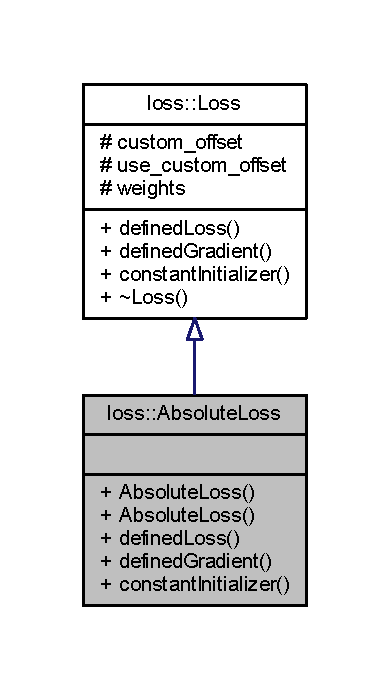
\includegraphics[width=187pt]{classloss_1_1_absolute_loss__inherit__graph}
\end{center}
\end{figure}


Collaboration diagram for loss\+:\+:Absolute\+Loss\+:
\nopagebreak
\begin{figure}[H]
\begin{center}
\leavevmode
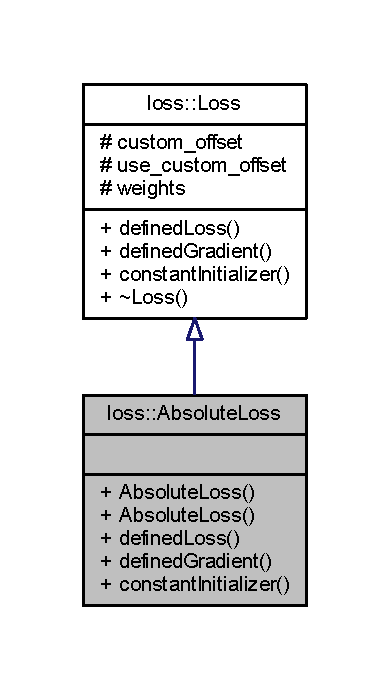
\includegraphics[width=187pt]{classloss_1_1_absolute_loss__coll__graph}
\end{center}
\end{figure}
\subsection*{Public Member Functions}
\begin{DoxyCompactItemize}
\item 
\mbox{\hyperlink{classloss_1_1_absolute_loss_a4b1416147d0573079f9d652097c1ab81}{Absolute\+Loss}} ()
\begin{DoxyCompactList}\small\item\em Default Constructor. \end{DoxyCompactList}\item 
\mbox{\hyperlink{classloss_1_1_absolute_loss_a3e056fbde0b63527bb9aadb0a4a8547a}{Absolute\+Loss}} (const double \&)
\begin{DoxyCompactList}\small\item\em Constructor to initialize custom offset. \end{DoxyCompactList}\item 
arma\+::vec \mbox{\hyperlink{classloss_1_1_absolute_loss_acfef6f0de3cfcccebd4bbfc04133cf1e}{defined\+Loss}} (const arma\+::vec \&, const arma\+::vec \&) const
\begin{DoxyCompactList}\small\item\em Specific loss function. \end{DoxyCompactList}\item 
arma\+::vec \mbox{\hyperlink{classloss_1_1_absolute_loss_a1886fc8ca065c6f0a207b7a8a0f8444d}{defined\+Gradient}} (const arma\+::vec \&, const arma\+::vec \&) const
\begin{DoxyCompactList}\small\item\em Gradient of loss functions for pseudo residuals. \end{DoxyCompactList}\item 
double \mbox{\hyperlink{classloss_1_1_absolute_loss_aa2ac5fb1fdf3ce0f48decd77d375ef76}{constant\+Initializer}} (const arma\+::vec \&) const
\begin{DoxyCompactList}\small\item\em Constant initialization of the empirical risk. \end{DoxyCompactList}\end{DoxyCompactItemize}
\subsection*{Additional Inherited Members}


\subsection{Detailed Description}
Absolute loss for regression tasks. 

{\bfseries \mbox{\hyperlink{classloss_1_1_loss}{Loss}} Function\+:} \[ L(y, f(x)) = \left| y - f(x) \right| \] {\bfseries Gradient\+:} \[ \frac{\delta}{\delta f(x)}\ L(y, f(x)) = \mathrm{sign}\left( f(x) - y \right) \] {\bfseries Initialization\+:} \[ \hat{f}^{[0]}(x) = \underset{c\in\mathbb{R}}{\mathrm{arg~min}}\ \frac{1}{n}\sum\limits_{i=1}^n L\left(y^{(i)}, c\right) = \mathrm{median}(y) \] 

\subsection{Constructor \& Destructor Documentation}
\mbox{\Hypertarget{classloss_1_1_absolute_loss_a4b1416147d0573079f9d652097c1ab81}\label{classloss_1_1_absolute_loss_a4b1416147d0573079f9d652097c1ab81}} 
\index{loss\+::\+Absolute\+Loss@{loss\+::\+Absolute\+Loss}!Absolute\+Loss@{Absolute\+Loss}}
\index{Absolute\+Loss@{Absolute\+Loss}!loss\+::\+Absolute\+Loss@{loss\+::\+Absolute\+Loss}}
\subsubsection{\texorpdfstring{Absolute\+Loss()}{AbsoluteLoss()}\hspace{0.1cm}{\footnotesize\ttfamily [1/2]}}
{\footnotesize\ttfamily loss\+::\+Absolute\+Loss\+::\+Absolute\+Loss (\begin{DoxyParamCaption}{ }\end{DoxyParamCaption})}



Default Constructor. 

Default constructor of {\ttfamily \mbox{\hyperlink{classloss_1_1_absolute_loss}{Absolute\+Loss}}} \mbox{\Hypertarget{classloss_1_1_absolute_loss_a3e056fbde0b63527bb9aadb0a4a8547a}\label{classloss_1_1_absolute_loss_a3e056fbde0b63527bb9aadb0a4a8547a}} 
\index{loss\+::\+Absolute\+Loss@{loss\+::\+Absolute\+Loss}!Absolute\+Loss@{Absolute\+Loss}}
\index{Absolute\+Loss@{Absolute\+Loss}!loss\+::\+Absolute\+Loss@{loss\+::\+Absolute\+Loss}}
\subsubsection{\texorpdfstring{Absolute\+Loss()}{AbsoluteLoss()}\hspace{0.1cm}{\footnotesize\ttfamily [2/2]}}
{\footnotesize\ttfamily loss\+::\+Absolute\+Loss\+::\+Absolute\+Loss (\begin{DoxyParamCaption}\item[{const double \&}]{custom\+\_\+offset0 }\end{DoxyParamCaption})}



Constructor to initialize custom offset. 

Constructor to initialize custom offset of {\ttfamily \mbox{\hyperlink{classloss_1_1_absolute_loss}{Absolute\+Loss}}}


\begin{DoxyParams}{Parameters}
{\em custom\+\_\+offset0} & {\ttfamily double} Offset which is used instead of the pre defined initialization \\
\hline
\end{DoxyParams}


\subsection{Member Function Documentation}
\mbox{\Hypertarget{classloss_1_1_absolute_loss_aa2ac5fb1fdf3ce0f48decd77d375ef76}\label{classloss_1_1_absolute_loss_aa2ac5fb1fdf3ce0f48decd77d375ef76}} 
\index{loss\+::\+Absolute\+Loss@{loss\+::\+Absolute\+Loss}!constant\+Initializer@{constant\+Initializer}}
\index{constant\+Initializer@{constant\+Initializer}!loss\+::\+Absolute\+Loss@{loss\+::\+Absolute\+Loss}}
\subsubsection{\texorpdfstring{constant\+Initializer()}{constantInitializer()}}
{\footnotesize\ttfamily double loss\+::\+Absolute\+Loss\+::constant\+Initializer (\begin{DoxyParamCaption}\item[{const arma\+::vec \&}]{true\+\_\+value }\end{DoxyParamCaption}) const\hspace{0.3cm}{\ttfamily [virtual]}}



Constant initialization of the empirical risk. 

Definition of the constant risk initialization (see description of the class)


\begin{DoxyParams}{Parameters}
{\em true\+\_\+value} & {\ttfamily arma\+::vec} True value of the response\\
\hline
\end{DoxyParams}
\begin{DoxyReturn}{Returns}
{\ttfamily double} constant which minimizes the empirical risk for the given true value 
\end{DoxyReturn}


Implements \mbox{\hyperlink{classloss_1_1_loss_a65fe7dcd9370e6a549b8d1cc95fc8798}{loss\+::\+Loss}}.

\mbox{\Hypertarget{classloss_1_1_absolute_loss_a1886fc8ca065c6f0a207b7a8a0f8444d}\label{classloss_1_1_absolute_loss_a1886fc8ca065c6f0a207b7a8a0f8444d}} 
\index{loss\+::\+Absolute\+Loss@{loss\+::\+Absolute\+Loss}!defined\+Gradient@{defined\+Gradient}}
\index{defined\+Gradient@{defined\+Gradient}!loss\+::\+Absolute\+Loss@{loss\+::\+Absolute\+Loss}}
\subsubsection{\texorpdfstring{defined\+Gradient()}{definedGradient()}}
{\footnotesize\ttfamily arma\+::vec loss\+::\+Absolute\+Loss\+::defined\+Gradient (\begin{DoxyParamCaption}\item[{const arma\+::vec \&}]{true\+\_\+value,  }\item[{const arma\+::vec \&}]{prediction }\end{DoxyParamCaption}) const\hspace{0.3cm}{\ttfamily [virtual]}}



Gradient of loss functions for pseudo residuals. 

Definition of the gradient of the loss function (see description of the class)


\begin{DoxyParams}{Parameters}
{\em true\+\_\+value} & {\ttfamily arma\+::vec} True value of the response \\
\hline
{\em prediction} & {\ttfamily arma\+::vec} Prediction of the true value\\
\hline
\end{DoxyParams}
\begin{DoxyReturn}{Returns}
{\ttfamily arma\+::vec} vector of elementwise application of the gradient 
\end{DoxyReturn}


Implements \mbox{\hyperlink{classloss_1_1_loss_a267a4de70747ade4b2d84ce35a448979}{loss\+::\+Loss}}.

\mbox{\Hypertarget{classloss_1_1_absolute_loss_acfef6f0de3cfcccebd4bbfc04133cf1e}\label{classloss_1_1_absolute_loss_acfef6f0de3cfcccebd4bbfc04133cf1e}} 
\index{loss\+::\+Absolute\+Loss@{loss\+::\+Absolute\+Loss}!defined\+Loss@{defined\+Loss}}
\index{defined\+Loss@{defined\+Loss}!loss\+::\+Absolute\+Loss@{loss\+::\+Absolute\+Loss}}
\subsubsection{\texorpdfstring{defined\+Loss()}{definedLoss()}}
{\footnotesize\ttfamily arma\+::vec loss\+::\+Absolute\+Loss\+::defined\+Loss (\begin{DoxyParamCaption}\item[{const arma\+::vec \&}]{true\+\_\+value,  }\item[{const arma\+::vec \&}]{prediction }\end{DoxyParamCaption}) const\hspace{0.3cm}{\ttfamily [virtual]}}



Specific loss function. 

Definition of the loss function (see description of the class)


\begin{DoxyParams}{Parameters}
{\em true\+\_\+value} & {\ttfamily arma\+::vec} True value of the response \\
\hline
{\em prediction} & {\ttfamily arma\+::vec} Prediction of the true value\\
\hline
\end{DoxyParams}
\begin{DoxyReturn}{Returns}
{\ttfamily arma\+::vec} vector of elementwise application of the loss function 
\end{DoxyReturn}


Implements \mbox{\hyperlink{classloss_1_1_loss_ae9f94dd9b8311397583ba3a9cb485e94}{loss\+::\+Loss}}.



The documentation for this class was generated from the following files\+:\begin{DoxyCompactItemize}
\item 
E\+:/\+One\+Drive/github\+\_\+repos/compboost/src/\mbox{\hyperlink{loss_8h}{loss.\+h}}\item 
E\+:/\+One\+Drive/github\+\_\+repos/compboost/src/\mbox{\hyperlink{loss_8cpp}{loss.\+cpp}}\end{DoxyCompactItemize}

\hypertarget{classblearner_1_1_baselearner}{}\section{blearner\+:\+:Baselearner Class Reference}
\label{classblearner_1_1_baselearner}\index{blearner\+::\+Baselearner@{blearner\+::\+Baselearner}}


{\ttfamily \#include $<$baselearner.\+h$>$}



Inheritance diagram for blearner\+:\+:Baselearner\+:\nopagebreak
\begin{figure}[H]
\begin{center}
\leavevmode
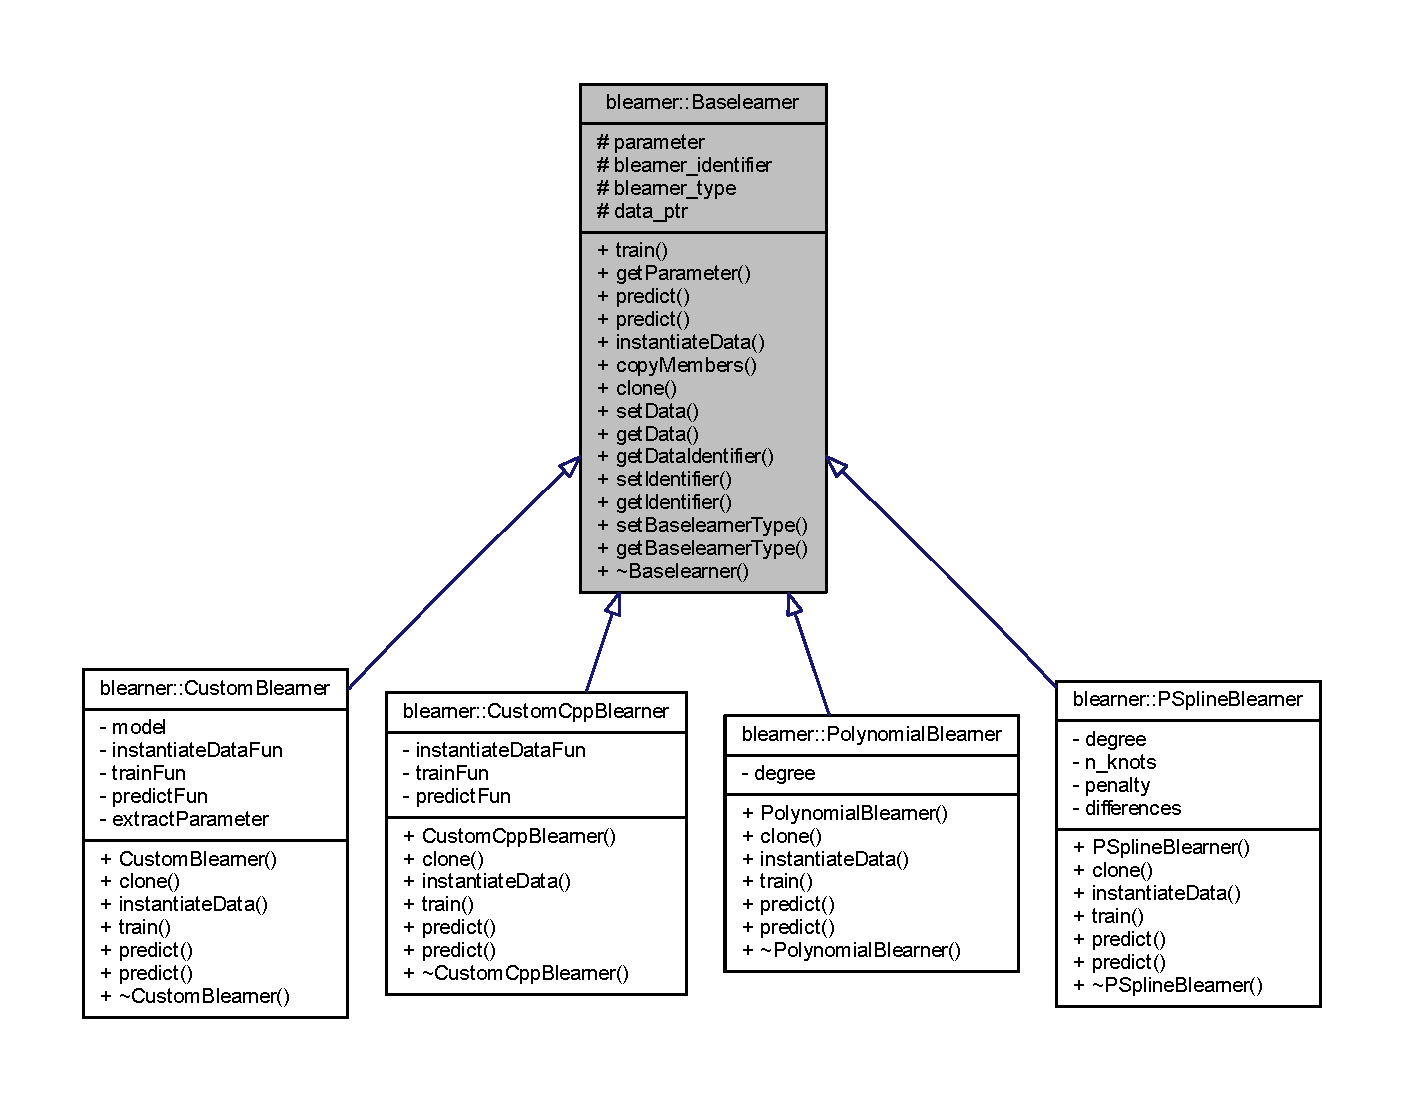
\includegraphics[width=350pt]{classblearner_1_1_baselearner__inherit__graph}
\end{center}
\end{figure}


Collaboration diagram for blearner\+:\+:Baselearner\+:\nopagebreak
\begin{figure}[H]
\begin{center}
\leavevmode
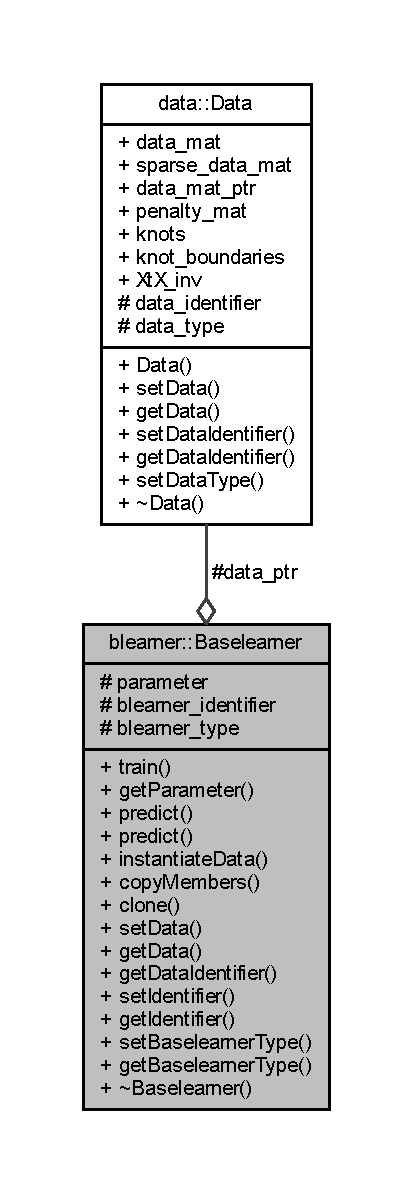
\includegraphics[width=198pt]{classblearner_1_1_baselearner__coll__graph}
\end{center}
\end{figure}
\subsection*{Public Member Functions}
\begin{DoxyCompactItemize}
\item 
virtual void \mbox{\hyperlink{classblearner_1_1_baselearner_a40e03ad070b9a03aae706d9ee8094b80}{train}} (const arma\+::vec \&)=0
\item 
arma\+::mat \mbox{\hyperlink{classblearner_1_1_baselearner_a3362fe72e1b653ec3664cae2397414ed}{get\+Parameter}} () const
\item 
virtual arma\+::mat \mbox{\hyperlink{classblearner_1_1_baselearner_ab37986047db43c84420fef2cef7fc20d}{predict}} ()=0
\item 
virtual arma\+::mat \mbox{\hyperlink{classblearner_1_1_baselearner_ae2ef5e018783578e02b3b5a33fa94eae}{predict}} (\mbox{\hyperlink{classdata_1_1_data}{data\+::\+Data}} $\ast$)=0
\item 
virtual arma\+::mat \mbox{\hyperlink{classblearner_1_1_baselearner_af01f1b8c4540927705ff79c3649489f7}{instantiate\+Data}} (const arma\+::mat \&)=0
\item 
void \mbox{\hyperlink{classblearner_1_1_baselearner_ae8f114ca7c497f03c80de5981c7f811d}{copy\+Members}} (const arma\+::mat \&, const std\+::string \&, \mbox{\hyperlink{classdata_1_1_data}{data\+::\+Data}} $\ast$)
\item 
virtual \mbox{\hyperlink{classblearner_1_1_baselearner}{Baselearner}} $\ast$ \mbox{\hyperlink{classblearner_1_1_baselearner_a8e12c6739f085917a7d2da6570c51a21}{clone}} ()=0
\item 
void \mbox{\hyperlink{classblearner_1_1_baselearner_a29122c6125ef6ec03ad84602b3e2d0d4}{set\+Data}} (\mbox{\hyperlink{classdata_1_1_data}{data\+::\+Data}} $\ast$)
\item 
arma\+::mat \mbox{\hyperlink{classblearner_1_1_baselearner_af3a360bb039447610e9928956384c05d}{get\+Data}} () const
\item 
std\+::string \mbox{\hyperlink{classblearner_1_1_baselearner_a2393dc1e3cf90919ebbbd237fe303860}{get\+Data\+Identifier}} () const
\item 
void \mbox{\hyperlink{classblearner_1_1_baselearner_a6669906a481cbdd516dce8df6f6e5b76}{set\+Identifier}} (const std\+::string \&)
\item 
std\+::string \mbox{\hyperlink{classblearner_1_1_baselearner_aa10fa4301aeb37f6e8c18457541c3be7}{get\+Identifier}} () const
\item 
void \mbox{\hyperlink{classblearner_1_1_baselearner_a8d78e851bae5f5b93dc46eb13d2d1ee1}{set\+Baselearner\+Type}} (const std\+::string \&)
\item 
std\+::string \mbox{\hyperlink{classblearner_1_1_baselearner_acec1a791f94eed39d2662c245e7f6b51}{get\+Baselearner\+Type}} () const
\item 
virtual \mbox{\hyperlink{classblearner_1_1_baselearner_a1ada1c47d71e60bec80ab033ffa40813}{$\sim$\+Baselearner}} ()
\end{DoxyCompactItemize}
\subsection*{Protected Attributes}
\begin{DoxyCompactItemize}
\item 
arma\+::mat \mbox{\hyperlink{classblearner_1_1_baselearner_a56e401f574b274d65e364493277f3247}{parameter}}
\item 
std\+::string \mbox{\hyperlink{classblearner_1_1_baselearner_a7112e057b2b29bb6529df6df3b8a9165}{blearner\+\_\+identifier}}
\item 
std\+::string \mbox{\hyperlink{classblearner_1_1_baselearner_aed6406144af33850b3cb9222dddf3f57}{blearner\+\_\+type}}
\item 
\mbox{\hyperlink{classdata_1_1_data}{data\+::\+Data}} $\ast$ \mbox{\hyperlink{classblearner_1_1_baselearner_a5b5cfab411ff94a13bcce4ca0dd4e507}{data\+\_\+ptr}}
\end{DoxyCompactItemize}


\subsection{Constructor \& Destructor Documentation}
\mbox{\Hypertarget{classblearner_1_1_baselearner_a1ada1c47d71e60bec80ab033ffa40813}\label{classblearner_1_1_baselearner_a1ada1c47d71e60bec80ab033ffa40813}} 
\index{blearner\+::\+Baselearner@{blearner\+::\+Baselearner}!````~Baselearner@{$\sim$\+Baselearner}}
\index{````~Baselearner@{$\sim$\+Baselearner}!blearner\+::\+Baselearner@{blearner\+::\+Baselearner}}
\subsubsection{\texorpdfstring{$\sim$\+Baselearner()}{~Baselearner()}}
{\footnotesize\ttfamily blearner\+::\+Baselearner\+::$\sim$\+Baselearner (\begin{DoxyParamCaption}{ }\end{DoxyParamCaption})\hspace{0.3cm}{\ttfamily [virtual]}}



\subsection{Member Function Documentation}
\mbox{\Hypertarget{classblearner_1_1_baselearner_a8e12c6739f085917a7d2da6570c51a21}\label{classblearner_1_1_baselearner_a8e12c6739f085917a7d2da6570c51a21}} 
\index{blearner\+::\+Baselearner@{blearner\+::\+Baselearner}!clone@{clone}}
\index{clone@{clone}!blearner\+::\+Baselearner@{blearner\+::\+Baselearner}}
\subsubsection{\texorpdfstring{clone()}{clone()}}
{\footnotesize\ttfamily virtual \mbox{\hyperlink{classblearner_1_1_baselearner}{Baselearner}}$\ast$ blearner\+::\+Baselearner\+::clone (\begin{DoxyParamCaption}{ }\end{DoxyParamCaption})\hspace{0.3cm}{\ttfamily [pure virtual]}}



Implemented in \mbox{\hyperlink{classblearner_1_1_custom_cpp_blearner_a8b76705131d397974cd208fdcfd70496}{blearner\+::\+Custom\+Cpp\+Blearner}}, \mbox{\hyperlink{classblearner_1_1_custom_blearner_a7ceeee2b7fffd11f376018bc1d3cfba1}{blearner\+::\+Custom\+Blearner}}, and \mbox{\hyperlink{classblearner_1_1_polynomial_blearner_a4a93ace818c330e5d1f572108ba061c0}{blearner\+::\+Polynomial\+Blearner}}.

Here is the caller graph for this function\+:\nopagebreak
\begin{figure}[H]
\begin{center}
\leavevmode
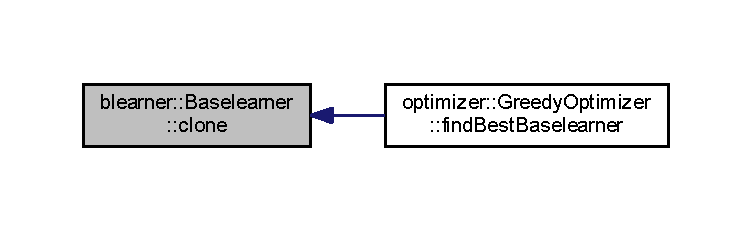
\includegraphics[width=350pt]{classblearner_1_1_baselearner_a8e12c6739f085917a7d2da6570c51a21_icgraph}
\end{center}
\end{figure}
\mbox{\Hypertarget{classblearner_1_1_baselearner_ae8f114ca7c497f03c80de5981c7f811d}\label{classblearner_1_1_baselearner_ae8f114ca7c497f03c80de5981c7f811d}} 
\index{blearner\+::\+Baselearner@{blearner\+::\+Baselearner}!copy\+Members@{copy\+Members}}
\index{copy\+Members@{copy\+Members}!blearner\+::\+Baselearner@{blearner\+::\+Baselearner}}
\subsubsection{\texorpdfstring{copy\+Members()}{copyMembers()}}
{\footnotesize\ttfamily void blearner\+::\+Baselearner\+::copy\+Members (\begin{DoxyParamCaption}\item[{const arma\+::mat \&}]{parameter0,  }\item[{const std\+::string \&}]{blearner\+\_\+identifier0,  }\item[{\mbox{\hyperlink{classdata_1_1_data}{data\+::\+Data}} $\ast$}]{data0 }\end{DoxyParamCaption})}

Here is the caller graph for this function\+:\nopagebreak
\begin{figure}[H]
\begin{center}
\leavevmode
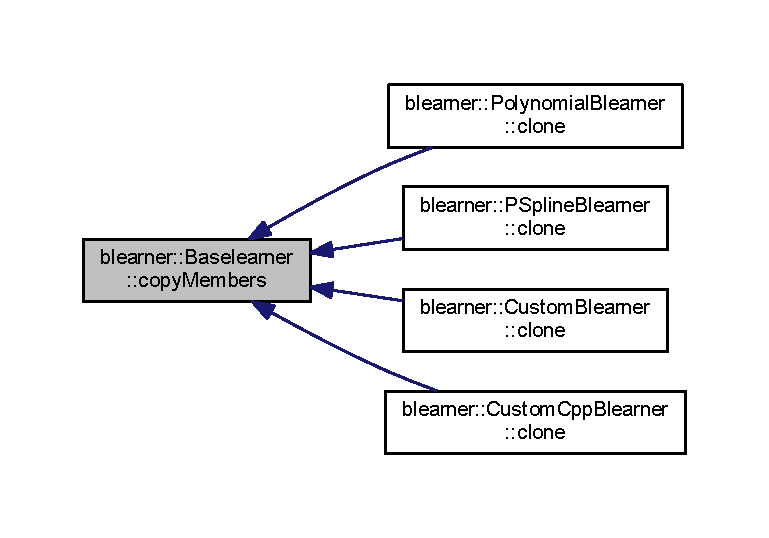
\includegraphics[width=350pt]{classblearner_1_1_baselearner_ae8f114ca7c497f03c80de5981c7f811d_icgraph}
\end{center}
\end{figure}
\mbox{\Hypertarget{classblearner_1_1_baselearner_acec1a791f94eed39d2662c245e7f6b51}\label{classblearner_1_1_baselearner_acec1a791f94eed39d2662c245e7f6b51}} 
\index{blearner\+::\+Baselearner@{blearner\+::\+Baselearner}!get\+Baselearner\+Type@{get\+Baselearner\+Type}}
\index{get\+Baselearner\+Type@{get\+Baselearner\+Type}!blearner\+::\+Baselearner@{blearner\+::\+Baselearner}}
\subsubsection{\texorpdfstring{get\+Baselearner\+Type()}{getBaselearnerType()}}
{\footnotesize\ttfamily std\+::string blearner\+::\+Baselearner\+::get\+Baselearner\+Type (\begin{DoxyParamCaption}{ }\end{DoxyParamCaption}) const}

Here is the caller graph for this function\+:\nopagebreak
\begin{figure}[H]
\begin{center}
\leavevmode
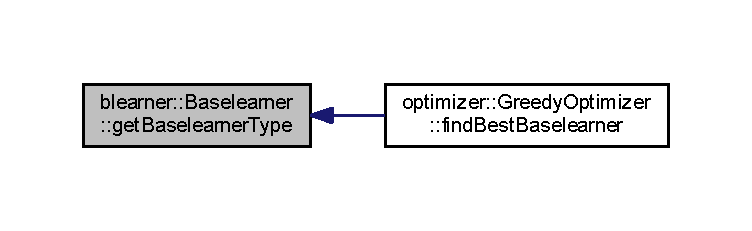
\includegraphics[width=350pt]{classblearner_1_1_baselearner_acec1a791f94eed39d2662c245e7f6b51_icgraph}
\end{center}
\end{figure}
\mbox{\Hypertarget{classblearner_1_1_baselearner_af3a360bb039447610e9928956384c05d}\label{classblearner_1_1_baselearner_af3a360bb039447610e9928956384c05d}} 
\index{blearner\+::\+Baselearner@{blearner\+::\+Baselearner}!get\+Data@{get\+Data}}
\index{get\+Data@{get\+Data}!blearner\+::\+Baselearner@{blearner\+::\+Baselearner}}
\subsubsection{\texorpdfstring{get\+Data()}{getData()}}
{\footnotesize\ttfamily arma\+::mat blearner\+::\+Baselearner\+::get\+Data (\begin{DoxyParamCaption}{ }\end{DoxyParamCaption}) const}

Here is the call graph for this function\+:\nopagebreak
\begin{figure}[H]
\begin{center}
\leavevmode
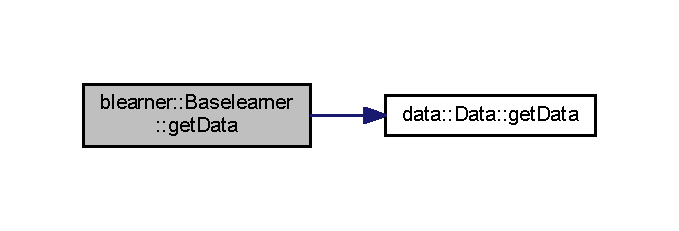
\includegraphics[width=326pt]{classblearner_1_1_baselearner_af3a360bb039447610e9928956384c05d_cgraph}
\end{center}
\end{figure}
\mbox{\Hypertarget{classblearner_1_1_baselearner_a2393dc1e3cf90919ebbbd237fe303860}\label{classblearner_1_1_baselearner_a2393dc1e3cf90919ebbbd237fe303860}} 
\index{blearner\+::\+Baselearner@{blearner\+::\+Baselearner}!get\+Data\+Identifier@{get\+Data\+Identifier}}
\index{get\+Data\+Identifier@{get\+Data\+Identifier}!blearner\+::\+Baselearner@{blearner\+::\+Baselearner}}
\subsubsection{\texorpdfstring{get\+Data\+Identifier()}{getDataIdentifier()}}
{\footnotesize\ttfamily std\+::string blearner\+::\+Baselearner\+::get\+Data\+Identifier (\begin{DoxyParamCaption}{ }\end{DoxyParamCaption}) const}

Here is the call graph for this function\+:\nopagebreak
\begin{figure}[H]
\begin{center}
\leavevmode
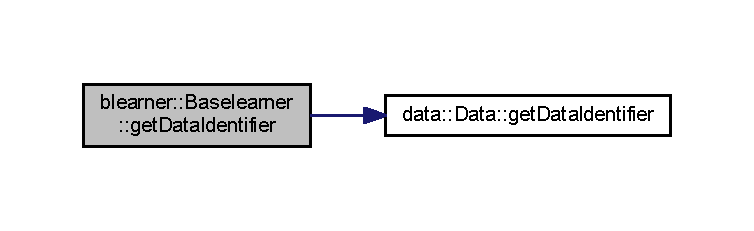
\includegraphics[width=350pt]{classblearner_1_1_baselearner_a2393dc1e3cf90919ebbbd237fe303860_cgraph}
\end{center}
\end{figure}
Here is the caller graph for this function\+:\nopagebreak
\begin{figure}[H]
\begin{center}
\leavevmode
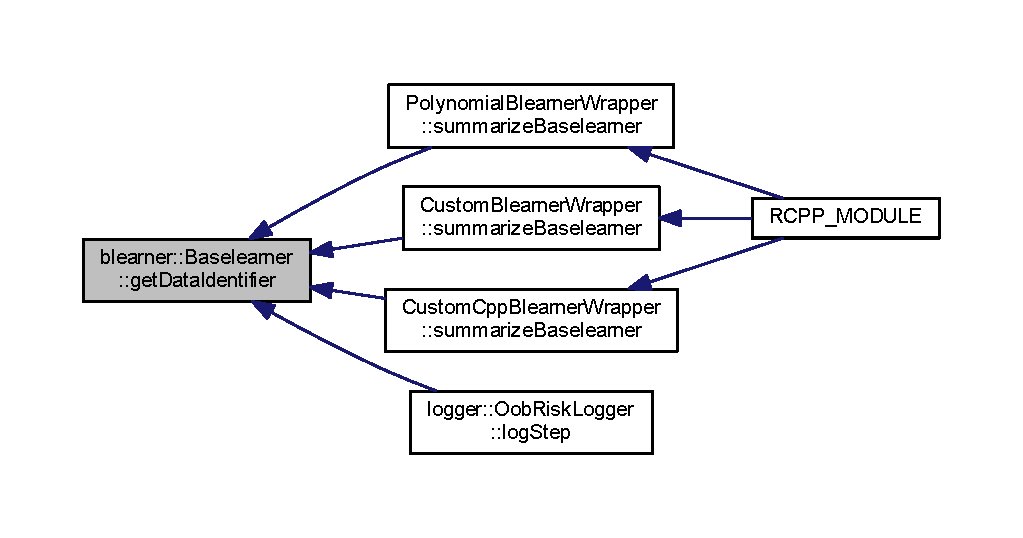
\includegraphics[width=350pt]{classblearner_1_1_baselearner_a2393dc1e3cf90919ebbbd237fe303860_icgraph}
\end{center}
\end{figure}
\mbox{\Hypertarget{classblearner_1_1_baselearner_aa10fa4301aeb37f6e8c18457541c3be7}\label{classblearner_1_1_baselearner_aa10fa4301aeb37f6e8c18457541c3be7}} 
\index{blearner\+::\+Baselearner@{blearner\+::\+Baselearner}!get\+Identifier@{get\+Identifier}}
\index{get\+Identifier@{get\+Identifier}!blearner\+::\+Baselearner@{blearner\+::\+Baselearner}}
\subsubsection{\texorpdfstring{get\+Identifier()}{getIdentifier()}}
{\footnotesize\ttfamily std\+::string blearner\+::\+Baselearner\+::get\+Identifier (\begin{DoxyParamCaption}{ }\end{DoxyParamCaption}) const}

Here is the caller graph for this function\+:\nopagebreak
\begin{figure}[H]
\begin{center}
\leavevmode
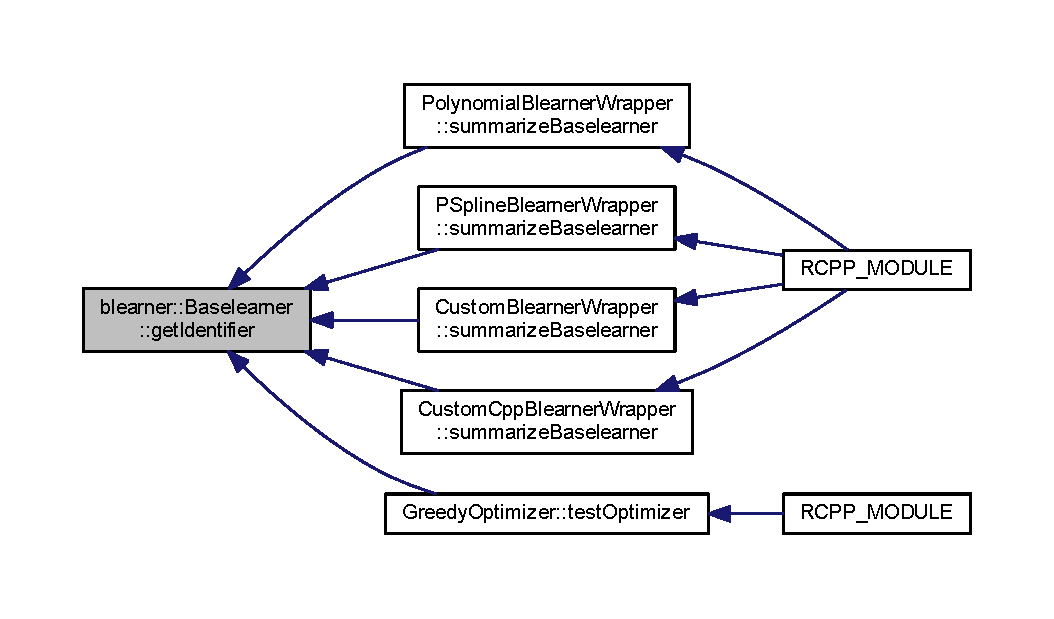
\includegraphics[width=350pt]{classblearner_1_1_baselearner_aa10fa4301aeb37f6e8c18457541c3be7_icgraph}
\end{center}
\end{figure}
\mbox{\Hypertarget{classblearner_1_1_baselearner_a3362fe72e1b653ec3664cae2397414ed}\label{classblearner_1_1_baselearner_a3362fe72e1b653ec3664cae2397414ed}} 
\index{blearner\+::\+Baselearner@{blearner\+::\+Baselearner}!get\+Parameter@{get\+Parameter}}
\index{get\+Parameter@{get\+Parameter}!blearner\+::\+Baselearner@{blearner\+::\+Baselearner}}
\subsubsection{\texorpdfstring{get\+Parameter()}{getParameter()}}
{\footnotesize\ttfamily arma\+::mat blearner\+::\+Baselearner\+::get\+Parameter (\begin{DoxyParamCaption}{ }\end{DoxyParamCaption}) const}

Here is the caller graph for this function\+:\nopagebreak
\begin{figure}[H]
\begin{center}
\leavevmode
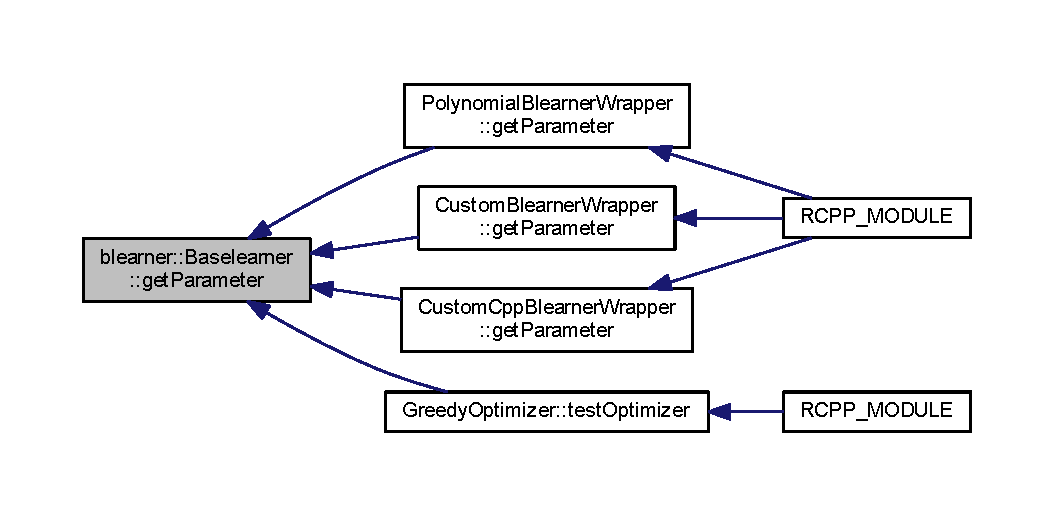
\includegraphics[width=350pt]{classblearner_1_1_baselearner_a3362fe72e1b653ec3664cae2397414ed_icgraph}
\end{center}
\end{figure}
\mbox{\Hypertarget{classblearner_1_1_baselearner_af01f1b8c4540927705ff79c3649489f7}\label{classblearner_1_1_baselearner_af01f1b8c4540927705ff79c3649489f7}} 
\index{blearner\+::\+Baselearner@{blearner\+::\+Baselearner}!instantiate\+Data@{instantiate\+Data}}
\index{instantiate\+Data@{instantiate\+Data}!blearner\+::\+Baselearner@{blearner\+::\+Baselearner}}
\subsubsection{\texorpdfstring{instantiate\+Data()}{instantiateData()}}
{\footnotesize\ttfamily virtual arma\+::mat blearner\+::\+Baselearner\+::instantiate\+Data (\begin{DoxyParamCaption}\item[{const arma\+::mat \&}]{ }\end{DoxyParamCaption})\hspace{0.3cm}{\ttfamily [pure virtual]}}



Implemented in \mbox{\hyperlink{classblearner_1_1_custom_cpp_blearner_a14607a1d1f312d46a3024b37085c146d}{blearner\+::\+Custom\+Cpp\+Blearner}}, \mbox{\hyperlink{classblearner_1_1_custom_blearner_a18971368219f6948456b8e60c20b6968}{blearner\+::\+Custom\+Blearner}}, and \mbox{\hyperlink{classblearner_1_1_polynomial_blearner_a5d3a44e8a4a8155ac24ee05e2c68af75}{blearner\+::\+Polynomial\+Blearner}}.

Here is the caller graph for this function\+:\nopagebreak
\begin{figure}[H]
\begin{center}
\leavevmode
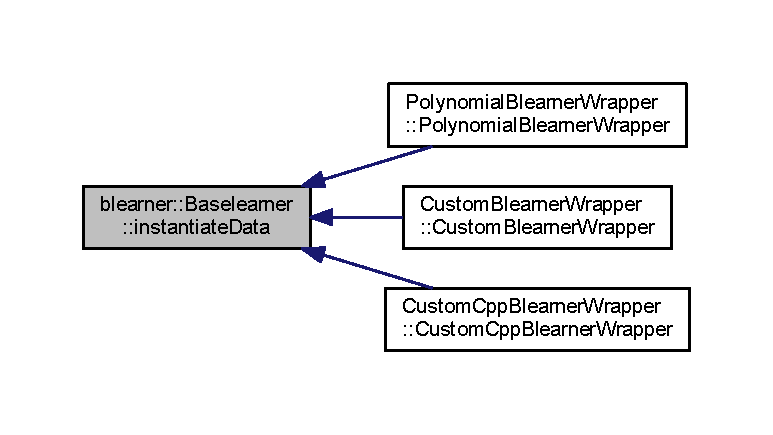
\includegraphics[width=350pt]{classblearner_1_1_baselearner_af01f1b8c4540927705ff79c3649489f7_icgraph}
\end{center}
\end{figure}
\mbox{\Hypertarget{classblearner_1_1_baselearner_ab37986047db43c84420fef2cef7fc20d}\label{classblearner_1_1_baselearner_ab37986047db43c84420fef2cef7fc20d}} 
\index{blearner\+::\+Baselearner@{blearner\+::\+Baselearner}!predict@{predict}}
\index{predict@{predict}!blearner\+::\+Baselearner@{blearner\+::\+Baselearner}}
\subsubsection{\texorpdfstring{predict()}{predict()}\hspace{0.1cm}{\footnotesize\ttfamily [1/2]}}
{\footnotesize\ttfamily virtual arma\+::mat blearner\+::\+Baselearner\+::predict (\begin{DoxyParamCaption}{ }\end{DoxyParamCaption})\hspace{0.3cm}{\ttfamily [pure virtual]}}



Implemented in \mbox{\hyperlink{classblearner_1_1_custom_cpp_blearner_aa17db5f5627b8251b2d8484d92e783b9}{blearner\+::\+Custom\+Cpp\+Blearner}}, \mbox{\hyperlink{classblearner_1_1_custom_blearner_a20b5fe06512aa73478b9f934e1c81c31}{blearner\+::\+Custom\+Blearner}}, and \mbox{\hyperlink{classblearner_1_1_polynomial_blearner_a422569884414d31db5a2b770b22176c3}{blearner\+::\+Polynomial\+Blearner}}.

Here is the caller graph for this function\+:\nopagebreak
\begin{figure}[H]
\begin{center}
\leavevmode
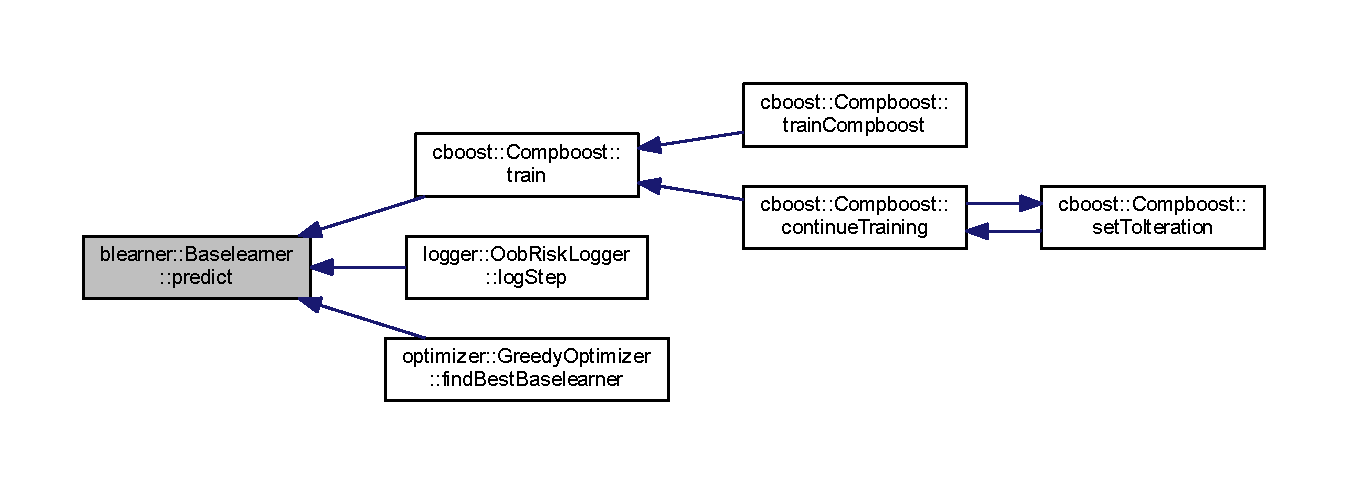
\includegraphics[width=350pt]{classblearner_1_1_baselearner_ab37986047db43c84420fef2cef7fc20d_icgraph}
\end{center}
\end{figure}
\mbox{\Hypertarget{classblearner_1_1_baselearner_ae2ef5e018783578e02b3b5a33fa94eae}\label{classblearner_1_1_baselearner_ae2ef5e018783578e02b3b5a33fa94eae}} 
\index{blearner\+::\+Baselearner@{blearner\+::\+Baselearner}!predict@{predict}}
\index{predict@{predict}!blearner\+::\+Baselearner@{blearner\+::\+Baselearner}}
\subsubsection{\texorpdfstring{predict()}{predict()}\hspace{0.1cm}{\footnotesize\ttfamily [2/2]}}
{\footnotesize\ttfamily virtual arma\+::mat blearner\+::\+Baselearner\+::predict (\begin{DoxyParamCaption}\item[{\mbox{\hyperlink{classdata_1_1_data}{data\+::\+Data}} $\ast$}]{ }\end{DoxyParamCaption})\hspace{0.3cm}{\ttfamily [pure virtual]}}



Implemented in \mbox{\hyperlink{classblearner_1_1_custom_cpp_blearner_af2326171640e94c3a00f813781710208}{blearner\+::\+Custom\+Cpp\+Blearner}}, \mbox{\hyperlink{classblearner_1_1_custom_blearner_a401a479834eb3896260cb57b4551ceb4}{blearner\+::\+Custom\+Blearner}}, and \mbox{\hyperlink{classblearner_1_1_polynomial_blearner_ae321c17adaab23b0d27685920c2608af}{blearner\+::\+Polynomial\+Blearner}}.

\mbox{\Hypertarget{classblearner_1_1_baselearner_a8d78e851bae5f5b93dc46eb13d2d1ee1}\label{classblearner_1_1_baselearner_a8d78e851bae5f5b93dc46eb13d2d1ee1}} 
\index{blearner\+::\+Baselearner@{blearner\+::\+Baselearner}!set\+Baselearner\+Type@{set\+Baselearner\+Type}}
\index{set\+Baselearner\+Type@{set\+Baselearner\+Type}!blearner\+::\+Baselearner@{blearner\+::\+Baselearner}}
\subsubsection{\texorpdfstring{set\+Baselearner\+Type()}{setBaselearnerType()}}
{\footnotesize\ttfamily void blearner\+::\+Baselearner\+::set\+Baselearner\+Type (\begin{DoxyParamCaption}\item[{const std\+::string \&}]{blearner\+\_\+type0 }\end{DoxyParamCaption})}

Here is the caller graph for this function\+:\nopagebreak
\begin{figure}[H]
\begin{center}
\leavevmode
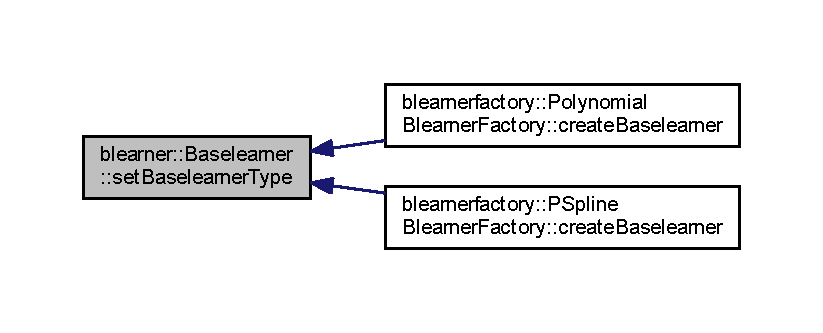
\includegraphics[width=350pt]{classblearner_1_1_baselearner_a8d78e851bae5f5b93dc46eb13d2d1ee1_icgraph}
\end{center}
\end{figure}
\mbox{\Hypertarget{classblearner_1_1_baselearner_a29122c6125ef6ec03ad84602b3e2d0d4}\label{classblearner_1_1_baselearner_a29122c6125ef6ec03ad84602b3e2d0d4}} 
\index{blearner\+::\+Baselearner@{blearner\+::\+Baselearner}!set\+Data@{set\+Data}}
\index{set\+Data@{set\+Data}!blearner\+::\+Baselearner@{blearner\+::\+Baselearner}}
\subsubsection{\texorpdfstring{set\+Data()}{setData()}}
{\footnotesize\ttfamily void blearner\+::\+Baselearner\+::set\+Data (\begin{DoxyParamCaption}\item[{\mbox{\hyperlink{classdata_1_1_data}{data\+::\+Data}} $\ast$}]{data }\end{DoxyParamCaption})}

Here is the caller graph for this function\+:\nopagebreak
\begin{figure}[H]
\begin{center}
\leavevmode
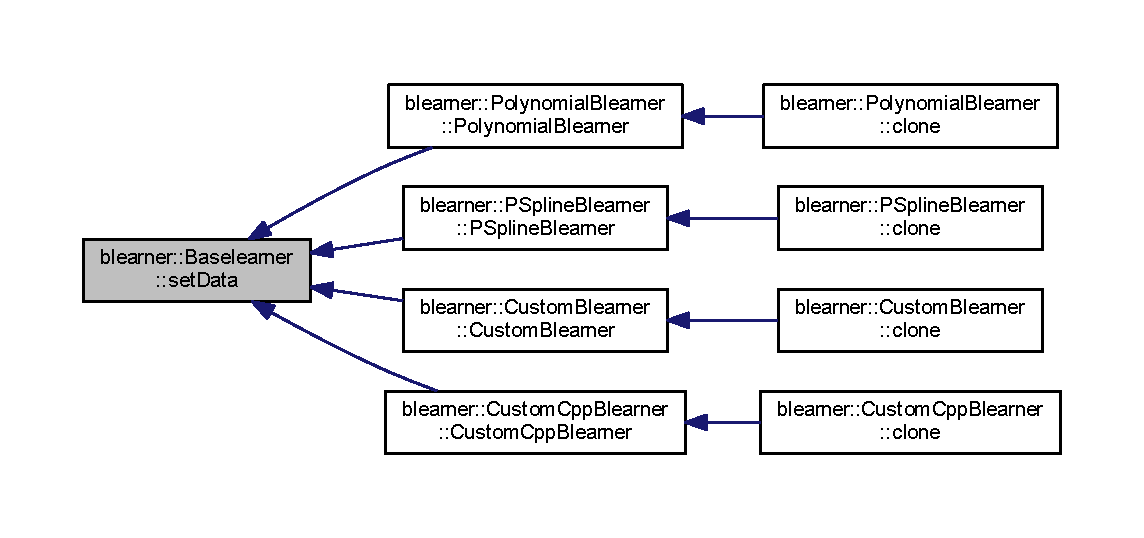
\includegraphics[width=350pt]{classblearner_1_1_baselearner_a29122c6125ef6ec03ad84602b3e2d0d4_icgraph}
\end{center}
\end{figure}
\mbox{\Hypertarget{classblearner_1_1_baselearner_a6669906a481cbdd516dce8df6f6e5b76}\label{classblearner_1_1_baselearner_a6669906a481cbdd516dce8df6f6e5b76}} 
\index{blearner\+::\+Baselearner@{blearner\+::\+Baselearner}!set\+Identifier@{set\+Identifier}}
\index{set\+Identifier@{set\+Identifier}!blearner\+::\+Baselearner@{blearner\+::\+Baselearner}}
\subsubsection{\texorpdfstring{set\+Identifier()}{setIdentifier()}}
{\footnotesize\ttfamily void blearner\+::\+Baselearner\+::set\+Identifier (\begin{DoxyParamCaption}\item[{const std\+::string \&}]{id0 }\end{DoxyParamCaption})}

Here is the caller graph for this function\+:\nopagebreak
\begin{figure}[H]
\begin{center}
\leavevmode
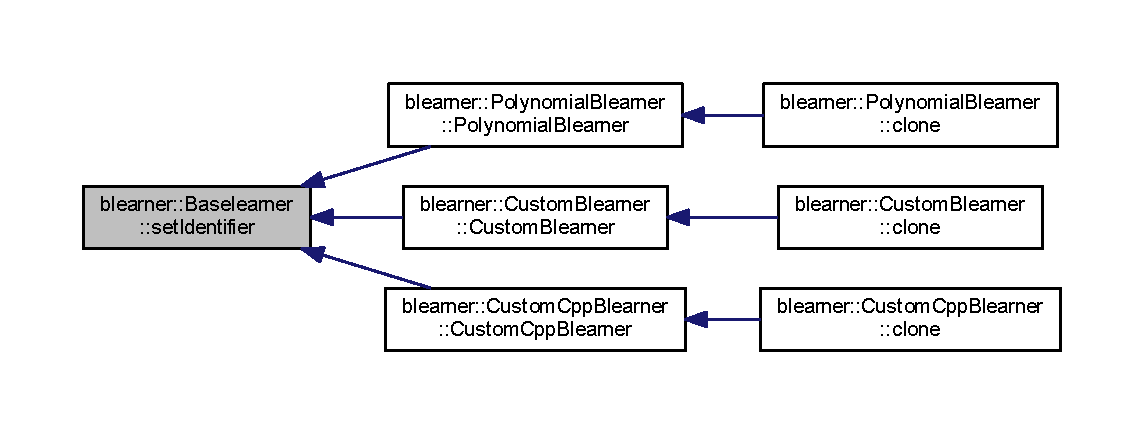
\includegraphics[width=350pt]{classblearner_1_1_baselearner_a6669906a481cbdd516dce8df6f6e5b76_icgraph}
\end{center}
\end{figure}
\mbox{\Hypertarget{classblearner_1_1_baselearner_a40e03ad070b9a03aae706d9ee8094b80}\label{classblearner_1_1_baselearner_a40e03ad070b9a03aae706d9ee8094b80}} 
\index{blearner\+::\+Baselearner@{blearner\+::\+Baselearner}!train@{train}}
\index{train@{train}!blearner\+::\+Baselearner@{blearner\+::\+Baselearner}}
\subsubsection{\texorpdfstring{train()}{train()}}
{\footnotesize\ttfamily virtual void blearner\+::\+Baselearner\+::train (\begin{DoxyParamCaption}\item[{const arma\+::vec \&}]{ }\end{DoxyParamCaption})\hspace{0.3cm}{\ttfamily [pure virtual]}}



Implemented in \mbox{\hyperlink{classblearner_1_1_custom_cpp_blearner_aa71b777d7092a3d9b47a9bed125eb0f9}{blearner\+::\+Custom\+Cpp\+Blearner}}, \mbox{\hyperlink{classblearner_1_1_custom_blearner_a4726c5b861b67817f7b3eb61d8f6c0d7}{blearner\+::\+Custom\+Blearner}}, and \mbox{\hyperlink{classblearner_1_1_polynomial_blearner_acf24025a73293a2569450dd4659e0997}{blearner\+::\+Polynomial\+Blearner}}.

Here is the caller graph for this function\+:\nopagebreak
\begin{figure}[H]
\begin{center}
\leavevmode
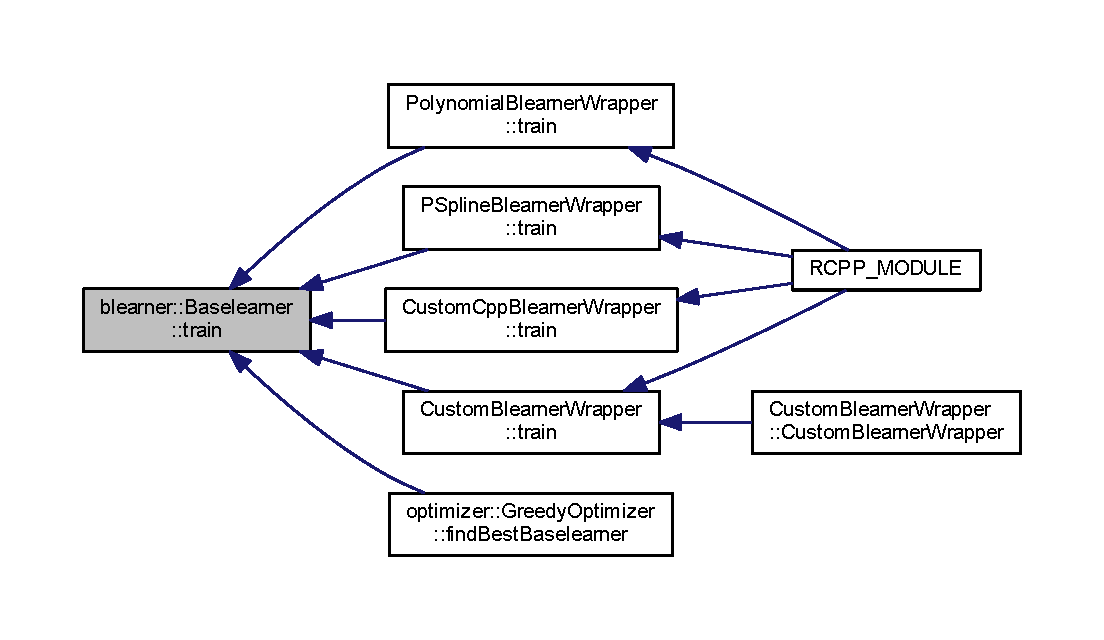
\includegraphics[width=350pt]{classblearner_1_1_baselearner_a40e03ad070b9a03aae706d9ee8094b80_icgraph}
\end{center}
\end{figure}


\subsection{Member Data Documentation}
\mbox{\Hypertarget{classblearner_1_1_baselearner_a7112e057b2b29bb6529df6df3b8a9165}\label{classblearner_1_1_baselearner_a7112e057b2b29bb6529df6df3b8a9165}} 
\index{blearner\+::\+Baselearner@{blearner\+::\+Baselearner}!blearner\+\_\+identifier@{blearner\+\_\+identifier}}
\index{blearner\+\_\+identifier@{blearner\+\_\+identifier}!blearner\+::\+Baselearner@{blearner\+::\+Baselearner}}
\subsubsection{\texorpdfstring{blearner\+\_\+identifier}{blearner\_identifier}}
{\footnotesize\ttfamily std\+::string blearner\+::\+Baselearner\+::blearner\+\_\+identifier\hspace{0.3cm}{\ttfamily [protected]}}

\mbox{\Hypertarget{classblearner_1_1_baselearner_aed6406144af33850b3cb9222dddf3f57}\label{classblearner_1_1_baselearner_aed6406144af33850b3cb9222dddf3f57}} 
\index{blearner\+::\+Baselearner@{blearner\+::\+Baselearner}!blearner\+\_\+type@{blearner\+\_\+type}}
\index{blearner\+\_\+type@{blearner\+\_\+type}!blearner\+::\+Baselearner@{blearner\+::\+Baselearner}}
\subsubsection{\texorpdfstring{blearner\+\_\+type}{blearner\_type}}
{\footnotesize\ttfamily std\+::string blearner\+::\+Baselearner\+::blearner\+\_\+type\hspace{0.3cm}{\ttfamily [protected]}}

\mbox{\Hypertarget{classblearner_1_1_baselearner_a5b5cfab411ff94a13bcce4ca0dd4e507}\label{classblearner_1_1_baselearner_a5b5cfab411ff94a13bcce4ca0dd4e507}} 
\index{blearner\+::\+Baselearner@{blearner\+::\+Baselearner}!data\+\_\+ptr@{data\+\_\+ptr}}
\index{data\+\_\+ptr@{data\+\_\+ptr}!blearner\+::\+Baselearner@{blearner\+::\+Baselearner}}
\subsubsection{\texorpdfstring{data\+\_\+ptr}{data\_ptr}}
{\footnotesize\ttfamily \mbox{\hyperlink{classdata_1_1_data}{data\+::\+Data}}$\ast$ blearner\+::\+Baselearner\+::data\+\_\+ptr\hspace{0.3cm}{\ttfamily [protected]}}

\mbox{\Hypertarget{classblearner_1_1_baselearner_a56e401f574b274d65e364493277f3247}\label{classblearner_1_1_baselearner_a56e401f574b274d65e364493277f3247}} 
\index{blearner\+::\+Baselearner@{blearner\+::\+Baselearner}!parameter@{parameter}}
\index{parameter@{parameter}!blearner\+::\+Baselearner@{blearner\+::\+Baselearner}}
\subsubsection{\texorpdfstring{parameter}{parameter}}
{\footnotesize\ttfamily arma\+::mat blearner\+::\+Baselearner\+::parameter\hspace{0.3cm}{\ttfamily [protected]}}



The documentation for this class was generated from the following files\+:\begin{DoxyCompactItemize}
\item 
E\+:/\+One\+Drive/github\+\_\+repos/compboost/src/\mbox{\hyperlink{baselearner_8h}{baselearner.\+h}}\item 
E\+:/\+One\+Drive/github\+\_\+repos/compboost/src/\mbox{\hyperlink{baselearner_8cpp}{baselearner.\+cpp}}\end{DoxyCompactItemize}

\hypertarget{classblearnerfactory_1_1_baselearner_factory}{}\section{blearnerfactory\+:\+:Baselearner\+Factory Class Reference}
\label{classblearnerfactory_1_1_baselearner_factory}\index{blearnerfactory\+::\+Baselearner\+Factory@{blearnerfactory\+::\+Baselearner\+Factory}}


{\ttfamily \#include $<$baselearner\+\_\+factory.\+h$>$}



Inheritance diagram for blearnerfactory\+:\+:Baselearner\+Factory\+:\nopagebreak
\begin{figure}[H]
\begin{center}
\leavevmode
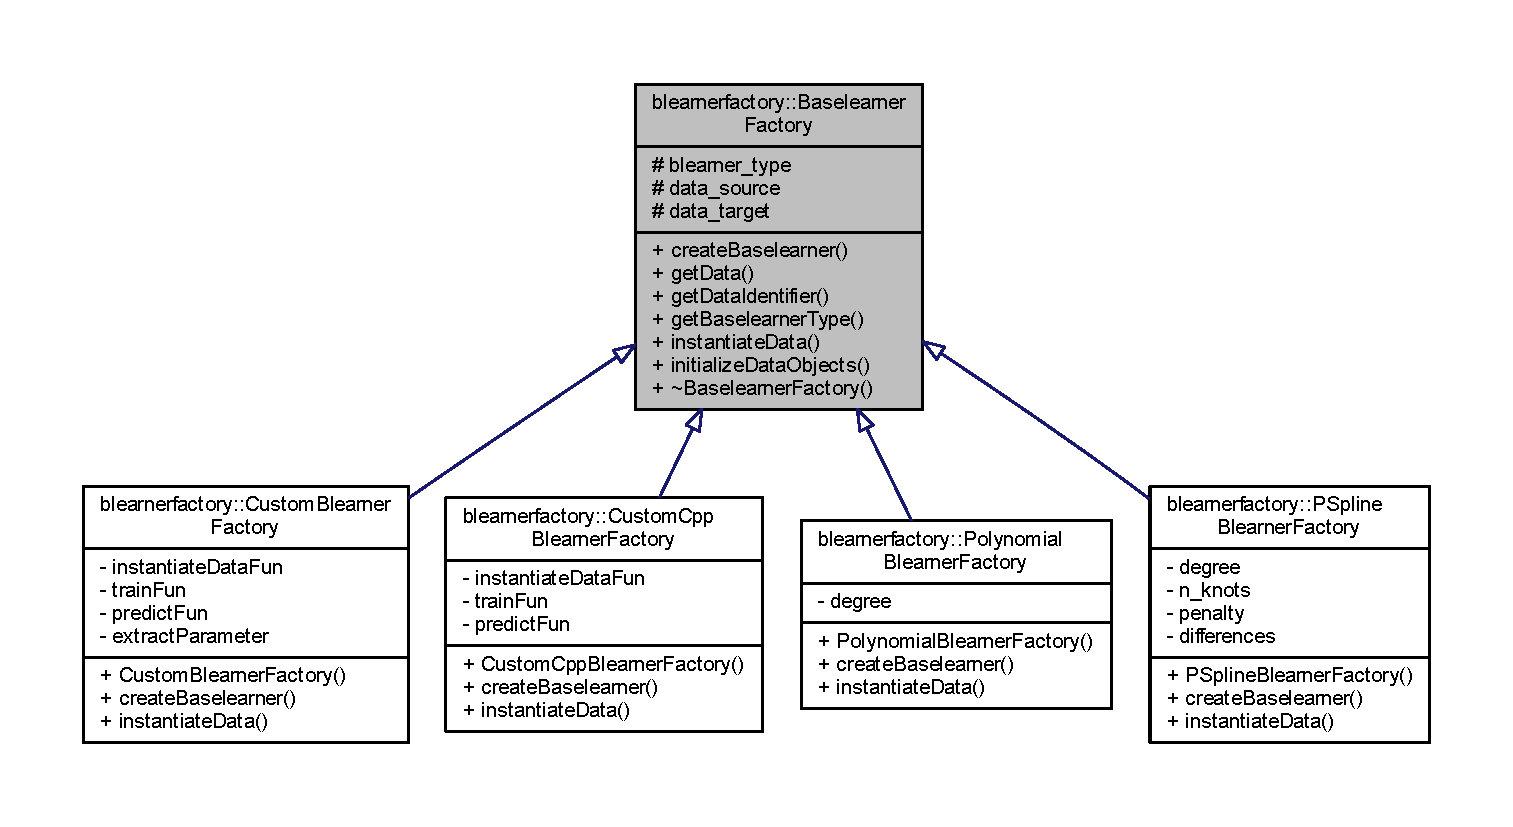
\includegraphics[width=350pt]{classblearnerfactory_1_1_baselearner_factory__inherit__graph}
\end{center}
\end{figure}


Collaboration diagram for blearnerfactory\+:\+:Baselearner\+Factory\+:\nopagebreak
\begin{figure}[H]
\begin{center}
\leavevmode
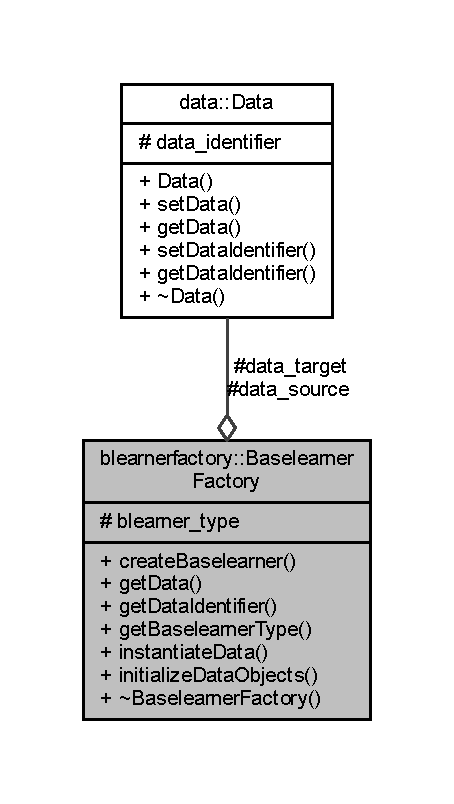
\includegraphics[width=219pt]{classblearnerfactory_1_1_baselearner_factory__coll__graph}
\end{center}
\end{figure}
\subsection*{Public Member Functions}
\begin{DoxyCompactItemize}
\item 
virtual \mbox{\hyperlink{classblearner_1_1_baselearner}{blearner\+::\+Baselearner}} $\ast$ \mbox{\hyperlink{classblearnerfactory_1_1_baselearner_factory_ac3584a20a84834099a15908690b837bb}{create\+Baselearner}} (const std\+::string \&)=0
\item 
std\+::string \mbox{\hyperlink{classblearnerfactory_1_1_baselearner_factory_a40703963bb3fd273b835a99263d9b599}{get\+Data\+Identifier}} () const
\item 
std\+::string \mbox{\hyperlink{classblearnerfactory_1_1_baselearner_factory_a05d5c00f7a434548868c4ad21d0f5fda}{get\+Baselearner\+Type}} () const
\item 
virtual arma\+::mat \mbox{\hyperlink{classblearnerfactory_1_1_baselearner_factory_ac4a38c4815fb33b8d4785745117c5e57}{instantiate\+Data}} (const arma\+::mat \&)=0
\item 
virtual arma\+::mat \mbox{\hyperlink{classblearnerfactory_1_1_baselearner_factory_aa3e4580bca870ca3b742dda6c820e1e6}{get\+Data}} () const =0
\item 
void \mbox{\hyperlink{classblearnerfactory_1_1_baselearner_factory_a147d4ef123ec382fe402d562a91df4d2}{initialize\+Data\+Objects}} (\mbox{\hyperlink{classdata_1_1_data}{data\+::\+Data}} $\ast$, \mbox{\hyperlink{classdata_1_1_data}{data\+::\+Data}} $\ast$)
\item 
virtual \mbox{\hyperlink{classblearnerfactory_1_1_baselearner_factory_adc9d1d3c8fc774c9d856117632c8aadb}{$\sim$\+Baselearner\+Factory}} ()
\end{DoxyCompactItemize}
\subsection*{Protected Attributes}
\begin{DoxyCompactItemize}
\item 
std\+::string \mbox{\hyperlink{classblearnerfactory_1_1_baselearner_factory_a3382b7d9833484f63755a26447a5d2e4}{blearner\+\_\+type}}
\item 
\mbox{\hyperlink{classdata_1_1_data}{data\+::\+Data}} $\ast$ \mbox{\hyperlink{classblearnerfactory_1_1_baselearner_factory_a6194191695958b4035d3ea0841c2320c}{data\+\_\+source}}
\item 
\mbox{\hyperlink{classdata_1_1_data}{data\+::\+Data}} $\ast$ \mbox{\hyperlink{classblearnerfactory_1_1_baselearner_factory_af2cb5c226c90469c6a70b677214ecc2f}{data\+\_\+target}}
\end{DoxyCompactItemize}


\subsection{Constructor \& Destructor Documentation}
\mbox{\Hypertarget{classblearnerfactory_1_1_baselearner_factory_adc9d1d3c8fc774c9d856117632c8aadb}\label{classblearnerfactory_1_1_baselearner_factory_adc9d1d3c8fc774c9d856117632c8aadb}} 
\index{blearnerfactory\+::\+Baselearner\+Factory@{blearnerfactory\+::\+Baselearner\+Factory}!````~Baselearner\+Factory@{$\sim$\+Baselearner\+Factory}}
\index{````~Baselearner\+Factory@{$\sim$\+Baselearner\+Factory}!blearnerfactory\+::\+Baselearner\+Factory@{blearnerfactory\+::\+Baselearner\+Factory}}
\subsubsection{\texorpdfstring{$\sim$\+Baselearner\+Factory()}{~BaselearnerFactory()}}
{\footnotesize\ttfamily blearnerfactory\+::\+Baselearner\+Factory\+::$\sim$\+Baselearner\+Factory (\begin{DoxyParamCaption}{ }\end{DoxyParamCaption})\hspace{0.3cm}{\ttfamily [virtual]}}



\subsection{Member Function Documentation}
\mbox{\Hypertarget{classblearnerfactory_1_1_baselearner_factory_ac3584a20a84834099a15908690b837bb}\label{classblearnerfactory_1_1_baselearner_factory_ac3584a20a84834099a15908690b837bb}} 
\index{blearnerfactory\+::\+Baselearner\+Factory@{blearnerfactory\+::\+Baselearner\+Factory}!create\+Baselearner@{create\+Baselearner}}
\index{create\+Baselearner@{create\+Baselearner}!blearnerfactory\+::\+Baselearner\+Factory@{blearnerfactory\+::\+Baselearner\+Factory}}
\subsubsection{\texorpdfstring{create\+Baselearner()}{createBaselearner()}}
{\footnotesize\ttfamily virtual \mbox{\hyperlink{classblearner_1_1_baselearner}{blearner\+::\+Baselearner}}$\ast$ blearnerfactory\+::\+Baselearner\+Factory\+::create\+Baselearner (\begin{DoxyParamCaption}\item[{const std\+::string \&}]{ }\end{DoxyParamCaption})\hspace{0.3cm}{\ttfamily [pure virtual]}}



Implemented in \mbox{\hyperlink{classblearnerfactory_1_1_baselearner_custom_cpp_factory_a1754f789953cc9d12f7cdd861772d13b}{blearnerfactory\+::\+Baselearner\+Custom\+Cpp\+Factory}}, \mbox{\hyperlink{classblearnerfactory_1_1_baselearner_custom_factory_a79a93fe73bd8f307bb888f76da39246d}{blearnerfactory\+::\+Baselearner\+Custom\+Factory}}, \mbox{\hyperlink{classblearnerfactory_1_1_baselearner_p_spline_factory_a3f47f46766e8e50eafe824bd97f7fc44}{blearnerfactory\+::\+Baselearner\+P\+Spline\+Factory}}, and \mbox{\hyperlink{classblearnerfactory_1_1_baselearner_polynomial_factory_a18095806fa93e6ac2159e966ededc1cf}{blearnerfactory\+::\+Baselearner\+Polynomial\+Factory}}.

\mbox{\Hypertarget{classblearnerfactory_1_1_baselearner_factory_a05d5c00f7a434548868c4ad21d0f5fda}\label{classblearnerfactory_1_1_baselearner_factory_a05d5c00f7a434548868c4ad21d0f5fda}} 
\index{blearnerfactory\+::\+Baselearner\+Factory@{blearnerfactory\+::\+Baselearner\+Factory}!get\+Baselearner\+Type@{get\+Baselearner\+Type}}
\index{get\+Baselearner\+Type@{get\+Baselearner\+Type}!blearnerfactory\+::\+Baselearner\+Factory@{blearnerfactory\+::\+Baselearner\+Factory}}
\subsubsection{\texorpdfstring{get\+Baselearner\+Type()}{getBaselearnerType()}}
{\footnotesize\ttfamily std\+::string blearnerfactory\+::\+Baselearner\+Factory\+::get\+Baselearner\+Type (\begin{DoxyParamCaption}{ }\end{DoxyParamCaption}) const}

\mbox{\Hypertarget{classblearnerfactory_1_1_baselearner_factory_aa3e4580bca870ca3b742dda6c820e1e6}\label{classblearnerfactory_1_1_baselearner_factory_aa3e4580bca870ca3b742dda6c820e1e6}} 
\index{blearnerfactory\+::\+Baselearner\+Factory@{blearnerfactory\+::\+Baselearner\+Factory}!get\+Data@{get\+Data}}
\index{get\+Data@{get\+Data}!blearnerfactory\+::\+Baselearner\+Factory@{blearnerfactory\+::\+Baselearner\+Factory}}
\subsubsection{\texorpdfstring{get\+Data()}{getData()}}
{\footnotesize\ttfamily virtual arma\+::mat blearnerfactory\+::\+Baselearner\+Factory\+::get\+Data (\begin{DoxyParamCaption}{ }\end{DoxyParamCaption}) const\hspace{0.3cm}{\ttfamily [pure virtual]}}



Implemented in \mbox{\hyperlink{classblearnerfactory_1_1_baselearner_custom_cpp_factory_af11e8ca40f235632dba38ed3849f7606}{blearnerfactory\+::\+Baselearner\+Custom\+Cpp\+Factory}}, \mbox{\hyperlink{classblearnerfactory_1_1_baselearner_custom_factory_ae61c7af49c08d61b7714561bde1824d8}{blearnerfactory\+::\+Baselearner\+Custom\+Factory}}, \mbox{\hyperlink{classblearnerfactory_1_1_baselearner_p_spline_factory_a542e3f962314ea7fe46cfe8eed4c4da7}{blearnerfactory\+::\+Baselearner\+P\+Spline\+Factory}}, and \mbox{\hyperlink{classblearnerfactory_1_1_baselearner_polynomial_factory_af6d997c89f2e81a490352f23dee1ef9d}{blearnerfactory\+::\+Baselearner\+Polynomial\+Factory}}.

\mbox{\Hypertarget{classblearnerfactory_1_1_baselearner_factory_a40703963bb3fd273b835a99263d9b599}\label{classblearnerfactory_1_1_baselearner_factory_a40703963bb3fd273b835a99263d9b599}} 
\index{blearnerfactory\+::\+Baselearner\+Factory@{blearnerfactory\+::\+Baselearner\+Factory}!get\+Data\+Identifier@{get\+Data\+Identifier}}
\index{get\+Data\+Identifier@{get\+Data\+Identifier}!blearnerfactory\+::\+Baselearner\+Factory@{blearnerfactory\+::\+Baselearner\+Factory}}
\subsubsection{\texorpdfstring{get\+Data\+Identifier()}{getDataIdentifier()}}
{\footnotesize\ttfamily std\+::string blearnerfactory\+::\+Baselearner\+Factory\+::get\+Data\+Identifier (\begin{DoxyParamCaption}{ }\end{DoxyParamCaption}) const}

Here is the call graph for this function\+:\nopagebreak
\begin{figure}[H]
\begin{center}
\leavevmode
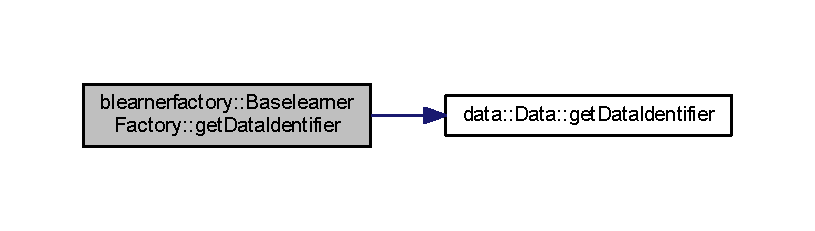
\includegraphics[width=350pt]{classblearnerfactory_1_1_baselearner_factory_a40703963bb3fd273b835a99263d9b599_cgraph}
\end{center}
\end{figure}
Here is the caller graph for this function\+:\nopagebreak
\begin{figure}[H]
\begin{center}
\leavevmode
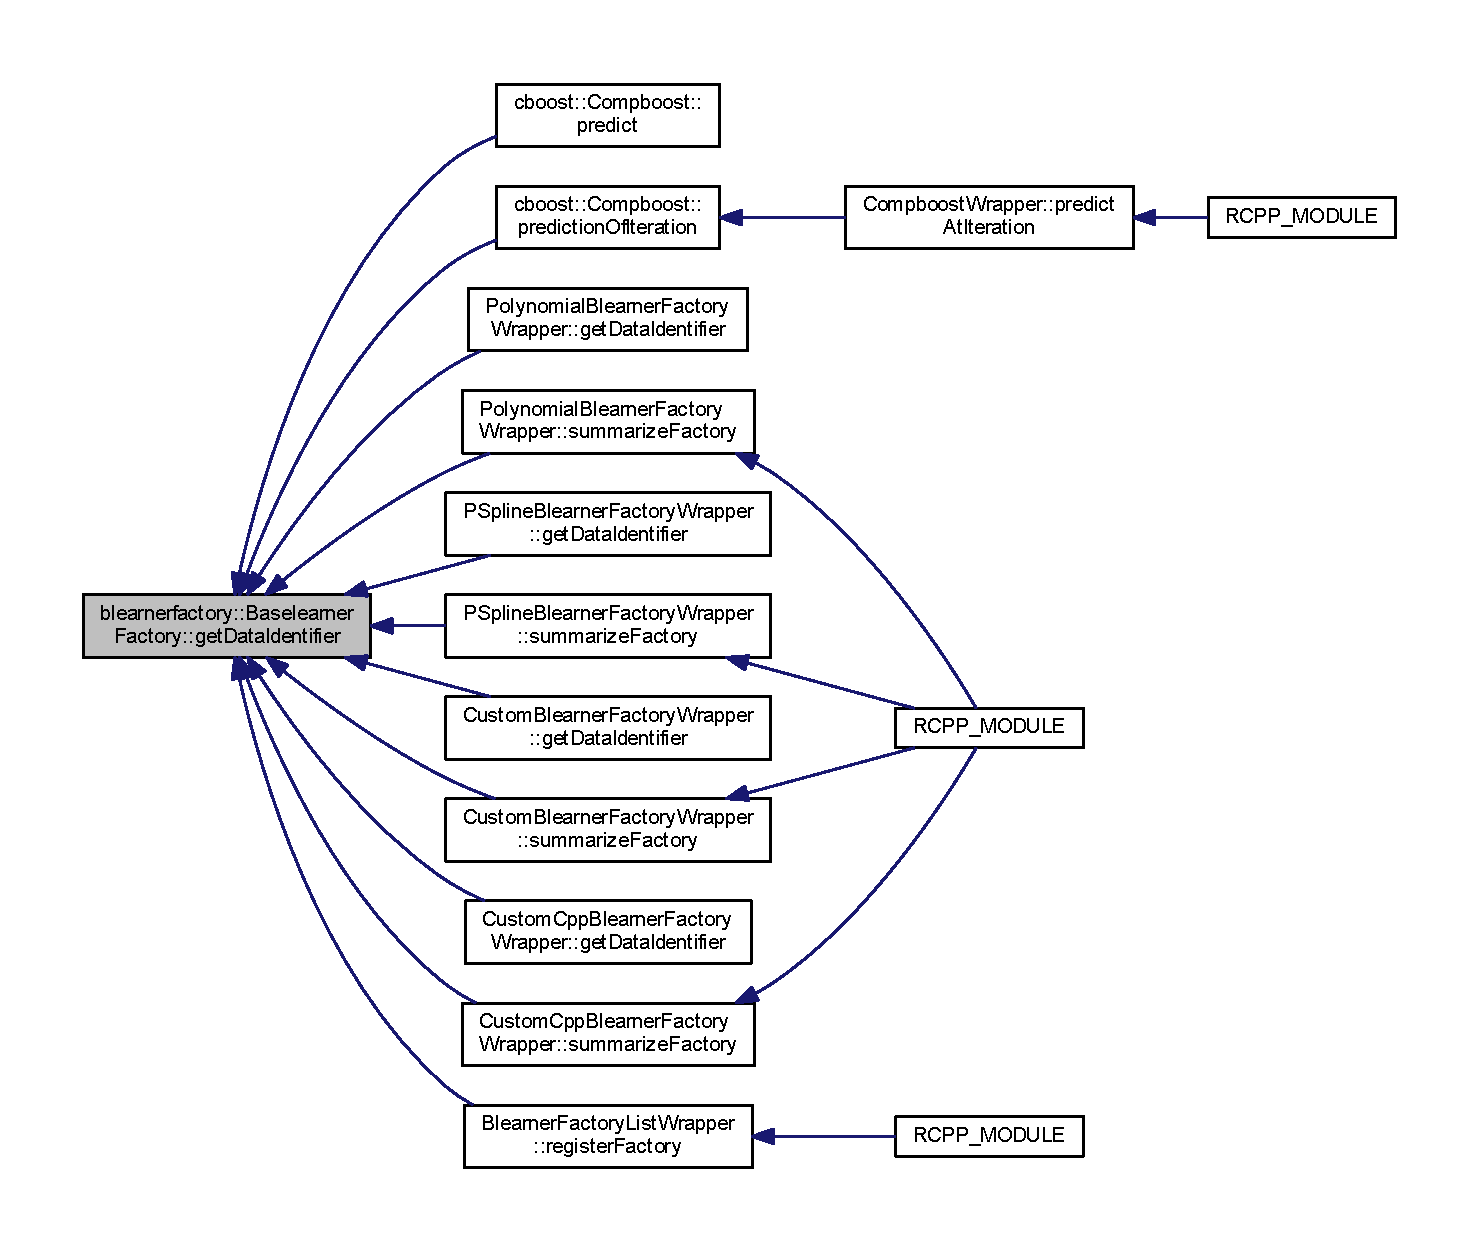
\includegraphics[width=350pt]{classblearnerfactory_1_1_baselearner_factory_a40703963bb3fd273b835a99263d9b599_icgraph}
\end{center}
\end{figure}
\mbox{\Hypertarget{classblearnerfactory_1_1_baselearner_factory_a147d4ef123ec382fe402d562a91df4d2}\label{classblearnerfactory_1_1_baselearner_factory_a147d4ef123ec382fe402d562a91df4d2}} 
\index{blearnerfactory\+::\+Baselearner\+Factory@{blearnerfactory\+::\+Baselearner\+Factory}!initialize\+Data\+Objects@{initialize\+Data\+Objects}}
\index{initialize\+Data\+Objects@{initialize\+Data\+Objects}!blearnerfactory\+::\+Baselearner\+Factory@{blearnerfactory\+::\+Baselearner\+Factory}}
\subsubsection{\texorpdfstring{initialize\+Data\+Objects()}{initializeDataObjects()}}
{\footnotesize\ttfamily void blearnerfactory\+::\+Baselearner\+Factory\+::initialize\+Data\+Objects (\begin{DoxyParamCaption}\item[{\mbox{\hyperlink{classdata_1_1_data}{data\+::\+Data}} $\ast$}]{data\+\_\+source0,  }\item[{\mbox{\hyperlink{classdata_1_1_data}{data\+::\+Data}} $\ast$}]{data\+\_\+target0 }\end{DoxyParamCaption})}

Here is the call graph for this function\+:\nopagebreak
\begin{figure}[H]
\begin{center}
\leavevmode
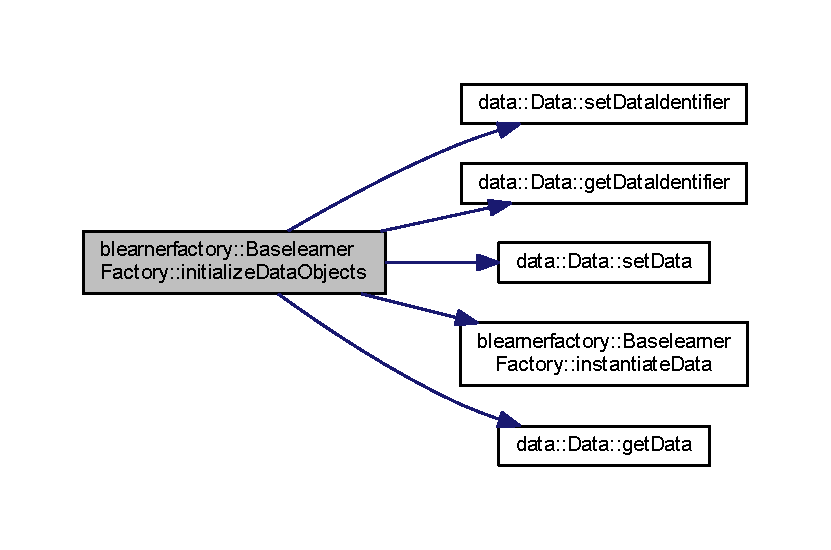
\includegraphics[width=350pt]{classblearnerfactory_1_1_baselearner_factory_a147d4ef123ec382fe402d562a91df4d2_cgraph}
\end{center}
\end{figure}
Here is the caller graph for this function\+:\nopagebreak
\begin{figure}[H]
\begin{center}
\leavevmode
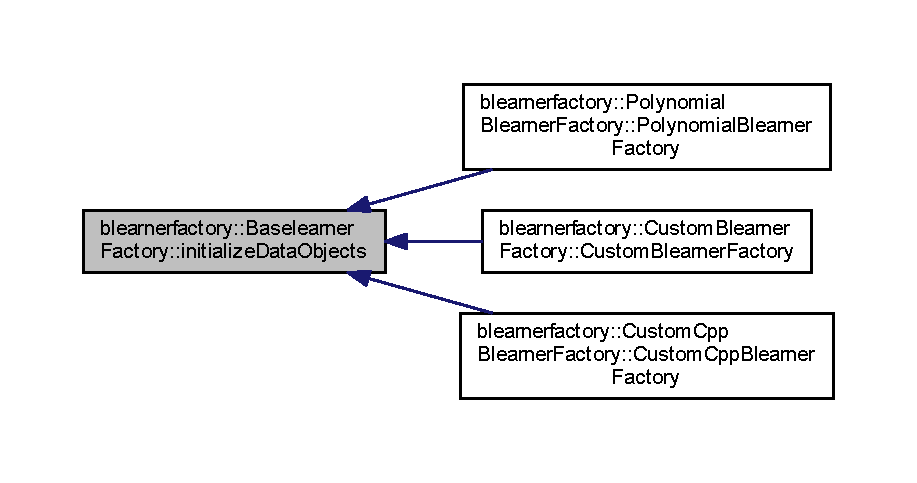
\includegraphics[width=350pt]{classblearnerfactory_1_1_baselearner_factory_a147d4ef123ec382fe402d562a91df4d2_icgraph}
\end{center}
\end{figure}
\mbox{\Hypertarget{classblearnerfactory_1_1_baselearner_factory_ac4a38c4815fb33b8d4785745117c5e57}\label{classblearnerfactory_1_1_baselearner_factory_ac4a38c4815fb33b8d4785745117c5e57}} 
\index{blearnerfactory\+::\+Baselearner\+Factory@{blearnerfactory\+::\+Baselearner\+Factory}!instantiate\+Data@{instantiate\+Data}}
\index{instantiate\+Data@{instantiate\+Data}!blearnerfactory\+::\+Baselearner\+Factory@{blearnerfactory\+::\+Baselearner\+Factory}}
\subsubsection{\texorpdfstring{instantiate\+Data()}{instantiateData()}}
{\footnotesize\ttfamily virtual arma\+::mat blearnerfactory\+::\+Baselearner\+Factory\+::instantiate\+Data (\begin{DoxyParamCaption}\item[{const arma\+::mat \&}]{ }\end{DoxyParamCaption})\hspace{0.3cm}{\ttfamily [pure virtual]}}



Implemented in \mbox{\hyperlink{classblearnerfactory_1_1_baselearner_custom_cpp_factory_a1e7c75381ec018b38efa021ba4dd475f}{blearnerfactory\+::\+Baselearner\+Custom\+Cpp\+Factory}}, \mbox{\hyperlink{classblearnerfactory_1_1_baselearner_custom_factory_ac37e7305a627f98729d266b54cf8fa1c}{blearnerfactory\+::\+Baselearner\+Custom\+Factory}}, \mbox{\hyperlink{classblearnerfactory_1_1_baselearner_p_spline_factory_a8e9f7977906b310d21dda5cceb15c0d8}{blearnerfactory\+::\+Baselearner\+P\+Spline\+Factory}}, and \mbox{\hyperlink{classblearnerfactory_1_1_baselearner_polynomial_factory_ae8a2c70c75eb37e6c782d1bb17627272}{blearnerfactory\+::\+Baselearner\+Polynomial\+Factory}}.

Here is the caller graph for this function\+:\nopagebreak
\begin{figure}[H]
\begin{center}
\leavevmode
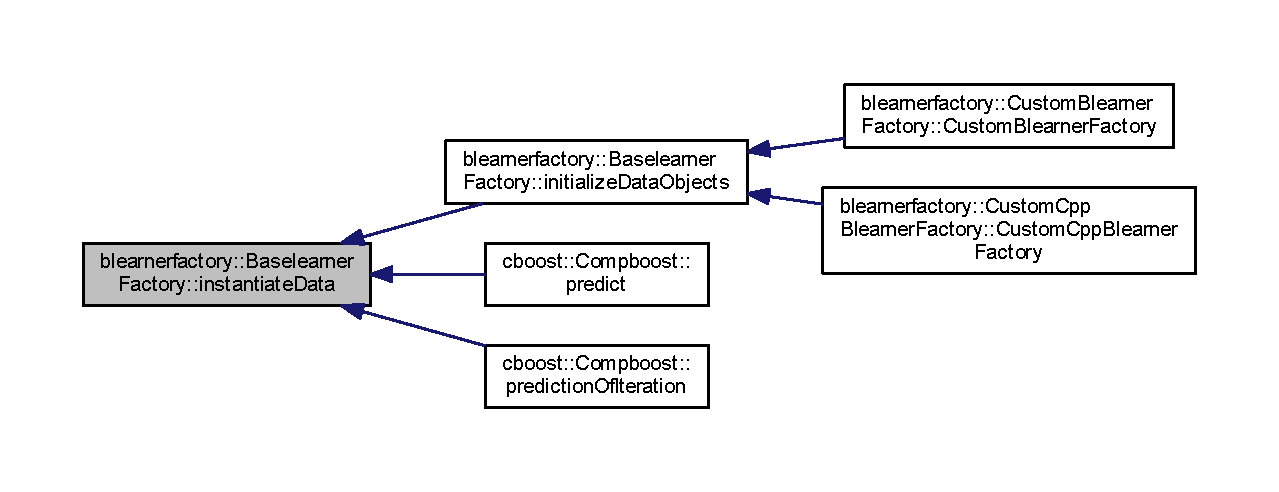
\includegraphics[width=350pt]{classblearnerfactory_1_1_baselearner_factory_ac4a38c4815fb33b8d4785745117c5e57_icgraph}
\end{center}
\end{figure}


\subsection{Member Data Documentation}
\mbox{\Hypertarget{classblearnerfactory_1_1_baselearner_factory_a3382b7d9833484f63755a26447a5d2e4}\label{classblearnerfactory_1_1_baselearner_factory_a3382b7d9833484f63755a26447a5d2e4}} 
\index{blearnerfactory\+::\+Baselearner\+Factory@{blearnerfactory\+::\+Baselearner\+Factory}!blearner\+\_\+type@{blearner\+\_\+type}}
\index{blearner\+\_\+type@{blearner\+\_\+type}!blearnerfactory\+::\+Baselearner\+Factory@{blearnerfactory\+::\+Baselearner\+Factory}}
\subsubsection{\texorpdfstring{blearner\+\_\+type}{blearner\_type}}
{\footnotesize\ttfamily std\+::string blearnerfactory\+::\+Baselearner\+Factory\+::blearner\+\_\+type\hspace{0.3cm}{\ttfamily [protected]}}

\mbox{\Hypertarget{classblearnerfactory_1_1_baselearner_factory_a6194191695958b4035d3ea0841c2320c}\label{classblearnerfactory_1_1_baselearner_factory_a6194191695958b4035d3ea0841c2320c}} 
\index{blearnerfactory\+::\+Baselearner\+Factory@{blearnerfactory\+::\+Baselearner\+Factory}!data\+\_\+source@{data\+\_\+source}}
\index{data\+\_\+source@{data\+\_\+source}!blearnerfactory\+::\+Baselearner\+Factory@{blearnerfactory\+::\+Baselearner\+Factory}}
\subsubsection{\texorpdfstring{data\+\_\+source}{data\_source}}
{\footnotesize\ttfamily \mbox{\hyperlink{classdata_1_1_data}{data\+::\+Data}}$\ast$ blearnerfactory\+::\+Baselearner\+Factory\+::data\+\_\+source\hspace{0.3cm}{\ttfamily [protected]}}

\mbox{\Hypertarget{classblearnerfactory_1_1_baselearner_factory_af2cb5c226c90469c6a70b677214ecc2f}\label{classblearnerfactory_1_1_baselearner_factory_af2cb5c226c90469c6a70b677214ecc2f}} 
\index{blearnerfactory\+::\+Baselearner\+Factory@{blearnerfactory\+::\+Baselearner\+Factory}!data\+\_\+target@{data\+\_\+target}}
\index{data\+\_\+target@{data\+\_\+target}!blearnerfactory\+::\+Baselearner\+Factory@{blearnerfactory\+::\+Baselearner\+Factory}}
\subsubsection{\texorpdfstring{data\+\_\+target}{data\_target}}
{\footnotesize\ttfamily \mbox{\hyperlink{classdata_1_1_data}{data\+::\+Data}}$\ast$ blearnerfactory\+::\+Baselearner\+Factory\+::data\+\_\+target\hspace{0.3cm}{\ttfamily [protected]}}



The documentation for this class was generated from the following files\+:\begin{DoxyCompactItemize}
\item 
C\+:/\+Users/schal/\+One\+Drive/github\+\_\+repos/compboost/src/\mbox{\hyperlink{baselearner__factory_8h}{baselearner\+\_\+factory.\+h}}\item 
C\+:/\+Users/schal/\+One\+Drive/github\+\_\+repos/compboost/src/\mbox{\hyperlink{baselearner__factory_8cpp}{baselearner\+\_\+factory.\+cpp}}\end{DoxyCompactItemize}

\hypertarget{classblearnerlist_1_1_baselearner_factory_list}{}\section{blearnerlist\+:\+:Baselearner\+Factory\+List Class Reference}
\label{classblearnerlist_1_1_baselearner_factory_list}\index{blearnerlist\+::\+Baselearner\+Factory\+List@{blearnerlist\+::\+Baselearner\+Factory\+List}}


{\ttfamily \#include $<$baselearner\+\_\+factory\+\_\+list.\+h$>$}



Collaboration diagram for blearnerlist\+:\+:Baselearner\+Factory\+List\+:\nopagebreak
\begin{figure}[H]
\begin{center}
\leavevmode
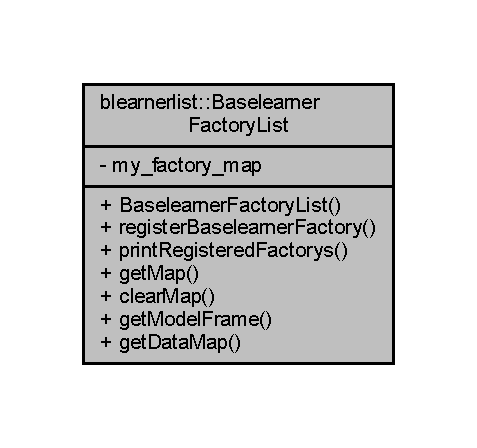
\includegraphics[width=229pt]{classblearnerlist_1_1_baselearner_factory_list__coll__graph}
\end{center}
\end{figure}
\subsection*{Public Member Functions}
\begin{DoxyCompactItemize}
\item 
\hyperlink{classblearnerlist_1_1_baselearner_factory_list_a438e2cfeecfdecaff27624225819f99b}{Baselearner\+Factory\+List} ()
\item 
void \hyperlink{classblearnerlist_1_1_baselearner_factory_list_a6f5d8eb26f5f5ae4856d62eb9d649f4f}{register\+Baselearner\+Factory} (const std\+::string \&, \hyperlink{classblearnerfactory_1_1_baselearner_factory}{blearnerfactory\+::\+Baselearner\+Factory} $\ast$)
\item 
void \hyperlink{classblearnerlist_1_1_baselearner_factory_list_a1d0242c96044f78c448183ed4a97e079}{print\+Registered\+Factorys} () const
\item 
\hyperlink{baselearner__factory__list_8h_a058570e00ae11b882cfed36eb40be025}{blearner\+\_\+factory\+\_\+map} \hyperlink{classblearnerlist_1_1_baselearner_factory_list_aeb573190a689af611e2f80ca8ed65d95}{get\+Map} () const
\item 
void \hyperlink{classblearnerlist_1_1_baselearner_factory_list_aacbe97968ca672d2481d5f8dce0bbf94}{clear\+Map} ()
\item 
std\+::pair$<$ std\+::vector$<$ std\+::string $>$, arma\+::mat $>$ \hyperlink{classblearnerlist_1_1_baselearner_factory_list_a1f0d601a978c0f50cf9b6228c1f92ce8}{get\+Model\+Frame} () const
\item 
std\+::map$<$ std\+::string, arma\+::mat $>$ \hyperlink{classblearnerlist_1_1_baselearner_factory_list_aeb83b67769e5fb34e7acc14c7e651dfc}{get\+Data\+Map} () const
\end{DoxyCompactItemize}
\subsection*{Private Attributes}
\begin{DoxyCompactItemize}
\item 
\hyperlink{baselearner__factory__list_8h_a058570e00ae11b882cfed36eb40be025}{blearner\+\_\+factory\+\_\+map} \hyperlink{classblearnerlist_1_1_baselearner_factory_list_a839e9b3f1bf73e995c35f7a6d0f64113}{my\+\_\+factory\+\_\+map}
\end{DoxyCompactItemize}


\subsection{Constructor \& Destructor Documentation}
\mbox{\Hypertarget{classblearnerlist_1_1_baselearner_factory_list_a438e2cfeecfdecaff27624225819f99b}\label{classblearnerlist_1_1_baselearner_factory_list_a438e2cfeecfdecaff27624225819f99b}} 
\index{blearnerlist\+::\+Baselearner\+Factory\+List@{blearnerlist\+::\+Baselearner\+Factory\+List}!Baselearner\+Factory\+List@{Baselearner\+Factory\+List}}
\index{Baselearner\+Factory\+List@{Baselearner\+Factory\+List}!blearnerlist\+::\+Baselearner\+Factory\+List@{blearnerlist\+::\+Baselearner\+Factory\+List}}
\subsubsection{\texorpdfstring{Baselearner\+Factory\+List()}{BaselearnerFactoryList()}}
{\footnotesize\ttfamily blearnerlist\+::\+Baselearner\+Factory\+List\+::\+Baselearner\+Factory\+List (\begin{DoxyParamCaption}{ }\end{DoxyParamCaption})}



\subsection{Member Function Documentation}
\mbox{\Hypertarget{classblearnerlist_1_1_baselearner_factory_list_aacbe97968ca672d2481d5f8dce0bbf94}\label{classblearnerlist_1_1_baselearner_factory_list_aacbe97968ca672d2481d5f8dce0bbf94}} 
\index{blearnerlist\+::\+Baselearner\+Factory\+List@{blearnerlist\+::\+Baselearner\+Factory\+List}!clear\+Map@{clear\+Map}}
\index{clear\+Map@{clear\+Map}!blearnerlist\+::\+Baselearner\+Factory\+List@{blearnerlist\+::\+Baselearner\+Factory\+List}}
\subsubsection{\texorpdfstring{clear\+Map()}{clearMap()}}
{\footnotesize\ttfamily void blearnerlist\+::\+Baselearner\+Factory\+List\+::clear\+Map (\begin{DoxyParamCaption}{ }\end{DoxyParamCaption})}

\mbox{\Hypertarget{classblearnerlist_1_1_baselearner_factory_list_aeb83b67769e5fb34e7acc14c7e651dfc}\label{classblearnerlist_1_1_baselearner_factory_list_aeb83b67769e5fb34e7acc14c7e651dfc}} 
\index{blearnerlist\+::\+Baselearner\+Factory\+List@{blearnerlist\+::\+Baselearner\+Factory\+List}!get\+Data\+Map@{get\+Data\+Map}}
\index{get\+Data\+Map@{get\+Data\+Map}!blearnerlist\+::\+Baselearner\+Factory\+List@{blearnerlist\+::\+Baselearner\+Factory\+List}}
\subsubsection{\texorpdfstring{get\+Data\+Map()}{getDataMap()}}
{\footnotesize\ttfamily std\+::map$<$ std\+::string, arma\+::mat $>$ blearnerlist\+::\+Baselearner\+Factory\+List\+::get\+Data\+Map (\begin{DoxyParamCaption}{ }\end{DoxyParamCaption}) const}

Here is the caller graph for this function\+:\nopagebreak
\begin{figure}[H]
\begin{center}
\leavevmode
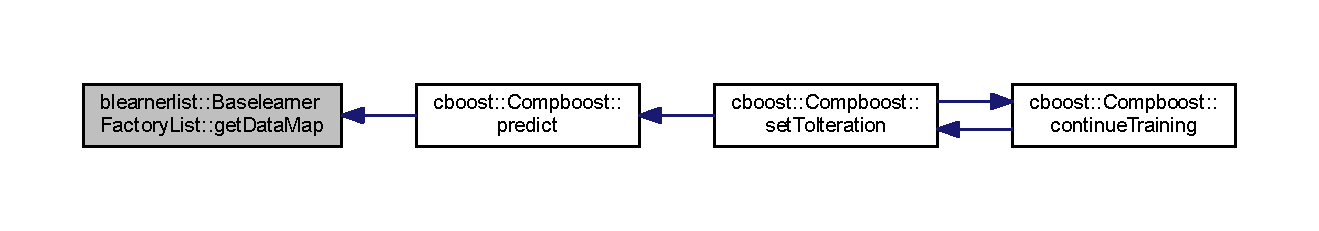
\includegraphics[width=350pt]{classblearnerlist_1_1_baselearner_factory_list_aeb83b67769e5fb34e7acc14c7e651dfc_icgraph}
\end{center}
\end{figure}
\mbox{\Hypertarget{classblearnerlist_1_1_baselearner_factory_list_aeb573190a689af611e2f80ca8ed65d95}\label{classblearnerlist_1_1_baselearner_factory_list_aeb573190a689af611e2f80ca8ed65d95}} 
\index{blearnerlist\+::\+Baselearner\+Factory\+List@{blearnerlist\+::\+Baselearner\+Factory\+List}!get\+Map@{get\+Map}}
\index{get\+Map@{get\+Map}!blearnerlist\+::\+Baselearner\+Factory\+List@{blearnerlist\+::\+Baselearner\+Factory\+List}}
\subsubsection{\texorpdfstring{get\+Map()}{getMap()}}
{\footnotesize\ttfamily \hyperlink{baselearner__factory__list_8h_a058570e00ae11b882cfed36eb40be025}{blearner\+\_\+factory\+\_\+map} blearnerlist\+::\+Baselearner\+Factory\+List\+::get\+Map (\begin{DoxyParamCaption}{ }\end{DoxyParamCaption}) const}

Here is the caller graph for this function\+:\nopagebreak
\begin{figure}[H]
\begin{center}
\leavevmode
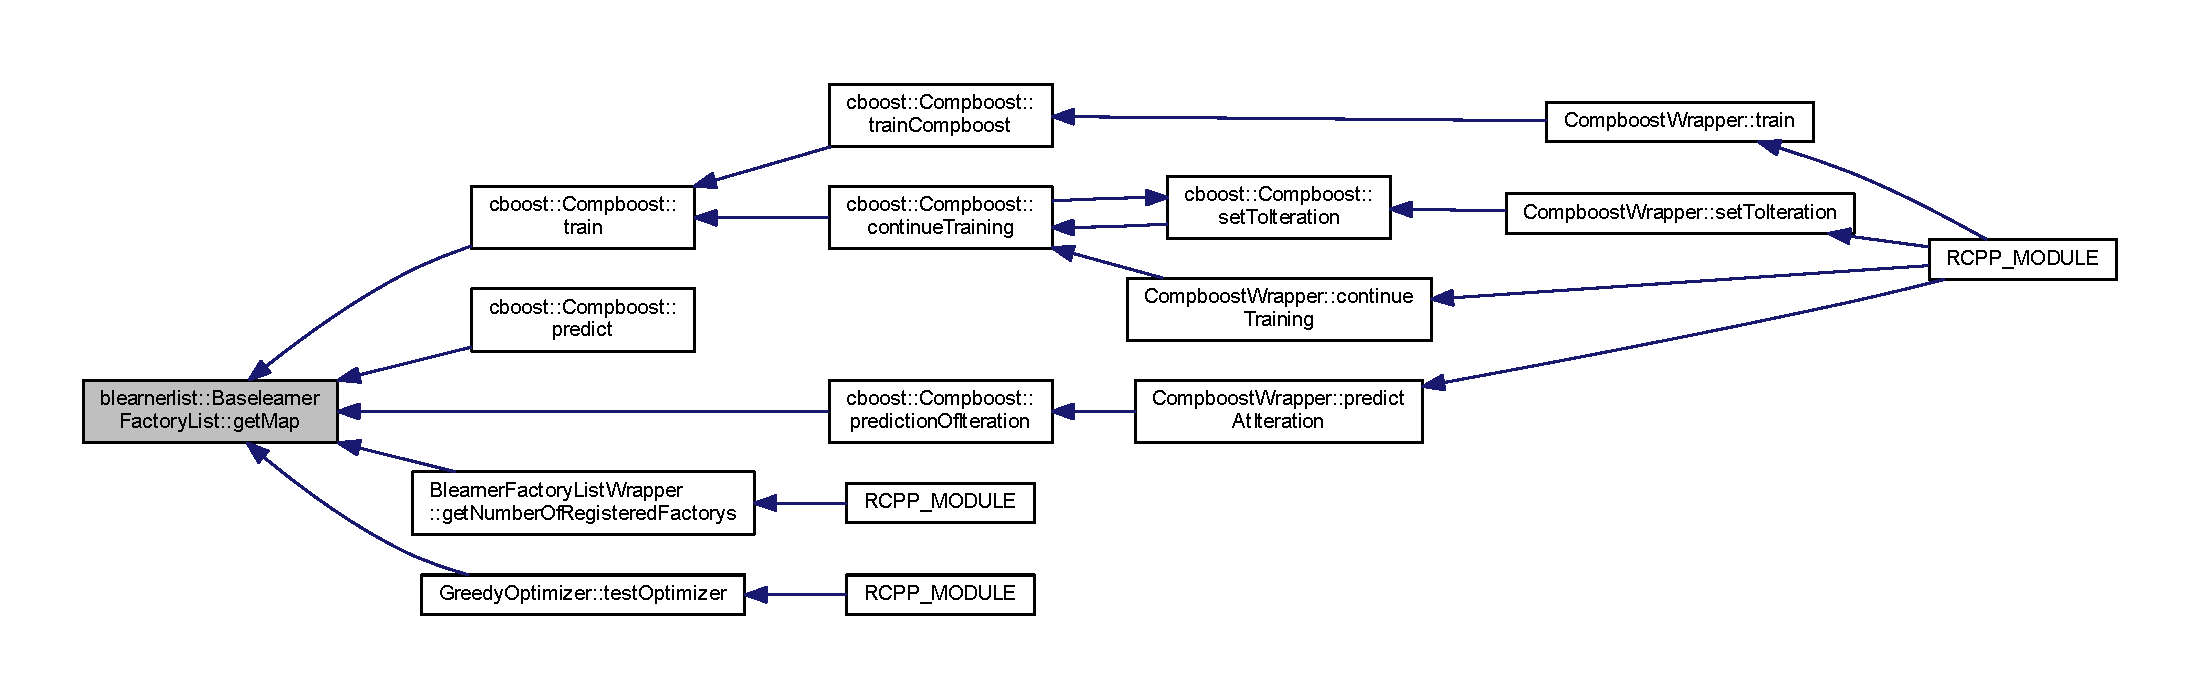
\includegraphics[width=350pt]{classblearnerlist_1_1_baselearner_factory_list_aeb573190a689af611e2f80ca8ed65d95_icgraph}
\end{center}
\end{figure}
\mbox{\Hypertarget{classblearnerlist_1_1_baselearner_factory_list_a1f0d601a978c0f50cf9b6228c1f92ce8}\label{classblearnerlist_1_1_baselearner_factory_list_a1f0d601a978c0f50cf9b6228c1f92ce8}} 
\index{blearnerlist\+::\+Baselearner\+Factory\+List@{blearnerlist\+::\+Baselearner\+Factory\+List}!get\+Model\+Frame@{get\+Model\+Frame}}
\index{get\+Model\+Frame@{get\+Model\+Frame}!blearnerlist\+::\+Baselearner\+Factory\+List@{blearnerlist\+::\+Baselearner\+Factory\+List}}
\subsubsection{\texorpdfstring{get\+Model\+Frame()}{getModelFrame()}}
{\footnotesize\ttfamily std\+::pair$<$ std\+::vector$<$ std\+::string $>$, arma\+::mat $>$ blearnerlist\+::\+Baselearner\+Factory\+List\+::get\+Model\+Frame (\begin{DoxyParamCaption}{ }\end{DoxyParamCaption}) const}

\mbox{\Hypertarget{classblearnerlist_1_1_baselearner_factory_list_a1d0242c96044f78c448183ed4a97e079}\label{classblearnerlist_1_1_baselearner_factory_list_a1d0242c96044f78c448183ed4a97e079}} 
\index{blearnerlist\+::\+Baselearner\+Factory\+List@{blearnerlist\+::\+Baselearner\+Factory\+List}!print\+Registered\+Factorys@{print\+Registered\+Factorys}}
\index{print\+Registered\+Factorys@{print\+Registered\+Factorys}!blearnerlist\+::\+Baselearner\+Factory\+List@{blearnerlist\+::\+Baselearner\+Factory\+List}}
\subsubsection{\texorpdfstring{print\+Registered\+Factorys()}{printRegisteredFactorys()}}
{\footnotesize\ttfamily void blearnerlist\+::\+Baselearner\+Factory\+List\+::print\+Registered\+Factorys (\begin{DoxyParamCaption}{ }\end{DoxyParamCaption}) const}

\mbox{\Hypertarget{classblearnerlist_1_1_baselearner_factory_list_a6f5d8eb26f5f5ae4856d62eb9d649f4f}\label{classblearnerlist_1_1_baselearner_factory_list_a6f5d8eb26f5f5ae4856d62eb9d649f4f}} 
\index{blearnerlist\+::\+Baselearner\+Factory\+List@{blearnerlist\+::\+Baselearner\+Factory\+List}!register\+Baselearner\+Factory@{register\+Baselearner\+Factory}}
\index{register\+Baselearner\+Factory@{register\+Baselearner\+Factory}!blearnerlist\+::\+Baselearner\+Factory\+List@{blearnerlist\+::\+Baselearner\+Factory\+List}}
\subsubsection{\texorpdfstring{register\+Baselearner\+Factory()}{registerBaselearnerFactory()}}
{\footnotesize\ttfamily void blearnerlist\+::\+Baselearner\+Factory\+List\+::register\+Baselearner\+Factory (\begin{DoxyParamCaption}\item[{const std\+::string \&}]{factory\+\_\+id,  }\item[{\hyperlink{classblearnerfactory_1_1_baselearner_factory}{blearnerfactory\+::\+Baselearner\+Factory} $\ast$}]{blearner\+\_\+factory }\end{DoxyParamCaption})}



\subsection{Member Data Documentation}
\mbox{\Hypertarget{classblearnerlist_1_1_baselearner_factory_list_a839e9b3f1bf73e995c35f7a6d0f64113}\label{classblearnerlist_1_1_baselearner_factory_list_a839e9b3f1bf73e995c35f7a6d0f64113}} 
\index{blearnerlist\+::\+Baselearner\+Factory\+List@{blearnerlist\+::\+Baselearner\+Factory\+List}!my\+\_\+factory\+\_\+map@{my\+\_\+factory\+\_\+map}}
\index{my\+\_\+factory\+\_\+map@{my\+\_\+factory\+\_\+map}!blearnerlist\+::\+Baselearner\+Factory\+List@{blearnerlist\+::\+Baselearner\+Factory\+List}}
\subsubsection{\texorpdfstring{my\+\_\+factory\+\_\+map}{my\_factory\_map}}
{\footnotesize\ttfamily \hyperlink{baselearner__factory__list_8h_a058570e00ae11b882cfed36eb40be025}{blearner\+\_\+factory\+\_\+map} blearnerlist\+::\+Baselearner\+Factory\+List\+::my\+\_\+factory\+\_\+map\hspace{0.3cm}{\ttfamily [private]}}



The documentation for this class was generated from the following files\+:\begin{DoxyCompactItemize}
\item 
/home/daniel/github\+\_\+repos/compboost/src/\hyperlink{baselearner__factory__list_8h}{baselearner\+\_\+factory\+\_\+list.\+h}\item 
/home/daniel/github\+\_\+repos/compboost/src/\hyperlink{baselearner__factory__list_8cpp}{baselearner\+\_\+factory\+\_\+list.\+cpp}\end{DoxyCompactItemize}

\hypertarget{classblearnertrack_1_1_baselearner_track}{}\section{blearnertrack\+:\+:Baselearner\+Track Class Reference}
\label{classblearnertrack_1_1_baselearner_track}\index{blearnertrack\+::\+Baselearner\+Track@{blearnertrack\+::\+Baselearner\+Track}}


{\ttfamily \#include $<$baselearner\+\_\+track.\+h$>$}



Collaboration diagram for blearnertrack\+:\+:Baselearner\+Track\+:\nopagebreak
\begin{figure}[H]
\begin{center}
\leavevmode
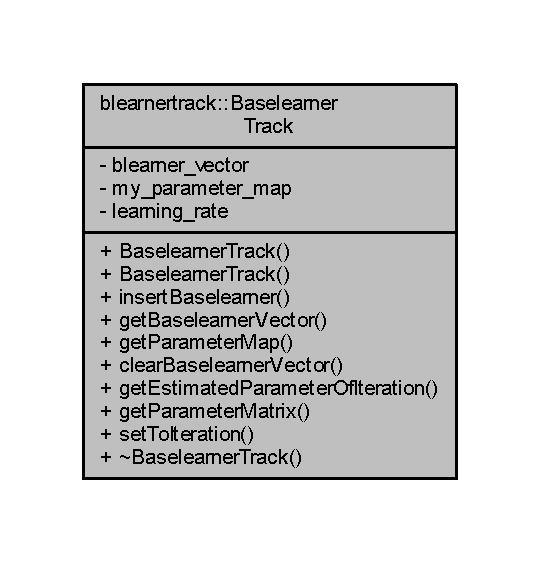
\includegraphics[width=259pt]{classblearnertrack_1_1_baselearner_track__coll__graph}
\end{center}
\end{figure}
\subsection*{Public Member Functions}
\begin{DoxyCompactItemize}
\item 
\mbox{\hyperlink{classblearnertrack_1_1_baselearner_track_ad90a0f286fab221aa2f2ed6401861187}{Baselearner\+Track}} ()
\item 
\mbox{\hyperlink{classblearnertrack_1_1_baselearner_track_aaba614b8351a3e5401d3f924059efc65}{Baselearner\+Track}} (double)
\item 
void \mbox{\hyperlink{classblearnertrack_1_1_baselearner_track_abc5f42093449e665b5b0dfeee8570953}{insert\+Baselearner}} (\mbox{\hyperlink{classblearner_1_1_baselearner}{blearner\+::\+Baselearner}} $\ast$)
\item 
std\+::vector$<$ \mbox{\hyperlink{classblearner_1_1_baselearner}{blearner\+::\+Baselearner}} $\ast$ $>$ \mbox{\hyperlink{classblearnertrack_1_1_baselearner_track_a596429982bd5fb1c8ffabc5f93849235}{get\+Baselearner\+Vector}} () const
\item 
std\+::map$<$ std\+::string, arma\+::mat $>$ \mbox{\hyperlink{classblearnertrack_1_1_baselearner_track_a0ba8e3943b998b58375b892f40f12c73}{get\+Parameter\+Map}} () const
\item 
void \mbox{\hyperlink{classblearnertrack_1_1_baselearner_track_aa178f9d817a01240b6f39075f1f445f2}{clear\+Baselearner\+Vector}} ()
\item 
std\+::map$<$ std\+::string, arma\+::mat $>$ \mbox{\hyperlink{classblearnertrack_1_1_baselearner_track_a9b0678ef3573206959be2068d115c556}{get\+Estimated\+Parameter\+Of\+Iteration}} (const unsigned int \&) const
\item 
std\+::pair$<$ std\+::vector$<$ std\+::string $>$, arma\+::mat $>$ \mbox{\hyperlink{classblearnertrack_1_1_baselearner_track_a4b6d2d8b585148c71ed5b6055c9ab08c}{get\+Parameter\+Matrix}} () const
\item 
void \mbox{\hyperlink{classblearnertrack_1_1_baselearner_track_a06f0ac986a158eecddce64e6c7af0750}{set\+To\+Iteration}} (const unsigned int \&)
\item 
\mbox{\hyperlink{classblearnertrack_1_1_baselearner_track_a93e9a1268d46808b9d6fe768fa11e22a}{$\sim$\+Baselearner\+Track}} ()
\end{DoxyCompactItemize}
\subsection*{Private Attributes}
\begin{DoxyCompactItemize}
\item 
std\+::vector$<$ \mbox{\hyperlink{classblearner_1_1_baselearner}{blearner\+::\+Baselearner}} $\ast$ $>$ \mbox{\hyperlink{classblearnertrack_1_1_baselearner_track_ad37a3a99c04778146256e50c44f2a292}{blearner\+\_\+vector}}
\item 
std\+::map$<$ std\+::string, arma\+::mat $>$ \mbox{\hyperlink{classblearnertrack_1_1_baselearner_track_a3725470c87e28ea32d4b184f1e6aad39}{my\+\_\+parameter\+\_\+map}}
\item 
double \mbox{\hyperlink{classblearnertrack_1_1_baselearner_track_a62d743fe6171c52410e2f5da3dc58ffb}{learning\+\_\+rate}}
\end{DoxyCompactItemize}


\subsection{Constructor \& Destructor Documentation}
\mbox{\Hypertarget{classblearnertrack_1_1_baselearner_track_ad90a0f286fab221aa2f2ed6401861187}\label{classblearnertrack_1_1_baselearner_track_ad90a0f286fab221aa2f2ed6401861187}} 
\index{blearnertrack\+::\+Baselearner\+Track@{blearnertrack\+::\+Baselearner\+Track}!Baselearner\+Track@{Baselearner\+Track}}
\index{Baselearner\+Track@{Baselearner\+Track}!blearnertrack\+::\+Baselearner\+Track@{blearnertrack\+::\+Baselearner\+Track}}
\subsubsection{\texorpdfstring{Baselearner\+Track()}{BaselearnerTrack()}\hspace{0.1cm}{\footnotesize\ttfamily [1/2]}}
{\footnotesize\ttfamily blearnertrack\+::\+Baselearner\+Track\+::\+Baselearner\+Track (\begin{DoxyParamCaption}{ }\end{DoxyParamCaption})}

\mbox{\Hypertarget{classblearnertrack_1_1_baselearner_track_aaba614b8351a3e5401d3f924059efc65}\label{classblearnertrack_1_1_baselearner_track_aaba614b8351a3e5401d3f924059efc65}} 
\index{blearnertrack\+::\+Baselearner\+Track@{blearnertrack\+::\+Baselearner\+Track}!Baselearner\+Track@{Baselearner\+Track}}
\index{Baselearner\+Track@{Baselearner\+Track}!blearnertrack\+::\+Baselearner\+Track@{blearnertrack\+::\+Baselearner\+Track}}
\subsubsection{\texorpdfstring{Baselearner\+Track()}{BaselearnerTrack()}\hspace{0.1cm}{\footnotesize\ttfamily [2/2]}}
{\footnotesize\ttfamily blearnertrack\+::\+Baselearner\+Track\+::\+Baselearner\+Track (\begin{DoxyParamCaption}\item[{double}]{learning\+\_\+rate }\end{DoxyParamCaption})}

\mbox{\Hypertarget{classblearnertrack_1_1_baselearner_track_a93e9a1268d46808b9d6fe768fa11e22a}\label{classblearnertrack_1_1_baselearner_track_a93e9a1268d46808b9d6fe768fa11e22a}} 
\index{blearnertrack\+::\+Baselearner\+Track@{blearnertrack\+::\+Baselearner\+Track}!````~Baselearner\+Track@{$\sim$\+Baselearner\+Track}}
\index{````~Baselearner\+Track@{$\sim$\+Baselearner\+Track}!blearnertrack\+::\+Baselearner\+Track@{blearnertrack\+::\+Baselearner\+Track}}
\subsubsection{\texorpdfstring{$\sim$\+Baselearner\+Track()}{~BaselearnerTrack()}}
{\footnotesize\ttfamily blearnertrack\+::\+Baselearner\+Track\+::$\sim$\+Baselearner\+Track (\begin{DoxyParamCaption}{ }\end{DoxyParamCaption})}

Here is the call graph for this function\+:\nopagebreak
\begin{figure}[H]
\begin{center}
\leavevmode
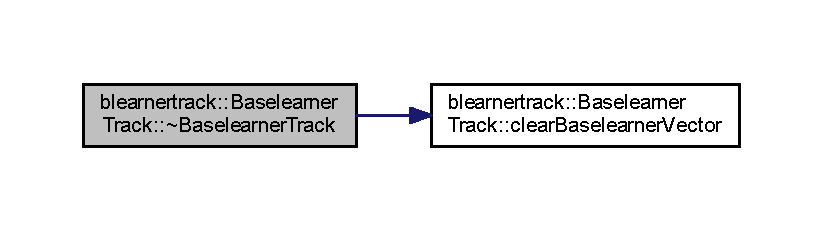
\includegraphics[width=350pt]{classblearnertrack_1_1_baselearner_track_a93e9a1268d46808b9d6fe768fa11e22a_cgraph}
\end{center}
\end{figure}


\subsection{Member Function Documentation}
\mbox{\Hypertarget{classblearnertrack_1_1_baselearner_track_aa178f9d817a01240b6f39075f1f445f2}\label{classblearnertrack_1_1_baselearner_track_aa178f9d817a01240b6f39075f1f445f2}} 
\index{blearnertrack\+::\+Baselearner\+Track@{blearnertrack\+::\+Baselearner\+Track}!clear\+Baselearner\+Vector@{clear\+Baselearner\+Vector}}
\index{clear\+Baselearner\+Vector@{clear\+Baselearner\+Vector}!blearnertrack\+::\+Baselearner\+Track@{blearnertrack\+::\+Baselearner\+Track}}
\subsubsection{\texorpdfstring{clear\+Baselearner\+Vector()}{clearBaselearnerVector()}}
{\footnotesize\ttfamily void blearnertrack\+::\+Baselearner\+Track\+::clear\+Baselearner\+Vector (\begin{DoxyParamCaption}{ }\end{DoxyParamCaption})}

Here is the caller graph for this function\+:\nopagebreak
\begin{figure}[H]
\begin{center}
\leavevmode
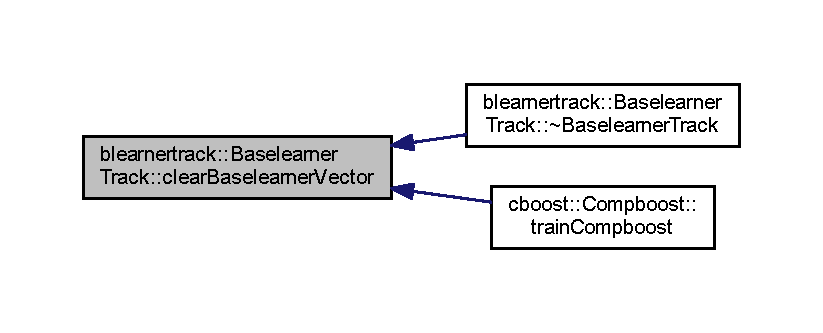
\includegraphics[width=350pt]{classblearnertrack_1_1_baselearner_track_aa178f9d817a01240b6f39075f1f445f2_icgraph}
\end{center}
\end{figure}
\mbox{\Hypertarget{classblearnertrack_1_1_baselearner_track_a596429982bd5fb1c8ffabc5f93849235}\label{classblearnertrack_1_1_baselearner_track_a596429982bd5fb1c8ffabc5f93849235}} 
\index{blearnertrack\+::\+Baselearner\+Track@{blearnertrack\+::\+Baselearner\+Track}!get\+Baselearner\+Vector@{get\+Baselearner\+Vector}}
\index{get\+Baselearner\+Vector@{get\+Baselearner\+Vector}!blearnertrack\+::\+Baselearner\+Track@{blearnertrack\+::\+Baselearner\+Track}}
\subsubsection{\texorpdfstring{get\+Baselearner\+Vector()}{getBaselearnerVector()}}
{\footnotesize\ttfamily std\+::vector$<$ \mbox{\hyperlink{classblearner_1_1_baselearner}{blearner\+::\+Baselearner}} $\ast$ $>$ blearnertrack\+::\+Baselearner\+Track\+::get\+Baselearner\+Vector (\begin{DoxyParamCaption}{ }\end{DoxyParamCaption}) const}

Here is the caller graph for this function\+:\nopagebreak
\begin{figure}[H]
\begin{center}
\leavevmode
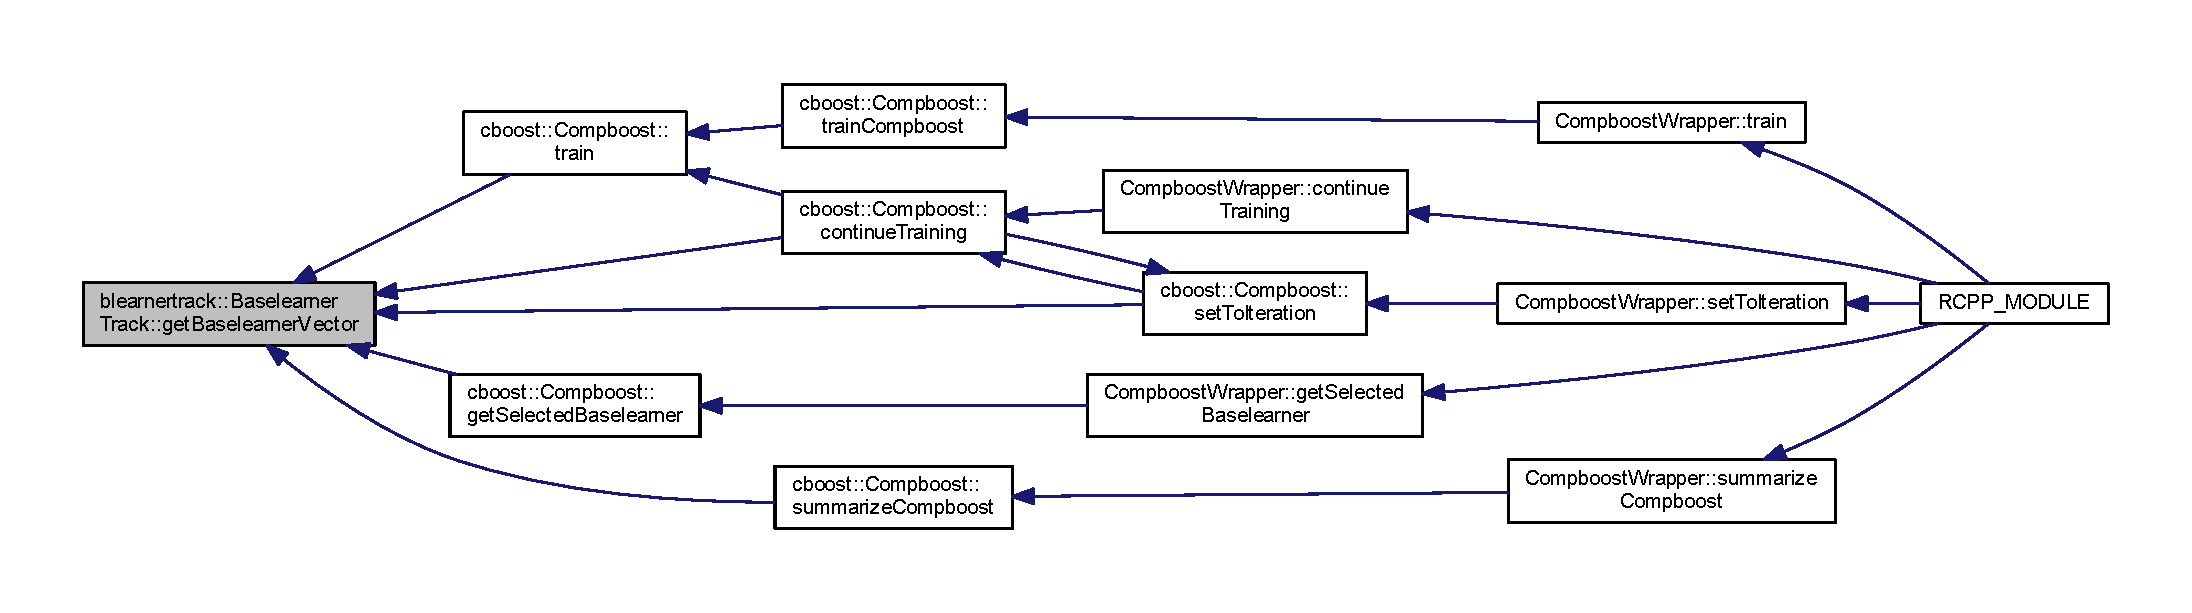
\includegraphics[width=350pt]{classblearnertrack_1_1_baselearner_track_a596429982bd5fb1c8ffabc5f93849235_icgraph}
\end{center}
\end{figure}
\mbox{\Hypertarget{classblearnertrack_1_1_baselearner_track_a9b0678ef3573206959be2068d115c556}\label{classblearnertrack_1_1_baselearner_track_a9b0678ef3573206959be2068d115c556}} 
\index{blearnertrack\+::\+Baselearner\+Track@{blearnertrack\+::\+Baselearner\+Track}!get\+Estimated\+Parameter\+Of\+Iteration@{get\+Estimated\+Parameter\+Of\+Iteration}}
\index{get\+Estimated\+Parameter\+Of\+Iteration@{get\+Estimated\+Parameter\+Of\+Iteration}!blearnertrack\+::\+Baselearner\+Track@{blearnertrack\+::\+Baselearner\+Track}}
\subsubsection{\texorpdfstring{get\+Estimated\+Parameter\+Of\+Iteration()}{getEstimatedParameterOfIteration()}}
{\footnotesize\ttfamily std\+::map$<$ std\+::string, arma\+::mat $>$ blearnertrack\+::\+Baselearner\+Track\+::get\+Estimated\+Parameter\+Of\+Iteration (\begin{DoxyParamCaption}\item[{const unsigned int \&}]{k }\end{DoxyParamCaption}) const}

Here is the caller graph for this function\+:\nopagebreak
\begin{figure}[H]
\begin{center}
\leavevmode
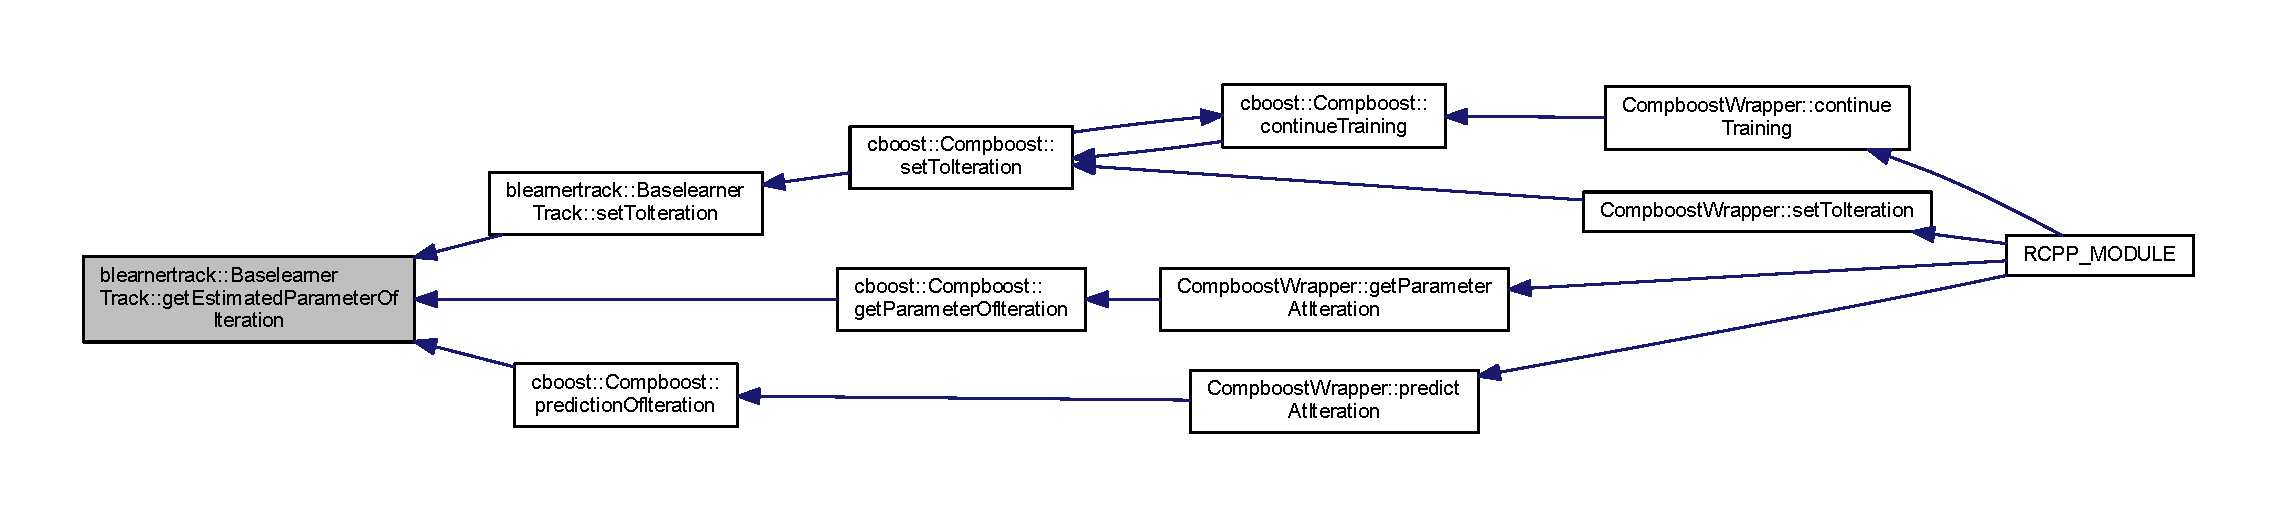
\includegraphics[width=350pt]{classblearnertrack_1_1_baselearner_track_a9b0678ef3573206959be2068d115c556_icgraph}
\end{center}
\end{figure}
\mbox{\Hypertarget{classblearnertrack_1_1_baselearner_track_a0ba8e3943b998b58375b892f40f12c73}\label{classblearnertrack_1_1_baselearner_track_a0ba8e3943b998b58375b892f40f12c73}} 
\index{blearnertrack\+::\+Baselearner\+Track@{blearnertrack\+::\+Baselearner\+Track}!get\+Parameter\+Map@{get\+Parameter\+Map}}
\index{get\+Parameter\+Map@{get\+Parameter\+Map}!blearnertrack\+::\+Baselearner\+Track@{blearnertrack\+::\+Baselearner\+Track}}
\subsubsection{\texorpdfstring{get\+Parameter\+Map()}{getParameterMap()}}
{\footnotesize\ttfamily std\+::map$<$ std\+::string, arma\+::mat $>$ blearnertrack\+::\+Baselearner\+Track\+::get\+Parameter\+Map (\begin{DoxyParamCaption}{ }\end{DoxyParamCaption}) const}

Here is the caller graph for this function\+:\nopagebreak
\begin{figure}[H]
\begin{center}
\leavevmode
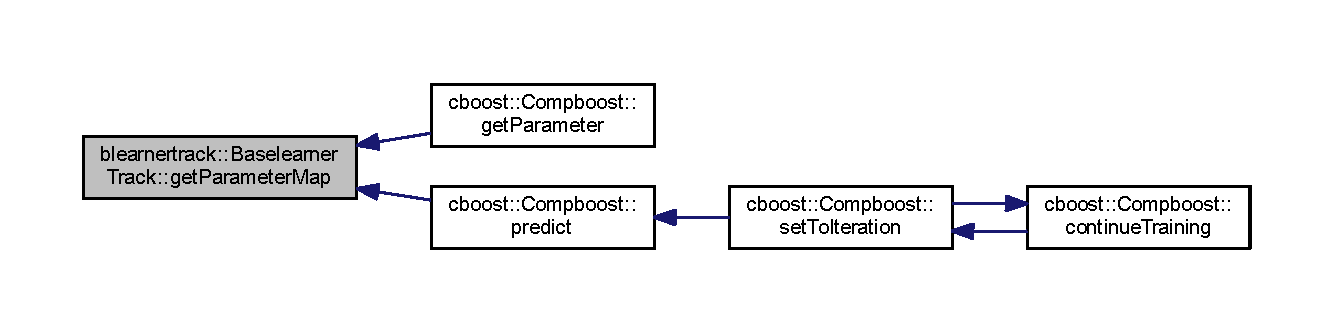
\includegraphics[width=350pt]{classblearnertrack_1_1_baselearner_track_a0ba8e3943b998b58375b892f40f12c73_icgraph}
\end{center}
\end{figure}
\mbox{\Hypertarget{classblearnertrack_1_1_baselearner_track_a4b6d2d8b585148c71ed5b6055c9ab08c}\label{classblearnertrack_1_1_baselearner_track_a4b6d2d8b585148c71ed5b6055c9ab08c}} 
\index{blearnertrack\+::\+Baselearner\+Track@{blearnertrack\+::\+Baselearner\+Track}!get\+Parameter\+Matrix@{get\+Parameter\+Matrix}}
\index{get\+Parameter\+Matrix@{get\+Parameter\+Matrix}!blearnertrack\+::\+Baselearner\+Track@{blearnertrack\+::\+Baselearner\+Track}}
\subsubsection{\texorpdfstring{get\+Parameter\+Matrix()}{getParameterMatrix()}}
{\footnotesize\ttfamily std\+::pair$<$ std\+::vector$<$ std\+::string $>$, arma\+::mat $>$ blearnertrack\+::\+Baselearner\+Track\+::get\+Parameter\+Matrix (\begin{DoxyParamCaption}{ }\end{DoxyParamCaption}) const}

Here is the caller graph for this function\+:\nopagebreak
\begin{figure}[H]
\begin{center}
\leavevmode
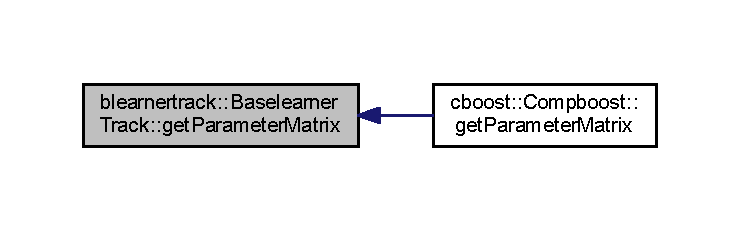
\includegraphics[width=350pt]{classblearnertrack_1_1_baselearner_track_a4b6d2d8b585148c71ed5b6055c9ab08c_icgraph}
\end{center}
\end{figure}
\mbox{\Hypertarget{classblearnertrack_1_1_baselearner_track_abc5f42093449e665b5b0dfeee8570953}\label{classblearnertrack_1_1_baselearner_track_abc5f42093449e665b5b0dfeee8570953}} 
\index{blearnertrack\+::\+Baselearner\+Track@{blearnertrack\+::\+Baselearner\+Track}!insert\+Baselearner@{insert\+Baselearner}}
\index{insert\+Baselearner@{insert\+Baselearner}!blearnertrack\+::\+Baselearner\+Track@{blearnertrack\+::\+Baselearner\+Track}}
\subsubsection{\texorpdfstring{insert\+Baselearner()}{insertBaselearner()}}
{\footnotesize\ttfamily void blearnertrack\+::\+Baselearner\+Track\+::insert\+Baselearner (\begin{DoxyParamCaption}\item[{\mbox{\hyperlink{classblearner_1_1_baselearner}{blearner\+::\+Baselearner}} $\ast$}]{blearner }\end{DoxyParamCaption})}

Here is the caller graph for this function\+:
\nopagebreak
\begin{figure}[H]
\begin{center}
\leavevmode
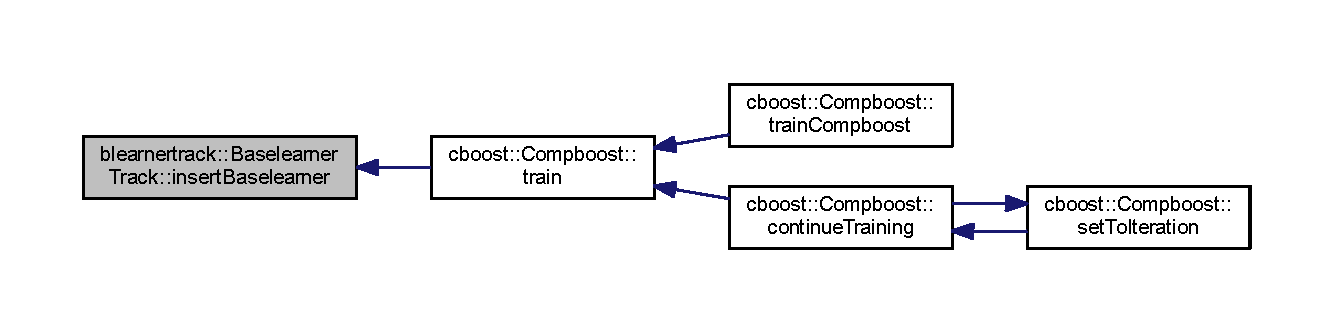
\includegraphics[width=350pt]{classblearnertrack_1_1_baselearner_track_abc5f42093449e665b5b0dfeee8570953_icgraph}
\end{center}
\end{figure}
\mbox{\Hypertarget{classblearnertrack_1_1_baselearner_track_a06f0ac986a158eecddce64e6c7af0750}\label{classblearnertrack_1_1_baselearner_track_a06f0ac986a158eecddce64e6c7af0750}} 
\index{blearnertrack\+::\+Baselearner\+Track@{blearnertrack\+::\+Baselearner\+Track}!set\+To\+Iteration@{set\+To\+Iteration}}
\index{set\+To\+Iteration@{set\+To\+Iteration}!blearnertrack\+::\+Baselearner\+Track@{blearnertrack\+::\+Baselearner\+Track}}
\subsubsection{\texorpdfstring{set\+To\+Iteration()}{setToIteration()}}
{\footnotesize\ttfamily void blearnertrack\+::\+Baselearner\+Track\+::set\+To\+Iteration (\begin{DoxyParamCaption}\item[{const unsigned int \&}]{k }\end{DoxyParamCaption})}

Here is the call graph for this function\+:
\nopagebreak
\begin{figure}[H]
\begin{center}
\leavevmode
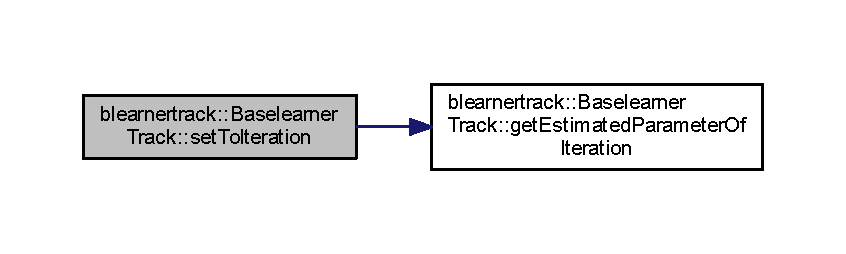
\includegraphics[width=350pt]{classblearnertrack_1_1_baselearner_track_a06f0ac986a158eecddce64e6c7af0750_cgraph}
\end{center}
\end{figure}
Here is the caller graph for this function\+:
\nopagebreak
\begin{figure}[H]
\begin{center}
\leavevmode
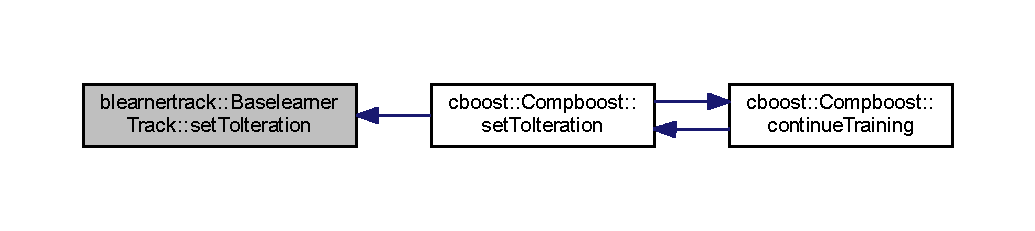
\includegraphics[width=350pt]{classblearnertrack_1_1_baselearner_track_a06f0ac986a158eecddce64e6c7af0750_icgraph}
\end{center}
\end{figure}


\subsection{Member Data Documentation}
\mbox{\Hypertarget{classblearnertrack_1_1_baselearner_track_ad37a3a99c04778146256e50c44f2a292}\label{classblearnertrack_1_1_baselearner_track_ad37a3a99c04778146256e50c44f2a292}} 
\index{blearnertrack\+::\+Baselearner\+Track@{blearnertrack\+::\+Baselearner\+Track}!blearner\+\_\+vector@{blearner\+\_\+vector}}
\index{blearner\+\_\+vector@{blearner\+\_\+vector}!blearnertrack\+::\+Baselearner\+Track@{blearnertrack\+::\+Baselearner\+Track}}
\subsubsection{\texorpdfstring{blearner\+\_\+vector}{blearner\_vector}}
{\footnotesize\ttfamily std\+::vector$<$\mbox{\hyperlink{classblearner_1_1_baselearner}{blearner\+::\+Baselearner}}$\ast$$>$ blearnertrack\+::\+Baselearner\+Track\+::blearner\+\_\+vector\hspace{0.3cm}{\ttfamily [private]}}

\mbox{\Hypertarget{classblearnertrack_1_1_baselearner_track_a62d743fe6171c52410e2f5da3dc58ffb}\label{classblearnertrack_1_1_baselearner_track_a62d743fe6171c52410e2f5da3dc58ffb}} 
\index{blearnertrack\+::\+Baselearner\+Track@{blearnertrack\+::\+Baselearner\+Track}!learning\+\_\+rate@{learning\+\_\+rate}}
\index{learning\+\_\+rate@{learning\+\_\+rate}!blearnertrack\+::\+Baselearner\+Track@{blearnertrack\+::\+Baselearner\+Track}}
\subsubsection{\texorpdfstring{learning\+\_\+rate}{learning\_rate}}
{\footnotesize\ttfamily double blearnertrack\+::\+Baselearner\+Track\+::learning\+\_\+rate\hspace{0.3cm}{\ttfamily [private]}}

\mbox{\Hypertarget{classblearnertrack_1_1_baselearner_track_a3725470c87e28ea32d4b184f1e6aad39}\label{classblearnertrack_1_1_baselearner_track_a3725470c87e28ea32d4b184f1e6aad39}} 
\index{blearnertrack\+::\+Baselearner\+Track@{blearnertrack\+::\+Baselearner\+Track}!my\+\_\+parameter\+\_\+map@{my\+\_\+parameter\+\_\+map}}
\index{my\+\_\+parameter\+\_\+map@{my\+\_\+parameter\+\_\+map}!blearnertrack\+::\+Baselearner\+Track@{blearnertrack\+::\+Baselearner\+Track}}
\subsubsection{\texorpdfstring{my\+\_\+parameter\+\_\+map}{my\_parameter\_map}}
{\footnotesize\ttfamily std\+::map$<$std\+::string, arma\+::mat$>$ blearnertrack\+::\+Baselearner\+Track\+::my\+\_\+parameter\+\_\+map\hspace{0.3cm}{\ttfamily [private]}}



The documentation for this class was generated from the following files\+:\begin{DoxyCompactItemize}
\item 
C\+:/\+Users/schal/\+One\+Drive/github\+\_\+repos/compboost/src/\mbox{\hyperlink{baselearner__track_8h}{baselearner\+\_\+track.\+h}}\item 
C\+:/\+Users/schal/\+One\+Drive/github\+\_\+repos/compboost/src/\mbox{\hyperlink{baselearner__track_8cpp}{baselearner\+\_\+track.\+cpp}}\end{DoxyCompactItemize}

\hypertarget{classloss_1_1_bernoulli_loss}{}\section{loss\+:\+:Bernoulli\+Loss Class Reference}
\label{classloss_1_1_bernoulli_loss}\index{loss\+::\+Bernoulli\+Loss@{loss\+::\+Bernoulli\+Loss}}


0-\/1 \mbox{\hyperlink{classloss_1_1_loss}{Loss}} for binary classification derifed of the bernoulli distribution  




{\ttfamily \#include $<$loss.\+h$>$}



Inheritance diagram for loss\+:\+:Bernoulli\+Loss\+:\nopagebreak
\begin{figure}[H]
\begin{center}
\leavevmode
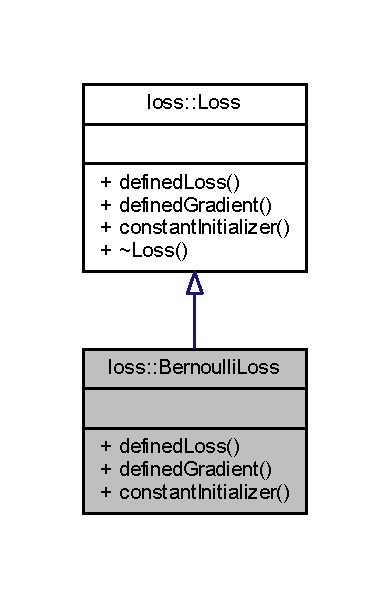
\includegraphics[width=187pt]{classloss_1_1_bernoulli_loss__inherit__graph}
\end{center}
\end{figure}


Collaboration diagram for loss\+:\+:Bernoulli\+Loss\+:\nopagebreak
\begin{figure}[H]
\begin{center}
\leavevmode
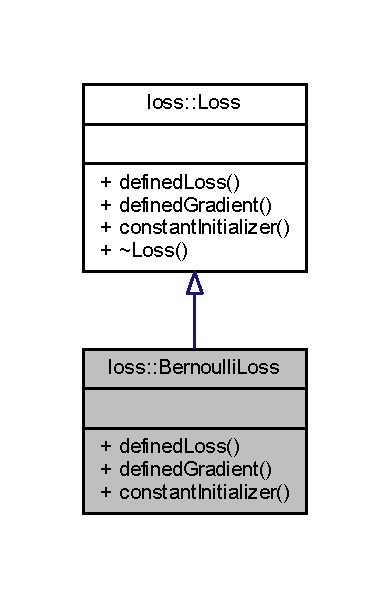
\includegraphics[width=187pt]{classloss_1_1_bernoulli_loss__coll__graph}
\end{center}
\end{figure}
\subsection*{Public Member Functions}
\begin{DoxyCompactItemize}
\item 
\mbox{\hyperlink{classloss_1_1_bernoulli_loss_a34a87f0a059b9d7346816a20818a8ac1}{Bernoulli\+Loss}} ()
\begin{DoxyCompactList}\small\item\em Default Constructor. \end{DoxyCompactList}\item 
\mbox{\hyperlink{classloss_1_1_bernoulli_loss_afc952349e055f2cd8058015960619cc8}{Bernoulli\+Loss}} (const double \&)
\begin{DoxyCompactList}\small\item\em Constructor to initialize custom offset. \end{DoxyCompactList}\item 
arma\+::vec \mbox{\hyperlink{classloss_1_1_bernoulli_loss_a1e347cacc5a5925874f579834f421236}{defined\+Loss}} (const arma\+::vec \&, const arma\+::vec \&) const
\begin{DoxyCompactList}\small\item\em Specific loss function. \end{DoxyCompactList}\item 
arma\+::vec \mbox{\hyperlink{classloss_1_1_bernoulli_loss_a2dc644172cea3eb84f1af5aa9217c04a}{defined\+Gradient}} (const arma\+::vec \&, const arma\+::vec \&) const
\begin{DoxyCompactList}\small\item\em Gradient of loss functions for pseudo residuals. \end{DoxyCompactList}\item 
double \mbox{\hyperlink{classloss_1_1_bernoulli_loss_a1b5e26f446f30d690abc625349f563d1}{constant\+Initializer}} (const arma\+::vec \&) const
\begin{DoxyCompactList}\small\item\em Constant initialization of the empirical risk. \end{DoxyCompactList}\end{DoxyCompactItemize}
\subsection*{Additional Inherited Members}


\subsection{Detailed Description}
0-\/1 \mbox{\hyperlink{classloss_1_1_loss}{Loss}} for binary classification derifed of the bernoulli distribution 

This loss can be used for binary classification. The coding we have chosen here acts on \[ y \in \{-1, 1\}. \]

{\bfseries \mbox{\hyperlink{classloss_1_1_loss}{Loss}} Function\+:} \[ L(y, f(x)) = \log\left\{1 + \exp\left(-yf(x)\right)\right\} \] {\bfseries Gradient\+:} \[ \frac{\delta}{\delta f(x)}\ L(y, f(x)) = - \frac{y}{1 + \exp\left(yf\right)} \] {\bfseries Initialization\+:} \[ \hat{f}^{[0]}(x) = \frac{1}{2}\log\left\{\frac{p}{1 - p}\right\} \] with \[ p = \frac{1}{n}\sum\limits_{i=1}^n\mathbb{1}_{\{y_i > 0\}} \] 

\subsection{Constructor \& Destructor Documentation}
\mbox{\Hypertarget{classloss_1_1_bernoulli_loss_a34a87f0a059b9d7346816a20818a8ac1}\label{classloss_1_1_bernoulli_loss_a34a87f0a059b9d7346816a20818a8ac1}} 
\index{loss\+::\+Bernoulli\+Loss@{loss\+::\+Bernoulli\+Loss}!Bernoulli\+Loss@{Bernoulli\+Loss}}
\index{Bernoulli\+Loss@{Bernoulli\+Loss}!loss\+::\+Bernoulli\+Loss@{loss\+::\+Bernoulli\+Loss}}
\subsubsection{\texorpdfstring{Bernoulli\+Loss()}{BernoulliLoss()}\hspace{0.1cm}{\footnotesize\ttfamily [1/2]}}
{\footnotesize\ttfamily loss\+::\+Bernoulli\+Loss\+::\+Bernoulli\+Loss (\begin{DoxyParamCaption}{ }\end{DoxyParamCaption})}



Default Constructor. 

Default constructor of {\ttfamily \mbox{\hyperlink{classloss_1_1_bernoulli_loss}{Bernoulli\+Loss}}} \mbox{\Hypertarget{classloss_1_1_bernoulli_loss_afc952349e055f2cd8058015960619cc8}\label{classloss_1_1_bernoulli_loss_afc952349e055f2cd8058015960619cc8}} 
\index{loss\+::\+Bernoulli\+Loss@{loss\+::\+Bernoulli\+Loss}!Bernoulli\+Loss@{Bernoulli\+Loss}}
\index{Bernoulli\+Loss@{Bernoulli\+Loss}!loss\+::\+Bernoulli\+Loss@{loss\+::\+Bernoulli\+Loss}}
\subsubsection{\texorpdfstring{Bernoulli\+Loss()}{BernoulliLoss()}\hspace{0.1cm}{\footnotesize\ttfamily [2/2]}}
{\footnotesize\ttfamily loss\+::\+Bernoulli\+Loss\+::\+Bernoulli\+Loss (\begin{DoxyParamCaption}\item[{const double \&}]{custom\+\_\+offset0 }\end{DoxyParamCaption})}



Constructor to initialize custom offset. 

Constructor to initialize custom offset of {\ttfamily \mbox{\hyperlink{classloss_1_1_absolute_loss}{Absolute\+Loss}}}


\begin{DoxyParams}{Parameters}
{\em custom\+\_\+offset0} & {\ttfamily double} Offset which is used instead of the pre defined initialization \\
\hline
\end{DoxyParams}


\subsection{Member Function Documentation}
\mbox{\Hypertarget{classloss_1_1_bernoulli_loss_a1b5e26f446f30d690abc625349f563d1}\label{classloss_1_1_bernoulli_loss_a1b5e26f446f30d690abc625349f563d1}} 
\index{loss\+::\+Bernoulli\+Loss@{loss\+::\+Bernoulli\+Loss}!constant\+Initializer@{constant\+Initializer}}
\index{constant\+Initializer@{constant\+Initializer}!loss\+::\+Bernoulli\+Loss@{loss\+::\+Bernoulli\+Loss}}
\subsubsection{\texorpdfstring{constant\+Initializer()}{constantInitializer()}}
{\footnotesize\ttfamily double loss\+::\+Bernoulli\+Loss\+::constant\+Initializer (\begin{DoxyParamCaption}\item[{const arma\+::vec \&}]{true\+\_\+value }\end{DoxyParamCaption}) const\hspace{0.3cm}{\ttfamily [virtual]}}



Constant initialization of the empirical risk. 

Definition of the constant risk initialization (see description of the class)


\begin{DoxyParams}{Parameters}
{\em true\+\_\+value} & {\ttfamily arma\+::vec} True value of the response\\
\hline
\end{DoxyParams}
\begin{DoxyReturn}{Returns}
{\ttfamily double} constant which minimizes the empirical risk for the given true value 
\end{DoxyReturn}


Implements \mbox{\hyperlink{classloss_1_1_loss_a65fe7dcd9370e6a549b8d1cc95fc8798}{loss\+::\+Loss}}.

\mbox{\Hypertarget{classloss_1_1_bernoulli_loss_a2dc644172cea3eb84f1af5aa9217c04a}\label{classloss_1_1_bernoulli_loss_a2dc644172cea3eb84f1af5aa9217c04a}} 
\index{loss\+::\+Bernoulli\+Loss@{loss\+::\+Bernoulli\+Loss}!defined\+Gradient@{defined\+Gradient}}
\index{defined\+Gradient@{defined\+Gradient}!loss\+::\+Bernoulli\+Loss@{loss\+::\+Bernoulli\+Loss}}
\subsubsection{\texorpdfstring{defined\+Gradient()}{definedGradient()}}
{\footnotesize\ttfamily arma\+::vec loss\+::\+Bernoulli\+Loss\+::defined\+Gradient (\begin{DoxyParamCaption}\item[{const arma\+::vec \&}]{true\+\_\+value,  }\item[{const arma\+::vec \&}]{prediction }\end{DoxyParamCaption}) const\hspace{0.3cm}{\ttfamily [virtual]}}



Gradient of loss functions for pseudo residuals. 

Definition of the gradient of the loss function (see description of the class)


\begin{DoxyParams}{Parameters}
{\em true\+\_\+value} & {\ttfamily arma\+::vec} True value of the response \\
\hline
{\em prediction} & {\ttfamily arma\+::vec} Prediction of the true value\\
\hline
\end{DoxyParams}
\begin{DoxyReturn}{Returns}
{\ttfamily arma\+::vec} vector of elementwise application of the gradient 
\end{DoxyReturn}


Implements \mbox{\hyperlink{classloss_1_1_loss_a267a4de70747ade4b2d84ce35a448979}{loss\+::\+Loss}}.

\mbox{\Hypertarget{classloss_1_1_bernoulli_loss_a1e347cacc5a5925874f579834f421236}\label{classloss_1_1_bernoulli_loss_a1e347cacc5a5925874f579834f421236}} 
\index{loss\+::\+Bernoulli\+Loss@{loss\+::\+Bernoulli\+Loss}!defined\+Loss@{defined\+Loss}}
\index{defined\+Loss@{defined\+Loss}!loss\+::\+Bernoulli\+Loss@{loss\+::\+Bernoulli\+Loss}}
\subsubsection{\texorpdfstring{defined\+Loss()}{definedLoss()}}
{\footnotesize\ttfamily arma\+::vec loss\+::\+Bernoulli\+Loss\+::defined\+Loss (\begin{DoxyParamCaption}\item[{const arma\+::vec \&}]{true\+\_\+value,  }\item[{const arma\+::vec \&}]{prediction }\end{DoxyParamCaption}) const\hspace{0.3cm}{\ttfamily [virtual]}}



Specific loss function. 

Definition of the loss function (see description of the class)


\begin{DoxyParams}{Parameters}
{\em true\+\_\+value} & {\ttfamily arma\+::vec} True value of the response \\
\hline
{\em prediction} & {\ttfamily arma\+::vec} Prediction of the true value\\
\hline
\end{DoxyParams}
\begin{DoxyReturn}{Returns}
{\ttfamily arma\+::vec} vector of elementwise application of the loss function 
\end{DoxyReturn}


Implements \mbox{\hyperlink{classloss_1_1_loss_ae9f94dd9b8311397583ba3a9cb485e94}{loss\+::\+Loss}}.



The documentation for this class was generated from the following files\+:\begin{DoxyCompactItemize}
\item 
E\+:/\+One\+Drive/github\+\_\+repos/compboost/src/\mbox{\hyperlink{loss_8h}{loss.\+h}}\item 
E\+:/\+One\+Drive/github\+\_\+repos/compboost/src/\mbox{\hyperlink{loss_8cpp}{loss.\+cpp}}\end{DoxyCompactItemize}

\hypertarget{classcboost_1_1_compboost}{}\section{cboost\+:\+:Compboost Class Reference}
\label{classcboost_1_1_compboost}\index{cboost\+::\+Compboost@{cboost\+::\+Compboost}}


{\ttfamily \#include $<$compboost.\+h$>$}



Collaboration diagram for cboost\+:\+:Compboost\+:
\nopagebreak
\begin{figure}[H]
\begin{center}
\leavevmode
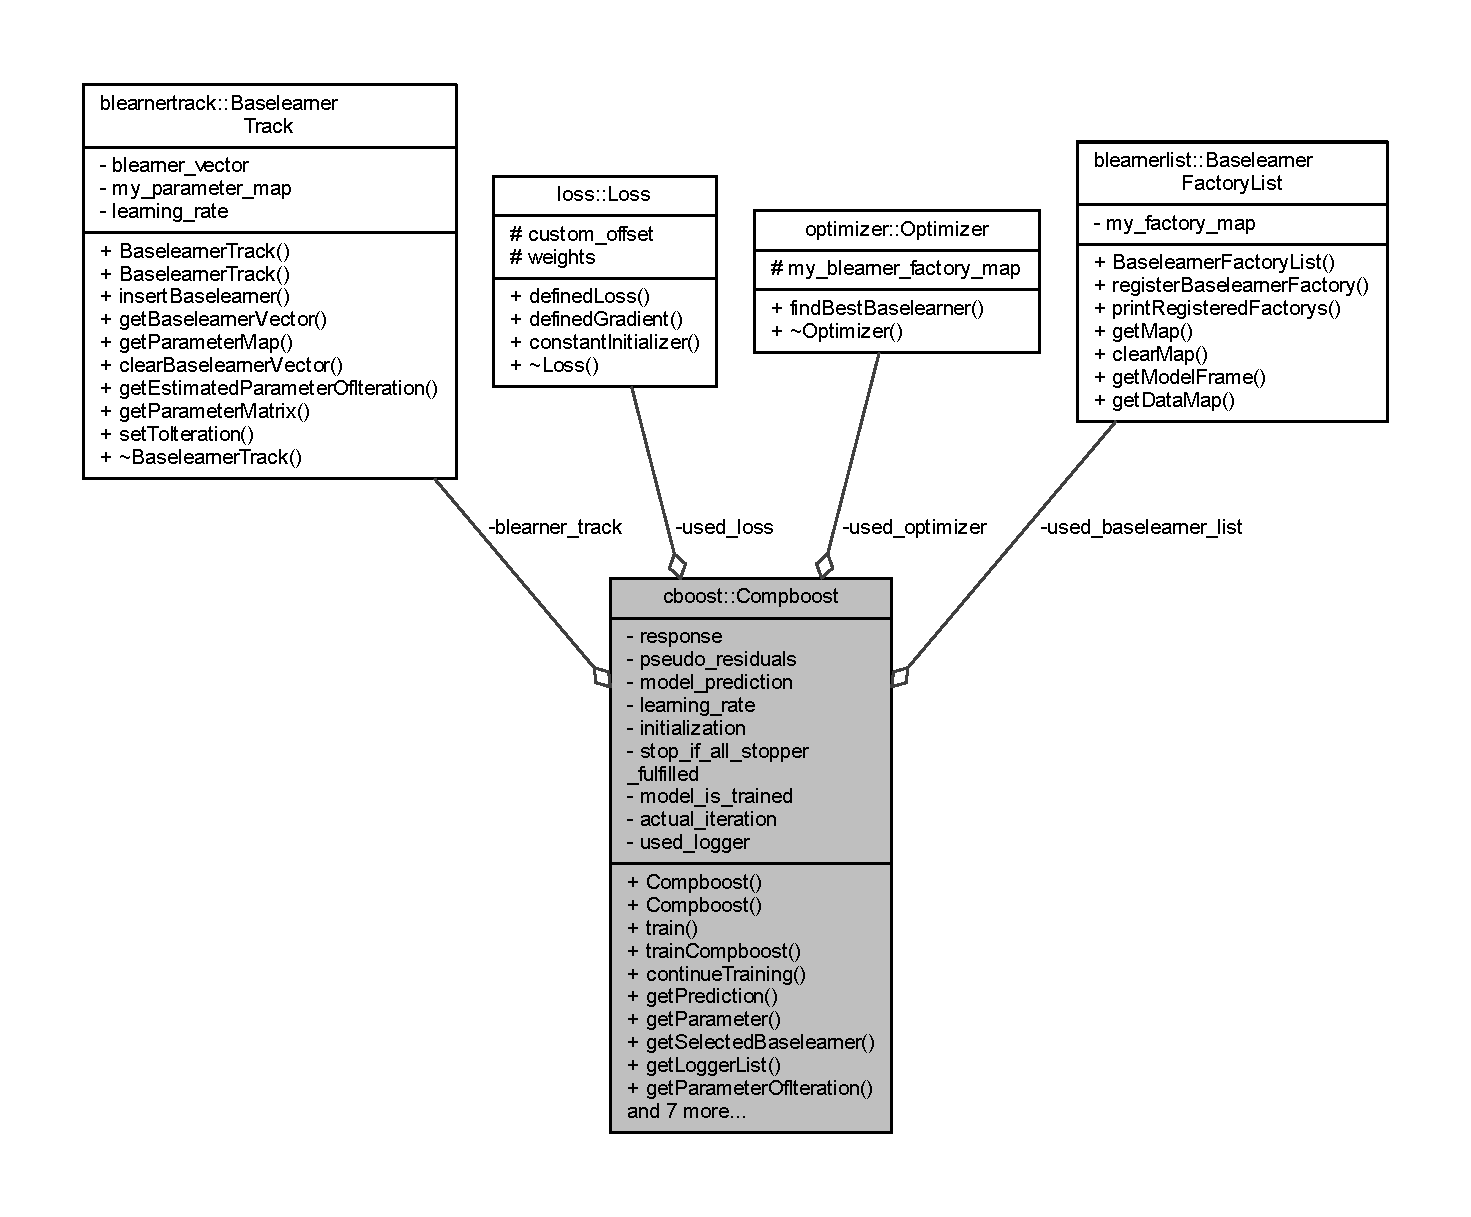
\includegraphics[width=350pt]{classcboost_1_1_compboost__coll__graph}
\end{center}
\end{figure}
\subsection*{Public Member Functions}
\begin{DoxyCompactItemize}
\item 
\mbox{\hyperlink{classcboost_1_1_compboost_a5117b7b8cf0a424e736f6833bc5c3a68}{Compboost}} ()
\item 
\mbox{\hyperlink{classcboost_1_1_compboost_a24b98d64e9aac2a7a8ec4e64a49a1f7c}{Compboost}} (const arma\+::vec \&, const double \&, const bool \&, \mbox{\hyperlink{classoptimizer_1_1_optimizer}{optimizer\+::\+Optimizer}} $\ast$, \mbox{\hyperlink{classloss_1_1_loss}{loss\+::\+Loss}} $\ast$, \mbox{\hyperlink{classloggerlist_1_1_logger_list}{loggerlist\+::\+Logger\+List}} $\ast$, \mbox{\hyperlink{classblearnerlist_1_1_baselearner_factory_list}{blearnerlist\+::\+Baselearner\+Factory\+List}})
\item 
void \mbox{\hyperlink{classcboost_1_1_compboost_aa898572eb2c83e0b95c12788a859333b}{train}} (const bool \&, const arma\+::vec \&, \mbox{\hyperlink{classloggerlist_1_1_logger_list}{loggerlist\+::\+Logger\+List}} $\ast$)
\item 
void \mbox{\hyperlink{classcboost_1_1_compboost_a52ea04dec53c68865fdc4a79461d17cb}{train\+Compboost}} (const bool \&)
\item 
void \mbox{\hyperlink{classcboost_1_1_compboost_a191aa22dbfcc3d2e878ef75c0b196d07}{continue\+Training}} (\mbox{\hyperlink{classloggerlist_1_1_logger_list}{loggerlist\+::\+Logger\+List}} $\ast$, const bool \&)
\item 
arma\+::vec \mbox{\hyperlink{classcboost_1_1_compboost_a405c6b88de5b053fefdb24742791da4e}{get\+Prediction}} () const
\item 
std\+::map$<$ std\+::string, arma\+::mat $>$ \mbox{\hyperlink{classcboost_1_1_compboost_a7b90eaa8107f91806b09ceedf8581537}{get\+Parameter}} () const
\item 
std\+::vector$<$ std\+::string $>$ \mbox{\hyperlink{classcboost_1_1_compboost_ac66d4490e6539832d4d304a86db746dc}{get\+Selected\+Baselearner}} () const
\item 
std\+::map$<$ std\+::string, \mbox{\hyperlink{classloggerlist_1_1_logger_list}{loggerlist\+::\+Logger\+List}} $\ast$ $>$ \mbox{\hyperlink{classcboost_1_1_compboost_a0376256bdfde1a50b420ad7412f4b4dd}{get\+Logger\+List}} () const
\item 
std\+::map$<$ std\+::string, arma\+::mat $>$ \mbox{\hyperlink{classcboost_1_1_compboost_a97b02aa81981e08658d896ff9798b5d0}{get\+Parameter\+Of\+Iteration}} (const unsigned int \&) const
\item 
std\+::pair$<$ std\+::vector$<$ std\+::string $>$, arma\+::mat $>$ \mbox{\hyperlink{classcboost_1_1_compboost_a1652d7fa10039beaee1998e640f1b68a}{get\+Parameter\+Matrix}} () const
\item 
arma\+::vec \mbox{\hyperlink{classcboost_1_1_compboost_a32d1066a24607ff6ef2f934002adf62b}{predict}} () const
\item 
arma\+::vec \mbox{\hyperlink{classcboost_1_1_compboost_a1779a0c89cf9da32b250c0c083631c58}{predict}} (std\+::map$<$ std\+::string, \mbox{\hyperlink{classdata_1_1_data}{data\+::\+Data}} $\ast$$>$) const
\item 
arma\+::vec \mbox{\hyperlink{classcboost_1_1_compboost_a6582a12bf1060750367219aeae395963}{prediction\+Of\+Iteration}} (std\+::map$<$ std\+::string, \mbox{\hyperlink{classdata_1_1_data}{data\+::\+Data}} $\ast$$>$, const unsigned int \&) const
\item 
void \mbox{\hyperlink{classcboost_1_1_compboost_ad1ee3b88f585f38255d827dceb4b7659}{set\+To\+Iteration}} (const unsigned int \&)
\item 
void \mbox{\hyperlink{classcboost_1_1_compboost_a7be8cb767054ece895d535c1f468233e}{summarize\+Compboost}} () const
\item 
\mbox{\hyperlink{classcboost_1_1_compboost_a3e23314cc3a1d31fc5df61e0a16c51e4}{$\sim$\+Compboost}} ()
\end{DoxyCompactItemize}
\subsection*{Private Attributes}
\begin{DoxyCompactItemize}
\item 
arma\+::vec \mbox{\hyperlink{classcboost_1_1_compboost_a01de924b977c9ba12a3f3be88e2586e4}{response}}
\item 
arma\+::vec \mbox{\hyperlink{classcboost_1_1_compboost_acb8716c9e383e15ae7d8785a591860f7}{pseudo\+\_\+residuals}}
\item 
arma\+::vec \mbox{\hyperlink{classcboost_1_1_compboost_a7f7c7fe26c16c175e7d402aca781e8da}{model\+\_\+prediction}}
\item 
double \mbox{\hyperlink{classcboost_1_1_compboost_aa6a7b77188ae60be668e87018d28835a}{learning\+\_\+rate}}
\item 
double \mbox{\hyperlink{classcboost_1_1_compboost_a2056c4035d5e0d8b0dcb4daedfadee16}{initialization}}
\item 
bool \mbox{\hyperlink{classcboost_1_1_compboost_a40c118dcaf96479cd6574138f9b2620f}{stop\+\_\+if\+\_\+all\+\_\+stopper\+\_\+fulfilled}}
\item 
bool \mbox{\hyperlink{classcboost_1_1_compboost_af1da66c1def3edd484f5d30b36e64eeb}{model\+\_\+is\+\_\+trained}} = false
\item 
unsigned int \mbox{\hyperlink{classcboost_1_1_compboost_a3db81c285c1cd238d0fb65dfc6c00439}{actual\+\_\+iteration}}
\item 
\mbox{\hyperlink{classblearnertrack_1_1_baselearner_track}{blearnertrack\+::\+Baselearner\+Track}} \mbox{\hyperlink{classcboost_1_1_compboost_af9c2787818f591941f74af0059ca7dc9}{blearner\+\_\+track}}
\item 
\mbox{\hyperlink{classoptimizer_1_1_optimizer}{optimizer\+::\+Optimizer}} $\ast$ \mbox{\hyperlink{classcboost_1_1_compboost_a6c0311a05cf6128b4c76fabbc432b807}{used\+\_\+optimizer}}
\item 
\mbox{\hyperlink{classloss_1_1_loss}{loss\+::\+Loss}} $\ast$ \mbox{\hyperlink{classcboost_1_1_compboost_a9c776faf5e9b9e99b5241f2a650d5242}{used\+\_\+loss}}
\item 
\mbox{\hyperlink{classblearnerlist_1_1_baselearner_factory_list}{blearnerlist\+::\+Baselearner\+Factory\+List}} \mbox{\hyperlink{classcboost_1_1_compboost_ac4c690473dc39e10e84ae9d9219b1fa1}{used\+\_\+baselearner\+\_\+list}}
\item 
std\+::map$<$ std\+::string, \mbox{\hyperlink{classloggerlist_1_1_logger_list}{loggerlist\+::\+Logger\+List}} $\ast$ $>$ \mbox{\hyperlink{classcboost_1_1_compboost_a05590928bf741eecb135f32da339ceaa}{used\+\_\+logger}}
\end{DoxyCompactItemize}


\subsection{Constructor \& Destructor Documentation}
\mbox{\Hypertarget{classcboost_1_1_compboost_a5117b7b8cf0a424e736f6833bc5c3a68}\label{classcboost_1_1_compboost_a5117b7b8cf0a424e736f6833bc5c3a68}} 
\index{cboost\+::\+Compboost@{cboost\+::\+Compboost}!Compboost@{Compboost}}
\index{Compboost@{Compboost}!cboost\+::\+Compboost@{cboost\+::\+Compboost}}
\subsubsection{\texorpdfstring{Compboost()}{Compboost()}\hspace{0.1cm}{\footnotesize\ttfamily [1/2]}}
{\footnotesize\ttfamily cboost\+::\+Compboost\+::\+Compboost (\begin{DoxyParamCaption}{ }\end{DoxyParamCaption})}

\mbox{\Hypertarget{classcboost_1_1_compboost_a24b98d64e9aac2a7a8ec4e64a49a1f7c}\label{classcboost_1_1_compboost_a24b98d64e9aac2a7a8ec4e64a49a1f7c}} 
\index{cboost\+::\+Compboost@{cboost\+::\+Compboost}!Compboost@{Compboost}}
\index{Compboost@{Compboost}!cboost\+::\+Compboost@{cboost\+::\+Compboost}}
\subsubsection{\texorpdfstring{Compboost()}{Compboost()}\hspace{0.1cm}{\footnotesize\ttfamily [2/2]}}
{\footnotesize\ttfamily cboost\+::\+Compboost\+::\+Compboost (\begin{DoxyParamCaption}\item[{const arma\+::vec \&}]{response,  }\item[{const double \&}]{learning\+\_\+rate,  }\item[{const bool \&}]{stop\+\_\+if\+\_\+all\+\_\+stopper\+\_\+fulfilled,  }\item[{\mbox{\hyperlink{classoptimizer_1_1_optimizer}{optimizer\+::\+Optimizer}} $\ast$}]{used\+\_\+optimizer,  }\item[{\mbox{\hyperlink{classloss_1_1_loss}{loss\+::\+Loss}} $\ast$}]{used\+\_\+loss,  }\item[{\mbox{\hyperlink{classloggerlist_1_1_logger_list}{loggerlist\+::\+Logger\+List}} $\ast$}]{used\+\_\+logger0,  }\item[{\mbox{\hyperlink{classblearnerlist_1_1_baselearner_factory_list}{blearnerlist\+::\+Baselearner\+Factory\+List}}}]{used\+\_\+baselearner\+\_\+list }\end{DoxyParamCaption})}

\mbox{\Hypertarget{classcboost_1_1_compboost_a3e23314cc3a1d31fc5df61e0a16c51e4}\label{classcboost_1_1_compboost_a3e23314cc3a1d31fc5df61e0a16c51e4}} 
\index{cboost\+::\+Compboost@{cboost\+::\+Compboost}!````~Compboost@{$\sim$\+Compboost}}
\index{````~Compboost@{$\sim$\+Compboost}!cboost\+::\+Compboost@{cboost\+::\+Compboost}}
\subsubsection{\texorpdfstring{$\sim$\+Compboost()}{~Compboost()}}
{\footnotesize\ttfamily cboost\+::\+Compboost\+::$\sim$\+Compboost (\begin{DoxyParamCaption}{ }\end{DoxyParamCaption})}



\subsection{Member Function Documentation}
\mbox{\Hypertarget{classcboost_1_1_compboost_a191aa22dbfcc3d2e878ef75c0b196d07}\label{classcboost_1_1_compboost_a191aa22dbfcc3d2e878ef75c0b196d07}} 
\index{cboost\+::\+Compboost@{cboost\+::\+Compboost}!continue\+Training@{continue\+Training}}
\index{continue\+Training@{continue\+Training}!cboost\+::\+Compboost@{cboost\+::\+Compboost}}
\subsubsection{\texorpdfstring{continue\+Training()}{continueTraining()}}
{\footnotesize\ttfamily void cboost\+::\+Compboost\+::continue\+Training (\begin{DoxyParamCaption}\item[{\mbox{\hyperlink{classloggerlist_1_1_logger_list}{loggerlist\+::\+Logger\+List}} $\ast$}]{logger,  }\item[{const bool \&}]{trace }\end{DoxyParamCaption})}

Here is the call graph for this function\+:\nopagebreak
\begin{figure}[H]
\begin{center}
\leavevmode
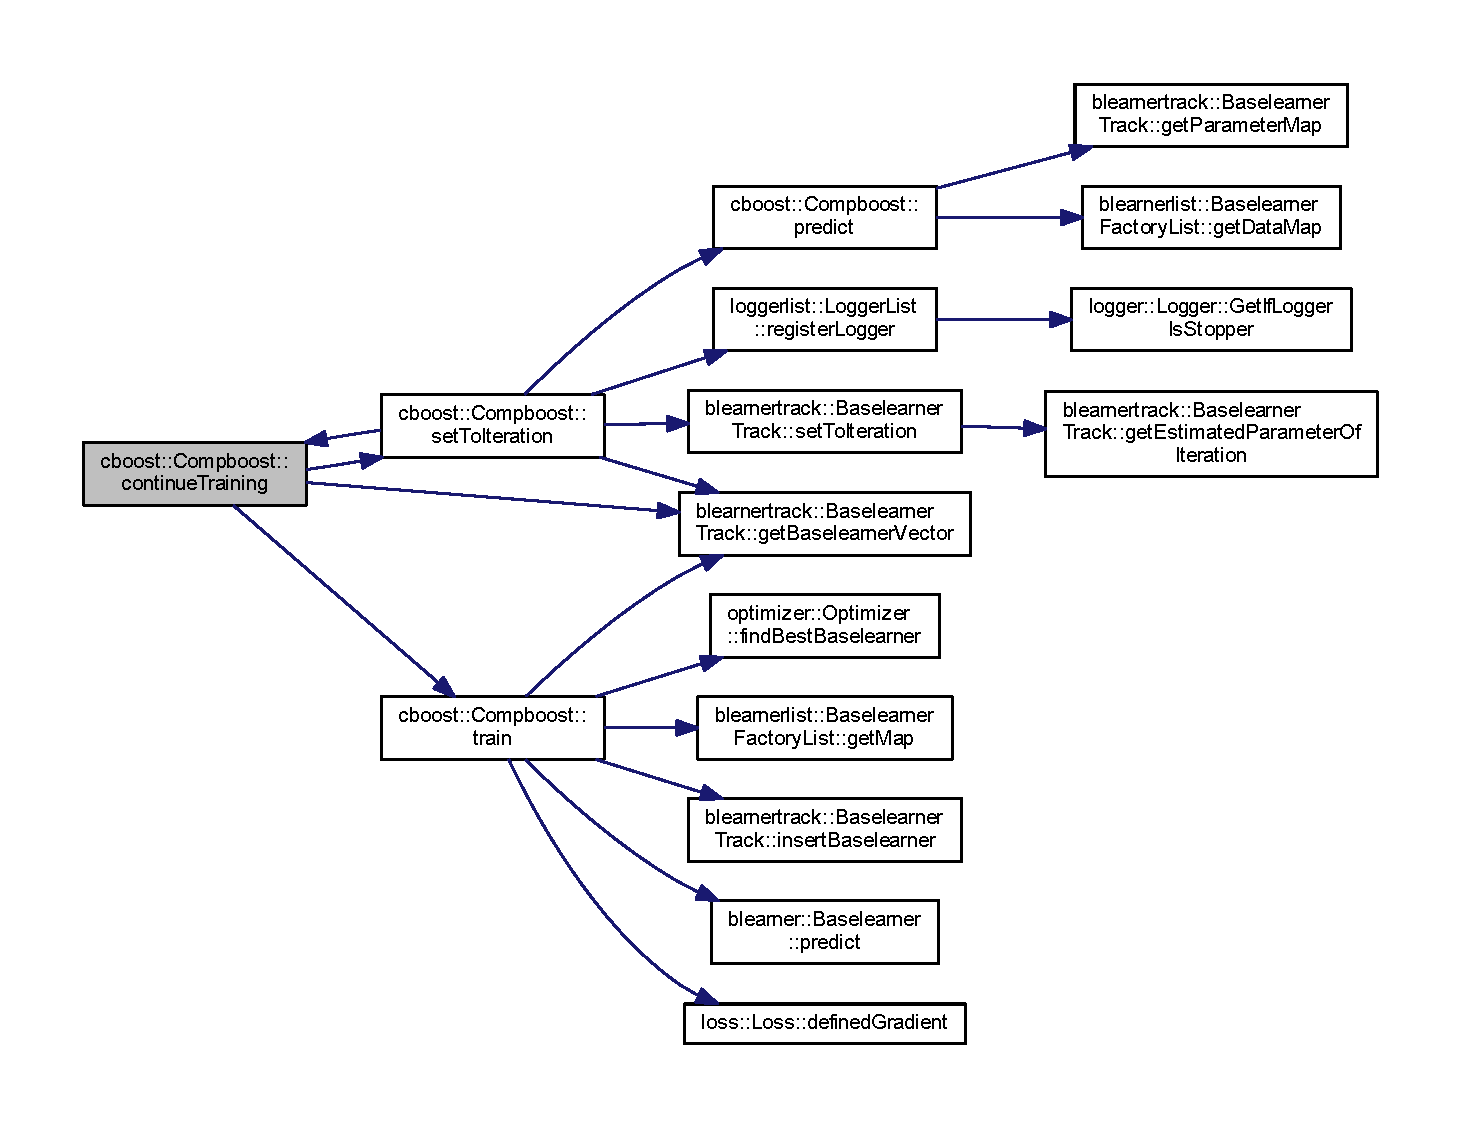
\includegraphics[width=350pt]{classcboost_1_1_compboost_a191aa22dbfcc3d2e878ef75c0b196d07_cgraph}
\end{center}
\end{figure}
Here is the caller graph for this function\+:\nopagebreak
\begin{figure}[H]
\begin{center}
\leavevmode
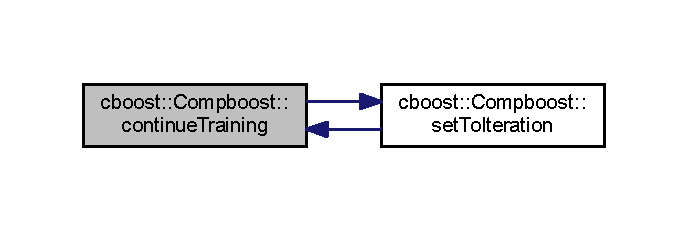
\includegraphics[width=330pt]{classcboost_1_1_compboost_a191aa22dbfcc3d2e878ef75c0b196d07_icgraph}
\end{center}
\end{figure}
\mbox{\Hypertarget{classcboost_1_1_compboost_a0376256bdfde1a50b420ad7412f4b4dd}\label{classcboost_1_1_compboost_a0376256bdfde1a50b420ad7412f4b4dd}} 
\index{cboost\+::\+Compboost@{cboost\+::\+Compboost}!get\+Logger\+List@{get\+Logger\+List}}
\index{get\+Logger\+List@{get\+Logger\+List}!cboost\+::\+Compboost@{cboost\+::\+Compboost}}
\subsubsection{\texorpdfstring{get\+Logger\+List()}{getLoggerList()}}
{\footnotesize\ttfamily std\+::map$<$ std\+::string, \mbox{\hyperlink{classloggerlist_1_1_logger_list}{loggerlist\+::\+Logger\+List}} $\ast$ $>$ cboost\+::\+Compboost\+::get\+Logger\+List (\begin{DoxyParamCaption}{ }\end{DoxyParamCaption}) const}

\mbox{\Hypertarget{classcboost_1_1_compboost_a7b90eaa8107f91806b09ceedf8581537}\label{classcboost_1_1_compboost_a7b90eaa8107f91806b09ceedf8581537}} 
\index{cboost\+::\+Compboost@{cboost\+::\+Compboost}!get\+Parameter@{get\+Parameter}}
\index{get\+Parameter@{get\+Parameter}!cboost\+::\+Compboost@{cboost\+::\+Compboost}}
\subsubsection{\texorpdfstring{get\+Parameter()}{getParameter()}}
{\footnotesize\ttfamily std\+::map$<$ std\+::string, arma\+::mat $>$ cboost\+::\+Compboost\+::get\+Parameter (\begin{DoxyParamCaption}{ }\end{DoxyParamCaption}) const}

Here is the call graph for this function\+:\nopagebreak
\begin{figure}[H]
\begin{center}
\leavevmode
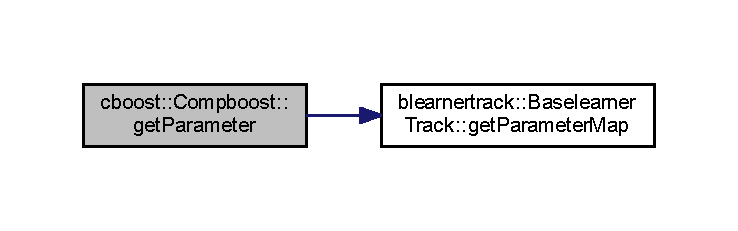
\includegraphics[width=350pt]{classcboost_1_1_compboost_a7b90eaa8107f91806b09ceedf8581537_cgraph}
\end{center}
\end{figure}
\mbox{\Hypertarget{classcboost_1_1_compboost_a1652d7fa10039beaee1998e640f1b68a}\label{classcboost_1_1_compboost_a1652d7fa10039beaee1998e640f1b68a}} 
\index{cboost\+::\+Compboost@{cboost\+::\+Compboost}!get\+Parameter\+Matrix@{get\+Parameter\+Matrix}}
\index{get\+Parameter\+Matrix@{get\+Parameter\+Matrix}!cboost\+::\+Compboost@{cboost\+::\+Compboost}}
\subsubsection{\texorpdfstring{get\+Parameter\+Matrix()}{getParameterMatrix()}}
{\footnotesize\ttfamily std\+::pair$<$ std\+::vector$<$ std\+::string $>$, arma\+::mat $>$ cboost\+::\+Compboost\+::get\+Parameter\+Matrix (\begin{DoxyParamCaption}{ }\end{DoxyParamCaption}) const}

Here is the call graph for this function\+:\nopagebreak
\begin{figure}[H]
\begin{center}
\leavevmode
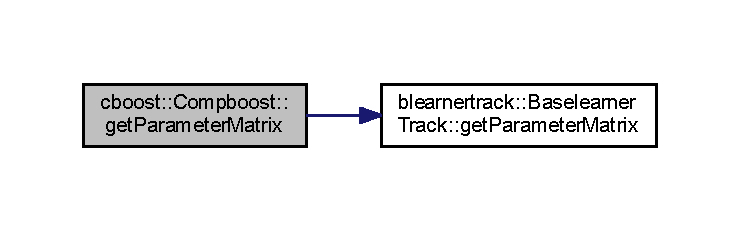
\includegraphics[width=350pt]{classcboost_1_1_compboost_a1652d7fa10039beaee1998e640f1b68a_cgraph}
\end{center}
\end{figure}
\mbox{\Hypertarget{classcboost_1_1_compboost_a97b02aa81981e08658d896ff9798b5d0}\label{classcboost_1_1_compboost_a97b02aa81981e08658d896ff9798b5d0}} 
\index{cboost\+::\+Compboost@{cboost\+::\+Compboost}!get\+Parameter\+Of\+Iteration@{get\+Parameter\+Of\+Iteration}}
\index{get\+Parameter\+Of\+Iteration@{get\+Parameter\+Of\+Iteration}!cboost\+::\+Compboost@{cboost\+::\+Compboost}}
\subsubsection{\texorpdfstring{get\+Parameter\+Of\+Iteration()}{getParameterOfIteration()}}
{\footnotesize\ttfamily std\+::map$<$ std\+::string, arma\+::mat $>$ cboost\+::\+Compboost\+::get\+Parameter\+Of\+Iteration (\begin{DoxyParamCaption}\item[{const unsigned int \&}]{k }\end{DoxyParamCaption}) const}

Here is the call graph for this function\+:\nopagebreak
\begin{figure}[H]
\begin{center}
\leavevmode
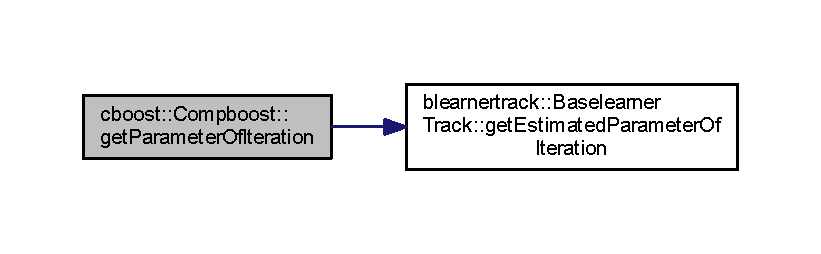
\includegraphics[width=350pt]{classcboost_1_1_compboost_a97b02aa81981e08658d896ff9798b5d0_cgraph}
\end{center}
\end{figure}
\mbox{\Hypertarget{classcboost_1_1_compboost_a405c6b88de5b053fefdb24742791da4e}\label{classcboost_1_1_compboost_a405c6b88de5b053fefdb24742791da4e}} 
\index{cboost\+::\+Compboost@{cboost\+::\+Compboost}!get\+Prediction@{get\+Prediction}}
\index{get\+Prediction@{get\+Prediction}!cboost\+::\+Compboost@{cboost\+::\+Compboost}}
\subsubsection{\texorpdfstring{get\+Prediction()}{getPrediction()}}
{\footnotesize\ttfamily arma\+::vec cboost\+::\+Compboost\+::get\+Prediction (\begin{DoxyParamCaption}{ }\end{DoxyParamCaption}) const}

\mbox{\Hypertarget{classcboost_1_1_compboost_ac66d4490e6539832d4d304a86db746dc}\label{classcboost_1_1_compboost_ac66d4490e6539832d4d304a86db746dc}} 
\index{cboost\+::\+Compboost@{cboost\+::\+Compboost}!get\+Selected\+Baselearner@{get\+Selected\+Baselearner}}
\index{get\+Selected\+Baselearner@{get\+Selected\+Baselearner}!cboost\+::\+Compboost@{cboost\+::\+Compboost}}
\subsubsection{\texorpdfstring{get\+Selected\+Baselearner()}{getSelectedBaselearner()}}
{\footnotesize\ttfamily std\+::vector$<$ std\+::string $>$ cboost\+::\+Compboost\+::get\+Selected\+Baselearner (\begin{DoxyParamCaption}{ }\end{DoxyParamCaption}) const}

Here is the call graph for this function\+:\nopagebreak
\begin{figure}[H]
\begin{center}
\leavevmode
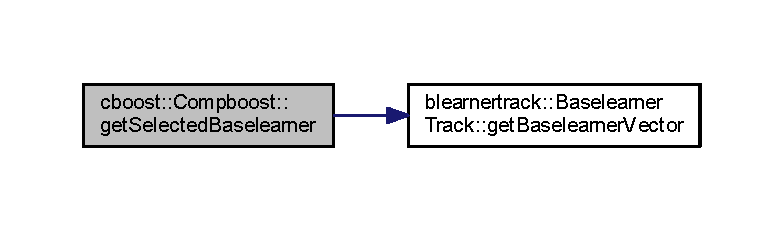
\includegraphics[width=350pt]{classcboost_1_1_compboost_ac66d4490e6539832d4d304a86db746dc_cgraph}
\end{center}
\end{figure}
\mbox{\Hypertarget{classcboost_1_1_compboost_a32d1066a24607ff6ef2f934002adf62b}\label{classcboost_1_1_compboost_a32d1066a24607ff6ef2f934002adf62b}} 
\index{cboost\+::\+Compboost@{cboost\+::\+Compboost}!predict@{predict}}
\index{predict@{predict}!cboost\+::\+Compboost@{cboost\+::\+Compboost}}
\subsubsection{\texorpdfstring{predict()}{predict()}\hspace{0.1cm}{\footnotesize\ttfamily [1/2]}}
{\footnotesize\ttfamily arma\+::vec cboost\+::\+Compboost\+::predict (\begin{DoxyParamCaption}{ }\end{DoxyParamCaption}) const}

Here is the call graph for this function\+:\nopagebreak
\begin{figure}[H]
\begin{center}
\leavevmode
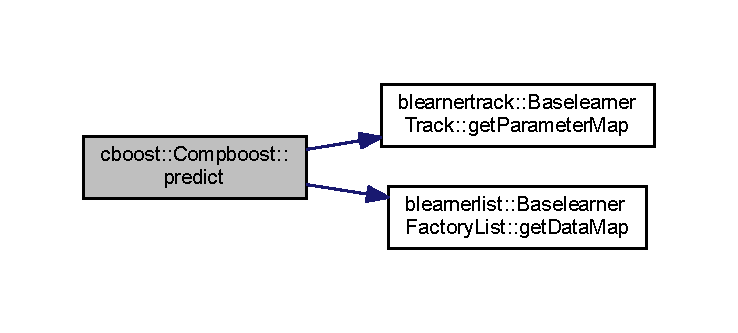
\includegraphics[width=350pt]{classcboost_1_1_compboost_a32d1066a24607ff6ef2f934002adf62b_cgraph}
\end{center}
\end{figure}
Here is the caller graph for this function\+:\nopagebreak
\begin{figure}[H]
\begin{center}
\leavevmode
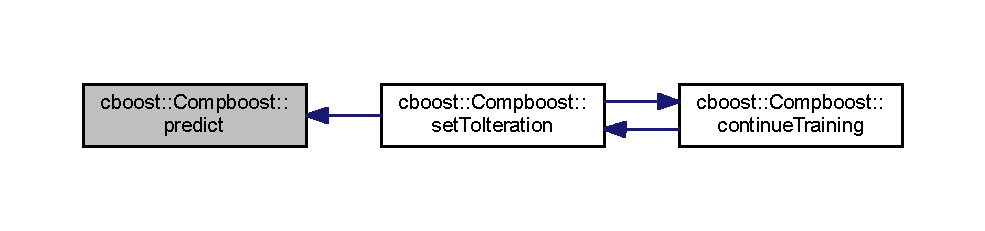
\includegraphics[width=350pt]{classcboost_1_1_compboost_a32d1066a24607ff6ef2f934002adf62b_icgraph}
\end{center}
\end{figure}
\mbox{\Hypertarget{classcboost_1_1_compboost_a1779a0c89cf9da32b250c0c083631c58}\label{classcboost_1_1_compboost_a1779a0c89cf9da32b250c0c083631c58}} 
\index{cboost\+::\+Compboost@{cboost\+::\+Compboost}!predict@{predict}}
\index{predict@{predict}!cboost\+::\+Compboost@{cboost\+::\+Compboost}}
\subsubsection{\texorpdfstring{predict()}{predict()}\hspace{0.1cm}{\footnotesize\ttfamily [2/2]}}
{\footnotesize\ttfamily arma\+::vec cboost\+::\+Compboost\+::predict (\begin{DoxyParamCaption}\item[{std\+::map$<$ std\+::string, \mbox{\hyperlink{classdata_1_1_data}{data\+::\+Data}} $\ast$$>$}]{data\+\_\+map }\end{DoxyParamCaption}) const}

Here is the call graph for this function\+:\nopagebreak
\begin{figure}[H]
\begin{center}
\leavevmode
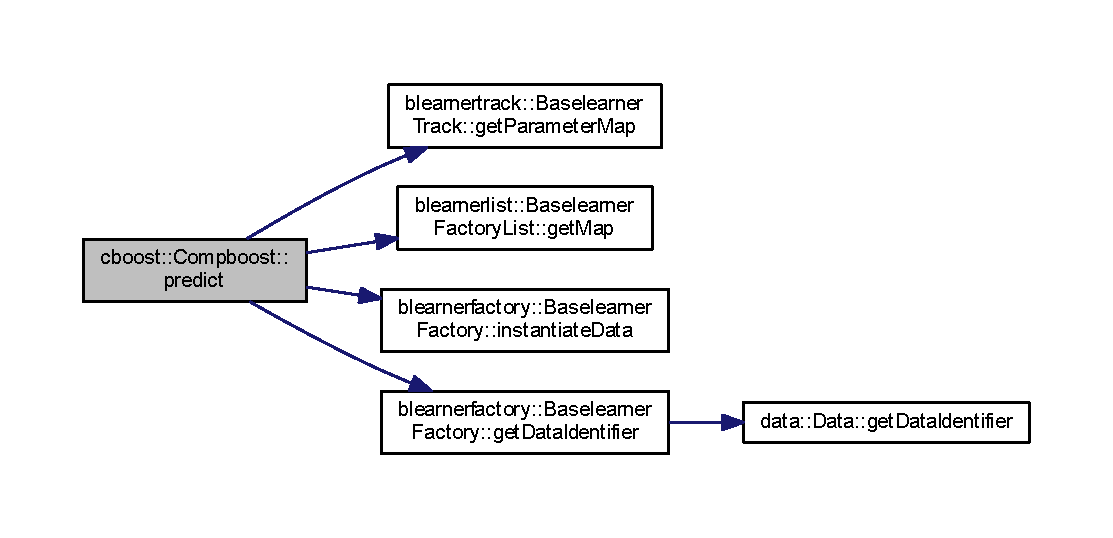
\includegraphics[width=350pt]{classcboost_1_1_compboost_a1779a0c89cf9da32b250c0c083631c58_cgraph}
\end{center}
\end{figure}
\mbox{\Hypertarget{classcboost_1_1_compboost_a6582a12bf1060750367219aeae395963}\label{classcboost_1_1_compboost_a6582a12bf1060750367219aeae395963}} 
\index{cboost\+::\+Compboost@{cboost\+::\+Compboost}!prediction\+Of\+Iteration@{prediction\+Of\+Iteration}}
\index{prediction\+Of\+Iteration@{prediction\+Of\+Iteration}!cboost\+::\+Compboost@{cboost\+::\+Compboost}}
\subsubsection{\texorpdfstring{prediction\+Of\+Iteration()}{predictionOfIteration()}}
{\footnotesize\ttfamily arma\+::vec cboost\+::\+Compboost\+::prediction\+Of\+Iteration (\begin{DoxyParamCaption}\item[{std\+::map$<$ std\+::string, \mbox{\hyperlink{classdata_1_1_data}{data\+::\+Data}} $\ast$$>$}]{data\+\_\+map,  }\item[{const unsigned int \&}]{k }\end{DoxyParamCaption}) const}

Here is the call graph for this function\+:\nopagebreak
\begin{figure}[H]
\begin{center}
\leavevmode
\includegraphics[width=350pt]{classcboost_1_1_compboost_a6582a12bf1060750367219aeae395963_cgraph}
\end{center}
\end{figure}
\mbox{\Hypertarget{classcboost_1_1_compboost_ad1ee3b88f585f38255d827dceb4b7659}\label{classcboost_1_1_compboost_ad1ee3b88f585f38255d827dceb4b7659}} 
\index{cboost\+::\+Compboost@{cboost\+::\+Compboost}!set\+To\+Iteration@{set\+To\+Iteration}}
\index{set\+To\+Iteration@{set\+To\+Iteration}!cboost\+::\+Compboost@{cboost\+::\+Compboost}}
\subsubsection{\texorpdfstring{set\+To\+Iteration()}{setToIteration()}}
{\footnotesize\ttfamily void cboost\+::\+Compboost\+::set\+To\+Iteration (\begin{DoxyParamCaption}\item[{const unsigned int \&}]{k }\end{DoxyParamCaption})}

Here is the call graph for this function\+:\nopagebreak
\begin{figure}[H]
\begin{center}
\leavevmode
\includegraphics[width=350pt]{classcboost_1_1_compboost_ad1ee3b88f585f38255d827dceb4b7659_cgraph}
\end{center}
\end{figure}
Here is the caller graph for this function\+:\nopagebreak
\begin{figure}[H]
\begin{center}
\leavevmode
\includegraphics[width=330pt]{classcboost_1_1_compboost_ad1ee3b88f585f38255d827dceb4b7659_icgraph}
\end{center}
\end{figure}
\mbox{\Hypertarget{classcboost_1_1_compboost_a7be8cb767054ece895d535c1f468233e}\label{classcboost_1_1_compboost_a7be8cb767054ece895d535c1f468233e}} 
\index{cboost\+::\+Compboost@{cboost\+::\+Compboost}!summarize\+Compboost@{summarize\+Compboost}}
\index{summarize\+Compboost@{summarize\+Compboost}!cboost\+::\+Compboost@{cboost\+::\+Compboost}}
\subsubsection{\texorpdfstring{summarize\+Compboost()}{summarizeCompboost()}}
{\footnotesize\ttfamily void cboost\+::\+Compboost\+::summarize\+Compboost (\begin{DoxyParamCaption}{ }\end{DoxyParamCaption}) const}

Here is the call graph for this function\+:\nopagebreak
\begin{figure}[H]
\begin{center}
\leavevmode
\includegraphics[width=350pt]{classcboost_1_1_compboost_a7be8cb767054ece895d535c1f468233e_cgraph}
\end{center}
\end{figure}
\mbox{\Hypertarget{classcboost_1_1_compboost_aa898572eb2c83e0b95c12788a859333b}\label{classcboost_1_1_compboost_aa898572eb2c83e0b95c12788a859333b}} 
\index{cboost\+::\+Compboost@{cboost\+::\+Compboost}!train@{train}}
\index{train@{train}!cboost\+::\+Compboost@{cboost\+::\+Compboost}}
\subsubsection{\texorpdfstring{train()}{train()}}
{\footnotesize\ttfamily void cboost\+::\+Compboost\+::train (\begin{DoxyParamCaption}\item[{const bool \&}]{trace,  }\item[{const arma\+::vec \&}]{prediction,  }\item[{\mbox{\hyperlink{classloggerlist_1_1_logger_list}{loggerlist\+::\+Logger\+List}} $\ast$}]{logger }\end{DoxyParamCaption})}

Here is the call graph for this function\+:\nopagebreak
\begin{figure}[H]
\begin{center}
\leavevmode
\includegraphics[width=350pt]{classcboost_1_1_compboost_aa898572eb2c83e0b95c12788a859333b_cgraph}
\end{center}
\end{figure}
Here is the caller graph for this function\+:\nopagebreak
\begin{figure}[H]
\begin{center}
\leavevmode
\includegraphics[width=350pt]{classcboost_1_1_compboost_aa898572eb2c83e0b95c12788a859333b_icgraph}
\end{center}
\end{figure}
\mbox{\Hypertarget{classcboost_1_1_compboost_a52ea04dec53c68865fdc4a79461d17cb}\label{classcboost_1_1_compboost_a52ea04dec53c68865fdc4a79461d17cb}} 
\index{cboost\+::\+Compboost@{cboost\+::\+Compboost}!train\+Compboost@{train\+Compboost}}
\index{train\+Compboost@{train\+Compboost}!cboost\+::\+Compboost@{cboost\+::\+Compboost}}
\subsubsection{\texorpdfstring{train\+Compboost()}{trainCompboost()}}
{\footnotesize\ttfamily void cboost\+::\+Compboost\+::train\+Compboost (\begin{DoxyParamCaption}\item[{const bool \&}]{trace }\end{DoxyParamCaption})}

Here is the call graph for this function\+:\nopagebreak
\begin{figure}[H]
\begin{center}
\leavevmode
\includegraphics[width=350pt]{classcboost_1_1_compboost_a52ea04dec53c68865fdc4a79461d17cb_cgraph}
\end{center}
\end{figure}


\subsection{Member Data Documentation}
\mbox{\Hypertarget{classcboost_1_1_compboost_a3db81c285c1cd238d0fb65dfc6c00439}\label{classcboost_1_1_compboost_a3db81c285c1cd238d0fb65dfc6c00439}} 
\index{cboost\+::\+Compboost@{cboost\+::\+Compboost}!actual\+\_\+iteration@{actual\+\_\+iteration}}
\index{actual\+\_\+iteration@{actual\+\_\+iteration}!cboost\+::\+Compboost@{cboost\+::\+Compboost}}
\subsubsection{\texorpdfstring{actual\+\_\+iteration}{actual\_iteration}}
{\footnotesize\ttfamily unsigned int cboost\+::\+Compboost\+::actual\+\_\+iteration\hspace{0.3cm}{\ttfamily [private]}}

\mbox{\Hypertarget{classcboost_1_1_compboost_af9c2787818f591941f74af0059ca7dc9}\label{classcboost_1_1_compboost_af9c2787818f591941f74af0059ca7dc9}} 
\index{cboost\+::\+Compboost@{cboost\+::\+Compboost}!blearner\+\_\+track@{blearner\+\_\+track}}
\index{blearner\+\_\+track@{blearner\+\_\+track}!cboost\+::\+Compboost@{cboost\+::\+Compboost}}
\subsubsection{\texorpdfstring{blearner\+\_\+track}{blearner\_track}}
{\footnotesize\ttfamily \mbox{\hyperlink{classblearnertrack_1_1_baselearner_track}{blearnertrack\+::\+Baselearner\+Track}} cboost\+::\+Compboost\+::blearner\+\_\+track\hspace{0.3cm}{\ttfamily [private]}}

\mbox{\Hypertarget{classcboost_1_1_compboost_a2056c4035d5e0d8b0dcb4daedfadee16}\label{classcboost_1_1_compboost_a2056c4035d5e0d8b0dcb4daedfadee16}} 
\index{cboost\+::\+Compboost@{cboost\+::\+Compboost}!initialization@{initialization}}
\index{initialization@{initialization}!cboost\+::\+Compboost@{cboost\+::\+Compboost}}
\subsubsection{\texorpdfstring{initialization}{initialization}}
{\footnotesize\ttfamily double cboost\+::\+Compboost\+::initialization\hspace{0.3cm}{\ttfamily [private]}}

\mbox{\Hypertarget{classcboost_1_1_compboost_aa6a7b77188ae60be668e87018d28835a}\label{classcboost_1_1_compboost_aa6a7b77188ae60be668e87018d28835a}} 
\index{cboost\+::\+Compboost@{cboost\+::\+Compboost}!learning\+\_\+rate@{learning\+\_\+rate}}
\index{learning\+\_\+rate@{learning\+\_\+rate}!cboost\+::\+Compboost@{cboost\+::\+Compboost}}
\subsubsection{\texorpdfstring{learning\+\_\+rate}{learning\_rate}}
{\footnotesize\ttfamily double cboost\+::\+Compboost\+::learning\+\_\+rate\hspace{0.3cm}{\ttfamily [private]}}

\mbox{\Hypertarget{classcboost_1_1_compboost_af1da66c1def3edd484f5d30b36e64eeb}\label{classcboost_1_1_compboost_af1da66c1def3edd484f5d30b36e64eeb}} 
\index{cboost\+::\+Compboost@{cboost\+::\+Compboost}!model\+\_\+is\+\_\+trained@{model\+\_\+is\+\_\+trained}}
\index{model\+\_\+is\+\_\+trained@{model\+\_\+is\+\_\+trained}!cboost\+::\+Compboost@{cboost\+::\+Compboost}}
\subsubsection{\texorpdfstring{model\+\_\+is\+\_\+trained}{model\_is\_trained}}
{\footnotesize\ttfamily bool cboost\+::\+Compboost\+::model\+\_\+is\+\_\+trained = false\hspace{0.3cm}{\ttfamily [private]}}

\mbox{\Hypertarget{classcboost_1_1_compboost_a7f7c7fe26c16c175e7d402aca781e8da}\label{classcboost_1_1_compboost_a7f7c7fe26c16c175e7d402aca781e8da}} 
\index{cboost\+::\+Compboost@{cboost\+::\+Compboost}!model\+\_\+prediction@{model\+\_\+prediction}}
\index{model\+\_\+prediction@{model\+\_\+prediction}!cboost\+::\+Compboost@{cboost\+::\+Compboost}}
\subsubsection{\texorpdfstring{model\+\_\+prediction}{model\_prediction}}
{\footnotesize\ttfamily arma\+::vec cboost\+::\+Compboost\+::model\+\_\+prediction\hspace{0.3cm}{\ttfamily [private]}}

\mbox{\Hypertarget{classcboost_1_1_compboost_acb8716c9e383e15ae7d8785a591860f7}\label{classcboost_1_1_compboost_acb8716c9e383e15ae7d8785a591860f7}} 
\index{cboost\+::\+Compboost@{cboost\+::\+Compboost}!pseudo\+\_\+residuals@{pseudo\+\_\+residuals}}
\index{pseudo\+\_\+residuals@{pseudo\+\_\+residuals}!cboost\+::\+Compboost@{cboost\+::\+Compboost}}
\subsubsection{\texorpdfstring{pseudo\+\_\+residuals}{pseudo\_residuals}}
{\footnotesize\ttfamily arma\+::vec cboost\+::\+Compboost\+::pseudo\+\_\+residuals\hspace{0.3cm}{\ttfamily [private]}}

\mbox{\Hypertarget{classcboost_1_1_compboost_a01de924b977c9ba12a3f3be88e2586e4}\label{classcboost_1_1_compboost_a01de924b977c9ba12a3f3be88e2586e4}} 
\index{cboost\+::\+Compboost@{cboost\+::\+Compboost}!response@{response}}
\index{response@{response}!cboost\+::\+Compboost@{cboost\+::\+Compboost}}
\subsubsection{\texorpdfstring{response}{response}}
{\footnotesize\ttfamily arma\+::vec cboost\+::\+Compboost\+::response\hspace{0.3cm}{\ttfamily [private]}}

\mbox{\Hypertarget{classcboost_1_1_compboost_a40c118dcaf96479cd6574138f9b2620f}\label{classcboost_1_1_compboost_a40c118dcaf96479cd6574138f9b2620f}} 
\index{cboost\+::\+Compboost@{cboost\+::\+Compboost}!stop\+\_\+if\+\_\+all\+\_\+stopper\+\_\+fulfilled@{stop\+\_\+if\+\_\+all\+\_\+stopper\+\_\+fulfilled}}
\index{stop\+\_\+if\+\_\+all\+\_\+stopper\+\_\+fulfilled@{stop\+\_\+if\+\_\+all\+\_\+stopper\+\_\+fulfilled}!cboost\+::\+Compboost@{cboost\+::\+Compboost}}
\subsubsection{\texorpdfstring{stop\+\_\+if\+\_\+all\+\_\+stopper\+\_\+fulfilled}{stop\_if\_all\_stopper\_fulfilled}}
{\footnotesize\ttfamily bool cboost\+::\+Compboost\+::stop\+\_\+if\+\_\+all\+\_\+stopper\+\_\+fulfilled\hspace{0.3cm}{\ttfamily [private]}}

\mbox{\Hypertarget{classcboost_1_1_compboost_ac4c690473dc39e10e84ae9d9219b1fa1}\label{classcboost_1_1_compboost_ac4c690473dc39e10e84ae9d9219b1fa1}} 
\index{cboost\+::\+Compboost@{cboost\+::\+Compboost}!used\+\_\+baselearner\+\_\+list@{used\+\_\+baselearner\+\_\+list}}
\index{used\+\_\+baselearner\+\_\+list@{used\+\_\+baselearner\+\_\+list}!cboost\+::\+Compboost@{cboost\+::\+Compboost}}
\subsubsection{\texorpdfstring{used\+\_\+baselearner\+\_\+list}{used\_baselearner\_list}}
{\footnotesize\ttfamily \mbox{\hyperlink{classblearnerlist_1_1_baselearner_factory_list}{blearnerlist\+::\+Baselearner\+Factory\+List}} cboost\+::\+Compboost\+::used\+\_\+baselearner\+\_\+list\hspace{0.3cm}{\ttfamily [private]}}

\mbox{\Hypertarget{classcboost_1_1_compboost_a05590928bf741eecb135f32da339ceaa}\label{classcboost_1_1_compboost_a05590928bf741eecb135f32da339ceaa}} 
\index{cboost\+::\+Compboost@{cboost\+::\+Compboost}!used\+\_\+logger@{used\+\_\+logger}}
\index{used\+\_\+logger@{used\+\_\+logger}!cboost\+::\+Compboost@{cboost\+::\+Compboost}}
\subsubsection{\texorpdfstring{used\+\_\+logger}{used\_logger}}
{\footnotesize\ttfamily std\+::map$<$std\+::string, \mbox{\hyperlink{classloggerlist_1_1_logger_list}{loggerlist\+::\+Logger\+List}}$\ast$$>$ cboost\+::\+Compboost\+::used\+\_\+logger\hspace{0.3cm}{\ttfamily [private]}}

\mbox{\Hypertarget{classcboost_1_1_compboost_a9c776faf5e9b9e99b5241f2a650d5242}\label{classcboost_1_1_compboost_a9c776faf5e9b9e99b5241f2a650d5242}} 
\index{cboost\+::\+Compboost@{cboost\+::\+Compboost}!used\+\_\+loss@{used\+\_\+loss}}
\index{used\+\_\+loss@{used\+\_\+loss}!cboost\+::\+Compboost@{cboost\+::\+Compboost}}
\subsubsection{\texorpdfstring{used\+\_\+loss}{used\_loss}}
{\footnotesize\ttfamily \mbox{\hyperlink{classloss_1_1_loss}{loss\+::\+Loss}}$\ast$ cboost\+::\+Compboost\+::used\+\_\+loss\hspace{0.3cm}{\ttfamily [private]}}

\mbox{\Hypertarget{classcboost_1_1_compboost_a6c0311a05cf6128b4c76fabbc432b807}\label{classcboost_1_1_compboost_a6c0311a05cf6128b4c76fabbc432b807}} 
\index{cboost\+::\+Compboost@{cboost\+::\+Compboost}!used\+\_\+optimizer@{used\+\_\+optimizer}}
\index{used\+\_\+optimizer@{used\+\_\+optimizer}!cboost\+::\+Compboost@{cboost\+::\+Compboost}}
\subsubsection{\texorpdfstring{used\+\_\+optimizer}{used\_optimizer}}
{\footnotesize\ttfamily \mbox{\hyperlink{classoptimizer_1_1_optimizer}{optimizer\+::\+Optimizer}}$\ast$ cboost\+::\+Compboost\+::used\+\_\+optimizer\hspace{0.3cm}{\ttfamily [private]}}



The documentation for this class was generated from the following files\+:\begin{DoxyCompactItemize}
\item 
E\+:/\+One\+Drive/github\+\_\+repos/compboost/src/\mbox{\hyperlink{compboost_8h}{compboost.\+h}}\item 
E\+:/\+One\+Drive/github\+\_\+repos/compboost/src/\mbox{\hyperlink{compboost_8cpp}{compboost.\+cpp}}\end{DoxyCompactItemize}

\hypertarget{classblearner_1_1_custom_blearner}{}\section{blearner\+:\+:Custom\+Blearner Class Reference}
\label{classblearner_1_1_custom_blearner}\index{blearner\+::\+Custom\+Blearner@{blearner\+::\+Custom\+Blearner}}


{\ttfamily \#include $<$baselearner.\+h$>$}



Inheritance diagram for blearner\+:\+:Custom\+Blearner\+:\nopagebreak
\begin{figure}[H]
\begin{center}
\leavevmode
\includegraphics[width=207pt]{classblearner_1_1_custom_blearner__inherit__graph}
\end{center}
\end{figure}


Collaboration diagram for blearner\+:\+:Custom\+Blearner\+:\nopagebreak
\begin{figure}[H]
\begin{center}
\leavevmode
\includegraphics[height=550pt]{classblearner_1_1_custom_blearner__coll__graph}
\end{center}
\end{figure}
\subsection*{Public Member Functions}
\begin{DoxyCompactItemize}
\item 
\mbox{\hyperlink{classblearner_1_1_custom_blearner_a99b05f69e8d3cacfab556b6a5310f50a}{Custom\+Blearner}} (\mbox{\hyperlink{classdata_1_1_data}{data\+::\+Data}} $\ast$, const std\+::string \&, Rcpp\+::\+Function, Rcpp\+::\+Function, Rcpp\+::\+Function, Rcpp\+::\+Function)
\item 
\mbox{\hyperlink{classblearner_1_1_baselearner}{Baselearner}} $\ast$ \mbox{\hyperlink{classblearner_1_1_custom_blearner_a7ceeee2b7fffd11f376018bc1d3cfba1}{clone}} ()
\item 
arma\+::mat \mbox{\hyperlink{classblearner_1_1_custom_blearner_a18971368219f6948456b8e60c20b6968}{instantiate\+Data}} (const arma\+::mat \&)
\item 
void \mbox{\hyperlink{classblearner_1_1_custom_blearner_a4726c5b861b67817f7b3eb61d8f6c0d7}{train}} (const arma\+::vec \&)
\item 
arma\+::mat \mbox{\hyperlink{classblearner_1_1_custom_blearner_a20b5fe06512aa73478b9f934e1c81c31}{predict}} ()
\item 
arma\+::mat \mbox{\hyperlink{classblearner_1_1_custom_blearner_a401a479834eb3896260cb57b4551ceb4}{predict}} (\mbox{\hyperlink{classdata_1_1_data}{data\+::\+Data}} $\ast$)
\item 
\mbox{\hyperlink{classblearner_1_1_custom_blearner_ada8c7351aa50e8149dfd546840c51f51}{$\sim$\+Custom\+Blearner}} ()
\end{DoxyCompactItemize}
\subsection*{Private Attributes}
\begin{DoxyCompactItemize}
\item 
S\+E\+XP \mbox{\hyperlink{classblearner_1_1_custom_blearner_a7e802c5c67838d6d5a411f26a536d657}{model}}
\item 
Rcpp\+::\+Function \mbox{\hyperlink{classblearner_1_1_custom_blearner_a97bbb549bc85799ec40d3a67cb204222}{instantiate\+Data\+Fun}}
\item 
Rcpp\+::\+Function \mbox{\hyperlink{classblearner_1_1_custom_blearner_a59f400a2816f5d0a3488a9a9179c1e05}{train\+Fun}}
\item 
Rcpp\+::\+Function \mbox{\hyperlink{classblearner_1_1_custom_blearner_a377ecf33cffd26e1079407be20a8b2c5}{predict\+Fun}}
\item 
Rcpp\+::\+Function \mbox{\hyperlink{classblearner_1_1_custom_blearner_a95a77720324a16190f84612ea0c0e812}{extract\+Parameter}}
\end{DoxyCompactItemize}
\subsection*{Additional Inherited Members}


\subsection{Constructor \& Destructor Documentation}
\mbox{\Hypertarget{classblearner_1_1_custom_blearner_a99b05f69e8d3cacfab556b6a5310f50a}\label{classblearner_1_1_custom_blearner_a99b05f69e8d3cacfab556b6a5310f50a}} 
\index{blearner\+::\+Custom\+Blearner@{blearner\+::\+Custom\+Blearner}!Custom\+Blearner@{Custom\+Blearner}}
\index{Custom\+Blearner@{Custom\+Blearner}!blearner\+::\+Custom\+Blearner@{blearner\+::\+Custom\+Blearner}}
\subsubsection{\texorpdfstring{Custom\+Blearner()}{CustomBlearner()}}
{\footnotesize\ttfamily blearner\+::\+Custom\+Blearner\+::\+Custom\+Blearner (\begin{DoxyParamCaption}\item[{\mbox{\hyperlink{classdata_1_1_data}{data\+::\+Data}} $\ast$}]{data,  }\item[{const std\+::string \&}]{identifier,  }\item[{Rcpp\+::\+Function}]{instantiate\+Data\+Fun,  }\item[{Rcpp\+::\+Function}]{train\+Fun,  }\item[{Rcpp\+::\+Function}]{predict\+Fun,  }\item[{Rcpp\+::\+Function}]{extract\+Parameter }\end{DoxyParamCaption})}

Here is the call graph for this function\+:\nopagebreak
\begin{figure}[H]
\begin{center}
\leavevmode
\includegraphics[width=350pt]{classblearner_1_1_custom_blearner_a99b05f69e8d3cacfab556b6a5310f50a_cgraph}
\end{center}
\end{figure}
Here is the caller graph for this function\+:\nopagebreak
\begin{figure}[H]
\begin{center}
\leavevmode
\includegraphics[width=350pt]{classblearner_1_1_custom_blearner_a99b05f69e8d3cacfab556b6a5310f50a_icgraph}
\end{center}
\end{figure}
\mbox{\Hypertarget{classblearner_1_1_custom_blearner_ada8c7351aa50e8149dfd546840c51f51}\label{classblearner_1_1_custom_blearner_ada8c7351aa50e8149dfd546840c51f51}} 
\index{blearner\+::\+Custom\+Blearner@{blearner\+::\+Custom\+Blearner}!````~Custom\+Blearner@{$\sim$\+Custom\+Blearner}}
\index{````~Custom\+Blearner@{$\sim$\+Custom\+Blearner}!blearner\+::\+Custom\+Blearner@{blearner\+::\+Custom\+Blearner}}
\subsubsection{\texorpdfstring{$\sim$\+Custom\+Blearner()}{~CustomBlearner()}}
{\footnotesize\ttfamily blearner\+::\+Custom\+Blearner\+::$\sim$\+Custom\+Blearner (\begin{DoxyParamCaption}{ }\end{DoxyParamCaption})}



\subsection{Member Function Documentation}
\mbox{\Hypertarget{classblearner_1_1_custom_blearner_a7ceeee2b7fffd11f376018bc1d3cfba1}\label{classblearner_1_1_custom_blearner_a7ceeee2b7fffd11f376018bc1d3cfba1}} 
\index{blearner\+::\+Custom\+Blearner@{blearner\+::\+Custom\+Blearner}!clone@{clone}}
\index{clone@{clone}!blearner\+::\+Custom\+Blearner@{blearner\+::\+Custom\+Blearner}}
\subsubsection{\texorpdfstring{clone()}{clone()}}
{\footnotesize\ttfamily \mbox{\hyperlink{classblearner_1_1_baselearner}{Baselearner}} $\ast$ blearner\+::\+Custom\+Blearner\+::clone (\begin{DoxyParamCaption}{ }\end{DoxyParamCaption})\hspace{0.3cm}{\ttfamily [virtual]}}



Implements \mbox{\hyperlink{classblearner_1_1_baselearner_a8e12c6739f085917a7d2da6570c51a21}{blearner\+::\+Baselearner}}.

Here is the call graph for this function\+:\nopagebreak
\begin{figure}[H]
\begin{center}
\leavevmode
\includegraphics[width=350pt]{classblearner_1_1_custom_blearner_a7ceeee2b7fffd11f376018bc1d3cfba1_cgraph}
\end{center}
\end{figure}
\mbox{\Hypertarget{classblearner_1_1_custom_blearner_a18971368219f6948456b8e60c20b6968}\label{classblearner_1_1_custom_blearner_a18971368219f6948456b8e60c20b6968}} 
\index{blearner\+::\+Custom\+Blearner@{blearner\+::\+Custom\+Blearner}!instantiate\+Data@{instantiate\+Data}}
\index{instantiate\+Data@{instantiate\+Data}!blearner\+::\+Custom\+Blearner@{blearner\+::\+Custom\+Blearner}}
\subsubsection{\texorpdfstring{instantiate\+Data()}{instantiateData()}}
{\footnotesize\ttfamily arma\+::mat blearner\+::\+Custom\+Blearner\+::instantiate\+Data (\begin{DoxyParamCaption}\item[{const arma\+::mat \&}]{newdata }\end{DoxyParamCaption})\hspace{0.3cm}{\ttfamily [virtual]}}



Implements \mbox{\hyperlink{classblearner_1_1_baselearner_af01f1b8c4540927705ff79c3649489f7}{blearner\+::\+Baselearner}}.

Here is the caller graph for this function\+:\nopagebreak
\begin{figure}[H]
\begin{center}
\leavevmode
\includegraphics[width=350pt]{classblearner_1_1_custom_blearner_a18971368219f6948456b8e60c20b6968_icgraph}
\end{center}
\end{figure}
\mbox{\Hypertarget{classblearner_1_1_custom_blearner_a20b5fe06512aa73478b9f934e1c81c31}\label{classblearner_1_1_custom_blearner_a20b5fe06512aa73478b9f934e1c81c31}} 
\index{blearner\+::\+Custom\+Blearner@{blearner\+::\+Custom\+Blearner}!predict@{predict}}
\index{predict@{predict}!blearner\+::\+Custom\+Blearner@{blearner\+::\+Custom\+Blearner}}
\subsubsection{\texorpdfstring{predict()}{predict()}\hspace{0.1cm}{\footnotesize\ttfamily [1/2]}}
{\footnotesize\ttfamily arma\+::mat blearner\+::\+Custom\+Blearner\+::predict (\begin{DoxyParamCaption}{ }\end{DoxyParamCaption})\hspace{0.3cm}{\ttfamily [virtual]}}



Implements \mbox{\hyperlink{classblearner_1_1_baselearner_ab37986047db43c84420fef2cef7fc20d}{blearner\+::\+Baselearner}}.

Here is the call graph for this function\+:\nopagebreak
\begin{figure}[H]
\begin{center}
\leavevmode
\includegraphics[width=344pt]{classblearner_1_1_custom_blearner_a20b5fe06512aa73478b9f934e1c81c31_cgraph}
\end{center}
\end{figure}
\mbox{\Hypertarget{classblearner_1_1_custom_blearner_a401a479834eb3896260cb57b4551ceb4}\label{classblearner_1_1_custom_blearner_a401a479834eb3896260cb57b4551ceb4}} 
\index{blearner\+::\+Custom\+Blearner@{blearner\+::\+Custom\+Blearner}!predict@{predict}}
\index{predict@{predict}!blearner\+::\+Custom\+Blearner@{blearner\+::\+Custom\+Blearner}}
\subsubsection{\texorpdfstring{predict()}{predict()}\hspace{0.1cm}{\footnotesize\ttfamily [2/2]}}
{\footnotesize\ttfamily arma\+::mat blearner\+::\+Custom\+Blearner\+::predict (\begin{DoxyParamCaption}\item[{\mbox{\hyperlink{classdata_1_1_data}{data\+::\+Data}} $\ast$}]{newdata }\end{DoxyParamCaption})\hspace{0.3cm}{\ttfamily [virtual]}}



Implements \mbox{\hyperlink{classblearner_1_1_baselearner_ae2ef5e018783578e02b3b5a33fa94eae}{blearner\+::\+Baselearner}}.

Here is the call graph for this function\+:\nopagebreak
\begin{figure}[H]
\begin{center}
\leavevmode
\includegraphics[width=350pt]{classblearner_1_1_custom_blearner_a401a479834eb3896260cb57b4551ceb4_cgraph}
\end{center}
\end{figure}
\mbox{\Hypertarget{classblearner_1_1_custom_blearner_a4726c5b861b67817f7b3eb61d8f6c0d7}\label{classblearner_1_1_custom_blearner_a4726c5b861b67817f7b3eb61d8f6c0d7}} 
\index{blearner\+::\+Custom\+Blearner@{blearner\+::\+Custom\+Blearner}!train@{train}}
\index{train@{train}!blearner\+::\+Custom\+Blearner@{blearner\+::\+Custom\+Blearner}}
\subsubsection{\texorpdfstring{train()}{train()}}
{\footnotesize\ttfamily void blearner\+::\+Custom\+Blearner\+::train (\begin{DoxyParamCaption}\item[{const arma\+::vec \&}]{response }\end{DoxyParamCaption})\hspace{0.3cm}{\ttfamily [virtual]}}



Implements \mbox{\hyperlink{classblearner_1_1_baselearner_a40e03ad070b9a03aae706d9ee8094b80}{blearner\+::\+Baselearner}}.

Here is the call graph for this function\+:\nopagebreak
\begin{figure}[H]
\begin{center}
\leavevmode
\includegraphics[width=344pt]{classblearner_1_1_custom_blearner_a4726c5b861b67817f7b3eb61d8f6c0d7_cgraph}
\end{center}
\end{figure}


\subsection{Member Data Documentation}
\mbox{\Hypertarget{classblearner_1_1_custom_blearner_a95a77720324a16190f84612ea0c0e812}\label{classblearner_1_1_custom_blearner_a95a77720324a16190f84612ea0c0e812}} 
\index{blearner\+::\+Custom\+Blearner@{blearner\+::\+Custom\+Blearner}!extract\+Parameter@{extract\+Parameter}}
\index{extract\+Parameter@{extract\+Parameter}!blearner\+::\+Custom\+Blearner@{blearner\+::\+Custom\+Blearner}}
\subsubsection{\texorpdfstring{extract\+Parameter}{extractParameter}}
{\footnotesize\ttfamily Rcpp\+::\+Function blearner\+::\+Custom\+Blearner\+::extract\+Parameter\hspace{0.3cm}{\ttfamily [private]}}

\mbox{\Hypertarget{classblearner_1_1_custom_blearner_a97bbb549bc85799ec40d3a67cb204222}\label{classblearner_1_1_custom_blearner_a97bbb549bc85799ec40d3a67cb204222}} 
\index{blearner\+::\+Custom\+Blearner@{blearner\+::\+Custom\+Blearner}!instantiate\+Data\+Fun@{instantiate\+Data\+Fun}}
\index{instantiate\+Data\+Fun@{instantiate\+Data\+Fun}!blearner\+::\+Custom\+Blearner@{blearner\+::\+Custom\+Blearner}}
\subsubsection{\texorpdfstring{instantiate\+Data\+Fun}{instantiateDataFun}}
{\footnotesize\ttfamily Rcpp\+::\+Function blearner\+::\+Custom\+Blearner\+::instantiate\+Data\+Fun\hspace{0.3cm}{\ttfamily [private]}}

\mbox{\Hypertarget{classblearner_1_1_custom_blearner_a7e802c5c67838d6d5a411f26a536d657}\label{classblearner_1_1_custom_blearner_a7e802c5c67838d6d5a411f26a536d657}} 
\index{blearner\+::\+Custom\+Blearner@{blearner\+::\+Custom\+Blearner}!model@{model}}
\index{model@{model}!blearner\+::\+Custom\+Blearner@{blearner\+::\+Custom\+Blearner}}
\subsubsection{\texorpdfstring{model}{model}}
{\footnotesize\ttfamily S\+E\+XP blearner\+::\+Custom\+Blearner\+::model\hspace{0.3cm}{\ttfamily [private]}}

\mbox{\Hypertarget{classblearner_1_1_custom_blearner_a377ecf33cffd26e1079407be20a8b2c5}\label{classblearner_1_1_custom_blearner_a377ecf33cffd26e1079407be20a8b2c5}} 
\index{blearner\+::\+Custom\+Blearner@{blearner\+::\+Custom\+Blearner}!predict\+Fun@{predict\+Fun}}
\index{predict\+Fun@{predict\+Fun}!blearner\+::\+Custom\+Blearner@{blearner\+::\+Custom\+Blearner}}
\subsubsection{\texorpdfstring{predict\+Fun}{predictFun}}
{\footnotesize\ttfamily Rcpp\+::\+Function blearner\+::\+Custom\+Blearner\+::predict\+Fun\hspace{0.3cm}{\ttfamily [private]}}

\mbox{\Hypertarget{classblearner_1_1_custom_blearner_a59f400a2816f5d0a3488a9a9179c1e05}\label{classblearner_1_1_custom_blearner_a59f400a2816f5d0a3488a9a9179c1e05}} 
\index{blearner\+::\+Custom\+Blearner@{blearner\+::\+Custom\+Blearner}!train\+Fun@{train\+Fun}}
\index{train\+Fun@{train\+Fun}!blearner\+::\+Custom\+Blearner@{blearner\+::\+Custom\+Blearner}}
\subsubsection{\texorpdfstring{train\+Fun}{trainFun}}
{\footnotesize\ttfamily Rcpp\+::\+Function blearner\+::\+Custom\+Blearner\+::train\+Fun\hspace{0.3cm}{\ttfamily [private]}}



The documentation for this class was generated from the following files\+:\begin{DoxyCompactItemize}
\item 
E\+:/\+One\+Drive/github\+\_\+repos/compboost/src/\mbox{\hyperlink{baselearner_8h}{baselearner.\+h}}\item 
E\+:/\+One\+Drive/github\+\_\+repos/compboost/src/\mbox{\hyperlink{baselearner_8cpp}{baselearner.\+cpp}}\end{DoxyCompactItemize}

\hypertarget{classblearnerfactory_1_1_custom_blearner_factory}{}\section{blearnerfactory\+:\+:Custom\+Blearner\+Factory Class Reference}
\label{classblearnerfactory_1_1_custom_blearner_factory}\index{blearnerfactory\+::\+Custom\+Blearner\+Factory@{blearnerfactory\+::\+Custom\+Blearner\+Factory}}


{\ttfamily \#include $<$baselearner\+\_\+factory.\+h$>$}



Inheritance diagram for blearnerfactory\+:\+:Custom\+Blearner\+Factory\+:\nopagebreak
\begin{figure}[H]
\begin{center}
\leavevmode
\includegraphics[width=236pt]{classblearnerfactory_1_1_custom_blearner_factory__inherit__graph}
\end{center}
\end{figure}


Collaboration diagram for blearnerfactory\+:\+:Custom\+Blearner\+Factory\+:\nopagebreak
\begin{figure}[H]
\begin{center}
\leavevmode
\includegraphics[width=236pt]{classblearnerfactory_1_1_custom_blearner_factory__coll__graph}
\end{center}
\end{figure}
\subsection*{Public Member Functions}
\begin{DoxyCompactItemize}
\item 
\mbox{\hyperlink{classblearnerfactory_1_1_custom_blearner_factory_a1a006cb772dc79cbcbcab810f5431b2c}{Custom\+Blearner\+Factory}} (const std\+::string \&, \mbox{\hyperlink{classdata_1_1_data}{data\+::\+Data}} $\ast$, \mbox{\hyperlink{classdata_1_1_data}{data\+::\+Data}} $\ast$, Rcpp\+::\+Function, Rcpp\+::\+Function, Rcpp\+::\+Function, Rcpp\+::\+Function)
\item 
\mbox{\hyperlink{classblearner_1_1_baselearner}{blearner\+::\+Baselearner}} $\ast$ \mbox{\hyperlink{classblearnerfactory_1_1_custom_blearner_factory_aad915d1ac58a323d1584d27f8cdace56}{create\+Baselearner}} (const std\+::string \&)
\item 
arma\+::mat \mbox{\hyperlink{classblearnerfactory_1_1_custom_blearner_factory_aac818f8969820d37ec1a391abbb996da}{instantiate\+Data}} (const arma\+::mat \&)
\end{DoxyCompactItemize}
\subsection*{Private Attributes}
\begin{DoxyCompactItemize}
\item 
Rcpp\+::\+Function \mbox{\hyperlink{classblearnerfactory_1_1_custom_blearner_factory_a4237eeedc4a844cd02c52671a1f9191f}{instantiate\+Data\+Fun}}
\item 
Rcpp\+::\+Function \mbox{\hyperlink{classblearnerfactory_1_1_custom_blearner_factory_ac342da04b06c4e707811e4b312ce6c61}{train\+Fun}}
\item 
Rcpp\+::\+Function \mbox{\hyperlink{classblearnerfactory_1_1_custom_blearner_factory_a6cf80331e6ce5d8cabb25d7af09f9eea}{predict\+Fun}}
\item 
Rcpp\+::\+Function \mbox{\hyperlink{classblearnerfactory_1_1_custom_blearner_factory_a4db9694f117bf43facdb7522d8cd0de1}{extract\+Parameter}}
\end{DoxyCompactItemize}
\subsection*{Additional Inherited Members}


\subsection{Constructor \& Destructor Documentation}
\mbox{\Hypertarget{classblearnerfactory_1_1_custom_blearner_factory_a1a006cb772dc79cbcbcab810f5431b2c}\label{classblearnerfactory_1_1_custom_blearner_factory_a1a006cb772dc79cbcbcab810f5431b2c}} 
\index{blearnerfactory\+::\+Custom\+Blearner\+Factory@{blearnerfactory\+::\+Custom\+Blearner\+Factory}!Custom\+Blearner\+Factory@{Custom\+Blearner\+Factory}}
\index{Custom\+Blearner\+Factory@{Custom\+Blearner\+Factory}!blearnerfactory\+::\+Custom\+Blearner\+Factory@{blearnerfactory\+::\+Custom\+Blearner\+Factory}}
\subsubsection{\texorpdfstring{Custom\+Blearner\+Factory()}{CustomBlearnerFactory()}}
{\footnotesize\ttfamily blearnerfactory\+::\+Custom\+Blearner\+Factory\+::\+Custom\+Blearner\+Factory (\begin{DoxyParamCaption}\item[{const std\+::string \&}]{blearner\+\_\+type0,  }\item[{\mbox{\hyperlink{classdata_1_1_data}{data\+::\+Data}} $\ast$}]{data\+\_\+source,  }\item[{\mbox{\hyperlink{classdata_1_1_data}{data\+::\+Data}} $\ast$}]{data\+\_\+target,  }\item[{Rcpp\+::\+Function}]{instantiate\+Data\+Fun,  }\item[{Rcpp\+::\+Function}]{train\+Fun,  }\item[{Rcpp\+::\+Function}]{predict\+Fun,  }\item[{Rcpp\+::\+Function}]{extract\+Parameter }\end{DoxyParamCaption})}

Here is the call graph for this function\+:\nopagebreak
\begin{figure}[H]
\begin{center}
\leavevmode
\includegraphics[width=350pt]{classblearnerfactory_1_1_custom_blearner_factory_a1a006cb772dc79cbcbcab810f5431b2c_cgraph}
\end{center}
\end{figure}


\subsection{Member Function Documentation}
\mbox{\Hypertarget{classblearnerfactory_1_1_custom_blearner_factory_aad915d1ac58a323d1584d27f8cdace56}\label{classblearnerfactory_1_1_custom_blearner_factory_aad915d1ac58a323d1584d27f8cdace56}} 
\index{blearnerfactory\+::\+Custom\+Blearner\+Factory@{blearnerfactory\+::\+Custom\+Blearner\+Factory}!create\+Baselearner@{create\+Baselearner}}
\index{create\+Baselearner@{create\+Baselearner}!blearnerfactory\+::\+Custom\+Blearner\+Factory@{blearnerfactory\+::\+Custom\+Blearner\+Factory}}
\subsubsection{\texorpdfstring{create\+Baselearner()}{createBaselearner()}}
{\footnotesize\ttfamily \mbox{\hyperlink{classblearner_1_1_baselearner}{blearner\+::\+Baselearner}} $\ast$ blearnerfactory\+::\+Custom\+Blearner\+Factory\+::create\+Baselearner (\begin{DoxyParamCaption}\item[{const std\+::string \&}]{identifier }\end{DoxyParamCaption})\hspace{0.3cm}{\ttfamily [virtual]}}



Implements \mbox{\hyperlink{classblearnerfactory_1_1_baselearner_factory_ac3584a20a84834099a15908690b837bb}{blearnerfactory\+::\+Baselearner\+Factory}}.

\mbox{\Hypertarget{classblearnerfactory_1_1_custom_blearner_factory_aac818f8969820d37ec1a391abbb996da}\label{classblearnerfactory_1_1_custom_blearner_factory_aac818f8969820d37ec1a391abbb996da}} 
\index{blearnerfactory\+::\+Custom\+Blearner\+Factory@{blearnerfactory\+::\+Custom\+Blearner\+Factory}!instantiate\+Data@{instantiate\+Data}}
\index{instantiate\+Data@{instantiate\+Data}!blearnerfactory\+::\+Custom\+Blearner\+Factory@{blearnerfactory\+::\+Custom\+Blearner\+Factory}}
\subsubsection{\texorpdfstring{instantiate\+Data()}{instantiateData()}}
{\footnotesize\ttfamily arma\+::mat blearnerfactory\+::\+Custom\+Blearner\+Factory\+::instantiate\+Data (\begin{DoxyParamCaption}\item[{const arma\+::mat \&}]{newdata }\end{DoxyParamCaption})\hspace{0.3cm}{\ttfamily [virtual]}}



Implements \mbox{\hyperlink{classblearnerfactory_1_1_baselearner_factory_ac4a38c4815fb33b8d4785745117c5e57}{blearnerfactory\+::\+Baselearner\+Factory}}.



\subsection{Member Data Documentation}
\mbox{\Hypertarget{classblearnerfactory_1_1_custom_blearner_factory_a4db9694f117bf43facdb7522d8cd0de1}\label{classblearnerfactory_1_1_custom_blearner_factory_a4db9694f117bf43facdb7522d8cd0de1}} 
\index{blearnerfactory\+::\+Custom\+Blearner\+Factory@{blearnerfactory\+::\+Custom\+Blearner\+Factory}!extract\+Parameter@{extract\+Parameter}}
\index{extract\+Parameter@{extract\+Parameter}!blearnerfactory\+::\+Custom\+Blearner\+Factory@{blearnerfactory\+::\+Custom\+Blearner\+Factory}}
\subsubsection{\texorpdfstring{extract\+Parameter}{extractParameter}}
{\footnotesize\ttfamily Rcpp\+::\+Function blearnerfactory\+::\+Custom\+Blearner\+Factory\+::extract\+Parameter\hspace{0.3cm}{\ttfamily [private]}}

\mbox{\Hypertarget{classblearnerfactory_1_1_custom_blearner_factory_a4237eeedc4a844cd02c52671a1f9191f}\label{classblearnerfactory_1_1_custom_blearner_factory_a4237eeedc4a844cd02c52671a1f9191f}} 
\index{blearnerfactory\+::\+Custom\+Blearner\+Factory@{blearnerfactory\+::\+Custom\+Blearner\+Factory}!instantiate\+Data\+Fun@{instantiate\+Data\+Fun}}
\index{instantiate\+Data\+Fun@{instantiate\+Data\+Fun}!blearnerfactory\+::\+Custom\+Blearner\+Factory@{blearnerfactory\+::\+Custom\+Blearner\+Factory}}
\subsubsection{\texorpdfstring{instantiate\+Data\+Fun}{instantiateDataFun}}
{\footnotesize\ttfamily Rcpp\+::\+Function blearnerfactory\+::\+Custom\+Blearner\+Factory\+::instantiate\+Data\+Fun\hspace{0.3cm}{\ttfamily [private]}}

\mbox{\Hypertarget{classblearnerfactory_1_1_custom_blearner_factory_a6cf80331e6ce5d8cabb25d7af09f9eea}\label{classblearnerfactory_1_1_custom_blearner_factory_a6cf80331e6ce5d8cabb25d7af09f9eea}} 
\index{blearnerfactory\+::\+Custom\+Blearner\+Factory@{blearnerfactory\+::\+Custom\+Blearner\+Factory}!predict\+Fun@{predict\+Fun}}
\index{predict\+Fun@{predict\+Fun}!blearnerfactory\+::\+Custom\+Blearner\+Factory@{blearnerfactory\+::\+Custom\+Blearner\+Factory}}
\subsubsection{\texorpdfstring{predict\+Fun}{predictFun}}
{\footnotesize\ttfamily Rcpp\+::\+Function blearnerfactory\+::\+Custom\+Blearner\+Factory\+::predict\+Fun\hspace{0.3cm}{\ttfamily [private]}}

\mbox{\Hypertarget{classblearnerfactory_1_1_custom_blearner_factory_ac342da04b06c4e707811e4b312ce6c61}\label{classblearnerfactory_1_1_custom_blearner_factory_ac342da04b06c4e707811e4b312ce6c61}} 
\index{blearnerfactory\+::\+Custom\+Blearner\+Factory@{blearnerfactory\+::\+Custom\+Blearner\+Factory}!train\+Fun@{train\+Fun}}
\index{train\+Fun@{train\+Fun}!blearnerfactory\+::\+Custom\+Blearner\+Factory@{blearnerfactory\+::\+Custom\+Blearner\+Factory}}
\subsubsection{\texorpdfstring{train\+Fun}{trainFun}}
{\footnotesize\ttfamily Rcpp\+::\+Function blearnerfactory\+::\+Custom\+Blearner\+Factory\+::train\+Fun\hspace{0.3cm}{\ttfamily [private]}}



The documentation for this class was generated from the following files\+:\begin{DoxyCompactItemize}
\item 
E\+:/\+One\+Drive/github\+\_\+repos/compboost/src/\mbox{\hyperlink{baselearner__factory_8h}{baselearner\+\_\+factory.\+h}}\item 
E\+:/\+One\+Drive/github\+\_\+repos/compboost/src/\mbox{\hyperlink{baselearner__factory_8cpp}{baselearner\+\_\+factory.\+cpp}}\end{DoxyCompactItemize}

\hypertarget{classblearner_1_1_custom_cpp_blearner}{}\section{blearner\+:\+:Custom\+Cpp\+Blearner Class Reference}
\label{classblearner_1_1_custom_cpp_blearner}\index{blearner\+::\+Custom\+Cpp\+Blearner@{blearner\+::\+Custom\+Cpp\+Blearner}}


{\ttfamily \#include $<$baselearner.\+h$>$}



Inheritance diagram for blearner\+:\+:Custom\+Cpp\+Blearner\+:\nopagebreak
\begin{figure}[H]
\begin{center}
\leavevmode
\includegraphics[width=224pt]{classblearner_1_1_custom_cpp_blearner__inherit__graph}
\end{center}
\end{figure}


Collaboration diagram for blearner\+:\+:Custom\+Cpp\+Blearner\+:
\nopagebreak
\begin{figure}[H]
\begin{center}
\leavevmode
\includegraphics[height=550pt]{classblearner_1_1_custom_cpp_blearner__coll__graph}
\end{center}
\end{figure}
\subsection*{Public Member Functions}
\begin{DoxyCompactItemize}
\item 
\mbox{\hyperlink{classblearner_1_1_custom_cpp_blearner_a053eccfff8223ab0358b7f00ed02d263}{Custom\+Cpp\+Blearner}} (\mbox{\hyperlink{classdata_1_1_data}{data\+::\+Data}} $\ast$, const std\+::string \&, S\+E\+XP, S\+E\+XP, S\+E\+XP)
\item 
\mbox{\hyperlink{classblearner_1_1_baselearner}{Baselearner}} $\ast$ \mbox{\hyperlink{classblearner_1_1_custom_cpp_blearner_a8b76705131d397974cd208fdcfd70496}{clone}} ()
\item 
arma\+::mat \mbox{\hyperlink{classblearner_1_1_custom_cpp_blearner_a14607a1d1f312d46a3024b37085c146d}{instantiate\+Data}} (const arma\+::mat \&)
\item 
void \mbox{\hyperlink{classblearner_1_1_custom_cpp_blearner_aa71b777d7092a3d9b47a9bed125eb0f9}{train}} (const arma\+::vec \&)
\item 
arma\+::mat \mbox{\hyperlink{classblearner_1_1_custom_cpp_blearner_aa17db5f5627b8251b2d8484d92e783b9}{predict}} ()
\item 
arma\+::mat \mbox{\hyperlink{classblearner_1_1_custom_cpp_blearner_af2326171640e94c3a00f813781710208}{predict}} (\mbox{\hyperlink{classdata_1_1_data}{data\+::\+Data}} $\ast$)
\item 
\mbox{\hyperlink{classblearner_1_1_custom_cpp_blearner_a4e26b5c9da2eaff19a21de8fdb534bc5}{$\sim$\+Custom\+Cpp\+Blearner}} ()
\end{DoxyCompactItemize}
\subsection*{Private Attributes}
\begin{DoxyCompactItemize}
\item 
\mbox{\hyperlink{namespaceblearner_a10cec16134a934fb9defbdc2c2011f2a}{instantiate\+Data\+Fun\+Ptr}} \mbox{\hyperlink{classblearner_1_1_custom_cpp_blearner_a51d1b6de280bcfa542b1e0cf87ee5bce}{instantiate\+Data\+Fun}}
\item 
\mbox{\hyperlink{namespaceblearner_a5e2b38edf05e32681bee136af9ae505d}{train\+Fun\+Ptr}} \mbox{\hyperlink{classblearner_1_1_custom_cpp_blearner_ac4dd33045cf6c5d0272414325933da9c}{train\+Fun}}
\item 
\mbox{\hyperlink{namespaceblearner_a93d5b51440d434704d2bde9dee652f6e}{predict\+Fun\+Ptr}} \mbox{\hyperlink{classblearner_1_1_custom_cpp_blearner_a3de859c383be2320f1c2a9b4954a91b0}{predict\+Fun}}
\end{DoxyCompactItemize}
\subsection*{Additional Inherited Members}


\subsection{Constructor \& Destructor Documentation}
\mbox{\Hypertarget{classblearner_1_1_custom_cpp_blearner_a053eccfff8223ab0358b7f00ed02d263}\label{classblearner_1_1_custom_cpp_blearner_a053eccfff8223ab0358b7f00ed02d263}} 
\index{blearner\+::\+Custom\+Cpp\+Blearner@{blearner\+::\+Custom\+Cpp\+Blearner}!Custom\+Cpp\+Blearner@{Custom\+Cpp\+Blearner}}
\index{Custom\+Cpp\+Blearner@{Custom\+Cpp\+Blearner}!blearner\+::\+Custom\+Cpp\+Blearner@{blearner\+::\+Custom\+Cpp\+Blearner}}
\subsubsection{\texorpdfstring{Custom\+Cpp\+Blearner()}{CustomCppBlearner()}}
{\footnotesize\ttfamily blearner\+::\+Custom\+Cpp\+Blearner\+::\+Custom\+Cpp\+Blearner (\begin{DoxyParamCaption}\item[{\mbox{\hyperlink{classdata_1_1_data}{data\+::\+Data}} $\ast$}]{data,  }\item[{const std\+::string \&}]{identifier,  }\item[{S\+E\+XP}]{instantiate\+Data\+Fun0,  }\item[{S\+E\+XP}]{train\+Fun0,  }\item[{S\+E\+XP}]{predict\+Fun0 }\end{DoxyParamCaption})}

Here is the call graph for this function\+:\nopagebreak
\begin{figure}[H]
\begin{center}
\leavevmode
\includegraphics[width=350pt]{classblearner_1_1_custom_cpp_blearner_a053eccfff8223ab0358b7f00ed02d263_cgraph}
\end{center}
\end{figure}
Here is the caller graph for this function\+:\nopagebreak
\begin{figure}[H]
\begin{center}
\leavevmode
\includegraphics[width=350pt]{classblearner_1_1_custom_cpp_blearner_a053eccfff8223ab0358b7f00ed02d263_icgraph}
\end{center}
\end{figure}
\mbox{\Hypertarget{classblearner_1_1_custom_cpp_blearner_a4e26b5c9da2eaff19a21de8fdb534bc5}\label{classblearner_1_1_custom_cpp_blearner_a4e26b5c9da2eaff19a21de8fdb534bc5}} 
\index{blearner\+::\+Custom\+Cpp\+Blearner@{blearner\+::\+Custom\+Cpp\+Blearner}!````~Custom\+Cpp\+Blearner@{$\sim$\+Custom\+Cpp\+Blearner}}
\index{````~Custom\+Cpp\+Blearner@{$\sim$\+Custom\+Cpp\+Blearner}!blearner\+::\+Custom\+Cpp\+Blearner@{blearner\+::\+Custom\+Cpp\+Blearner}}
\subsubsection{\texorpdfstring{$\sim$\+Custom\+Cpp\+Blearner()}{~CustomCppBlearner()}}
{\footnotesize\ttfamily blearner\+::\+Custom\+Cpp\+Blearner\+::$\sim$\+Custom\+Cpp\+Blearner (\begin{DoxyParamCaption}{ }\end{DoxyParamCaption})}



\subsection{Member Function Documentation}
\mbox{\Hypertarget{classblearner_1_1_custom_cpp_blearner_a8b76705131d397974cd208fdcfd70496}\label{classblearner_1_1_custom_cpp_blearner_a8b76705131d397974cd208fdcfd70496}} 
\index{blearner\+::\+Custom\+Cpp\+Blearner@{blearner\+::\+Custom\+Cpp\+Blearner}!clone@{clone}}
\index{clone@{clone}!blearner\+::\+Custom\+Cpp\+Blearner@{blearner\+::\+Custom\+Cpp\+Blearner}}
\subsubsection{\texorpdfstring{clone()}{clone()}}
{\footnotesize\ttfamily \mbox{\hyperlink{classblearner_1_1_baselearner}{Baselearner}} $\ast$ blearner\+::\+Custom\+Cpp\+Blearner\+::clone (\begin{DoxyParamCaption}{ }\end{DoxyParamCaption})\hspace{0.3cm}{\ttfamily [virtual]}}



Implements \mbox{\hyperlink{classblearner_1_1_baselearner_a8e12c6739f085917a7d2da6570c51a21}{blearner\+::\+Baselearner}}.

Here is the call graph for this function\+:\nopagebreak
\begin{figure}[H]
\begin{center}
\leavevmode
\includegraphics[width=350pt]{classblearner_1_1_custom_cpp_blearner_a8b76705131d397974cd208fdcfd70496_cgraph}
\end{center}
\end{figure}
\mbox{\Hypertarget{classblearner_1_1_custom_cpp_blearner_a14607a1d1f312d46a3024b37085c146d}\label{classblearner_1_1_custom_cpp_blearner_a14607a1d1f312d46a3024b37085c146d}} 
\index{blearner\+::\+Custom\+Cpp\+Blearner@{blearner\+::\+Custom\+Cpp\+Blearner}!instantiate\+Data@{instantiate\+Data}}
\index{instantiate\+Data@{instantiate\+Data}!blearner\+::\+Custom\+Cpp\+Blearner@{blearner\+::\+Custom\+Cpp\+Blearner}}
\subsubsection{\texorpdfstring{instantiate\+Data()}{instantiateData()}}
{\footnotesize\ttfamily arma\+::mat blearner\+::\+Custom\+Cpp\+Blearner\+::instantiate\+Data (\begin{DoxyParamCaption}\item[{const arma\+::mat \&}]{newdata }\end{DoxyParamCaption})\hspace{0.3cm}{\ttfamily [virtual]}}



Implements \mbox{\hyperlink{classblearner_1_1_baselearner_af01f1b8c4540927705ff79c3649489f7}{blearner\+::\+Baselearner}}.

Here is the caller graph for this function\+:\nopagebreak
\begin{figure}[H]
\begin{center}
\leavevmode
\includegraphics[width=350pt]{classblearner_1_1_custom_cpp_blearner_a14607a1d1f312d46a3024b37085c146d_icgraph}
\end{center}
\end{figure}
\mbox{\Hypertarget{classblearner_1_1_custom_cpp_blearner_aa17db5f5627b8251b2d8484d92e783b9}\label{classblearner_1_1_custom_cpp_blearner_aa17db5f5627b8251b2d8484d92e783b9}} 
\index{blearner\+::\+Custom\+Cpp\+Blearner@{blearner\+::\+Custom\+Cpp\+Blearner}!predict@{predict}}
\index{predict@{predict}!blearner\+::\+Custom\+Cpp\+Blearner@{blearner\+::\+Custom\+Cpp\+Blearner}}
\subsubsection{\texorpdfstring{predict()}{predict()}\hspace{0.1cm}{\footnotesize\ttfamily [1/2]}}
{\footnotesize\ttfamily arma\+::mat blearner\+::\+Custom\+Cpp\+Blearner\+::predict (\begin{DoxyParamCaption}{ }\end{DoxyParamCaption})\hspace{0.3cm}{\ttfamily [virtual]}}



Implements \mbox{\hyperlink{classblearner_1_1_baselearner_ab37986047db43c84420fef2cef7fc20d}{blearner\+::\+Baselearner}}.

Here is the call graph for this function\+:
\nopagebreak
\begin{figure}[H]
\begin{center}
\leavevmode
\includegraphics[width=350pt]{classblearner_1_1_custom_cpp_blearner_aa17db5f5627b8251b2d8484d92e783b9_cgraph}
\end{center}
\end{figure}
\mbox{\Hypertarget{classblearner_1_1_custom_cpp_blearner_af2326171640e94c3a00f813781710208}\label{classblearner_1_1_custom_cpp_blearner_af2326171640e94c3a00f813781710208}} 
\index{blearner\+::\+Custom\+Cpp\+Blearner@{blearner\+::\+Custom\+Cpp\+Blearner}!predict@{predict}}
\index{predict@{predict}!blearner\+::\+Custom\+Cpp\+Blearner@{blearner\+::\+Custom\+Cpp\+Blearner}}
\subsubsection{\texorpdfstring{predict()}{predict()}\hspace{0.1cm}{\footnotesize\ttfamily [2/2]}}
{\footnotesize\ttfamily arma\+::mat blearner\+::\+Custom\+Cpp\+Blearner\+::predict (\begin{DoxyParamCaption}\item[{\mbox{\hyperlink{classdata_1_1_data}{data\+::\+Data}} $\ast$}]{newdata }\end{DoxyParamCaption})\hspace{0.3cm}{\ttfamily [virtual]}}



Implements \mbox{\hyperlink{classblearner_1_1_baselearner_ae2ef5e018783578e02b3b5a33fa94eae}{blearner\+::\+Baselearner}}.

Here is the call graph for this function\+:
\nopagebreak
\begin{figure}[H]
\begin{center}
\leavevmode
\includegraphics[width=350pt]{classblearner_1_1_custom_cpp_blearner_af2326171640e94c3a00f813781710208_cgraph}
\end{center}
\end{figure}
\mbox{\Hypertarget{classblearner_1_1_custom_cpp_blearner_aa71b777d7092a3d9b47a9bed125eb0f9}\label{classblearner_1_1_custom_cpp_blearner_aa71b777d7092a3d9b47a9bed125eb0f9}} 
\index{blearner\+::\+Custom\+Cpp\+Blearner@{blearner\+::\+Custom\+Cpp\+Blearner}!train@{train}}
\index{train@{train}!blearner\+::\+Custom\+Cpp\+Blearner@{blearner\+::\+Custom\+Cpp\+Blearner}}
\subsubsection{\texorpdfstring{train()}{train()}}
{\footnotesize\ttfamily void blearner\+::\+Custom\+Cpp\+Blearner\+::train (\begin{DoxyParamCaption}\item[{const arma\+::vec \&}]{response }\end{DoxyParamCaption})\hspace{0.3cm}{\ttfamily [virtual]}}



Implements \mbox{\hyperlink{classblearner_1_1_baselearner_a40e03ad070b9a03aae706d9ee8094b80}{blearner\+::\+Baselearner}}.

Here is the call graph for this function\+:
\nopagebreak
\begin{figure}[H]
\begin{center}
\leavevmode
\includegraphics[width=350pt]{classblearner_1_1_custom_cpp_blearner_aa71b777d7092a3d9b47a9bed125eb0f9_cgraph}
\end{center}
\end{figure}


\subsection{Member Data Documentation}
\mbox{\Hypertarget{classblearner_1_1_custom_cpp_blearner_a51d1b6de280bcfa542b1e0cf87ee5bce}\label{classblearner_1_1_custom_cpp_blearner_a51d1b6de280bcfa542b1e0cf87ee5bce}} 
\index{blearner\+::\+Custom\+Cpp\+Blearner@{blearner\+::\+Custom\+Cpp\+Blearner}!instantiate\+Data\+Fun@{instantiate\+Data\+Fun}}
\index{instantiate\+Data\+Fun@{instantiate\+Data\+Fun}!blearner\+::\+Custom\+Cpp\+Blearner@{blearner\+::\+Custom\+Cpp\+Blearner}}
\subsubsection{\texorpdfstring{instantiate\+Data\+Fun}{instantiateDataFun}}
{\footnotesize\ttfamily \mbox{\hyperlink{namespaceblearner_a10cec16134a934fb9defbdc2c2011f2a}{instantiate\+Data\+Fun\+Ptr}} blearner\+::\+Custom\+Cpp\+Blearner\+::instantiate\+Data\+Fun\hspace{0.3cm}{\ttfamily [private]}}

\mbox{\Hypertarget{classblearner_1_1_custom_cpp_blearner_a3de859c383be2320f1c2a9b4954a91b0}\label{classblearner_1_1_custom_cpp_blearner_a3de859c383be2320f1c2a9b4954a91b0}} 
\index{blearner\+::\+Custom\+Cpp\+Blearner@{blearner\+::\+Custom\+Cpp\+Blearner}!predict\+Fun@{predict\+Fun}}
\index{predict\+Fun@{predict\+Fun}!blearner\+::\+Custom\+Cpp\+Blearner@{blearner\+::\+Custom\+Cpp\+Blearner}}
\subsubsection{\texorpdfstring{predict\+Fun}{predictFun}}
{\footnotesize\ttfamily \mbox{\hyperlink{namespaceblearner_a93d5b51440d434704d2bde9dee652f6e}{predict\+Fun\+Ptr}} blearner\+::\+Custom\+Cpp\+Blearner\+::predict\+Fun\hspace{0.3cm}{\ttfamily [private]}}

\mbox{\Hypertarget{classblearner_1_1_custom_cpp_blearner_ac4dd33045cf6c5d0272414325933da9c}\label{classblearner_1_1_custom_cpp_blearner_ac4dd33045cf6c5d0272414325933da9c}} 
\index{blearner\+::\+Custom\+Cpp\+Blearner@{blearner\+::\+Custom\+Cpp\+Blearner}!train\+Fun@{train\+Fun}}
\index{train\+Fun@{train\+Fun}!blearner\+::\+Custom\+Cpp\+Blearner@{blearner\+::\+Custom\+Cpp\+Blearner}}
\subsubsection{\texorpdfstring{train\+Fun}{trainFun}}
{\footnotesize\ttfamily \mbox{\hyperlink{namespaceblearner_a5e2b38edf05e32681bee136af9ae505d}{train\+Fun\+Ptr}} blearner\+::\+Custom\+Cpp\+Blearner\+::train\+Fun\hspace{0.3cm}{\ttfamily [private]}}



The documentation for this class was generated from the following files\+:\begin{DoxyCompactItemize}
\item 
E\+:/\+One\+Drive/github\+\_\+repos/compboost/src/\mbox{\hyperlink{baselearner_8h}{baselearner.\+h}}\item 
E\+:/\+One\+Drive/github\+\_\+repos/compboost/src/\mbox{\hyperlink{baselearner_8cpp}{baselearner.\+cpp}}\end{DoxyCompactItemize}

\hypertarget{classblearnerfactory_1_1_custom_cpp_blearner_factory}{}\section{blearnerfactory\+:\+:Custom\+Cpp\+Blearner\+Factory Class Reference}
\label{classblearnerfactory_1_1_custom_cpp_blearner_factory}\index{blearnerfactory\+::\+Custom\+Cpp\+Blearner\+Factory@{blearnerfactory\+::\+Custom\+Cpp\+Blearner\+Factory}}


{\ttfamily \#include $<$baselearner\+\_\+factory.\+h$>$}



Inheritance diagram for blearnerfactory\+:\+:Custom\+Cpp\+Blearner\+Factory\+:\nopagebreak
\begin{figure}[H]
\begin{center}
\leavevmode
\includegraphics[width=232pt]{classblearnerfactory_1_1_custom_cpp_blearner_factory__inherit__graph}
\end{center}
\end{figure}


Collaboration diagram for blearnerfactory\+:\+:Custom\+Cpp\+Blearner\+Factory\+:\nopagebreak
\begin{figure}[H]
\begin{center}
\leavevmode
\includegraphics[height=550pt]{classblearnerfactory_1_1_custom_cpp_blearner_factory__coll__graph}
\end{center}
\end{figure}
\subsection*{Public Member Functions}
\begin{DoxyCompactItemize}
\item 
\hyperlink{classblearnerfactory_1_1_custom_cpp_blearner_factory_a390de0fb001434b3252e5f723c55d7b3}{Custom\+Cpp\+Blearner\+Factory} (const std\+::string \&, \hyperlink{classdata_1_1_data}{data\+::\+Data} $\ast$, \hyperlink{classdata_1_1_data}{data\+::\+Data} $\ast$, S\+E\+XP, S\+E\+XP, S\+E\+XP)
\item 
\hyperlink{classblearner_1_1_baselearner}{blearner\+::\+Baselearner} $\ast$ \hyperlink{classblearnerfactory_1_1_custom_cpp_blearner_factory_ac98fae043e6822605261c7c6f7125e8c}{create\+Baselearner} (const std\+::string \&)
\item 
arma\+::mat \hyperlink{classblearnerfactory_1_1_custom_cpp_blearner_factory_abc9c251017197087af3ef8a1c0421969}{instantiate\+Data} (const arma\+::mat \&)
\end{DoxyCompactItemize}
\subsection*{Private Attributes}
\begin{DoxyCompactItemize}
\item 
S\+E\+XP \hyperlink{classblearnerfactory_1_1_custom_cpp_blearner_factory_aa9264dd28d1046cef3d38d531e065bc0}{instantiate\+Data\+Fun}
\item 
S\+E\+XP \hyperlink{classblearnerfactory_1_1_custom_cpp_blearner_factory_aad89a4d126b8b3e5ac0b6bca98074193}{train\+Fun}
\item 
S\+E\+XP \hyperlink{classblearnerfactory_1_1_custom_cpp_blearner_factory_aa17d2f6ba9b64a6908548b017242d24e}{predict\+Fun}
\end{DoxyCompactItemize}
\subsection*{Additional Inherited Members}


\subsection{Constructor \& Destructor Documentation}
\mbox{\Hypertarget{classblearnerfactory_1_1_custom_cpp_blearner_factory_a390de0fb001434b3252e5f723c55d7b3}\label{classblearnerfactory_1_1_custom_cpp_blearner_factory_a390de0fb001434b3252e5f723c55d7b3}} 
\index{blearnerfactory\+::\+Custom\+Cpp\+Blearner\+Factory@{blearnerfactory\+::\+Custom\+Cpp\+Blearner\+Factory}!Custom\+Cpp\+Blearner\+Factory@{Custom\+Cpp\+Blearner\+Factory}}
\index{Custom\+Cpp\+Blearner\+Factory@{Custom\+Cpp\+Blearner\+Factory}!blearnerfactory\+::\+Custom\+Cpp\+Blearner\+Factory@{blearnerfactory\+::\+Custom\+Cpp\+Blearner\+Factory}}
\subsubsection{\texorpdfstring{Custom\+Cpp\+Blearner\+Factory()}{CustomCppBlearnerFactory()}}
{\footnotesize\ttfamily blearnerfactory\+::\+Custom\+Cpp\+Blearner\+Factory\+::\+Custom\+Cpp\+Blearner\+Factory (\begin{DoxyParamCaption}\item[{const std\+::string \&}]{blearner\+\_\+type0,  }\item[{\hyperlink{classdata_1_1_data}{data\+::\+Data} $\ast$}]{data\+\_\+source,  }\item[{\hyperlink{classdata_1_1_data}{data\+::\+Data} $\ast$}]{data\+\_\+target,  }\item[{S\+E\+XP}]{instantiate\+Data\+Fun,  }\item[{S\+E\+XP}]{train\+Fun,  }\item[{S\+E\+XP}]{predict\+Fun }\end{DoxyParamCaption})}

Here is the call graph for this function\+:\nopagebreak
\begin{figure}[H]
\begin{center}
\leavevmode
\includegraphics[width=350pt]{classblearnerfactory_1_1_custom_cpp_blearner_factory_a390de0fb001434b3252e5f723c55d7b3_cgraph}
\end{center}
\end{figure}


\subsection{Member Function Documentation}
\mbox{\Hypertarget{classblearnerfactory_1_1_custom_cpp_blearner_factory_ac98fae043e6822605261c7c6f7125e8c}\label{classblearnerfactory_1_1_custom_cpp_blearner_factory_ac98fae043e6822605261c7c6f7125e8c}} 
\index{blearnerfactory\+::\+Custom\+Cpp\+Blearner\+Factory@{blearnerfactory\+::\+Custom\+Cpp\+Blearner\+Factory}!create\+Baselearner@{create\+Baselearner}}
\index{create\+Baselearner@{create\+Baselearner}!blearnerfactory\+::\+Custom\+Cpp\+Blearner\+Factory@{blearnerfactory\+::\+Custom\+Cpp\+Blearner\+Factory}}
\subsubsection{\texorpdfstring{create\+Baselearner()}{createBaselearner()}}
{\footnotesize\ttfamily \hyperlink{classblearner_1_1_baselearner}{blearner\+::\+Baselearner} $\ast$ blearnerfactory\+::\+Custom\+Cpp\+Blearner\+Factory\+::create\+Baselearner (\begin{DoxyParamCaption}\item[{const std\+::string \&}]{identifier }\end{DoxyParamCaption})\hspace{0.3cm}{\ttfamily [virtual]}}



Implements \hyperlink{classblearnerfactory_1_1_baselearner_factory_ac3584a20a84834099a15908690b837bb}{blearnerfactory\+::\+Baselearner\+Factory}.

\mbox{\Hypertarget{classblearnerfactory_1_1_custom_cpp_blearner_factory_abc9c251017197087af3ef8a1c0421969}\label{classblearnerfactory_1_1_custom_cpp_blearner_factory_abc9c251017197087af3ef8a1c0421969}} 
\index{blearnerfactory\+::\+Custom\+Cpp\+Blearner\+Factory@{blearnerfactory\+::\+Custom\+Cpp\+Blearner\+Factory}!instantiate\+Data@{instantiate\+Data}}
\index{instantiate\+Data@{instantiate\+Data}!blearnerfactory\+::\+Custom\+Cpp\+Blearner\+Factory@{blearnerfactory\+::\+Custom\+Cpp\+Blearner\+Factory}}
\subsubsection{\texorpdfstring{instantiate\+Data()}{instantiateData()}}
{\footnotesize\ttfamily arma\+::mat blearnerfactory\+::\+Custom\+Cpp\+Blearner\+Factory\+::instantiate\+Data (\begin{DoxyParamCaption}\item[{const arma\+::mat \&}]{newdata }\end{DoxyParamCaption})\hspace{0.3cm}{\ttfamily [virtual]}}



Implements \hyperlink{classblearnerfactory_1_1_baselearner_factory_ac4a38c4815fb33b8d4785745117c5e57}{blearnerfactory\+::\+Baselearner\+Factory}.



\subsection{Member Data Documentation}
\mbox{\Hypertarget{classblearnerfactory_1_1_custom_cpp_blearner_factory_aa9264dd28d1046cef3d38d531e065bc0}\label{classblearnerfactory_1_1_custom_cpp_blearner_factory_aa9264dd28d1046cef3d38d531e065bc0}} 
\index{blearnerfactory\+::\+Custom\+Cpp\+Blearner\+Factory@{blearnerfactory\+::\+Custom\+Cpp\+Blearner\+Factory}!instantiate\+Data\+Fun@{instantiate\+Data\+Fun}}
\index{instantiate\+Data\+Fun@{instantiate\+Data\+Fun}!blearnerfactory\+::\+Custom\+Cpp\+Blearner\+Factory@{blearnerfactory\+::\+Custom\+Cpp\+Blearner\+Factory}}
\subsubsection{\texorpdfstring{instantiate\+Data\+Fun}{instantiateDataFun}}
{\footnotesize\ttfamily S\+E\+XP blearnerfactory\+::\+Custom\+Cpp\+Blearner\+Factory\+::instantiate\+Data\+Fun\hspace{0.3cm}{\ttfamily [private]}}

\mbox{\Hypertarget{classblearnerfactory_1_1_custom_cpp_blearner_factory_aa17d2f6ba9b64a6908548b017242d24e}\label{classblearnerfactory_1_1_custom_cpp_blearner_factory_aa17d2f6ba9b64a6908548b017242d24e}} 
\index{blearnerfactory\+::\+Custom\+Cpp\+Blearner\+Factory@{blearnerfactory\+::\+Custom\+Cpp\+Blearner\+Factory}!predict\+Fun@{predict\+Fun}}
\index{predict\+Fun@{predict\+Fun}!blearnerfactory\+::\+Custom\+Cpp\+Blearner\+Factory@{blearnerfactory\+::\+Custom\+Cpp\+Blearner\+Factory}}
\subsubsection{\texorpdfstring{predict\+Fun}{predictFun}}
{\footnotesize\ttfamily S\+E\+XP blearnerfactory\+::\+Custom\+Cpp\+Blearner\+Factory\+::predict\+Fun\hspace{0.3cm}{\ttfamily [private]}}

\mbox{\Hypertarget{classblearnerfactory_1_1_custom_cpp_blearner_factory_aad89a4d126b8b3e5ac0b6bca98074193}\label{classblearnerfactory_1_1_custom_cpp_blearner_factory_aad89a4d126b8b3e5ac0b6bca98074193}} 
\index{blearnerfactory\+::\+Custom\+Cpp\+Blearner\+Factory@{blearnerfactory\+::\+Custom\+Cpp\+Blearner\+Factory}!train\+Fun@{train\+Fun}}
\index{train\+Fun@{train\+Fun}!blearnerfactory\+::\+Custom\+Cpp\+Blearner\+Factory@{blearnerfactory\+::\+Custom\+Cpp\+Blearner\+Factory}}
\subsubsection{\texorpdfstring{train\+Fun}{trainFun}}
{\footnotesize\ttfamily S\+E\+XP blearnerfactory\+::\+Custom\+Cpp\+Blearner\+Factory\+::train\+Fun\hspace{0.3cm}{\ttfamily [private]}}



The documentation for this class was generated from the following files\+:\begin{DoxyCompactItemize}
\item 
/home/daniel/github\+\_\+repos/compboost/src/\hyperlink{baselearner__factory_8h}{baselearner\+\_\+factory.\+h}\item 
/home/daniel/github\+\_\+repos/compboost/src/\hyperlink{baselearner__factory_8cpp}{baselearner\+\_\+factory.\+cpp}\end{DoxyCompactItemize}

\hypertarget{classloss_1_1_custom_loss}{}\section{loss\+:\+:Custom\+Loss Class Reference}
\label{classloss_1_1_custom_loss}\index{loss\+::\+Custom\+Loss@{loss\+::\+Custom\+Loss}}


With this loss it is possible to define custom functions out of {\ttfamily R}  




{\ttfamily \#include $<$loss.\+h$>$}



Inheritance diagram for loss\+:\+:Custom\+Loss\+:\nopagebreak
\begin{figure}[H]
\begin{center}
\leavevmode
\includegraphics[width=217pt]{classloss_1_1_custom_loss__inherit__graph}
\end{center}
\end{figure}


Collaboration diagram for loss\+:\+:Custom\+Loss\+:\nopagebreak
\begin{figure}[H]
\begin{center}
\leavevmode
\includegraphics[width=217pt]{classloss_1_1_custom_loss__coll__graph}
\end{center}
\end{figure}
\subsection*{Public Member Functions}
\begin{DoxyCompactItemize}
\item 
\mbox{\hyperlink{classloss_1_1_custom_loss_ae3e34f8cab5f6c317412a32f27542f92}{Custom\+Loss}} (Rcpp\+::\+Function, Rcpp\+::\+Function, Rcpp\+::\+Function)
\begin{DoxyCompactList}\small\item\em Default constructor. \end{DoxyCompactList}\item 
arma\+::vec \mbox{\hyperlink{classloss_1_1_custom_loss_a2a96bc5e4b4894bbaa64745a3f7c0fd5}{defined\+Loss}} (const arma\+::vec \&, const arma\+::vec \&) const
\begin{DoxyCompactList}\small\item\em Specific loss function. \end{DoxyCompactList}\item 
arma\+::vec \mbox{\hyperlink{classloss_1_1_custom_loss_a3a79dc019e781c2956b52fb8e1cfcc56}{defined\+Gradient}} (const arma\+::vec \&, const arma\+::vec \&) const
\begin{DoxyCompactList}\small\item\em Gradient of loss functions for pseudo residuals. \end{DoxyCompactList}\item 
double \mbox{\hyperlink{classloss_1_1_custom_loss_adf283025a8511731504cd5b620cc8b37}{constant\+Initializer}} (const arma\+::vec \&) const
\begin{DoxyCompactList}\small\item\em Constant initialization of the empirical risk. \end{DoxyCompactList}\item 
arma\+::vec \mbox{\hyperlink{classloss_1_1_custom_loss_a0db8657c96f53b08aedaddc2fdac973b}{response\+Transformation}} (const arma\+::vec \&) const
\begin{DoxyCompactList}\small\item\em Definition of the response function. \end{DoxyCompactList}\end{DoxyCompactItemize}
\subsection*{Private Attributes}
\begin{DoxyCompactItemize}
\item 
Rcpp\+::\+Function \mbox{\hyperlink{classloss_1_1_custom_loss_a90aa6d3240cd14bc3ede21af38b70c8a}{loss\+Fun}}
\begin{DoxyCompactList}\small\item\em {\ttfamily R} loss function \end{DoxyCompactList}\item 
Rcpp\+::\+Function \mbox{\hyperlink{classloss_1_1_custom_loss_af3f00f7f006f7466c79fff83d763c359}{gradient\+Fun}}
\begin{DoxyCompactList}\small\item\em {\ttfamily R} gradient of loss function \end{DoxyCompactList}\item 
Rcpp\+::\+Function \mbox{\hyperlink{classloss_1_1_custom_loss_a0c7a32f9ab123e8bc45154103f295055}{init\+Fun}}
\begin{DoxyCompactList}\small\item\em {\ttfamily R} constant initializer of empirical risk \end{DoxyCompactList}\end{DoxyCompactItemize}
\subsection*{Additional Inherited Members}


\subsection{Detailed Description}
With this loss it is possible to define custom functions out of {\ttfamily R} 

This one is a special one. It allows to use a custom loss predefined in R. The convenience here comes from the \textquotesingle{}Rcpp\+::\+Function\textquotesingle{} class and the use of a special constructor which defines the three needed functions.

{\bfseries Note} that there is one conversion step. There is no predefined conversion from {\ttfamily Rcpp\+::\+Function} (which acts as S\+E\+XP) to a {\ttfamily arma\+::vec}. But it is possible by using {\ttfamily Rcpp\+::\+Numeric\+Vector}. Therefore the custom functions returns a {\ttfamily Rcpp\+::\+Numeric\+Vector} which then is able to be converted to a {\ttfamily arma\+::vec}.

{\bfseries Also Note\+:} This class doesn\textquotesingle{}t have a constructor to initialize a custom offset. Because this is not necessary here since the user can define a custom offset within the {\ttfamily init\+Fun} function. 

\subsection{Constructor \& Destructor Documentation}
\mbox{\Hypertarget{classloss_1_1_custom_loss_ae3e34f8cab5f6c317412a32f27542f92}\label{classloss_1_1_custom_loss_ae3e34f8cab5f6c317412a32f27542f92}} 
\index{loss\+::\+Custom\+Loss@{loss\+::\+Custom\+Loss}!Custom\+Loss@{Custom\+Loss}}
\index{Custom\+Loss@{Custom\+Loss}!loss\+::\+Custom\+Loss@{loss\+::\+Custom\+Loss}}
\subsubsection{\texorpdfstring{Custom\+Loss()}{LossCustom()}}
{\footnotesize\ttfamily loss\+::\+Custom\+Loss\+::\+Custom\+Loss (\begin{DoxyParamCaption}\item[{Rcpp\+::\+Function}]{loss\+Fun,  }\item[{Rcpp\+::\+Function}]{gradient\+Fun,  }\item[{Rcpp\+::\+Function}]{init\+Fun }\end{DoxyParamCaption})}



Default constructor. 

Default constructor of custom loss class.


\begin{DoxyParams}{Parameters}
{\em loss\+Fun} & {\ttfamily Rcpp\+::\+Function} {\ttfamily R} function to calculate the loss \\
\hline
{\em gradient\+Fun} & {\ttfamily Rcpp\+::\+Function} {\ttfamily R} function to calculate the gradient of the loss function \\
\hline
{\em init\+Fun} & {\ttfamily Rcpp\+::\+Function} {\ttfamily R} function to initialize a constant (here it is not neccessary to initialize in a loss/risk optimal manner)\\
\hline
\end{DoxyParams}
\begin{DoxyReturn}{Returns}
{\ttfamily double} constant which minimizes the empirical risk for the given true value 
\end{DoxyReturn}


\subsection{Member Function Documentation}
\mbox{\Hypertarget{classloss_1_1_custom_loss_adf283025a8511731504cd5b620cc8b37}\label{classloss_1_1_custom_loss_adf283025a8511731504cd5b620cc8b37}} 
\index{loss\+::\+Custom\+Loss@{loss\+::\+Custom\+Loss}!constant\+Initializer@{constant\+Initializer}}
\index{constant\+Initializer@{constant\+Initializer}!loss\+::\+Custom\+Loss@{loss\+::\+Custom\+Loss}}
\subsubsection{\texorpdfstring{constant\+Initializer()}{constantInitializer()}}
{\footnotesize\ttfamily double loss\+::\+Custom\+Loss\+::constant\+Initializer (\begin{DoxyParamCaption}\item[{const arma\+::vec \&}]{true\+\_\+value }\end{DoxyParamCaption}) const\hspace{0.3cm}{\ttfamily [virtual]}}



Constant initialization of the empirical risk. 

Definition of the constant risk initialization (see description of the class)


\begin{DoxyParams}{Parameters}
{\em true\+\_\+value} & {\ttfamily arma\+::vec} True value of the response\\
\hline
\end{DoxyParams}
\begin{DoxyReturn}{Returns}
{\ttfamily double} constant which minimizes the empirical risk for the given true value 
\end{DoxyReturn}


Implements \mbox{\hyperlink{classloss_1_1_loss_a65fe7dcd9370e6a549b8d1cc95fc8798}{loss\+::\+Loss}}.

\mbox{\Hypertarget{classloss_1_1_custom_loss_a3a79dc019e781c2956b52fb8e1cfcc56}\label{classloss_1_1_custom_loss_a3a79dc019e781c2956b52fb8e1cfcc56}} 
\index{loss\+::\+Custom\+Loss@{loss\+::\+Custom\+Loss}!defined\+Gradient@{defined\+Gradient}}
\index{defined\+Gradient@{defined\+Gradient}!loss\+::\+Custom\+Loss@{loss\+::\+Custom\+Loss}}
\subsubsection{\texorpdfstring{defined\+Gradient()}{definedGradient()}}
{\footnotesize\ttfamily arma\+::vec loss\+::\+Custom\+Loss\+::defined\+Gradient (\begin{DoxyParamCaption}\item[{const arma\+::vec \&}]{true\+\_\+value,  }\item[{const arma\+::vec \&}]{prediction }\end{DoxyParamCaption}) const\hspace{0.3cm}{\ttfamily [virtual]}}



Gradient of loss functions for pseudo residuals. 

Definition of the gradient of the loss function (see description of the class)


\begin{DoxyParams}{Parameters}
{\em true\+\_\+value} & {\ttfamily arma\+::vec} True value of the response \\
\hline
{\em prediction} & {\ttfamily arma\+::vec} Prediction of the true value\\
\hline
\end{DoxyParams}
\begin{DoxyReturn}{Returns}
{\ttfamily arma\+::vec} vector of elementwise application of the gradient 
\end{DoxyReturn}


Implements \mbox{\hyperlink{classloss_1_1_loss_a267a4de70747ade4b2d84ce35a448979}{loss\+::\+Loss}}.

\mbox{\Hypertarget{classloss_1_1_custom_loss_a2a96bc5e4b4894bbaa64745a3f7c0fd5}\label{classloss_1_1_custom_loss_a2a96bc5e4b4894bbaa64745a3f7c0fd5}} 
\index{loss\+::\+Custom\+Loss@{loss\+::\+Custom\+Loss}!defined\+Loss@{defined\+Loss}}
\index{defined\+Loss@{defined\+Loss}!loss\+::\+Custom\+Loss@{loss\+::\+Custom\+Loss}}
\subsubsection{\texorpdfstring{defined\+Loss()}{definedLoss()}}
{\footnotesize\ttfamily arma\+::vec loss\+::\+Custom\+Loss\+::defined\+Loss (\begin{DoxyParamCaption}\item[{const arma\+::vec \&}]{true\+\_\+value,  }\item[{const arma\+::vec \&}]{prediction }\end{DoxyParamCaption}) const\hspace{0.3cm}{\ttfamily [virtual]}}



Specific loss function. 

Definition of the loss function (see description of the class)


\begin{DoxyParams}{Parameters}
{\em true\+\_\+value} & {\ttfamily arma\+::vec} True value of the response \\
\hline
{\em prediction} & {\ttfamily arma\+::vec} Prediction of the true value\\
\hline
\end{DoxyParams}
\begin{DoxyReturn}{Returns}
{\ttfamily arma\+::vec} vector of elementwise application of the loss function 
\end{DoxyReturn}


Implements \mbox{\hyperlink{classloss_1_1_loss_ae9f94dd9b8311397583ba3a9cb485e94}{loss\+::\+Loss}}.

\mbox{\Hypertarget{classloss_1_1_custom_loss_a0db8657c96f53b08aedaddc2fdac973b}\label{classloss_1_1_custom_loss_a0db8657c96f53b08aedaddc2fdac973b}} 
\index{loss\+::\+Custom\+Loss@{loss\+::\+Custom\+Loss}!response\+Transformation@{response\+Transformation}}
\index{response\+Transformation@{response\+Transformation}!loss\+::\+Custom\+Loss@{loss\+::\+Custom\+Loss}}
\subsubsection{\texorpdfstring{response\+Transformation()}{responseTransformation()}}
{\footnotesize\ttfamily arma\+::vec loss\+::\+Custom\+Loss\+::response\+Transformation (\begin{DoxyParamCaption}\item[{const arma\+::vec \&}]{score }\end{DoxyParamCaption}) const\hspace{0.3cm}{\ttfamily [virtual]}}



Definition of the response function. 


\begin{DoxyParams}{Parameters}
{\em score} & {\ttfamily arma\+::vec} The score trained during the fitting process\\
\hline
\end{DoxyParams}
\begin{DoxyReturn}{Returns}
{\ttfamily arma\+::vec} The transforemd score. 
\end{DoxyReturn}


Implements \mbox{\hyperlink{classloss_1_1_loss_a0a84b7df79b08e40b538aaa7e6ee75c4}{loss\+::\+Loss}}.



\subsection{Member Data Documentation}
\mbox{\Hypertarget{classloss_1_1_custom_loss_af3f00f7f006f7466c79fff83d763c359}\label{classloss_1_1_custom_loss_af3f00f7f006f7466c79fff83d763c359}} 
\index{loss\+::\+Custom\+Loss@{loss\+::\+Custom\+Loss}!gradient\+Fun@{gradient\+Fun}}
\index{gradient\+Fun@{gradient\+Fun}!loss\+::\+Custom\+Loss@{loss\+::\+Custom\+Loss}}
\subsubsection{\texorpdfstring{gradient\+Fun}{gradientFun}}
{\footnotesize\ttfamily Rcpp\+::\+Function loss\+::\+Custom\+Loss\+::gradient\+Fun\hspace{0.3cm}{\ttfamily [private]}}



{\ttfamily R} gradient of loss function 

\mbox{\Hypertarget{classloss_1_1_custom_loss_a0c7a32f9ab123e8bc45154103f295055}\label{classloss_1_1_custom_loss_a0c7a32f9ab123e8bc45154103f295055}} 
\index{loss\+::\+Custom\+Loss@{loss\+::\+Custom\+Loss}!init\+Fun@{init\+Fun}}
\index{init\+Fun@{init\+Fun}!loss\+::\+Custom\+Loss@{loss\+::\+Custom\+Loss}}
\subsubsection{\texorpdfstring{init\+Fun}{initFun}}
{\footnotesize\ttfamily Rcpp\+::\+Function loss\+::\+Custom\+Loss\+::init\+Fun\hspace{0.3cm}{\ttfamily [private]}}



{\ttfamily R} constant initializer of empirical risk 

\mbox{\Hypertarget{classloss_1_1_custom_loss_a90aa6d3240cd14bc3ede21af38b70c8a}\label{classloss_1_1_custom_loss_a90aa6d3240cd14bc3ede21af38b70c8a}} 
\index{loss\+::\+Custom\+Loss@{loss\+::\+Custom\+Loss}!loss\+Fun@{loss\+Fun}}
\index{loss\+Fun@{loss\+Fun}!loss\+::\+Custom\+Loss@{loss\+::\+Custom\+Loss}}
\subsubsection{\texorpdfstring{loss\+Fun}{lossFun}}
{\footnotesize\ttfamily Rcpp\+::\+Function loss\+::\+Custom\+Loss\+::loss\+Fun\hspace{0.3cm}{\ttfamily [private]}}



{\ttfamily R} loss function 



The documentation for this class was generated from the following files\+:\begin{DoxyCompactItemize}
\item 
C\+:/\+Users/schal/\+One\+Drive/github\+\_\+repos/compboost/src/\mbox{\hyperlink{loss_8h}{loss.\+h}}\item 
C\+:/\+Users/schal/\+One\+Drive/github\+\_\+repos/compboost/src/\mbox{\hyperlink{loss_8cpp}{loss.\+cpp}}\end{DoxyCompactItemize}

\hypertarget{classdata_1_1_data}{}\section{data\+:\+:Data Class Reference}
\label{classdata_1_1_data}\index{data\+::\+Data@{data\+::\+Data}}


{\ttfamily \#include $<$data.\+h$>$}



Inheritance diagram for data\+:\+:Data\+:\nopagebreak
\begin{figure}[H]
\begin{center}
\leavevmode
\includegraphics[width=184pt]{classdata_1_1_data__inherit__graph}
\end{center}
\end{figure}


Collaboration diagram for data\+:\+:Data\+:\nopagebreak
\begin{figure}[H]
\begin{center}
\leavevmode
\includegraphics[width=181pt]{classdata_1_1_data__coll__graph}
\end{center}
\end{figure}
\subsection*{Public Member Functions}
\begin{DoxyCompactItemize}
\item 
\mbox{\hyperlink{classdata_1_1_data_ae571957bf5380fe4b3233dd799063f1e}{Data}} ()
\item 
virtual void \mbox{\hyperlink{classdata_1_1_data_a0e928c49b31f803e7984cc24e2f73f70}{set\+Data}} (const arma\+::mat \&)=0
\item 
virtual arma\+::mat \mbox{\hyperlink{classdata_1_1_data_aa4073af1bc8ccc7c50809e1676436eb4}{get\+Data}} () const =0
\item 
void \mbox{\hyperlink{classdata_1_1_data_a62bcea680e1a7d1d4ecec60c111936dc}{set\+Data\+Identifier}} (const std\+::string \&)
\item 
std\+::string \mbox{\hyperlink{classdata_1_1_data_a1af63a4e5aa708de31e1ffdd727a4e16}{get\+Data\+Identifier}} () const
\item 
virtual \mbox{\hyperlink{classdata_1_1_data_a737d2c889ffb7c08d60b5af5846b586b}{$\sim$\+Data}} ()
\end{DoxyCompactItemize}
\subsection*{Protected Attributes}
\begin{DoxyCompactItemize}
\item 
std\+::string \mbox{\hyperlink{classdata_1_1_data_ad61ef163c5ec01dd46be054a688d2be8}{data\+\_\+identifier}} = \char`\"{}\char`\"{}
\end{DoxyCompactItemize}


\subsection{Constructor \& Destructor Documentation}
\mbox{\Hypertarget{classdata_1_1_data_ae571957bf5380fe4b3233dd799063f1e}\label{classdata_1_1_data_ae571957bf5380fe4b3233dd799063f1e}} 
\index{data\+::\+Data@{data\+::\+Data}!Data@{Data}}
\index{Data@{Data}!data\+::\+Data@{data\+::\+Data}}
\subsubsection{\texorpdfstring{Data()}{Data()}}
{\footnotesize\ttfamily data\+::\+Data\+::\+Data (\begin{DoxyParamCaption}{ }\end{DoxyParamCaption})}

\mbox{\Hypertarget{classdata_1_1_data_a737d2c889ffb7c08d60b5af5846b586b}\label{classdata_1_1_data_a737d2c889ffb7c08d60b5af5846b586b}} 
\index{data\+::\+Data@{data\+::\+Data}!````~Data@{$\sim$\+Data}}
\index{````~Data@{$\sim$\+Data}!data\+::\+Data@{data\+::\+Data}}
\subsubsection{\texorpdfstring{$\sim$\+Data()}{~Data()}}
{\footnotesize\ttfamily virtual data\+::\+Data\+::$\sim$\+Data (\begin{DoxyParamCaption}{ }\end{DoxyParamCaption})\hspace{0.3cm}{\ttfamily [inline]}, {\ttfamily [virtual]}}



\subsection{Member Function Documentation}
\mbox{\Hypertarget{classdata_1_1_data_aa4073af1bc8ccc7c50809e1676436eb4}\label{classdata_1_1_data_aa4073af1bc8ccc7c50809e1676436eb4}} 
\index{data\+::\+Data@{data\+::\+Data}!get\+Data@{get\+Data}}
\index{get\+Data@{get\+Data}!data\+::\+Data@{data\+::\+Data}}
\subsubsection{\texorpdfstring{get\+Data()}{getData()}}
{\footnotesize\ttfamily virtual arma\+::mat data\+::\+Data\+::get\+Data (\begin{DoxyParamCaption}{ }\end{DoxyParamCaption}) const\hspace{0.3cm}{\ttfamily [pure virtual]}}



Implemented in \mbox{\hyperlink{classdata_1_1_in_memory_data_ac0993c38a9633fa0f1ff787660b86c71}{data\+::\+In\+Memory\+Data}}.

Here is the caller graph for this function\+:\nopagebreak
\begin{figure}[H]
\begin{center}
\leavevmode
\includegraphics[width=350pt]{classdata_1_1_data_aa4073af1bc8ccc7c50809e1676436eb4_icgraph}
\end{center}
\end{figure}
\mbox{\Hypertarget{classdata_1_1_data_a1af63a4e5aa708de31e1ffdd727a4e16}\label{classdata_1_1_data_a1af63a4e5aa708de31e1ffdd727a4e16}} 
\index{data\+::\+Data@{data\+::\+Data}!get\+Data\+Identifier@{get\+Data\+Identifier}}
\index{get\+Data\+Identifier@{get\+Data\+Identifier}!data\+::\+Data@{data\+::\+Data}}
\subsubsection{\texorpdfstring{get\+Data\+Identifier()}{getDataIdentifier()}}
{\footnotesize\ttfamily std\+::string data\+::\+Data\+::get\+Data\+Identifier (\begin{DoxyParamCaption}{ }\end{DoxyParamCaption}) const}

Here is the caller graph for this function\+:\nopagebreak
\begin{figure}[H]
\begin{center}
\leavevmode
\includegraphics[width=350pt]{classdata_1_1_data_a1af63a4e5aa708de31e1ffdd727a4e16_icgraph}
\end{center}
\end{figure}
\mbox{\Hypertarget{classdata_1_1_data_a0e928c49b31f803e7984cc24e2f73f70}\label{classdata_1_1_data_a0e928c49b31f803e7984cc24e2f73f70}} 
\index{data\+::\+Data@{data\+::\+Data}!set\+Data@{set\+Data}}
\index{set\+Data@{set\+Data}!data\+::\+Data@{data\+::\+Data}}
\subsubsection{\texorpdfstring{set\+Data()}{setData()}}
{\footnotesize\ttfamily virtual void data\+::\+Data\+::set\+Data (\begin{DoxyParamCaption}\item[{const arma\+::mat \&}]{ }\end{DoxyParamCaption})\hspace{0.3cm}{\ttfamily [pure virtual]}}



Implemented in \mbox{\hyperlink{classdata_1_1_in_memory_data_a0456d66f7930809211c75bcdd80a7bca}{data\+::\+In\+Memory\+Data}}.

Here is the caller graph for this function\+:\nopagebreak
\begin{figure}[H]
\begin{center}
\leavevmode
\includegraphics[width=350pt]{classdata_1_1_data_a0e928c49b31f803e7984cc24e2f73f70_icgraph}
\end{center}
\end{figure}
\mbox{\Hypertarget{classdata_1_1_data_a62bcea680e1a7d1d4ecec60c111936dc}\label{classdata_1_1_data_a62bcea680e1a7d1d4ecec60c111936dc}} 
\index{data\+::\+Data@{data\+::\+Data}!set\+Data\+Identifier@{set\+Data\+Identifier}}
\index{set\+Data\+Identifier@{set\+Data\+Identifier}!data\+::\+Data@{data\+::\+Data}}
\subsubsection{\texorpdfstring{set\+Data\+Identifier()}{setDataIdentifier()}}
{\footnotesize\ttfamily void data\+::\+Data\+::set\+Data\+Identifier (\begin{DoxyParamCaption}\item[{const std\+::string \&}]{new\+\_\+data\+\_\+identifier }\end{DoxyParamCaption})}

Here is the caller graph for this function\+:\nopagebreak
\begin{figure}[H]
\begin{center}
\leavevmode
\includegraphics[width=350pt]{classdata_1_1_data_a62bcea680e1a7d1d4ecec60c111936dc_icgraph}
\end{center}
\end{figure}


\subsection{Member Data Documentation}
\mbox{\Hypertarget{classdata_1_1_data_ad61ef163c5ec01dd46be054a688d2be8}\label{classdata_1_1_data_ad61ef163c5ec01dd46be054a688d2be8}} 
\index{data\+::\+Data@{data\+::\+Data}!data\+\_\+identifier@{data\+\_\+identifier}}
\index{data\+\_\+identifier@{data\+\_\+identifier}!data\+::\+Data@{data\+::\+Data}}
\subsubsection{\texorpdfstring{data\+\_\+identifier}{data\_identifier}}
{\footnotesize\ttfamily std\+::string data\+::\+Data\+::data\+\_\+identifier = \char`\"{}\char`\"{}\hspace{0.3cm}{\ttfamily [protected]}}



The documentation for this class was generated from the following files\+:\begin{DoxyCompactItemize}
\item 
E\+:/\+One\+Drive/github\+\_\+repos/compboost/src/\mbox{\hyperlink{data_8h}{data.\+h}}\item 
E\+:/\+One\+Drive/github\+\_\+repos/compboost/src/\mbox{\hyperlink{data_8cpp}{data.\+cpp}}\end{DoxyCompactItemize}

\hypertarget{classoptimizer_1_1_greedy_optimizer}{}\section{optimizer\+:\+:Greedy\+Optimizer Class Reference}
\label{classoptimizer_1_1_greedy_optimizer}\index{optimizer\+::\+Greedy\+Optimizer@{optimizer\+::\+Greedy\+Optimizer}}


{\ttfamily \#include $<$optimizer.\+h$>$}



Inheritance diagram for optimizer\+:\+:Greedy\+Optimizer\+:\nopagebreak
\begin{figure}[H]
\begin{center}
\leavevmode
\includegraphics[width=217pt]{classoptimizer_1_1_greedy_optimizer__inherit__graph}
\end{center}
\end{figure}


Collaboration diagram for optimizer\+:\+:Greedy\+Optimizer\+:\nopagebreak
\begin{figure}[H]
\begin{center}
\leavevmode
\includegraphics[width=217pt]{classoptimizer_1_1_greedy_optimizer__coll__graph}
\end{center}
\end{figure}
\subsection*{Public Member Functions}
\begin{DoxyCompactItemize}
\item 
\hyperlink{classoptimizer_1_1_greedy_optimizer_a30d780754aed415270eafd227628ec69}{Greedy\+Optimizer} ()
\item 
\hyperlink{classblearner_1_1_baselearner}{blearner\+::\+Baselearner} $\ast$ \hyperlink{classoptimizer_1_1_greedy_optimizer_adc36d8a0082dc065fc1340869d36069d}{find\+Best\+Baselearner} (const std\+::string \&, const arma\+::vec \&, const \hyperlink{baselearner__factory__list_8h_a058570e00ae11b882cfed36eb40be025}{blearner\+\_\+factory\+\_\+map} \&) const
\end{DoxyCompactItemize}
\subsection*{Additional Inherited Members}


\subsection{Constructor \& Destructor Documentation}
\mbox{\Hypertarget{classoptimizer_1_1_greedy_optimizer_a30d780754aed415270eafd227628ec69}\label{classoptimizer_1_1_greedy_optimizer_a30d780754aed415270eafd227628ec69}} 
\index{optimizer\+::\+Greedy\+Optimizer@{optimizer\+::\+Greedy\+Optimizer}!Greedy\+Optimizer@{Greedy\+Optimizer}}
\index{Greedy\+Optimizer@{Greedy\+Optimizer}!optimizer\+::\+Greedy\+Optimizer@{optimizer\+::\+Greedy\+Optimizer}}
\subsubsection{\texorpdfstring{Greedy\+Optimizer()}{GreedyOptimizer()}}
{\footnotesize\ttfamily optimizer\+::\+Greedy\+Optimizer\+::\+Greedy\+Optimizer (\begin{DoxyParamCaption}{ }\end{DoxyParamCaption})}



\subsection{Member Function Documentation}
\mbox{\Hypertarget{classoptimizer_1_1_greedy_optimizer_adc36d8a0082dc065fc1340869d36069d}\label{classoptimizer_1_1_greedy_optimizer_adc36d8a0082dc065fc1340869d36069d}} 
\index{optimizer\+::\+Greedy\+Optimizer@{optimizer\+::\+Greedy\+Optimizer}!find\+Best\+Baselearner@{find\+Best\+Baselearner}}
\index{find\+Best\+Baselearner@{find\+Best\+Baselearner}!optimizer\+::\+Greedy\+Optimizer@{optimizer\+::\+Greedy\+Optimizer}}
\subsubsection{\texorpdfstring{find\+Best\+Baselearner()}{findBestBaselearner()}}
{\footnotesize\ttfamily \hyperlink{classblearner_1_1_baselearner}{blearner\+::\+Baselearner} $\ast$ optimizer\+::\+Greedy\+Optimizer\+::find\+Best\+Baselearner (\begin{DoxyParamCaption}\item[{const std\+::string \&}]{iteration\+\_\+id,  }\item[{const arma\+::vec \&}]{pseudo\+\_\+residuals,  }\item[{const \hyperlink{baselearner__factory__list_8h_a058570e00ae11b882cfed36eb40be025}{blearner\+\_\+factory\+\_\+map} \&}]{my\+\_\+blearner\+\_\+factory\+\_\+map }\end{DoxyParamCaption}) const\hspace{0.3cm}{\ttfamily [virtual]}}



Implements \hyperlink{classoptimizer_1_1_optimizer_a134c7b34ed868231fbab53e9ebfa8fd8}{optimizer\+::\+Optimizer}.

Here is the call graph for this function\+:\nopagebreak
\begin{figure}[H]
\begin{center}
\leavevmode
\includegraphics[width=350pt]{classoptimizer_1_1_greedy_optimizer_adc36d8a0082dc065fc1340869d36069d_cgraph}
\end{center}
\end{figure}


The documentation for this class was generated from the following files\+:\begin{DoxyCompactItemize}
\item 
/home/daniel/github\+\_\+repos/compboost/src/\hyperlink{optimizer_8h}{optimizer.\+h}\item 
/home/daniel/github\+\_\+repos/compboost/src/\hyperlink{optimizer_8cpp}{optimizer.\+cpp}\end{DoxyCompactItemize}

\hypertarget{classlogger_1_1_inbag_risk_logger}{}\section{logger\+:\+:Inbag\+Risk\+Logger Class Reference}
\label{classlogger_1_1_inbag_risk_logger}\index{logger\+::\+Inbag\+Risk\+Logger@{logger\+::\+Inbag\+Risk\+Logger}}


{\ttfamily \#include $<$logger.\+h$>$}



Inheritance diagram for logger\+:\+:Inbag\+Risk\+Logger\+:\nopagebreak
\begin{figure}[H]
\begin{center}
\leavevmode
\includegraphics[width=205pt]{classlogger_1_1_inbag_risk_logger__inherit__graph}
\end{center}
\end{figure}


Collaboration diagram for logger\+:\+:Inbag\+Risk\+Logger\+:\nopagebreak
\begin{figure}[H]
\begin{center}
\leavevmode
\includegraphics[width=330pt]{classlogger_1_1_inbag_risk_logger__coll__graph}
\end{center}
\end{figure}
\subsection*{Public Member Functions}
\begin{DoxyCompactItemize}
\item 
\mbox{\hyperlink{classlogger_1_1_inbag_risk_logger_aab67656c1530f20c29ffed3d54ef8fce}{Inbag\+Risk\+Logger}} (const bool \&, \mbox{\hyperlink{classloss_1_1_loss}{loss\+::\+Loss}} $\ast$, const double \&)
\begin{DoxyCompactList}\small\item\em Default constructor. \end{DoxyCompactList}\item 
void \mbox{\hyperlink{classlogger_1_1_inbag_risk_logger_ad90612e1b684287a29bdbde1077d65d7}{log\+Step}} (const unsigned int \&, const arma\+::vec \&, const arma\+::vec \&, \mbox{\hyperlink{classblearner_1_1_baselearner}{blearner\+::\+Baselearner}} $\ast$, const double \&, const double \&)
\begin{DoxyCompactList}\small\item\em Log current step of compboost iteration for class {\ttfamily \mbox{\hyperlink{classlogger_1_1_inbag_risk_logger}{Inbag\+Risk\+Logger}}} \end{DoxyCompactList}\item 
bool \mbox{\hyperlink{classlogger_1_1_inbag_risk_logger_a17a7416e4cc9db4da3b3eda5012ad7c7}{reached\+Stop\+Criteria}} () const
\begin{DoxyCompactList}\small\item\em Stop criteria is fulfilled if the relative improvement falls below {\ttfamily eps\+\_\+for\+\_\+break} \end{DoxyCompactList}\item 
arma\+::vec \mbox{\hyperlink{classlogger_1_1_inbag_risk_logger_af69f22c25521341a26152692bd03183a}{get\+Logged\+Data}} () const
\begin{DoxyCompactList}\small\item\em Return the data stored within the logger. \end{DoxyCompactList}\item 
void \mbox{\hyperlink{classlogger_1_1_inbag_risk_logger_aecdde2764203ec24ca360846538ce3c6}{clear\+Logger\+Data}} ()
\begin{DoxyCompactList}\small\item\em Clear the logger data. \end{DoxyCompactList}\item 
std\+::string \mbox{\hyperlink{classlogger_1_1_inbag_risk_logger_ab793454f28dae8d0901852b41a910ec7}{initialize\+Logger\+Printer}} () const
\begin{DoxyCompactList}\small\item\em Print the head of the trace which is printed to the console. \end{DoxyCompactList}\item 
std\+::string \mbox{\hyperlink{classlogger_1_1_inbag_risk_logger_a040213adf29a645f0fd5356b951627d0}{print\+Logger\+Status}} () const
\begin{DoxyCompactList}\small\item\em Print status of current iteration into the console. \end{DoxyCompactList}\end{DoxyCompactItemize}
\subsection*{Private Attributes}
\begin{DoxyCompactItemize}
\item 
\mbox{\hyperlink{classloss_1_1_loss}{loss\+::\+Loss}} $\ast$ \mbox{\hyperlink{classlogger_1_1_inbag_risk_logger_afee746bf4009661f930ea8294e7f72fc}{used\+\_\+loss}}
\begin{DoxyCompactList}\small\item\em Used loss. {\bfseries Note} that you can specify a different loss than the loss used for training. \end{DoxyCompactList}\item 
std\+::vector$<$ double $>$ \mbox{\hyperlink{classlogger_1_1_inbag_risk_logger_aed427deee828fd480e5fa9536360b16b}{tracked\+\_\+inbag\+\_\+risk}}
\begin{DoxyCompactList}\small\item\em Vector of inbag risk for every iteration. \end{DoxyCompactList}\item 
double \mbox{\hyperlink{classlogger_1_1_inbag_risk_logger_a1890b49b8ffe85e1bc65b4f8ab7999fe}{eps\+\_\+for\+\_\+break}}
\begin{DoxyCompactList}\small\item\em Stopping criteria, stop if $(\mathrm{risk}_{i-1} - \mathrm{risk}_i) / \mathrm{risk}_{i-1} < \mathrm{eps\_for\_break}$. \end{DoxyCompactList}\end{DoxyCompactItemize}
\subsection*{Additional Inherited Members}


\subsection{Constructor \& Destructor Documentation}
\mbox{\Hypertarget{classlogger_1_1_inbag_risk_logger_aab67656c1530f20c29ffed3d54ef8fce}\label{classlogger_1_1_inbag_risk_logger_aab67656c1530f20c29ffed3d54ef8fce}} 
\index{logger\+::\+Inbag\+Risk\+Logger@{logger\+::\+Inbag\+Risk\+Logger}!Inbag\+Risk\+Logger@{Inbag\+Risk\+Logger}}
\index{Inbag\+Risk\+Logger@{Inbag\+Risk\+Logger}!logger\+::\+Inbag\+Risk\+Logger@{logger\+::\+Inbag\+Risk\+Logger}}
\subsubsection{\texorpdfstring{Inbag\+Risk\+Logger()}{InbagRiskLogger()}}
{\footnotesize\ttfamily logger\+::\+Inbag\+Risk\+Logger\+::\+Inbag\+Risk\+Logger (\begin{DoxyParamCaption}\item[{const bool \&}]{is\+\_\+a\+\_\+stopper0,  }\item[{\mbox{\hyperlink{classloss_1_1_loss}{loss\+::\+Loss}} $\ast$}]{used\+\_\+loss,  }\item[{const double \&}]{eps\+\_\+for\+\_\+break }\end{DoxyParamCaption})}



Default constructor. 

Default constructor of class {\ttfamily \mbox{\hyperlink{classlogger_1_1_inbag_risk_logger}{Inbag\+Risk\+Logger}}}


\begin{DoxyParams}{Parameters}
{\em is\+\_\+a\+\_\+stopper0} & {\ttfamily bool} specify if the logger should be used as stopper \\
\hline
{\em used\+\_\+loss} & {\ttfamily Loss$\ast$} used loss to calculate the empirical risk (this can differ from the one used while training the model) \\
\hline
{\em eps\+\_\+for\+\_\+break} & {\ttfamily double} sets value of the stopping criteria\`{} \\
\hline
\end{DoxyParams}


\subsection{Member Function Documentation}
\mbox{\Hypertarget{classlogger_1_1_inbag_risk_logger_aecdde2764203ec24ca360846538ce3c6}\label{classlogger_1_1_inbag_risk_logger_aecdde2764203ec24ca360846538ce3c6}} 
\index{logger\+::\+Inbag\+Risk\+Logger@{logger\+::\+Inbag\+Risk\+Logger}!clear\+Logger\+Data@{clear\+Logger\+Data}}
\index{clear\+Logger\+Data@{clear\+Logger\+Data}!logger\+::\+Inbag\+Risk\+Logger@{logger\+::\+Inbag\+Risk\+Logger}}
\subsubsection{\texorpdfstring{clear\+Logger\+Data()}{clearLoggerData()}}
{\footnotesize\ttfamily void logger\+::\+Inbag\+Risk\+Logger\+::clear\+Logger\+Data (\begin{DoxyParamCaption}{ }\end{DoxyParamCaption})\hspace{0.3cm}{\ttfamily [virtual]}}



Clear the logger data. 

This is an important thing which is called every time in front of retraining the model. If we don\textquotesingle{}t clear the data, the new iterations are just pasted at the end of the existing vectors which couses some troubles. 

Implements \mbox{\hyperlink{classlogger_1_1_logger_a8c68db2430fa84b67528bfa6ae45a516}{logger\+::\+Logger}}.

\mbox{\Hypertarget{classlogger_1_1_inbag_risk_logger_af69f22c25521341a26152692bd03183a}\label{classlogger_1_1_inbag_risk_logger_af69f22c25521341a26152692bd03183a}} 
\index{logger\+::\+Inbag\+Risk\+Logger@{logger\+::\+Inbag\+Risk\+Logger}!get\+Logged\+Data@{get\+Logged\+Data}}
\index{get\+Logged\+Data@{get\+Logged\+Data}!logger\+::\+Inbag\+Risk\+Logger@{logger\+::\+Inbag\+Risk\+Logger}}
\subsubsection{\texorpdfstring{get\+Logged\+Data()}{getLoggedData()}}
{\footnotesize\ttfamily arma\+::vec logger\+::\+Inbag\+Risk\+Logger\+::get\+Logged\+Data (\begin{DoxyParamCaption}{ }\end{DoxyParamCaption}) const\hspace{0.3cm}{\ttfamily [virtual]}}



Return the data stored within the logger. 

Return the data stored within the O\+OB risk logger.

This function returns the logged O\+OB risk.

\begin{DoxyReturn}{Returns}
{\ttfamily arma\+::vec} of elapsed time 
\end{DoxyReturn}


Implements \mbox{\hyperlink{classlogger_1_1_logger_aa4fc254c532172db3404b7c0bcd17092}{logger\+::\+Logger}}.

\mbox{\Hypertarget{classlogger_1_1_inbag_risk_logger_ab793454f28dae8d0901852b41a910ec7}\label{classlogger_1_1_inbag_risk_logger_ab793454f28dae8d0901852b41a910ec7}} 
\index{logger\+::\+Inbag\+Risk\+Logger@{logger\+::\+Inbag\+Risk\+Logger}!initialize\+Logger\+Printer@{initialize\+Logger\+Printer}}
\index{initialize\+Logger\+Printer@{initialize\+Logger\+Printer}!logger\+::\+Inbag\+Risk\+Logger@{logger\+::\+Inbag\+Risk\+Logger}}
\subsubsection{\texorpdfstring{initialize\+Logger\+Printer()}{initializeLoggerPrinter()}}
{\footnotesize\ttfamily std\+::string logger\+::\+Inbag\+Risk\+Logger\+::initialize\+Logger\+Printer (\begin{DoxyParamCaption}{ }\end{DoxyParamCaption}) const\hspace{0.3cm}{\ttfamily [virtual]}}



Print the head of the trace which is printed to the console. 

\begin{DoxyReturn}{Returns}
{\ttfamily std\+::string} which is used to initialize the header of the trace 
\end{DoxyReturn}


Implements \mbox{\hyperlink{classlogger_1_1_logger_a825f96e8564ac4013ff09ef842c0aeec}{logger\+::\+Logger}}.

\mbox{\Hypertarget{classlogger_1_1_inbag_risk_logger_ad90612e1b684287a29bdbde1077d65d7}\label{classlogger_1_1_inbag_risk_logger_ad90612e1b684287a29bdbde1077d65d7}} 
\index{logger\+::\+Inbag\+Risk\+Logger@{logger\+::\+Inbag\+Risk\+Logger}!log\+Step@{log\+Step}}
\index{log\+Step@{log\+Step}!logger\+::\+Inbag\+Risk\+Logger@{logger\+::\+Inbag\+Risk\+Logger}}
\subsubsection{\texorpdfstring{log\+Step()}{logStep()}}
{\footnotesize\ttfamily void logger\+::\+Inbag\+Risk\+Logger\+::log\+Step (\begin{DoxyParamCaption}\item[{const unsigned int \&}]{current\+\_\+iteration,  }\item[{const arma\+::vec \&}]{response,  }\item[{const arma\+::vec \&}]{prediction,  }\item[{\mbox{\hyperlink{classblearner_1_1_baselearner}{blearner\+::\+Baselearner}} $\ast$}]{used\+\_\+blearner,  }\item[{const double \&}]{offset,  }\item[{const double \&}]{learning\+\_\+rate }\end{DoxyParamCaption})\hspace{0.3cm}{\ttfamily [virtual]}}



Log current step of compboost iteration for class {\ttfamily \mbox{\hyperlink{classlogger_1_1_inbag_risk_logger}{Inbag\+Risk\+Logger}}} 


\begin{DoxyItemize}
\item This logger computes the risk for the given training data $\mathcal{D}_\mathrm{train} = \{(x_i,\ y_i)\ |\ i \in \{1, \dots, n\}\}$ and stores it into a vector. The risk $\mathcal{R}$ for iteration $m$ is calculated by\+: \[ \mathcal{R}^{[m]} = \sum\limits_{(x,y) \in \mathcal{D}_\mathrm{train}} L(y, \hat{f}(x)^{[m]}) \]
\end{DoxyItemize}

{\bfseries Note\+:} If $m=0$ than \{f\} is just the offset.


\begin{DoxyParams}{Parameters}
{\em current\+\_\+iteration} & {\ttfamily unsigned int} of current iteration \\
\hline
{\em response} & {\ttfamily arma\+::vec} of the given response used for training \\
\hline
{\em prediction} & {\ttfamily arma\+::vec} actual prediction of the boosting model at iteration {\ttfamily current\+\_\+iteration} \\
\hline
{\em used\+\_\+blearner} & {\ttfamily Baselearner$\ast$} pointer to the selected baselearner in iteration {\ttfamily current\+\_\+iteration} \\
\hline
{\em offset} & {\ttfamily double} of the overall offset of the training \\
\hline
{\em learning\+\_\+rate} & {\ttfamily double} lerning rate of the {\ttfamily current\+\_\+iteration} \\
\hline
\end{DoxyParams}


Implements \mbox{\hyperlink{classlogger_1_1_logger_a91d987a86698e455b6fd3468f266d3fe}{logger\+::\+Logger}}.

Here is the call graph for this function\+:\nopagebreak
\begin{figure}[H]
\begin{center}
\leavevmode
\includegraphics[width=350pt]{classlogger_1_1_inbag_risk_logger_ad90612e1b684287a29bdbde1077d65d7_cgraph}
\end{center}
\end{figure}
\mbox{\Hypertarget{classlogger_1_1_inbag_risk_logger_a040213adf29a645f0fd5356b951627d0}\label{classlogger_1_1_inbag_risk_logger_a040213adf29a645f0fd5356b951627d0}} 
\index{logger\+::\+Inbag\+Risk\+Logger@{logger\+::\+Inbag\+Risk\+Logger}!print\+Logger\+Status@{print\+Logger\+Status}}
\index{print\+Logger\+Status@{print\+Logger\+Status}!logger\+::\+Inbag\+Risk\+Logger@{logger\+::\+Inbag\+Risk\+Logger}}
\subsubsection{\texorpdfstring{print\+Logger\+Status()}{printLoggerStatus()}}
{\footnotesize\ttfamily std\+::string logger\+::\+Inbag\+Risk\+Logger\+::print\+Logger\+Status (\begin{DoxyParamCaption}{ }\end{DoxyParamCaption}) const\hspace{0.3cm}{\ttfamily [virtual]}}



Print status of current iteration into the console. 

The string which is created in this functions must have exactly the same length as the string from {\ttfamily \mbox{\hyperlink{classlogger_1_1_inbag_risk_logger_ab793454f28dae8d0901852b41a910ec7}{initialize\+Logger\+Printer()}}}. Those strings are printed line by line.

\begin{DoxyReturn}{Returns}
{\ttfamily std\+::string} which includes the log of the current iteration 
\end{DoxyReturn}


Implements \mbox{\hyperlink{classlogger_1_1_logger_abad818a7e8053ca84cb267e883b5e377}{logger\+::\+Logger}}.

\mbox{\Hypertarget{classlogger_1_1_inbag_risk_logger_a17a7416e4cc9db4da3b3eda5012ad7c7}\label{classlogger_1_1_inbag_risk_logger_a17a7416e4cc9db4da3b3eda5012ad7c7}} 
\index{logger\+::\+Inbag\+Risk\+Logger@{logger\+::\+Inbag\+Risk\+Logger}!reached\+Stop\+Criteria@{reached\+Stop\+Criteria}}
\index{reached\+Stop\+Criteria@{reached\+Stop\+Criteria}!logger\+::\+Inbag\+Risk\+Logger@{logger\+::\+Inbag\+Risk\+Logger}}
\subsubsection{\texorpdfstring{reached\+Stop\+Criteria()}{reachedStopCriteria()}}
{\footnotesize\ttfamily bool logger\+::\+Inbag\+Risk\+Logger\+::reached\+Stop\+Criteria (\begin{DoxyParamCaption}{ }\end{DoxyParamCaption}) const\hspace{0.3cm}{\ttfamily [virtual]}}



Stop criteria is fulfilled if the relative improvement falls below {\ttfamily eps\+\_\+for\+\_\+break} 

The stopping criteria is fulfilled, if the relative improvement at the current iteration $m$ $^\wedge$\{\mbox{[}m\mbox{]}\} falls under a fixed boundary $\varepsilon$. Where the relative improvement is defined by \[ \varepsilon^{[m]} = \frac{\mathcal{R}_\mathrm{train}^{[m-1]} - \mathcal{R}_\mathrm{train}^{[m]}}{\mathcal{R}_\mathrm{train}^{[m-1]}}. \]

The logger stops the algorithm if $\varepsilon^{[m]} \leq \varepsilon$.

\begin{DoxyReturn}{Returns}
{\ttfamily bool} which tells if the stopping criteria is reached or not (if the logger isn\textquotesingle{}t a stopper then this is always false) 
\end{DoxyReturn}


Implements \mbox{\hyperlink{classlogger_1_1_logger_aed91421c07062b91cee158ef2bda7ae8}{logger\+::\+Logger}}.



\subsection{Member Data Documentation}
\mbox{\Hypertarget{classlogger_1_1_inbag_risk_logger_a1890b49b8ffe85e1bc65b4f8ab7999fe}\label{classlogger_1_1_inbag_risk_logger_a1890b49b8ffe85e1bc65b4f8ab7999fe}} 
\index{logger\+::\+Inbag\+Risk\+Logger@{logger\+::\+Inbag\+Risk\+Logger}!eps\+\_\+for\+\_\+break@{eps\+\_\+for\+\_\+break}}
\index{eps\+\_\+for\+\_\+break@{eps\+\_\+for\+\_\+break}!logger\+::\+Inbag\+Risk\+Logger@{logger\+::\+Inbag\+Risk\+Logger}}
\subsubsection{\texorpdfstring{eps\+\_\+for\+\_\+break}{eps\_for\_break}}
{\footnotesize\ttfamily double logger\+::\+Inbag\+Risk\+Logger\+::eps\+\_\+for\+\_\+break\hspace{0.3cm}{\ttfamily [private]}}



Stopping criteria, stop if $(\mathrm{risk}_{i-1} - \mathrm{risk}_i) / \mathrm{risk}_{i-1} < \mathrm{eps\_for\_break}$. 

\mbox{\Hypertarget{classlogger_1_1_inbag_risk_logger_aed427deee828fd480e5fa9536360b16b}\label{classlogger_1_1_inbag_risk_logger_aed427deee828fd480e5fa9536360b16b}} 
\index{logger\+::\+Inbag\+Risk\+Logger@{logger\+::\+Inbag\+Risk\+Logger}!tracked\+\_\+inbag\+\_\+risk@{tracked\+\_\+inbag\+\_\+risk}}
\index{tracked\+\_\+inbag\+\_\+risk@{tracked\+\_\+inbag\+\_\+risk}!logger\+::\+Inbag\+Risk\+Logger@{logger\+::\+Inbag\+Risk\+Logger}}
\subsubsection{\texorpdfstring{tracked\+\_\+inbag\+\_\+risk}{tracked\_inbag\_risk}}
{\footnotesize\ttfamily std\+::vector$<$double$>$ logger\+::\+Inbag\+Risk\+Logger\+::tracked\+\_\+inbag\+\_\+risk\hspace{0.3cm}{\ttfamily [private]}}



Vector of inbag risk for every iteration. 

\mbox{\Hypertarget{classlogger_1_1_inbag_risk_logger_afee746bf4009661f930ea8294e7f72fc}\label{classlogger_1_1_inbag_risk_logger_afee746bf4009661f930ea8294e7f72fc}} 
\index{logger\+::\+Inbag\+Risk\+Logger@{logger\+::\+Inbag\+Risk\+Logger}!used\+\_\+loss@{used\+\_\+loss}}
\index{used\+\_\+loss@{used\+\_\+loss}!logger\+::\+Inbag\+Risk\+Logger@{logger\+::\+Inbag\+Risk\+Logger}}
\subsubsection{\texorpdfstring{used\+\_\+loss}{used\_loss}}
{\footnotesize\ttfamily \mbox{\hyperlink{classloss_1_1_loss}{loss\+::\+Loss}}$\ast$ logger\+::\+Inbag\+Risk\+Logger\+::used\+\_\+loss\hspace{0.3cm}{\ttfamily [private]}}



Used loss. {\bfseries Note} that you can specify a different loss than the loss used for training. 



The documentation for this class was generated from the following files\+:\begin{DoxyCompactItemize}
\item 
E\+:/\+One\+Drive/github\+\_\+repos/compboost/src/\mbox{\hyperlink{logger_8h}{logger.\+h}}\item 
E\+:/\+One\+Drive/github\+\_\+repos/compboost/src/\mbox{\hyperlink{logger_8cpp}{logger.\+cpp}}\end{DoxyCompactItemize}

\hypertarget{classdata_1_1_in_memory_data}{}\section{data\+:\+:In\+Memory\+Data Class Reference}
\label{classdata_1_1_in_memory_data}\index{data\+::\+In\+Memory\+Data@{data\+::\+In\+Memory\+Data}}


{\ttfamily \#include $<$data.\+h$>$}



Inheritance diagram for data\+:\+:In\+Memory\+Data\+:\nopagebreak
\begin{figure}[H]
\begin{center}
\leavevmode
\includegraphics[width=184pt]{classdata_1_1_in_memory_data__inherit__graph}
\end{center}
\end{figure}


Collaboration diagram for data\+:\+:In\+Memory\+Data\+:\nopagebreak
\begin{figure}[H]
\begin{center}
\leavevmode
\includegraphics[width=184pt]{classdata_1_1_in_memory_data__coll__graph}
\end{center}
\end{figure}
\subsection*{Public Member Functions}
\begin{DoxyCompactItemize}
\item 
\mbox{\hyperlink{classdata_1_1_in_memory_data_a85adf030d1a4a1f31f6d852c41750268}{In\+Memory\+Data}} ()
\item 
\mbox{\hyperlink{classdata_1_1_in_memory_data_af9bc156072099d40e45142e4c19f698c}{In\+Memory\+Data}} (const arma\+::mat \&, const std\+::string \&)
\item 
void \mbox{\hyperlink{classdata_1_1_in_memory_data_a0456d66f7930809211c75bcdd80a7bca}{set\+Data}} (const arma\+::mat \&)
\begin{DoxyCompactList}\small\item\em Set the main data (design matrix) \end{DoxyCompactList}\item 
arma\+::mat \mbox{\hyperlink{classdata_1_1_in_memory_data_ac0993c38a9633fa0f1ff787660b86c71}{get\+Data}} () const
\begin{DoxyCompactList}\small\item\em Get the design matrix. \end{DoxyCompactList}\item 
\mbox{\hyperlink{classdata_1_1_in_memory_data_a675c78a5c7537ca16b8ce86b3ea1f7b3}{$\sim$\+In\+Memory\+Data}} ()
\end{DoxyCompactItemize}
\subsection*{Additional Inherited Members}


\subsection{Constructor \& Destructor Documentation}
\mbox{\Hypertarget{classdata_1_1_in_memory_data_a85adf030d1a4a1f31f6d852c41750268}\label{classdata_1_1_in_memory_data_a85adf030d1a4a1f31f6d852c41750268}} 
\index{data\+::\+In\+Memory\+Data@{data\+::\+In\+Memory\+Data}!In\+Memory\+Data@{In\+Memory\+Data}}
\index{In\+Memory\+Data@{In\+Memory\+Data}!data\+::\+In\+Memory\+Data@{data\+::\+In\+Memory\+Data}}
\subsubsection{\texorpdfstring{In\+Memory\+Data()}{InMemoryData()}\hspace{0.1cm}{\footnotesize\ttfamily [1/2]}}
{\footnotesize\ttfamily data\+::\+In\+Memory\+Data\+::\+In\+Memory\+Data (\begin{DoxyParamCaption}{ }\end{DoxyParamCaption})}

\mbox{\Hypertarget{classdata_1_1_in_memory_data_af9bc156072099d40e45142e4c19f698c}\label{classdata_1_1_in_memory_data_af9bc156072099d40e45142e4c19f698c}} 
\index{data\+::\+In\+Memory\+Data@{data\+::\+In\+Memory\+Data}!In\+Memory\+Data@{In\+Memory\+Data}}
\index{In\+Memory\+Data@{In\+Memory\+Data}!data\+::\+In\+Memory\+Data@{data\+::\+In\+Memory\+Data}}
\subsubsection{\texorpdfstring{In\+Memory\+Data()}{InMemoryData()}\hspace{0.1cm}{\footnotesize\ttfamily [2/2]}}
{\footnotesize\ttfamily data\+::\+In\+Memory\+Data\+::\+In\+Memory\+Data (\begin{DoxyParamCaption}\item[{const arma\+::mat \&}]{raw\+\_\+data,  }\item[{const std\+::string \&}]{data\+\_\+identifier0 }\end{DoxyParamCaption})}

\mbox{\Hypertarget{classdata_1_1_in_memory_data_a675c78a5c7537ca16b8ce86b3ea1f7b3}\label{classdata_1_1_in_memory_data_a675c78a5c7537ca16b8ce86b3ea1f7b3}} 
\index{data\+::\+In\+Memory\+Data@{data\+::\+In\+Memory\+Data}!````~In\+Memory\+Data@{$\sim$\+In\+Memory\+Data}}
\index{````~In\+Memory\+Data@{$\sim$\+In\+Memory\+Data}!data\+::\+In\+Memory\+Data@{data\+::\+In\+Memory\+Data}}
\subsubsection{\texorpdfstring{$\sim$\+In\+Memory\+Data()}{~InMemoryData()}}
{\footnotesize\ttfamily data\+::\+In\+Memory\+Data\+::$\sim$\+In\+Memory\+Data (\begin{DoxyParamCaption}{ }\end{DoxyParamCaption})}



\subsection{Member Function Documentation}
\mbox{\Hypertarget{classdata_1_1_in_memory_data_ac0993c38a9633fa0f1ff787660b86c71}\label{classdata_1_1_in_memory_data_ac0993c38a9633fa0f1ff787660b86c71}} 
\index{data\+::\+In\+Memory\+Data@{data\+::\+In\+Memory\+Data}!get\+Data@{get\+Data}}
\index{get\+Data@{get\+Data}!data\+::\+In\+Memory\+Data@{data\+::\+In\+Memory\+Data}}
\subsubsection{\texorpdfstring{get\+Data()}{getData()}}
{\footnotesize\ttfamily arma\+::mat data\+::\+In\+Memory\+Data\+::get\+Data (\begin{DoxyParamCaption}{ }\end{DoxyParamCaption}) const\hspace{0.3cm}{\ttfamily [virtual]}}



Get the design matrix. 



Implements \mbox{\hyperlink{classdata_1_1_data_aa4073af1bc8ccc7c50809e1676436eb4}{data\+::\+Data}}.

\mbox{\Hypertarget{classdata_1_1_in_memory_data_a0456d66f7930809211c75bcdd80a7bca}\label{classdata_1_1_in_memory_data_a0456d66f7930809211c75bcdd80a7bca}} 
\index{data\+::\+In\+Memory\+Data@{data\+::\+In\+Memory\+Data}!set\+Data@{set\+Data}}
\index{set\+Data@{set\+Data}!data\+::\+In\+Memory\+Data@{data\+::\+In\+Memory\+Data}}
\subsubsection{\texorpdfstring{set\+Data()}{setData()}}
{\footnotesize\ttfamily void data\+::\+In\+Memory\+Data\+::set\+Data (\begin{DoxyParamCaption}\item[{const arma\+::mat \&}]{ }\end{DoxyParamCaption})\hspace{0.3cm}{\ttfamily [virtual]}}



Set the main data (design matrix) 



Implements \mbox{\hyperlink{classdata_1_1_data_a0e928c49b31f803e7984cc24e2f73f70}{data\+::\+Data}}.



The documentation for this class was generated from the following files\+:\begin{DoxyCompactItemize}
\item 
E\+:/\+One\+Drive/github\+\_\+repos/compboost/src/\mbox{\hyperlink{data_8h}{data.\+h}}\item 
E\+:/\+One\+Drive/github\+\_\+repos/compboost/src/\mbox{\hyperlink{data_8cpp}{data.\+cpp}}\end{DoxyCompactItemize}

\hypertarget{classlogger_1_1_iteration_logger}{}\section{logger\+:\+:Iteration\+Logger Class Reference}
\label{classlogger_1_1_iteration_logger}\index{logger\+::\+Iteration\+Logger@{logger\+::\+Iteration\+Logger}}


\mbox{\hyperlink{classlogger_1_1_logger}{Logger}} class to log the current iteration.  




{\ttfamily \#include $<$logger.\+h$>$}



Inheritance diagram for logger\+:\+:Iteration\+Logger\+:\nopagebreak
\begin{figure}[H]
\begin{center}
\leavevmode
\includegraphics[width=205pt]{classlogger_1_1_iteration_logger__inherit__graph}
\end{center}
\end{figure}


Collaboration diagram for logger\+:\+:Iteration\+Logger\+:\nopagebreak
\begin{figure}[H]
\begin{center}
\leavevmode
\includegraphics[width=205pt]{classlogger_1_1_iteration_logger__coll__graph}
\end{center}
\end{figure}
\subsection*{Public Member Functions}
\begin{DoxyCompactItemize}
\item 
\mbox{\hyperlink{classlogger_1_1_iteration_logger_a571269a473e45ed773685092fab123c6}{Iteration\+Logger}} (const bool \&, const unsigned int \&)
\begin{DoxyCompactList}\small\item\em Default constructor of class {\ttfamily \mbox{\hyperlink{classlogger_1_1_iteration_logger}{Iteration\+Logger}}} \end{DoxyCompactList}\item 
void \mbox{\hyperlink{classlogger_1_1_iteration_logger_a36437ff3a6e6a617f6d2107eab9fba7a}{log\+Step}} (const unsigned int \&, const arma\+::vec \&, const arma\+::vec \&, \mbox{\hyperlink{classblearner_1_1_baselearner}{blearner\+::\+Baselearner}} $\ast$, const double \&, const double \&)
\begin{DoxyCompactList}\small\item\em Log current step of compboost iteration of class {\ttfamily \mbox{\hyperlink{classlogger_1_1_iteration_logger}{Iteration\+Logger}}} \end{DoxyCompactList}\item 
bool \mbox{\hyperlink{classlogger_1_1_iteration_logger_a8b66f0d8d2ddb7f15ca14e2b9150ea80}{reached\+Stop\+Criteria}} () const
\begin{DoxyCompactList}\small\item\em Stop criteria is fulfilled if the current iteration exceed {\ttfamily max\+\_\+iteration} \end{DoxyCompactList}\item 
arma\+::vec \mbox{\hyperlink{classlogger_1_1_iteration_logger_ab073ed2a2806372ec823aa495112cf24}{get\+Logged\+Data}} () const
\begin{DoxyCompactList}\small\item\em Return the data stored within the iteration logger. \end{DoxyCompactList}\item 
void \mbox{\hyperlink{classlogger_1_1_iteration_logger_a7439c16a1482ad8c09f8ab37baf45690}{clear\+Logger\+Data}} ()
\begin{DoxyCompactList}\small\item\em Clear the logger data. \end{DoxyCompactList}\item 
std\+::string \mbox{\hyperlink{classlogger_1_1_iteration_logger_ac4ba1eb6419eef2a3c21e9a4323aec1c}{initialize\+Logger\+Printer}} () const
\begin{DoxyCompactList}\small\item\em Print the head of the trace which is printed to the console. \end{DoxyCompactList}\item 
std\+::string \mbox{\hyperlink{classlogger_1_1_iteration_logger_ac3c13bef35391c0408eb196d01b2a286}{print\+Logger\+Status}} () const
\begin{DoxyCompactList}\small\item\em Print status of current iteration into the console. \end{DoxyCompactList}\end{DoxyCompactItemize}
\subsection*{Private Attributes}
\begin{DoxyCompactItemize}
\item 
unsigned int \mbox{\hyperlink{classlogger_1_1_iteration_logger_a3fe389ce81d0790729b59b96414a3909}{max\+\_\+iterations}}
\begin{DoxyCompactList}\small\item\em Maximal number of iterations (only interesting if used as stopper) \end{DoxyCompactList}\item 
std\+::vector$<$ unsigned int $>$ \mbox{\hyperlink{classlogger_1_1_iteration_logger_a7c9d7b0bd792a93a6dd5d9601a10a9b4}{iterations}}
\begin{DoxyCompactList}\small\item\em Vector to log the iterations. \end{DoxyCompactList}\end{DoxyCompactItemize}
\subsection*{Additional Inherited Members}


\subsection{Detailed Description}
\mbox{\hyperlink{classlogger_1_1_logger}{Logger}} class to log the current iteration. 

This class seems to be useless, but it gives more control about the algorithm and doesn\textquotesingle{}t violate the idea of object programming here. Additionally, it is quite convenient to have this class instead of tracking the iteration at any stage of the fitting within the compboost object as another vector. 

\subsection{Constructor \& Destructor Documentation}
\mbox{\Hypertarget{classlogger_1_1_iteration_logger_a571269a473e45ed773685092fab123c6}\label{classlogger_1_1_iteration_logger_a571269a473e45ed773685092fab123c6}} 
\index{logger\+::\+Iteration\+Logger@{logger\+::\+Iteration\+Logger}!Iteration\+Logger@{Iteration\+Logger}}
\index{Iteration\+Logger@{Iteration\+Logger}!logger\+::\+Iteration\+Logger@{logger\+::\+Iteration\+Logger}}
\subsubsection{\texorpdfstring{Iteration\+Logger()}{IterationLogger()}}
{\footnotesize\ttfamily logger\+::\+Iteration\+Logger\+::\+Iteration\+Logger (\begin{DoxyParamCaption}\item[{const bool \&}]{is\+\_\+a\+\_\+stopper0,  }\item[{const unsigned int \&}]{max\+\_\+iterations }\end{DoxyParamCaption})}



Default constructor of class {\ttfamily \mbox{\hyperlink{classlogger_1_1_iteration_logger}{Iteration\+Logger}}} 

Sets the private member {\ttfamily max\+\_\+iteration} and the tag if the logger should be used as stopper.


\begin{DoxyParams}{Parameters}
{\em is\+\_\+a\+\_\+stopper} & {\ttfamily bool} specify if the logger should be used as stopper \\
\hline
{\em max\+\_\+iterations} & {\ttfamily unsigned int} sets value of the stopping criteria \\
\hline
\end{DoxyParams}


\subsection{Member Function Documentation}
\mbox{\Hypertarget{classlogger_1_1_iteration_logger_a7439c16a1482ad8c09f8ab37baf45690}\label{classlogger_1_1_iteration_logger_a7439c16a1482ad8c09f8ab37baf45690}} 
\index{logger\+::\+Iteration\+Logger@{logger\+::\+Iteration\+Logger}!clear\+Logger\+Data@{clear\+Logger\+Data}}
\index{clear\+Logger\+Data@{clear\+Logger\+Data}!logger\+::\+Iteration\+Logger@{logger\+::\+Iteration\+Logger}}
\subsubsection{\texorpdfstring{clear\+Logger\+Data()}{clearLoggerData()}}
{\footnotesize\ttfamily void logger\+::\+Iteration\+Logger\+::clear\+Logger\+Data (\begin{DoxyParamCaption}{ }\end{DoxyParamCaption})\hspace{0.3cm}{\ttfamily [virtual]}}



Clear the logger data. 

This is an important thing which is called every time in front of retraining the model. If we don\textquotesingle{}t clear the data, the new iterations are just pasted at the end of the existing vectors which couses some troubles. 

Implements \mbox{\hyperlink{classlogger_1_1_logger_a8c68db2430fa84b67528bfa6ae45a516}{logger\+::\+Logger}}.

\mbox{\Hypertarget{classlogger_1_1_iteration_logger_ab073ed2a2806372ec823aa495112cf24}\label{classlogger_1_1_iteration_logger_ab073ed2a2806372ec823aa495112cf24}} 
\index{logger\+::\+Iteration\+Logger@{logger\+::\+Iteration\+Logger}!get\+Logged\+Data@{get\+Logged\+Data}}
\index{get\+Logged\+Data@{get\+Logged\+Data}!logger\+::\+Iteration\+Logger@{logger\+::\+Iteration\+Logger}}
\subsubsection{\texorpdfstring{get\+Logged\+Data()}{getLoggedData()}}
{\footnotesize\ttfamily arma\+::vec logger\+::\+Iteration\+Logger\+::get\+Logged\+Data (\begin{DoxyParamCaption}{ }\end{DoxyParamCaption}) const\hspace{0.3cm}{\ttfamily [virtual]}}



Return the data stored within the iteration logger. 

This function returns the logged integer. An issue here is, that the later transformation of all logged data to an {\ttfamily arma\+::mat} requires {\ttfamily arma\+::vec} as return value. Therefore the std integer vector is transforemd to an {\ttfamily arma\+::vec}. We know that this isn\textquotesingle{}t very memory friendly, but the {\ttfamily arma\+::mat} we use later can just have one type.

\begin{DoxyReturn}{Returns}
{\ttfamily arma\+::vec} of iterations. 
\end{DoxyReturn}


Implements \mbox{\hyperlink{classlogger_1_1_logger_aa4fc254c532172db3404b7c0bcd17092}{logger\+::\+Logger}}.

\mbox{\Hypertarget{classlogger_1_1_iteration_logger_ac4ba1eb6419eef2a3c21e9a4323aec1c}\label{classlogger_1_1_iteration_logger_ac4ba1eb6419eef2a3c21e9a4323aec1c}} 
\index{logger\+::\+Iteration\+Logger@{logger\+::\+Iteration\+Logger}!initialize\+Logger\+Printer@{initialize\+Logger\+Printer}}
\index{initialize\+Logger\+Printer@{initialize\+Logger\+Printer}!logger\+::\+Iteration\+Logger@{logger\+::\+Iteration\+Logger}}
\subsubsection{\texorpdfstring{initialize\+Logger\+Printer()}{initializeLoggerPrinter()}}
{\footnotesize\ttfamily std\+::string logger\+::\+Iteration\+Logger\+::initialize\+Logger\+Printer (\begin{DoxyParamCaption}{ }\end{DoxyParamCaption}) const\hspace{0.3cm}{\ttfamily [virtual]}}



Print the head of the trace which is printed to the console. 

\begin{DoxyReturn}{Returns}
{\ttfamily std\+::string} which is used to initialize the header of the trace 
\end{DoxyReturn}


Implements \mbox{\hyperlink{classlogger_1_1_logger_a825f96e8564ac4013ff09ef842c0aeec}{logger\+::\+Logger}}.

\mbox{\Hypertarget{classlogger_1_1_iteration_logger_a36437ff3a6e6a617f6d2107eab9fba7a}\label{classlogger_1_1_iteration_logger_a36437ff3a6e6a617f6d2107eab9fba7a}} 
\index{logger\+::\+Iteration\+Logger@{logger\+::\+Iteration\+Logger}!log\+Step@{log\+Step}}
\index{log\+Step@{log\+Step}!logger\+::\+Iteration\+Logger@{logger\+::\+Iteration\+Logger}}
\subsubsection{\texorpdfstring{log\+Step()}{logStep()}}
{\footnotesize\ttfamily void logger\+::\+Iteration\+Logger\+::log\+Step (\begin{DoxyParamCaption}\item[{const unsigned int \&}]{current\+\_\+iteration,  }\item[{const arma\+::vec \&}]{response,  }\item[{const arma\+::vec \&}]{prediction,  }\item[{\mbox{\hyperlink{classblearner_1_1_baselearner}{blearner\+::\+Baselearner}} $\ast$}]{used\+\_\+blearner,  }\item[{const double \&}]{offset,  }\item[{const double \&}]{learning\+\_\+rate }\end{DoxyParamCaption})\hspace{0.3cm}{\ttfamily [virtual]}}



Log current step of compboost iteration of class {\ttfamily \mbox{\hyperlink{classlogger_1_1_iteration_logger}{Iteration\+Logger}}} 

This function loggs the current iteration.


\begin{DoxyParams}{Parameters}
{\em current\+\_\+iteration} & {\ttfamily unsigned int} of current iteration \\
\hline
{\em response} & {\ttfamily arma\+::vec} of the given response used for training \\
\hline
{\em prediction} & {\ttfamily arma\+::vec} actual prediction of the boosting model at iteration {\ttfamily current\+\_\+iteration} \\
\hline
{\em used\+\_\+blearner} & {\ttfamily Baselearner$\ast$} pointer to the selected baselearner in iteration {\ttfamily current\+\_\+iteration} \\
\hline
{\em offset} & {\ttfamily double} of the overall offset of the training \\
\hline
{\em learning\+\_\+rate} & {\ttfamily double} lerning rate of the {\ttfamily current\+\_\+iteration} \\
\hline
\end{DoxyParams}


Implements \mbox{\hyperlink{classlogger_1_1_logger_a91d987a86698e455b6fd3468f266d3fe}{logger\+::\+Logger}}.

\mbox{\Hypertarget{classlogger_1_1_iteration_logger_ac3c13bef35391c0408eb196d01b2a286}\label{classlogger_1_1_iteration_logger_ac3c13bef35391c0408eb196d01b2a286}} 
\index{logger\+::\+Iteration\+Logger@{logger\+::\+Iteration\+Logger}!print\+Logger\+Status@{print\+Logger\+Status}}
\index{print\+Logger\+Status@{print\+Logger\+Status}!logger\+::\+Iteration\+Logger@{logger\+::\+Iteration\+Logger}}
\subsubsection{\texorpdfstring{print\+Logger\+Status()}{printLoggerStatus()}}
{\footnotesize\ttfamily std\+::string logger\+::\+Iteration\+Logger\+::print\+Logger\+Status (\begin{DoxyParamCaption}{ }\end{DoxyParamCaption}) const\hspace{0.3cm}{\ttfamily [virtual]}}



Print status of current iteration into the console. 

The string which is created in this functions must have exactly the same length as the string from {\ttfamily \mbox{\hyperlink{classlogger_1_1_iteration_logger_ac4ba1eb6419eef2a3c21e9a4323aec1c}{initialize\+Logger\+Printer()}}}. Those strings are printed line by line.

\begin{DoxyReturn}{Returns}
{\ttfamily std\+::string} which includes the log of the current iteration 
\end{DoxyReturn}


Implements \mbox{\hyperlink{classlogger_1_1_logger_abad818a7e8053ca84cb267e883b5e377}{logger\+::\+Logger}}.

\mbox{\Hypertarget{classlogger_1_1_iteration_logger_a8b66f0d8d2ddb7f15ca14e2b9150ea80}\label{classlogger_1_1_iteration_logger_a8b66f0d8d2ddb7f15ca14e2b9150ea80}} 
\index{logger\+::\+Iteration\+Logger@{logger\+::\+Iteration\+Logger}!reached\+Stop\+Criteria@{reached\+Stop\+Criteria}}
\index{reached\+Stop\+Criteria@{reached\+Stop\+Criteria}!logger\+::\+Iteration\+Logger@{logger\+::\+Iteration\+Logger}}
\subsubsection{\texorpdfstring{reached\+Stop\+Criteria()}{reachedStopCriteria()}}
{\footnotesize\ttfamily bool logger\+::\+Iteration\+Logger\+::reached\+Stop\+Criteria (\begin{DoxyParamCaption}{ }\end{DoxyParamCaption}) const\hspace{0.3cm}{\ttfamily [virtual]}}



Stop criteria is fulfilled if the current iteration exceed {\ttfamily max\+\_\+iteration} 

\begin{DoxyReturn}{Returns}
{\ttfamily bool} which tells if the stopping criteria is reached or not (if the logger isn\textquotesingle{}t a stopper then this is always false) 
\end{DoxyReturn}


Implements \mbox{\hyperlink{classlogger_1_1_logger_aed91421c07062b91cee158ef2bda7ae8}{logger\+::\+Logger}}.



\subsection{Member Data Documentation}
\mbox{\Hypertarget{classlogger_1_1_iteration_logger_a7c9d7b0bd792a93a6dd5d9601a10a9b4}\label{classlogger_1_1_iteration_logger_a7c9d7b0bd792a93a6dd5d9601a10a9b4}} 
\index{logger\+::\+Iteration\+Logger@{logger\+::\+Iteration\+Logger}!iterations@{iterations}}
\index{iterations@{iterations}!logger\+::\+Iteration\+Logger@{logger\+::\+Iteration\+Logger}}
\subsubsection{\texorpdfstring{iterations}{iterations}}
{\footnotesize\ttfamily std\+::vector$<$unsigned int$>$ logger\+::\+Iteration\+Logger\+::iterations\hspace{0.3cm}{\ttfamily [private]}}



Vector to log the iterations. 

\mbox{\Hypertarget{classlogger_1_1_iteration_logger_a3fe389ce81d0790729b59b96414a3909}\label{classlogger_1_1_iteration_logger_a3fe389ce81d0790729b59b96414a3909}} 
\index{logger\+::\+Iteration\+Logger@{logger\+::\+Iteration\+Logger}!max\+\_\+iterations@{max\+\_\+iterations}}
\index{max\+\_\+iterations@{max\+\_\+iterations}!logger\+::\+Iteration\+Logger@{logger\+::\+Iteration\+Logger}}
\subsubsection{\texorpdfstring{max\+\_\+iterations}{max\_iterations}}
{\footnotesize\ttfamily unsigned int logger\+::\+Iteration\+Logger\+::max\+\_\+iterations\hspace{0.3cm}{\ttfamily [private]}}



Maximal number of iterations (only interesting if used as stopper) 



The documentation for this class was generated from the following files\+:\begin{DoxyCompactItemize}
\item 
E\+:/\+One\+Drive/github\+\_\+repos/compboost/src/\mbox{\hyperlink{logger_8h}{logger.\+h}}\item 
E\+:/\+One\+Drive/github\+\_\+repos/compboost/src/\mbox{\hyperlink{logger_8cpp}{logger.\+cpp}}\end{DoxyCompactItemize}

\hypertarget{classlogger_1_1_logger}{}\section{logger\+:\+:Logger Class Reference}
\label{classlogger_1_1_logger}\index{logger\+::\+Logger@{logger\+::\+Logger}}


Abstract logger class with minimal requirements to all logger.  




{\ttfamily \#include $<$logger.\+h$>$}



Inheritance diagram for logger\+:\+:Logger\+:
\nopagebreak
\begin{figure}[H]
\begin{center}
\leavevmode
\includegraphics[width=350pt]{classlogger_1_1_logger__inherit__graph}
\end{center}
\end{figure}


Collaboration diagram for logger\+:\+:Logger\+:\nopagebreak
\begin{figure}[H]
\begin{center}
\leavevmode
\includegraphics[width=205pt]{classlogger_1_1_logger__coll__graph}
\end{center}
\end{figure}
\subsection*{Public Member Functions}
\begin{DoxyCompactItemize}
\item 
virtual void \mbox{\hyperlink{classlogger_1_1_logger_a91d987a86698e455b6fd3468f266d3fe}{log\+Step}} (const unsigned int \&, const arma\+::vec \&, const arma\+::vec \&, \mbox{\hyperlink{classblearner_1_1_baselearner}{blearner\+::\+Baselearner}} $\ast$, const double \&, const double \&)=0
\begin{DoxyCompactList}\small\item\em Log current step of compboost iteration dependent on the child class. \end{DoxyCompactList}\item 
virtual bool \mbox{\hyperlink{classlogger_1_1_logger_aed91421c07062b91cee158ef2bda7ae8}{reached\+Stop\+Criteria}} () const =0
\begin{DoxyCompactList}\small\item\em Class dependent check if the stopping criteria is fulfilled. \end{DoxyCompactList}\item 
virtual arma\+::vec \mbox{\hyperlink{classlogger_1_1_logger_aa4fc254c532172db3404b7c0bcd17092}{get\+Logged\+Data}} () const =0
\begin{DoxyCompactList}\small\item\em Return the data stored within the logger. \end{DoxyCompactList}\item 
virtual void \mbox{\hyperlink{classlogger_1_1_logger_a8c68db2430fa84b67528bfa6ae45a516}{clear\+Logger\+Data}} ()=0
\begin{DoxyCompactList}\small\item\em Clear the logger data. \end{DoxyCompactList}\item 
virtual std\+::string \mbox{\hyperlink{classlogger_1_1_logger_a825f96e8564ac4013ff09ef842c0aeec}{initialize\+Logger\+Printer}} () const =0
\begin{DoxyCompactList}\small\item\em Print the head of the trace which is printed to the console. \end{DoxyCompactList}\item 
virtual std\+::string \mbox{\hyperlink{classlogger_1_1_logger_abad818a7e8053ca84cb267e883b5e377}{print\+Logger\+Status}} () const =0
\begin{DoxyCompactList}\small\item\em Print status of current iteration into the console. \end{DoxyCompactList}\item 
bool \mbox{\hyperlink{classlogger_1_1_logger_a3f473d158b7e5ee93ff70432d7f394ba}{Get\+If\+Logger\+Is\+Stopper}} () const
\begin{DoxyCompactList}\small\item\em Just a getter if the logger is also used as stopper. \end{DoxyCompactList}\item 
virtual \mbox{\hyperlink{classlogger_1_1_logger_aa85a309d218f9f006600cbaf2a348f52}{$\sim$\+Logger}} ()
\end{DoxyCompactItemize}
\subsection*{Protected Attributes}
\begin{DoxyCompactItemize}
\item 
bool \mbox{\hyperlink{classlogger_1_1_logger_a57ca2ab531e0a7ac74f4ecd4b74a938f}{is\+\_\+a\+\_\+stopper}}
\begin{DoxyCompactList}\small\item\em Tag if the logger is used as stopper. \end{DoxyCompactList}\end{DoxyCompactItemize}


\subsection{Detailed Description}
Abstract logger class with minimal requirements to all logger. 

This class is meant to define some minimal functionality any logger must have! The key of the logger is nut only the logging of the process, but also to be able to define a logger as stopper to force an early stopping if one or all of the used logger have reached a stopping criteria. This is more explained within the child classes.

{\bfseries Note} that this minimal functionality mentioned above differs for every class and is explained within the specific class documentation. 

\subsection{Constructor \& Destructor Documentation}
\mbox{\Hypertarget{classlogger_1_1_logger_aa85a309d218f9f006600cbaf2a348f52}\label{classlogger_1_1_logger_aa85a309d218f9f006600cbaf2a348f52}} 
\index{logger\+::\+Logger@{logger\+::\+Logger}!````~Logger@{$\sim$\+Logger}}
\index{````~Logger@{$\sim$\+Logger}!logger\+::\+Logger@{logger\+::\+Logger}}
\subsubsection{\texorpdfstring{$\sim$\+Logger()}{~Logger()}}
{\footnotesize\ttfamily logger\+::\+Logger\+::$\sim$\+Logger (\begin{DoxyParamCaption}{ }\end{DoxyParamCaption})\hspace{0.3cm}{\ttfamily [virtual]}}



\subsection{Member Function Documentation}
\mbox{\Hypertarget{classlogger_1_1_logger_a8c68db2430fa84b67528bfa6ae45a516}\label{classlogger_1_1_logger_a8c68db2430fa84b67528bfa6ae45a516}} 
\index{logger\+::\+Logger@{logger\+::\+Logger}!clear\+Logger\+Data@{clear\+Logger\+Data}}
\index{clear\+Logger\+Data@{clear\+Logger\+Data}!logger\+::\+Logger@{logger\+::\+Logger}}
\subsubsection{\texorpdfstring{clear\+Logger\+Data()}{clearLoggerData()}}
{\footnotesize\ttfamily virtual void logger\+::\+Logger\+::clear\+Logger\+Data (\begin{DoxyParamCaption}{ }\end{DoxyParamCaption})\hspace{0.3cm}{\ttfamily [pure virtual]}}



Clear the logger data. 



Implemented in \mbox{\hyperlink{classlogger_1_1_time_logger_aab07eb43e5e9ac80634a67baacd642b4}{logger\+::\+Time\+Logger}}, \mbox{\hyperlink{classlogger_1_1_oob_risk_logger_ac1d85a315dc9b6c1897a3164f4997207}{logger\+::\+Oob\+Risk\+Logger}}, \mbox{\hyperlink{classlogger_1_1_inbag_risk_logger_aecdde2764203ec24ca360846538ce3c6}{logger\+::\+Inbag\+Risk\+Logger}}, and \mbox{\hyperlink{classlogger_1_1_iteration_logger_a7439c16a1482ad8c09f8ab37baf45690}{logger\+::\+Iteration\+Logger}}.

\mbox{\Hypertarget{classlogger_1_1_logger_a3f473d158b7e5ee93ff70432d7f394ba}\label{classlogger_1_1_logger_a3f473d158b7e5ee93ff70432d7f394ba}} 
\index{logger\+::\+Logger@{logger\+::\+Logger}!Get\+If\+Logger\+Is\+Stopper@{Get\+If\+Logger\+Is\+Stopper}}
\index{Get\+If\+Logger\+Is\+Stopper@{Get\+If\+Logger\+Is\+Stopper}!logger\+::\+Logger@{logger\+::\+Logger}}
\subsubsection{\texorpdfstring{Get\+If\+Logger\+Is\+Stopper()}{GetIfLoggerIsStopper()}}
{\footnotesize\ttfamily bool logger\+::\+Logger\+::\+Get\+If\+Logger\+Is\+Stopper (\begin{DoxyParamCaption}{ }\end{DoxyParamCaption}) const}



Just a getter if the logger is also used as stopper. 

Getter if the logger is used as stopper.

\begin{DoxyReturn}{Returns}
{\ttfamily bool} which says {\ttfamily true} if it is a logger, otherwise {\ttfamily false} 
\end{DoxyReturn}
Here is the caller graph for this function\+:\nopagebreak
\begin{figure}[H]
\begin{center}
\leavevmode
\includegraphics[width=350pt]{classlogger_1_1_logger_a3f473d158b7e5ee93ff70432d7f394ba_icgraph}
\end{center}
\end{figure}
\mbox{\Hypertarget{classlogger_1_1_logger_aa4fc254c532172db3404b7c0bcd17092}\label{classlogger_1_1_logger_aa4fc254c532172db3404b7c0bcd17092}} 
\index{logger\+::\+Logger@{logger\+::\+Logger}!get\+Logged\+Data@{get\+Logged\+Data}}
\index{get\+Logged\+Data@{get\+Logged\+Data}!logger\+::\+Logger@{logger\+::\+Logger}}
\subsubsection{\texorpdfstring{get\+Logged\+Data()}{getLoggedData()}}
{\footnotesize\ttfamily virtual arma\+::vec logger\+::\+Logger\+::get\+Logged\+Data (\begin{DoxyParamCaption}{ }\end{DoxyParamCaption}) const\hspace{0.3cm}{\ttfamily [pure virtual]}}



Return the data stored within the logger. 



Implemented in \mbox{\hyperlink{classlogger_1_1_time_logger_a1603279c79e69795133f1be9f3238d64}{logger\+::\+Time\+Logger}}, \mbox{\hyperlink{classlogger_1_1_oob_risk_logger_a74bfab14d3da0b10229c1ae99ab11337}{logger\+::\+Oob\+Risk\+Logger}}, \mbox{\hyperlink{classlogger_1_1_inbag_risk_logger_af69f22c25521341a26152692bd03183a}{logger\+::\+Inbag\+Risk\+Logger}}, and \mbox{\hyperlink{classlogger_1_1_iteration_logger_ab073ed2a2806372ec823aa495112cf24}{logger\+::\+Iteration\+Logger}}.

\mbox{\Hypertarget{classlogger_1_1_logger_a825f96e8564ac4013ff09ef842c0aeec}\label{classlogger_1_1_logger_a825f96e8564ac4013ff09ef842c0aeec}} 
\index{logger\+::\+Logger@{logger\+::\+Logger}!initialize\+Logger\+Printer@{initialize\+Logger\+Printer}}
\index{initialize\+Logger\+Printer@{initialize\+Logger\+Printer}!logger\+::\+Logger@{logger\+::\+Logger}}
\subsubsection{\texorpdfstring{initialize\+Logger\+Printer()}{initializeLoggerPrinter()}}
{\footnotesize\ttfamily virtual std\+::string logger\+::\+Logger\+::initialize\+Logger\+Printer (\begin{DoxyParamCaption}{ }\end{DoxyParamCaption}) const\hspace{0.3cm}{\ttfamily [pure virtual]}}



Print the head of the trace which is printed to the console. 



Implemented in \mbox{\hyperlink{classlogger_1_1_time_logger_a60f041a21157b1049f512d325c3d35ac}{logger\+::\+Time\+Logger}}, \mbox{\hyperlink{classlogger_1_1_oob_risk_logger_afb230d22eea9b1c025e6ff95685c692c}{logger\+::\+Oob\+Risk\+Logger}}, \mbox{\hyperlink{classlogger_1_1_inbag_risk_logger_ab793454f28dae8d0901852b41a910ec7}{logger\+::\+Inbag\+Risk\+Logger}}, and \mbox{\hyperlink{classlogger_1_1_iteration_logger_ac4ba1eb6419eef2a3c21e9a4323aec1c}{logger\+::\+Iteration\+Logger}}.

\mbox{\Hypertarget{classlogger_1_1_logger_a91d987a86698e455b6fd3468f266d3fe}\label{classlogger_1_1_logger_a91d987a86698e455b6fd3468f266d3fe}} 
\index{logger\+::\+Logger@{logger\+::\+Logger}!log\+Step@{log\+Step}}
\index{log\+Step@{log\+Step}!logger\+::\+Logger@{logger\+::\+Logger}}
\subsubsection{\texorpdfstring{log\+Step()}{logStep()}}
{\footnotesize\ttfamily virtual void logger\+::\+Logger\+::log\+Step (\begin{DoxyParamCaption}\item[{const unsigned int \&}]{,  }\item[{const arma\+::vec \&}]{,  }\item[{const arma\+::vec \&}]{,  }\item[{\mbox{\hyperlink{classblearner_1_1_baselearner}{blearner\+::\+Baselearner}} $\ast$}]{,  }\item[{const double \&}]{,  }\item[{const double \&}]{ }\end{DoxyParamCaption})\hspace{0.3cm}{\ttfamily [pure virtual]}}



Log current step of compboost iteration dependent on the child class. 



Implemented in \mbox{\hyperlink{classlogger_1_1_time_logger_a9498311652805868b5a0ea7f5480f0be}{logger\+::\+Time\+Logger}}, \mbox{\hyperlink{classlogger_1_1_oob_risk_logger_a948a89f02ac782c25a15c49c4a108c02}{logger\+::\+Oob\+Risk\+Logger}}, \mbox{\hyperlink{classlogger_1_1_inbag_risk_logger_ad90612e1b684287a29bdbde1077d65d7}{logger\+::\+Inbag\+Risk\+Logger}}, and \mbox{\hyperlink{classlogger_1_1_iteration_logger_a36437ff3a6e6a617f6d2107eab9fba7a}{logger\+::\+Iteration\+Logger}}.

\mbox{\Hypertarget{classlogger_1_1_logger_abad818a7e8053ca84cb267e883b5e377}\label{classlogger_1_1_logger_abad818a7e8053ca84cb267e883b5e377}} 
\index{logger\+::\+Logger@{logger\+::\+Logger}!print\+Logger\+Status@{print\+Logger\+Status}}
\index{print\+Logger\+Status@{print\+Logger\+Status}!logger\+::\+Logger@{logger\+::\+Logger}}
\subsubsection{\texorpdfstring{print\+Logger\+Status()}{printLoggerStatus()}}
{\footnotesize\ttfamily virtual std\+::string logger\+::\+Logger\+::print\+Logger\+Status (\begin{DoxyParamCaption}{ }\end{DoxyParamCaption}) const\hspace{0.3cm}{\ttfamily [pure virtual]}}



Print status of current iteration into the console. 



Implemented in \mbox{\hyperlink{classlogger_1_1_time_logger_ad98f34f3584b2ac448d6a5ef69ee2af1}{logger\+::\+Time\+Logger}}, \mbox{\hyperlink{classlogger_1_1_oob_risk_logger_acab1638b5112232c86c2208b91f649fb}{logger\+::\+Oob\+Risk\+Logger}}, \mbox{\hyperlink{classlogger_1_1_inbag_risk_logger_a040213adf29a645f0fd5356b951627d0}{logger\+::\+Inbag\+Risk\+Logger}}, and \mbox{\hyperlink{classlogger_1_1_iteration_logger_ac3c13bef35391c0408eb196d01b2a286}{logger\+::\+Iteration\+Logger}}.

\mbox{\Hypertarget{classlogger_1_1_logger_aed91421c07062b91cee158ef2bda7ae8}\label{classlogger_1_1_logger_aed91421c07062b91cee158ef2bda7ae8}} 
\index{logger\+::\+Logger@{logger\+::\+Logger}!reached\+Stop\+Criteria@{reached\+Stop\+Criteria}}
\index{reached\+Stop\+Criteria@{reached\+Stop\+Criteria}!logger\+::\+Logger@{logger\+::\+Logger}}
\subsubsection{\texorpdfstring{reached\+Stop\+Criteria()}{reachedStopCriteria()}}
{\footnotesize\ttfamily virtual bool logger\+::\+Logger\+::reached\+Stop\+Criteria (\begin{DoxyParamCaption}{ }\end{DoxyParamCaption}) const\hspace{0.3cm}{\ttfamily [pure virtual]}}



Class dependent check if the stopping criteria is fulfilled. 



Implemented in \mbox{\hyperlink{classlogger_1_1_time_logger_a380f7e56af17c8a35d729dad1a5e3baa}{logger\+::\+Time\+Logger}}, \mbox{\hyperlink{classlogger_1_1_oob_risk_logger_a5c1c8358ffcb5f5463b43f068ea21aa4}{logger\+::\+Oob\+Risk\+Logger}}, \mbox{\hyperlink{classlogger_1_1_inbag_risk_logger_a17a7416e4cc9db4da3b3eda5012ad7c7}{logger\+::\+Inbag\+Risk\+Logger}}, and \mbox{\hyperlink{classlogger_1_1_iteration_logger_a8b66f0d8d2ddb7f15ca14e2b9150ea80}{logger\+::\+Iteration\+Logger}}.



\subsection{Member Data Documentation}
\mbox{\Hypertarget{classlogger_1_1_logger_a57ca2ab531e0a7ac74f4ecd4b74a938f}\label{classlogger_1_1_logger_a57ca2ab531e0a7ac74f4ecd4b74a938f}} 
\index{logger\+::\+Logger@{logger\+::\+Logger}!is\+\_\+a\+\_\+stopper@{is\+\_\+a\+\_\+stopper}}
\index{is\+\_\+a\+\_\+stopper@{is\+\_\+a\+\_\+stopper}!logger\+::\+Logger@{logger\+::\+Logger}}
\subsubsection{\texorpdfstring{is\+\_\+a\+\_\+stopper}{is\_a\_stopper}}
{\footnotesize\ttfamily bool logger\+::\+Logger\+::is\+\_\+a\+\_\+stopper\hspace{0.3cm}{\ttfamily [protected]}}



Tag if the logger is used as stopper. 



The documentation for this class was generated from the following files\+:\begin{DoxyCompactItemize}
\item 
E\+:/\+One\+Drive/github\+\_\+repos/compboost/src/\mbox{\hyperlink{logger_8h}{logger.\+h}}\item 
E\+:/\+One\+Drive/github\+\_\+repos/compboost/src/\mbox{\hyperlink{logger_8cpp}{logger.\+cpp}}\end{DoxyCompactItemize}

\hypertarget{classloggerlist_1_1_logger_list}{}\section{loggerlist\+:\+:Logger\+List Class Reference}
\label{classloggerlist_1_1_logger_list}\index{loggerlist\+::\+Logger\+List@{loggerlist\+::\+Logger\+List}}


{\ttfamily \#include $<$loggerlist.\+h$>$}



Collaboration diagram for loggerlist\+:\+:Logger\+List\+:\nopagebreak
\begin{figure}[H]
\begin{center}
\leavevmode
\includegraphics[width=206pt]{classloggerlist_1_1_logger_list__coll__graph}
\end{center}
\end{figure}
\subsection*{Public Member Functions}
\begin{DoxyCompactItemize}
\item 
\mbox{\hyperlink{classloggerlist_1_1_logger_list_a67a480c6b56e3e7d79736d4ccef28f63}{Logger\+List}} ()
\item 
void \mbox{\hyperlink{classloggerlist_1_1_logger_list_a883c2526c3e56e572df670f64b966d41}{register\+Logger}} (const std\+::string \&, \mbox{\hyperlink{classlogger_1_1_logger}{logger\+::\+Logger}} $\ast$)
\item 
void \mbox{\hyperlink{classloggerlist_1_1_logger_list_a28cd5371bbd9e31f0cf041d6e73d156c}{print\+Registered\+Logger}} () const
\item 
\mbox{\hyperlink{loggerlist_8h_afa233b5ec9ffbe76605d913e86d40fe6}{logger\+\_\+map}} \mbox{\hyperlink{classloggerlist_1_1_logger_list_a285a608bfb974314cf91e7a0137aa90f}{get\+Map}} () const
\item 
void \mbox{\hyperlink{classloggerlist_1_1_logger_list_affa073a05cdd9391f871f09d5f07ea11}{clear\+Map}} ()
\item 
bool \mbox{\hyperlink{classloggerlist_1_1_logger_list_ad11e128af600ad8e68df3c702ef11792}{get\+Stopper\+Status}} (const bool \&) const
\item 
std\+::pair$<$ std\+::vector$<$ std\+::string $>$, arma\+::mat $>$ \mbox{\hyperlink{classloggerlist_1_1_logger_list_a3e70bffb8e2e69c67491408337b9274f}{get\+Logger\+Data}} () const
\item 
void \mbox{\hyperlink{classloggerlist_1_1_logger_list_a5fc042fd489ebd88c09c469763ee9faa}{log\+Current}} (const unsigned int \&, const arma\+::vec \&, const arma\+::vec \&, \mbox{\hyperlink{classblearner_1_1_baselearner}{blearner\+::\+Baselearner}} $\ast$, const double \&, const double \&)
\item 
void \mbox{\hyperlink{classloggerlist_1_1_logger_list_a07c6748f551b89aa0b1eede48b120728}{initialize\+Logger\+Printer}} () const
\item 
void \mbox{\hyperlink{classloggerlist_1_1_logger_list_a5ec429c3927009e3d87544a0f084e678}{print\+Logger\+Status}} () const
\item 
void \mbox{\hyperlink{classloggerlist_1_1_logger_list_ae06158472ad7637b8b5722f67a7c6416}{clear\+Logger\+Data}} ()
\item 
\mbox{\hyperlink{classloggerlist_1_1_logger_list_ad63990acf805bf149c3b006790f446c6}{$\sim$\+Logger\+List}} ()
\end{DoxyCompactItemize}
\subsection*{Private Attributes}
\begin{DoxyCompactItemize}
\item 
\mbox{\hyperlink{loggerlist_8h_afa233b5ec9ffbe76605d913e86d40fe6}{logger\+\_\+map}} \mbox{\hyperlink{classloggerlist_1_1_logger_list_a56997d07c587921a70b0b2c6538ce1f0}{log\+\_\+list}}
\item 
unsigned int \mbox{\hyperlink{classloggerlist_1_1_logger_list_a39c3b4cf8f01c0e29606a9b2537da347}{sum\+\_\+of\+\_\+stopper}} = 0
\end{DoxyCompactItemize}


\subsection{Constructor \& Destructor Documentation}
\mbox{\Hypertarget{classloggerlist_1_1_logger_list_a67a480c6b56e3e7d79736d4ccef28f63}\label{classloggerlist_1_1_logger_list_a67a480c6b56e3e7d79736d4ccef28f63}} 
\index{loggerlist\+::\+Logger\+List@{loggerlist\+::\+Logger\+List}!Logger\+List@{Logger\+List}}
\index{Logger\+List@{Logger\+List}!loggerlist\+::\+Logger\+List@{loggerlist\+::\+Logger\+List}}
\subsubsection{\texorpdfstring{Logger\+List()}{LoggerList()}}
{\footnotesize\ttfamily loggerlist\+::\+Logger\+List\+::\+Logger\+List (\begin{DoxyParamCaption}{ }\end{DoxyParamCaption})}

\mbox{\Hypertarget{classloggerlist_1_1_logger_list_ad63990acf805bf149c3b006790f446c6}\label{classloggerlist_1_1_logger_list_ad63990acf805bf149c3b006790f446c6}} 
\index{loggerlist\+::\+Logger\+List@{loggerlist\+::\+Logger\+List}!````~Logger\+List@{$\sim$\+Logger\+List}}
\index{````~Logger\+List@{$\sim$\+Logger\+List}!loggerlist\+::\+Logger\+List@{loggerlist\+::\+Logger\+List}}
\subsubsection{\texorpdfstring{$\sim$\+Logger\+List()}{~LoggerList()}}
{\footnotesize\ttfamily loggerlist\+::\+Logger\+List\+::$\sim$\+Logger\+List (\begin{DoxyParamCaption}{ }\end{DoxyParamCaption})}



\subsection{Member Function Documentation}
\mbox{\Hypertarget{classloggerlist_1_1_logger_list_ae06158472ad7637b8b5722f67a7c6416}\label{classloggerlist_1_1_logger_list_ae06158472ad7637b8b5722f67a7c6416}} 
\index{loggerlist\+::\+Logger\+List@{loggerlist\+::\+Logger\+List}!clear\+Logger\+Data@{clear\+Logger\+Data}}
\index{clear\+Logger\+Data@{clear\+Logger\+Data}!loggerlist\+::\+Logger\+List@{loggerlist\+::\+Logger\+List}}
\subsubsection{\texorpdfstring{clear\+Logger\+Data()}{clearLoggerData()}}
{\footnotesize\ttfamily void loggerlist\+::\+Logger\+List\+::clear\+Logger\+Data (\begin{DoxyParamCaption}{ }\end{DoxyParamCaption})}

\mbox{\Hypertarget{classloggerlist_1_1_logger_list_affa073a05cdd9391f871f09d5f07ea11}\label{classloggerlist_1_1_logger_list_affa073a05cdd9391f871f09d5f07ea11}} 
\index{loggerlist\+::\+Logger\+List@{loggerlist\+::\+Logger\+List}!clear\+Map@{clear\+Map}}
\index{clear\+Map@{clear\+Map}!loggerlist\+::\+Logger\+List@{loggerlist\+::\+Logger\+List}}
\subsubsection{\texorpdfstring{clear\+Map()}{clearMap()}}
{\footnotesize\ttfamily void loggerlist\+::\+Logger\+List\+::clear\+Map (\begin{DoxyParamCaption}{ }\end{DoxyParamCaption})}

\mbox{\Hypertarget{classloggerlist_1_1_logger_list_a3e70bffb8e2e69c67491408337b9274f}\label{classloggerlist_1_1_logger_list_a3e70bffb8e2e69c67491408337b9274f}} 
\index{loggerlist\+::\+Logger\+List@{loggerlist\+::\+Logger\+List}!get\+Logger\+Data@{get\+Logger\+Data}}
\index{get\+Logger\+Data@{get\+Logger\+Data}!loggerlist\+::\+Logger\+List@{loggerlist\+::\+Logger\+List}}
\subsubsection{\texorpdfstring{get\+Logger\+Data()}{getLoggerData()}}
{\footnotesize\ttfamily std\+::pair$<$ std\+::vector$<$ std\+::string $>$, arma\+::mat $>$ loggerlist\+::\+Logger\+List\+::get\+Logger\+Data (\begin{DoxyParamCaption}{ }\end{DoxyParamCaption}) const}

\mbox{\Hypertarget{classloggerlist_1_1_logger_list_a285a608bfb974314cf91e7a0137aa90f}\label{classloggerlist_1_1_logger_list_a285a608bfb974314cf91e7a0137aa90f}} 
\index{loggerlist\+::\+Logger\+List@{loggerlist\+::\+Logger\+List}!get\+Map@{get\+Map}}
\index{get\+Map@{get\+Map}!loggerlist\+::\+Logger\+List@{loggerlist\+::\+Logger\+List}}
\subsubsection{\texorpdfstring{get\+Map()}{getMap()}}
{\footnotesize\ttfamily \mbox{\hyperlink{loggerlist_8h_afa233b5ec9ffbe76605d913e86d40fe6}{logger\+\_\+map}} loggerlist\+::\+Logger\+List\+::get\+Map (\begin{DoxyParamCaption}{ }\end{DoxyParamCaption}) const}

\mbox{\Hypertarget{classloggerlist_1_1_logger_list_ad11e128af600ad8e68df3c702ef11792}\label{classloggerlist_1_1_logger_list_ad11e128af600ad8e68df3c702ef11792}} 
\index{loggerlist\+::\+Logger\+List@{loggerlist\+::\+Logger\+List}!get\+Stopper\+Status@{get\+Stopper\+Status}}
\index{get\+Stopper\+Status@{get\+Stopper\+Status}!loggerlist\+::\+Logger\+List@{loggerlist\+::\+Logger\+List}}
\subsubsection{\texorpdfstring{get\+Stopper\+Status()}{getStopperStatus()}}
{\footnotesize\ttfamily bool loggerlist\+::\+Logger\+List\+::get\+Stopper\+Status (\begin{DoxyParamCaption}\item[{const bool \&}]{use\+\_\+global\+\_\+stop }\end{DoxyParamCaption}) const}

\mbox{\Hypertarget{classloggerlist_1_1_logger_list_a07c6748f551b89aa0b1eede48b120728}\label{classloggerlist_1_1_logger_list_a07c6748f551b89aa0b1eede48b120728}} 
\index{loggerlist\+::\+Logger\+List@{loggerlist\+::\+Logger\+List}!initialize\+Logger\+Printer@{initialize\+Logger\+Printer}}
\index{initialize\+Logger\+Printer@{initialize\+Logger\+Printer}!loggerlist\+::\+Logger\+List@{loggerlist\+::\+Logger\+List}}
\subsubsection{\texorpdfstring{initialize\+Logger\+Printer()}{initializeLoggerPrinter()}}
{\footnotesize\ttfamily void loggerlist\+::\+Logger\+List\+::initialize\+Logger\+Printer (\begin{DoxyParamCaption}{ }\end{DoxyParamCaption}) const}

\mbox{\Hypertarget{classloggerlist_1_1_logger_list_a5fc042fd489ebd88c09c469763ee9faa}\label{classloggerlist_1_1_logger_list_a5fc042fd489ebd88c09c469763ee9faa}} 
\index{loggerlist\+::\+Logger\+List@{loggerlist\+::\+Logger\+List}!log\+Current@{log\+Current}}
\index{log\+Current@{log\+Current}!loggerlist\+::\+Logger\+List@{loggerlist\+::\+Logger\+List}}
\subsubsection{\texorpdfstring{log\+Current()}{logCurrent()}}
{\footnotesize\ttfamily void loggerlist\+::\+Logger\+List\+::log\+Current (\begin{DoxyParamCaption}\item[{const unsigned int \&}]{current\+\_\+iteration,  }\item[{const arma\+::vec \&}]{response,  }\item[{const arma\+::vec \&}]{prediction,  }\item[{\mbox{\hyperlink{classblearner_1_1_baselearner}{blearner\+::\+Baselearner}} $\ast$}]{used\+\_\+blearner,  }\item[{const double \&}]{offset,  }\item[{const double \&}]{learning\+\_\+rate }\end{DoxyParamCaption})}

\mbox{\Hypertarget{classloggerlist_1_1_logger_list_a5ec429c3927009e3d87544a0f084e678}\label{classloggerlist_1_1_logger_list_a5ec429c3927009e3d87544a0f084e678}} 
\index{loggerlist\+::\+Logger\+List@{loggerlist\+::\+Logger\+List}!print\+Logger\+Status@{print\+Logger\+Status}}
\index{print\+Logger\+Status@{print\+Logger\+Status}!loggerlist\+::\+Logger\+List@{loggerlist\+::\+Logger\+List}}
\subsubsection{\texorpdfstring{print\+Logger\+Status()}{printLoggerStatus()}}
{\footnotesize\ttfamily void loggerlist\+::\+Logger\+List\+::print\+Logger\+Status (\begin{DoxyParamCaption}{ }\end{DoxyParamCaption}) const}

\mbox{\Hypertarget{classloggerlist_1_1_logger_list_a28cd5371bbd9e31f0cf041d6e73d156c}\label{classloggerlist_1_1_logger_list_a28cd5371bbd9e31f0cf041d6e73d156c}} 
\index{loggerlist\+::\+Logger\+List@{loggerlist\+::\+Logger\+List}!print\+Registered\+Logger@{print\+Registered\+Logger}}
\index{print\+Registered\+Logger@{print\+Registered\+Logger}!loggerlist\+::\+Logger\+List@{loggerlist\+::\+Logger\+List}}
\subsubsection{\texorpdfstring{print\+Registered\+Logger()}{printRegisteredLogger()}}
{\footnotesize\ttfamily void loggerlist\+::\+Logger\+List\+::print\+Registered\+Logger (\begin{DoxyParamCaption}{ }\end{DoxyParamCaption}) const}

\mbox{\Hypertarget{classloggerlist_1_1_logger_list_a883c2526c3e56e572df670f64b966d41}\label{classloggerlist_1_1_logger_list_a883c2526c3e56e572df670f64b966d41}} 
\index{loggerlist\+::\+Logger\+List@{loggerlist\+::\+Logger\+List}!register\+Logger@{register\+Logger}}
\index{register\+Logger@{register\+Logger}!loggerlist\+::\+Logger\+List@{loggerlist\+::\+Logger\+List}}
\subsubsection{\texorpdfstring{register\+Logger()}{registerLogger()}}
{\footnotesize\ttfamily void loggerlist\+::\+Logger\+List\+::register\+Logger (\begin{DoxyParamCaption}\item[{const std\+::string \&}]{logger\+\_\+id,  }\item[{\mbox{\hyperlink{classlogger_1_1_logger}{logger\+::\+Logger}} $\ast$}]{which\+\_\+logger }\end{DoxyParamCaption})}

Here is the call graph for this function\+:\nopagebreak
\begin{figure}[H]
\begin{center}
\leavevmode
\includegraphics[width=350pt]{classloggerlist_1_1_logger_list_a883c2526c3e56e572df670f64b966d41_cgraph}
\end{center}
\end{figure}
Here is the caller graph for this function\+:\nopagebreak
\begin{figure}[H]
\begin{center}
\leavevmode
\includegraphics[width=350pt]{classloggerlist_1_1_logger_list_a883c2526c3e56e572df670f64b966d41_icgraph}
\end{center}
\end{figure}


\subsection{Member Data Documentation}
\mbox{\Hypertarget{classloggerlist_1_1_logger_list_a56997d07c587921a70b0b2c6538ce1f0}\label{classloggerlist_1_1_logger_list_a56997d07c587921a70b0b2c6538ce1f0}} 
\index{loggerlist\+::\+Logger\+List@{loggerlist\+::\+Logger\+List}!log\+\_\+list@{log\+\_\+list}}
\index{log\+\_\+list@{log\+\_\+list}!loggerlist\+::\+Logger\+List@{loggerlist\+::\+Logger\+List}}
\subsubsection{\texorpdfstring{log\+\_\+list}{log\_list}}
{\footnotesize\ttfamily \mbox{\hyperlink{loggerlist_8h_afa233b5ec9ffbe76605d913e86d40fe6}{logger\+\_\+map}} loggerlist\+::\+Logger\+List\+::log\+\_\+list\hspace{0.3cm}{\ttfamily [private]}}

\mbox{\Hypertarget{classloggerlist_1_1_logger_list_a39c3b4cf8f01c0e29606a9b2537da347}\label{classloggerlist_1_1_logger_list_a39c3b4cf8f01c0e29606a9b2537da347}} 
\index{loggerlist\+::\+Logger\+List@{loggerlist\+::\+Logger\+List}!sum\+\_\+of\+\_\+stopper@{sum\+\_\+of\+\_\+stopper}}
\index{sum\+\_\+of\+\_\+stopper@{sum\+\_\+of\+\_\+stopper}!loggerlist\+::\+Logger\+List@{loggerlist\+::\+Logger\+List}}
\subsubsection{\texorpdfstring{sum\+\_\+of\+\_\+stopper}{sum\_of\_stopper}}
{\footnotesize\ttfamily unsigned int loggerlist\+::\+Logger\+List\+::sum\+\_\+of\+\_\+stopper = 0\hspace{0.3cm}{\ttfamily [private]}}



The documentation for this class was generated from the following files\+:\begin{DoxyCompactItemize}
\item 
C\+:/\+Users/schal/\+One\+Drive/github\+\_\+repos/compboost/src/\mbox{\hyperlink{loggerlist_8h}{loggerlist.\+h}}\item 
C\+:/\+Users/schal/\+One\+Drive/github\+\_\+repos/compboost/src/\mbox{\hyperlink{loggerlist_8cpp}{loggerlist.\+cpp}}\end{DoxyCompactItemize}

\hypertarget{classloss_1_1_loss}{}\section{loss\+:\+:Loss Class Reference}
\label{classloss_1_1_loss}\index{loss\+::\+Loss@{loss\+::\+Loss}}


Abstract loss class.  




{\ttfamily \#include $<$loss.\+h$>$}



Inheritance diagram for loss\+:\+:Loss\+:
\nopagebreak
\begin{figure}[H]
\begin{center}
\leavevmode
\includegraphics[width=350pt]{classloss_1_1_loss__inherit__graph}
\end{center}
\end{figure}


Collaboration diagram for loss\+:\+:Loss\+:
\nopagebreak
\begin{figure}[H]
\begin{center}
\leavevmode
\includegraphics[width=187pt]{classloss_1_1_loss__coll__graph}
\end{center}
\end{figure}
\subsection*{Public Member Functions}
\begin{DoxyCompactItemize}
\item 
virtual arma\+::vec \mbox{\hyperlink{classloss_1_1_loss_ae9f94dd9b8311397583ba3a9cb485e94}{defined\+Loss}} (const arma\+::vec \&, const arma\+::vec \&) const =0
\begin{DoxyCompactList}\small\item\em Specific loss function. \end{DoxyCompactList}\item 
virtual arma\+::vec \mbox{\hyperlink{classloss_1_1_loss_a267a4de70747ade4b2d84ce35a448979}{defined\+Gradient}} (const arma\+::vec \&, const arma\+::vec \&) const =0
\begin{DoxyCompactList}\small\item\em Gradient of loss functions for pseudo residuals. \end{DoxyCompactList}\item 
virtual double \mbox{\hyperlink{classloss_1_1_loss_a65fe7dcd9370e6a549b8d1cc95fc8798}{constant\+Initializer}} (const arma\+::vec \&) const =0
\begin{DoxyCompactList}\small\item\em Constant initialization of the empirical risk. \end{DoxyCompactList}\item 
virtual \mbox{\hyperlink{classloss_1_1_loss_a868a7908fd97590b6c4fc69f4eb3c570}{$\sim$\+Loss}} ()
\end{DoxyCompactItemize}
\subsection*{Protected Attributes}
\begin{DoxyCompactItemize}
\item 
double \mbox{\hyperlink{classloss_1_1_loss_ae5dc373f54ed65ee0ca54a921ef826f4}{custom\+\_\+offset}} = N\+U\+LL
\begin{DoxyCompactList}\small\item\em Custom offset\+: \end{DoxyCompactList}\item 
arma\+::vec \mbox{\hyperlink{classloss_1_1_loss_a4cfecaa4e3a6244ec82651607340e751}{weights}}
\begin{DoxyCompactList}\small\item\em Weights\+: \end{DoxyCompactList}\end{DoxyCompactItemize}


\subsection{Detailed Description}
Abstract loss class. 

This class defines the minimal requirements of every loss class. 

\subsection{Constructor \& Destructor Documentation}
\mbox{\Hypertarget{classloss_1_1_loss_a868a7908fd97590b6c4fc69f4eb3c570}\label{classloss_1_1_loss_a868a7908fd97590b6c4fc69f4eb3c570}} 
\index{loss\+::\+Loss@{loss\+::\+Loss}!````~Loss@{$\sim$\+Loss}}
\index{````~Loss@{$\sim$\+Loss}!loss\+::\+Loss@{loss\+::\+Loss}}
\subsubsection{\texorpdfstring{$\sim$\+Loss()}{~Loss()}}
{\footnotesize\ttfamily loss\+::\+Loss\+::$\sim$\+Loss (\begin{DoxyParamCaption}{ }\end{DoxyParamCaption})\hspace{0.3cm}{\ttfamily [virtual]}}



\subsection{Member Function Documentation}
\mbox{\Hypertarget{classloss_1_1_loss_a65fe7dcd9370e6a549b8d1cc95fc8798}\label{classloss_1_1_loss_a65fe7dcd9370e6a549b8d1cc95fc8798}} 
\index{loss\+::\+Loss@{loss\+::\+Loss}!constant\+Initializer@{constant\+Initializer}}
\index{constant\+Initializer@{constant\+Initializer}!loss\+::\+Loss@{loss\+::\+Loss}}
\subsubsection{\texorpdfstring{constant\+Initializer()}{constantInitializer()}}
{\footnotesize\ttfamily virtual double loss\+::\+Loss\+::constant\+Initializer (\begin{DoxyParamCaption}\item[{const arma\+::vec \&}]{ }\end{DoxyParamCaption}) const\hspace{0.3cm}{\ttfamily [pure virtual]}}



Constant initialization of the empirical risk. 



Implemented in \mbox{\hyperlink{classloss_1_1_custom_loss_adf283025a8511731504cd5b620cc8b37}{loss\+::\+Custom\+Loss}}, \mbox{\hyperlink{classloss_1_1_bernoulli_loss_a1b5e26f446f30d690abc625349f563d1}{loss\+::\+Bernoulli\+Loss}}, \mbox{\hyperlink{classloss_1_1_absolute_loss_aa2ac5fb1fdf3ce0f48decd77d375ef76}{loss\+::\+Absolute\+Loss}}, and \mbox{\hyperlink{classloss_1_1_quadratic_loss_a43989f3fbecc27351513afe1136cdf38}{loss\+::\+Quadratic\+Loss}}.

Here is the caller graph for this function\+:
\nopagebreak
\begin{figure}[H]
\begin{center}
\leavevmode
\includegraphics[width=350pt]{classloss_1_1_loss_a65fe7dcd9370e6a549b8d1cc95fc8798_icgraph}
\end{center}
\end{figure}
\mbox{\Hypertarget{classloss_1_1_loss_a267a4de70747ade4b2d84ce35a448979}\label{classloss_1_1_loss_a267a4de70747ade4b2d84ce35a448979}} 
\index{loss\+::\+Loss@{loss\+::\+Loss}!defined\+Gradient@{defined\+Gradient}}
\index{defined\+Gradient@{defined\+Gradient}!loss\+::\+Loss@{loss\+::\+Loss}}
\subsubsection{\texorpdfstring{defined\+Gradient()}{definedGradient()}}
{\footnotesize\ttfamily virtual arma\+::vec loss\+::\+Loss\+::defined\+Gradient (\begin{DoxyParamCaption}\item[{const arma\+::vec \&}]{,  }\item[{const arma\+::vec \&}]{ }\end{DoxyParamCaption}) const\hspace{0.3cm}{\ttfamily [pure virtual]}}



Gradient of loss functions for pseudo residuals. 



Implemented in \mbox{\hyperlink{classloss_1_1_custom_loss_a3a79dc019e781c2956b52fb8e1cfcc56}{loss\+::\+Custom\+Loss}}, \mbox{\hyperlink{classloss_1_1_bernoulli_loss_a2dc644172cea3eb84f1af5aa9217c04a}{loss\+::\+Bernoulli\+Loss}}, \mbox{\hyperlink{classloss_1_1_absolute_loss_a1886fc8ca065c6f0a207b7a8a0f8444d}{loss\+::\+Absolute\+Loss}}, and \mbox{\hyperlink{classloss_1_1_quadratic_loss_adb4da1acbad702b5ba8570abaa17d373}{loss\+::\+Quadratic\+Loss}}.

Here is the caller graph for this function\+:
\nopagebreak
\begin{figure}[H]
\begin{center}
\leavevmode
\includegraphics[width=350pt]{classloss_1_1_loss_a267a4de70747ade4b2d84ce35a448979_icgraph}
\end{center}
\end{figure}
\mbox{\Hypertarget{classloss_1_1_loss_ae9f94dd9b8311397583ba3a9cb485e94}\label{classloss_1_1_loss_ae9f94dd9b8311397583ba3a9cb485e94}} 
\index{loss\+::\+Loss@{loss\+::\+Loss}!defined\+Loss@{defined\+Loss}}
\index{defined\+Loss@{defined\+Loss}!loss\+::\+Loss@{loss\+::\+Loss}}
\subsubsection{\texorpdfstring{defined\+Loss()}{definedLoss()}}
{\footnotesize\ttfamily virtual arma\+::vec loss\+::\+Loss\+::defined\+Loss (\begin{DoxyParamCaption}\item[{const arma\+::vec \&}]{,  }\item[{const arma\+::vec \&}]{ }\end{DoxyParamCaption}) const\hspace{0.3cm}{\ttfamily [pure virtual]}}



Specific loss function. 



Implemented in \mbox{\hyperlink{classloss_1_1_custom_loss_a2a96bc5e4b4894bbaa64745a3f7c0fd5}{loss\+::\+Custom\+Loss}}, \mbox{\hyperlink{classloss_1_1_bernoulli_loss_a1e347cacc5a5925874f579834f421236}{loss\+::\+Bernoulli\+Loss}}, \mbox{\hyperlink{classloss_1_1_absolute_loss_acfef6f0de3cfcccebd4bbfc04133cf1e}{loss\+::\+Absolute\+Loss}}, and \mbox{\hyperlink{classloss_1_1_quadratic_loss_ae34f68243ffe021e309ed73a68796e1e}{loss\+::\+Quadratic\+Loss}}.

Here is the caller graph for this function\+:
\nopagebreak
\begin{figure}[H]
\begin{center}
\leavevmode
\includegraphics[width=350pt]{classloss_1_1_loss_ae9f94dd9b8311397583ba3a9cb485e94_icgraph}
\end{center}
\end{figure}


\subsection{Member Data Documentation}
\mbox{\Hypertarget{classloss_1_1_loss_ae5dc373f54ed65ee0ca54a921ef826f4}\label{classloss_1_1_loss_ae5dc373f54ed65ee0ca54a921ef826f4}} 
\index{loss\+::\+Loss@{loss\+::\+Loss}!custom\+\_\+offset@{custom\+\_\+offset}}
\index{custom\+\_\+offset@{custom\+\_\+offset}!loss\+::\+Loss@{loss\+::\+Loss}}
\subsubsection{\texorpdfstring{custom\+\_\+offset}{custom\_offset}}
{\footnotesize\ttfamily double loss\+::\+Loss\+::custom\+\_\+offset = N\+U\+LL\hspace{0.3cm}{\ttfamily [protected]}}



Custom offset\+: 

\mbox{\Hypertarget{classloss_1_1_loss_a4cfecaa4e3a6244ec82651607340e751}\label{classloss_1_1_loss_a4cfecaa4e3a6244ec82651607340e751}} 
\index{loss\+::\+Loss@{loss\+::\+Loss}!weights@{weights}}
\index{weights@{weights}!loss\+::\+Loss@{loss\+::\+Loss}}
\subsubsection{\texorpdfstring{weights}{weights}}
{\footnotesize\ttfamily arma\+::vec loss\+::\+Loss\+::weights\hspace{0.3cm}{\ttfamily [protected]}}



Weights\+: 



The documentation for this class was generated from the following files\+:\begin{DoxyCompactItemize}
\item 
E\+:/\+One\+Drive/github\+\_\+repos/compboost/src/\mbox{\hyperlink{loss_8h}{loss.\+h}}\item 
E\+:/\+One\+Drive/github\+\_\+repos/compboost/src/\mbox{\hyperlink{loss_8cpp}{loss.\+cpp}}\end{DoxyCompactItemize}

\hypertarget{classlogger_1_1_oob_risk_logger}{}\section{logger\+:\+:Oob\+Risk\+Logger Class Reference}
\label{classlogger_1_1_oob_risk_logger}\index{logger\+::\+Oob\+Risk\+Logger@{logger\+::\+Oob\+Risk\+Logger}}


\mbox{\hyperlink{classlogger_1_1_logger}{Logger}} class to log the out of bag risk.  




{\ttfamily \#include $<$logger.\+h$>$}



Inheritance diagram for logger\+:\+:Oob\+Risk\+Logger\+:\nopagebreak
\begin{figure}[H]
\begin{center}
\leavevmode
\includegraphics[width=205pt]{classlogger_1_1_oob_risk_logger__inherit__graph}
\end{center}
\end{figure}


Collaboration diagram for logger\+:\+:Oob\+Risk\+Logger\+:\nopagebreak
\begin{figure}[H]
\begin{center}
\leavevmode
\includegraphics[width=350pt]{classlogger_1_1_oob_risk_logger__coll__graph}
\end{center}
\end{figure}
\subsection*{Public Member Functions}
\begin{DoxyCompactItemize}
\item 
\mbox{\hyperlink{classlogger_1_1_oob_risk_logger_a6c4e307fe35f2c1f329b5cddc1bfe56d}{Oob\+Risk\+Logger}} (const bool \&, \mbox{\hyperlink{classloss_1_1_loss}{loss\+::\+Loss}} $\ast$, const double \&, std\+::map$<$ std\+::string, \mbox{\hyperlink{classdata_1_1_data}{data\+::\+Data}} $\ast$$>$, const arma\+::vec \&)
\begin{DoxyCompactList}\small\item\em Default constructor. \end{DoxyCompactList}\item 
void \mbox{\hyperlink{classlogger_1_1_oob_risk_logger_a948a89f02ac782c25a15c49c4a108c02}{log\+Step}} (const unsigned int \&, const arma\+::vec \&, const arma\+::vec \&, \mbox{\hyperlink{classblearner_1_1_baselearner}{blearner\+::\+Baselearner}} $\ast$, const double \&, const double \&)
\begin{DoxyCompactList}\small\item\em Log current step of compboost iteration for class {\ttfamily \mbox{\hyperlink{classlogger_1_1_oob_risk_logger}{Oob\+Risk\+Logger}}} \end{DoxyCompactList}\item 
bool \mbox{\hyperlink{classlogger_1_1_oob_risk_logger_a5c1c8358ffcb5f5463b43f068ea21aa4}{reached\+Stop\+Criteria}} () const
\begin{DoxyCompactList}\small\item\em Stop criteria is fulfilled if the relative improvement falls below {\ttfamily eps\+\_\+for\+\_\+break} \end{DoxyCompactList}\item 
arma\+::vec \mbox{\hyperlink{classlogger_1_1_oob_risk_logger_a74bfab14d3da0b10229c1ae99ab11337}{get\+Logged\+Data}} () const
\begin{DoxyCompactList}\small\item\em Return the data stored within the logger. \end{DoxyCompactList}\item 
void \mbox{\hyperlink{classlogger_1_1_oob_risk_logger_ac1d85a315dc9b6c1897a3164f4997207}{clear\+Logger\+Data}} ()
\begin{DoxyCompactList}\small\item\em Clear the logger data. \end{DoxyCompactList}\item 
std\+::string \mbox{\hyperlink{classlogger_1_1_oob_risk_logger_afb230d22eea9b1c025e6ff95685c692c}{initialize\+Logger\+Printer}} () const
\begin{DoxyCompactList}\small\item\em Print the head of the trace which is printed to the console. \end{DoxyCompactList}\item 
std\+::string \mbox{\hyperlink{classlogger_1_1_oob_risk_logger_acab1638b5112232c86c2208b91f649fb}{print\+Logger\+Status}} () const
\begin{DoxyCompactList}\small\item\em Print status of current iteration into the console. \end{DoxyCompactList}\end{DoxyCompactItemize}
\subsection*{Private Attributes}
\begin{DoxyCompactItemize}
\item 
\mbox{\hyperlink{classloss_1_1_loss}{loss\+::\+Loss}} $\ast$ \mbox{\hyperlink{classlogger_1_1_oob_risk_logger_a40d02b9eec15e823bb2d71cf2112d6ed}{used\+\_\+loss}}
\begin{DoxyCompactList}\small\item\em Used loss. {\bfseries Note} that you can specify a different loss than the loss used for training. \end{DoxyCompactList}\item 
std\+::vector$<$ double $>$ \mbox{\hyperlink{classlogger_1_1_oob_risk_logger_a00a9435107588888c891c88aead67159}{tracked\+\_\+oob\+\_\+risk}}
\begin{DoxyCompactList}\small\item\em Vector of O\+OB risk for every iteration. \end{DoxyCompactList}\item 
double \mbox{\hyperlink{classlogger_1_1_oob_risk_logger_a6dccaf686895c4a3f9eb88a8f74e65fa}{eps\+\_\+for\+\_\+break}}
\begin{DoxyCompactList}\small\item\em Stopping criteria, stop if $(\mathrm{risk}_{i-1} - \mathrm{risk}_i) / \mathrm{risk}_{i-1} < \mathrm{eps\_for\_break}$. \end{DoxyCompactList}\item 
arma\+::vec \mbox{\hyperlink{classlogger_1_1_oob_risk_logger_a4fcb9d558fd61e6d8e54dbfd955272ee}{oob\+\_\+prediction}}
\begin{DoxyCompactList}\small\item\em O\+OB prediction which is internally done in every iteration. \end{DoxyCompactList}\item 
std\+::map$<$ std\+::string, \mbox{\hyperlink{classdata_1_1_data}{data\+::\+Data}} $\ast$ $>$ \mbox{\hyperlink{classlogger_1_1_oob_risk_logger_ac8effe8d73f093391873e3afbfb85323}{oob\+\_\+data}}
\begin{DoxyCompactList}\small\item\em The O\+OB data provided by the user. \end{DoxyCompactList}\item 
arma\+::vec \mbox{\hyperlink{classlogger_1_1_oob_risk_logger_a597783cacae66397b3c172c0c6fabcd3}{oob\+\_\+response}}
\begin{DoxyCompactList}\small\item\em The response variable which corresponds to the given O\+OB data. \end{DoxyCompactList}\end{DoxyCompactItemize}
\subsection*{Additional Inherited Members}


\subsection{Detailed Description}
\mbox{\hyperlink{classlogger_1_1_logger}{Logger}} class to log the out of bag risk. 

This class loggs the out of bag risk for a specific loss function and a map of new data. It is possible to define more than one inbag risk logger (e.\+g. for 2 different loss functions). For details about logging and stopping see the description of the {\ttfamily \mbox{\hyperlink{classlogger_1_1_oob_risk_logger_a948a89f02ac782c25a15c49c4a108c02}{log\+Step()}}} function. 

\subsection{Constructor \& Destructor Documentation}
\mbox{\Hypertarget{classlogger_1_1_oob_risk_logger_a6c4e307fe35f2c1f329b5cddc1bfe56d}\label{classlogger_1_1_oob_risk_logger_a6c4e307fe35f2c1f329b5cddc1bfe56d}} 
\index{logger\+::\+Oob\+Risk\+Logger@{logger\+::\+Oob\+Risk\+Logger}!Oob\+Risk\+Logger@{Oob\+Risk\+Logger}}
\index{Oob\+Risk\+Logger@{Oob\+Risk\+Logger}!logger\+::\+Oob\+Risk\+Logger@{logger\+::\+Oob\+Risk\+Logger}}
\subsubsection{\texorpdfstring{Oob\+Risk\+Logger()}{OobRiskLogger()}}
{\footnotesize\ttfamily logger\+::\+Oob\+Risk\+Logger\+::\+Oob\+Risk\+Logger (\begin{DoxyParamCaption}\item[{const bool \&}]{is\+\_\+a\+\_\+stopper0,  }\item[{\mbox{\hyperlink{classloss_1_1_loss}{loss\+::\+Loss}} $\ast$}]{used\+\_\+loss,  }\item[{const double \&}]{eps\+\_\+for\+\_\+break,  }\item[{std\+::map$<$ std\+::string, \mbox{\hyperlink{classdata_1_1_data}{data\+::\+Data}} $\ast$$>$}]{oob\+\_\+data,  }\item[{const arma\+::vec \&}]{oob\+\_\+response }\end{DoxyParamCaption})}



Default constructor. 

Default constructor of {\ttfamily \mbox{\hyperlink{classlogger_1_1_oob_risk_logger}{Oob\+Risk\+Logger}}}


\begin{DoxyParams}{Parameters}
{\em is\+\_\+a\+\_\+stopper0} & {\ttfamily bool} to set if the logger should be used as stopper \\
\hline
{\em used\+\_\+loss} & {\ttfamily Loss$\ast$} which is used to calculate the empirical risk (this can differ from the loss used while trining the model) \\
\hline
{\em eps\+\_\+for\+\_\+break} & {\ttfamily double} sets value of the stopping criteria \\
\hline
{\em oob\+\_\+data} & {\ttfamily std\+::map$<$std\+::string, \mbox{\hyperlink{classdata_1_1_data}{data\+::\+Data}}$\ast$$>$} the new data \\
\hline
{\em oob\+\_\+response} & {\ttfamily arma\+::vec} response of the new data \\
\hline
\end{DoxyParams}


\subsection{Member Function Documentation}
\mbox{\Hypertarget{classlogger_1_1_oob_risk_logger_ac1d85a315dc9b6c1897a3164f4997207}\label{classlogger_1_1_oob_risk_logger_ac1d85a315dc9b6c1897a3164f4997207}} 
\index{logger\+::\+Oob\+Risk\+Logger@{logger\+::\+Oob\+Risk\+Logger}!clear\+Logger\+Data@{clear\+Logger\+Data}}
\index{clear\+Logger\+Data@{clear\+Logger\+Data}!logger\+::\+Oob\+Risk\+Logger@{logger\+::\+Oob\+Risk\+Logger}}
\subsubsection{\texorpdfstring{clear\+Logger\+Data()}{clearLoggerData()}}
{\footnotesize\ttfamily void logger\+::\+Oob\+Risk\+Logger\+::clear\+Logger\+Data (\begin{DoxyParamCaption}{ }\end{DoxyParamCaption})\hspace{0.3cm}{\ttfamily [virtual]}}



Clear the logger data. 

This is an important thing which is called every time in front of retraining the model. If we don\textquotesingle{}t clear the data, the new iterations are just pasted at the end of the existing vectors which couses some troubles. 

Implements \mbox{\hyperlink{classlogger_1_1_logger_a8c68db2430fa84b67528bfa6ae45a516}{logger\+::\+Logger}}.

\mbox{\Hypertarget{classlogger_1_1_oob_risk_logger_a74bfab14d3da0b10229c1ae99ab11337}\label{classlogger_1_1_oob_risk_logger_a74bfab14d3da0b10229c1ae99ab11337}} 
\index{logger\+::\+Oob\+Risk\+Logger@{logger\+::\+Oob\+Risk\+Logger}!get\+Logged\+Data@{get\+Logged\+Data}}
\index{get\+Logged\+Data@{get\+Logged\+Data}!logger\+::\+Oob\+Risk\+Logger@{logger\+::\+Oob\+Risk\+Logger}}
\subsubsection{\texorpdfstring{get\+Logged\+Data()}{getLoggedData()}}
{\footnotesize\ttfamily arma\+::vec logger\+::\+Oob\+Risk\+Logger\+::get\+Logged\+Data (\begin{DoxyParamCaption}{ }\end{DoxyParamCaption}) const\hspace{0.3cm}{\ttfamily [virtual]}}



Return the data stored within the logger. 

Return the data stored within the O\+OB risk logger.

This function returns the logged O\+OB risk.

\begin{DoxyReturn}{Returns}
{\ttfamily arma\+::vec} of elapsed out of bag risk 
\end{DoxyReturn}


Implements \mbox{\hyperlink{classlogger_1_1_logger_aa4fc254c532172db3404b7c0bcd17092}{logger\+::\+Logger}}.

\mbox{\Hypertarget{classlogger_1_1_oob_risk_logger_afb230d22eea9b1c025e6ff95685c692c}\label{classlogger_1_1_oob_risk_logger_afb230d22eea9b1c025e6ff95685c692c}} 
\index{logger\+::\+Oob\+Risk\+Logger@{logger\+::\+Oob\+Risk\+Logger}!initialize\+Logger\+Printer@{initialize\+Logger\+Printer}}
\index{initialize\+Logger\+Printer@{initialize\+Logger\+Printer}!logger\+::\+Oob\+Risk\+Logger@{logger\+::\+Oob\+Risk\+Logger}}
\subsubsection{\texorpdfstring{initialize\+Logger\+Printer()}{initializeLoggerPrinter()}}
{\footnotesize\ttfamily std\+::string logger\+::\+Oob\+Risk\+Logger\+::initialize\+Logger\+Printer (\begin{DoxyParamCaption}{ }\end{DoxyParamCaption}) const\hspace{0.3cm}{\ttfamily [virtual]}}



Print the head of the trace which is printed to the console. 

\begin{DoxyReturn}{Returns}
{\ttfamily std\+::string} which is used to initialize the header of the trace 
\end{DoxyReturn}


Implements \mbox{\hyperlink{classlogger_1_1_logger_a825f96e8564ac4013ff09ef842c0aeec}{logger\+::\+Logger}}.

\mbox{\Hypertarget{classlogger_1_1_oob_risk_logger_a948a89f02ac782c25a15c49c4a108c02}\label{classlogger_1_1_oob_risk_logger_a948a89f02ac782c25a15c49c4a108c02}} 
\index{logger\+::\+Oob\+Risk\+Logger@{logger\+::\+Oob\+Risk\+Logger}!log\+Step@{log\+Step}}
\index{log\+Step@{log\+Step}!logger\+::\+Oob\+Risk\+Logger@{logger\+::\+Oob\+Risk\+Logger}}
\subsubsection{\texorpdfstring{log\+Step()}{logStep()}}
{\footnotesize\ttfamily void logger\+::\+Oob\+Risk\+Logger\+::log\+Step (\begin{DoxyParamCaption}\item[{const unsigned int \&}]{current\+\_\+iteration,  }\item[{const arma\+::vec \&}]{response,  }\item[{const arma\+::vec \&}]{prediction,  }\item[{\mbox{\hyperlink{classblearner_1_1_baselearner}{blearner\+::\+Baselearner}} $\ast$}]{used\+\_\+blearner,  }\item[{const double \&}]{offset,  }\item[{const double \&}]{learning\+\_\+rate }\end{DoxyParamCaption})\hspace{0.3cm}{\ttfamily [virtual]}}



Log current step of compboost iteration for class {\ttfamily \mbox{\hyperlink{classlogger_1_1_oob_risk_logger}{Oob\+Risk\+Logger}}} 

This logger computes the risk for a given new dataset $\mathcal{D}_\mathrm{oob} = \{(x_i,\ y_i)\ |\ i \in I_\mathrm{oob}\}$ and stores it into a vector. The O\+OB risk $\mathcal{R}_\mathrm{oob}$ for iteration $m$ is calculated by\+: \[ \mathcal{R}_\mathrm{oob}^{[m]} = \frac{1}{|\mathcal{D}_\mathrm{oob}|}\sum\limits_{(x,y) \in \mathcal{D}_\mathrm{oob}} L(y, \hat{f}^{[m]}(x)) \]

{\bfseries Note\+:}
\begin{DoxyItemize}
\item If $m=0$ than $\hat{f}$ is just the offset.
\item The implementation to calculate $\mathcal{R}_\mathrm{oob}^{[m]}$ is done in two steps\+:
\begin{DoxyEnumerate}
\item Calculate vector {\ttfamily risk\+\_\+temp} of losses for every observation for given response $y^{(i)}$ and prediction $\hat{f}^{[m]}(x^{(i)})$.
\item Average over {\ttfamily risk\+\_\+temp}.
\end{DoxyEnumerate}

This procedure ensures, that it is possible to e.\+g. use the A\+UC or any arbitrary performance measure for risk logging. This gives just one value for {\ttfamily risk\+\_\+temp} and therefore the average equals the loss function. If this is just a value (like for the A\+UC) then the value is returned.
\end{DoxyItemize}


\begin{DoxyParams}{Parameters}
{\em current\+\_\+iteration} & {\ttfamily unsigned int} of current iteration \\
\hline
{\em response} & {\ttfamily arma\+::vec} of the given response used for training \\
\hline
{\em prediction} & {\ttfamily arma\+::vec} actual prediction of the boosting model at iteration {\ttfamily current\+\_\+iteration} \\
\hline
{\em used\+\_\+blearner} & {\ttfamily Baselearner$\ast$} pointer to the selected baselearner in iteration {\ttfamily current\+\_\+iteration} \\
\hline
{\em offset} & {\ttfamily double} of the overall offset of the training \\
\hline
{\em learning\+\_\+rate} & {\ttfamily double} lerning rate of the {\ttfamily current\+\_\+iteration} \\
\hline
\end{DoxyParams}


Implements \mbox{\hyperlink{classlogger_1_1_logger_a91d987a86698e455b6fd3468f266d3fe}{logger\+::\+Logger}}.

Here is the call graph for this function\+:\nopagebreak
\begin{figure}[H]
\begin{center}
\leavevmode
\includegraphics[width=350pt]{classlogger_1_1_oob_risk_logger_a948a89f02ac782c25a15c49c4a108c02_cgraph}
\end{center}
\end{figure}
\mbox{\Hypertarget{classlogger_1_1_oob_risk_logger_acab1638b5112232c86c2208b91f649fb}\label{classlogger_1_1_oob_risk_logger_acab1638b5112232c86c2208b91f649fb}} 
\index{logger\+::\+Oob\+Risk\+Logger@{logger\+::\+Oob\+Risk\+Logger}!print\+Logger\+Status@{print\+Logger\+Status}}
\index{print\+Logger\+Status@{print\+Logger\+Status}!logger\+::\+Oob\+Risk\+Logger@{logger\+::\+Oob\+Risk\+Logger}}
\subsubsection{\texorpdfstring{print\+Logger\+Status()}{printLoggerStatus()}}
{\footnotesize\ttfamily std\+::string logger\+::\+Oob\+Risk\+Logger\+::print\+Logger\+Status (\begin{DoxyParamCaption}{ }\end{DoxyParamCaption}) const\hspace{0.3cm}{\ttfamily [virtual]}}



Print status of current iteration into the console. 

The string which is created in this functions must have exactly the same length as the string from {\ttfamily \mbox{\hyperlink{classlogger_1_1_oob_risk_logger_afb230d22eea9b1c025e6ff95685c692c}{initialize\+Logger\+Printer()}}}. Those strings are printed line by line.

\begin{DoxyReturn}{Returns}
{\ttfamily std\+::string} which includes the log of the current iteration 
\end{DoxyReturn}


Implements \mbox{\hyperlink{classlogger_1_1_logger_abad818a7e8053ca84cb267e883b5e377}{logger\+::\+Logger}}.

\mbox{\Hypertarget{classlogger_1_1_oob_risk_logger_a5c1c8358ffcb5f5463b43f068ea21aa4}\label{classlogger_1_1_oob_risk_logger_a5c1c8358ffcb5f5463b43f068ea21aa4}} 
\index{logger\+::\+Oob\+Risk\+Logger@{logger\+::\+Oob\+Risk\+Logger}!reached\+Stop\+Criteria@{reached\+Stop\+Criteria}}
\index{reached\+Stop\+Criteria@{reached\+Stop\+Criteria}!logger\+::\+Oob\+Risk\+Logger@{logger\+::\+Oob\+Risk\+Logger}}
\subsubsection{\texorpdfstring{reached\+Stop\+Criteria()}{reachedStopCriteria()}}
{\footnotesize\ttfamily bool logger\+::\+Oob\+Risk\+Logger\+::reached\+Stop\+Criteria (\begin{DoxyParamCaption}{ }\end{DoxyParamCaption}) const\hspace{0.3cm}{\ttfamily [virtual]}}



Stop criteria is fulfilled if the relative improvement falls below {\ttfamily eps\+\_\+for\+\_\+break} 

The stopping criteria is fulfilled, if the relative improvement at the current iteration $m$ $\varepsilon^{[m]}$ falls under a fixed boundary $\varepsilon$. Where the relative improvement is defined by \[ \varepsilon^{[m]} = \frac{\mathcal{R}_\mathrm{oob}^{[m-1]} - \mathcal{R}_\mathrm{oob}^{[m]}}{\mathcal{R}_\mathrm{oob}^{[m-1]}}. \]

The logger stops the algorithm if $\varepsilon^{[m]} \leq \varepsilon$

\begin{DoxyReturn}{Returns}
{\ttfamily bool} which tells if the stopping criteria is reached or not (if the logger isn\textquotesingle{}t a stopper then this is always false) 
\end{DoxyReturn}


Implements \mbox{\hyperlink{classlogger_1_1_logger_aed91421c07062b91cee158ef2bda7ae8}{logger\+::\+Logger}}.



\subsection{Member Data Documentation}
\mbox{\Hypertarget{classlogger_1_1_oob_risk_logger_a6dccaf686895c4a3f9eb88a8f74e65fa}\label{classlogger_1_1_oob_risk_logger_a6dccaf686895c4a3f9eb88a8f74e65fa}} 
\index{logger\+::\+Oob\+Risk\+Logger@{logger\+::\+Oob\+Risk\+Logger}!eps\+\_\+for\+\_\+break@{eps\+\_\+for\+\_\+break}}
\index{eps\+\_\+for\+\_\+break@{eps\+\_\+for\+\_\+break}!logger\+::\+Oob\+Risk\+Logger@{logger\+::\+Oob\+Risk\+Logger}}
\subsubsection{\texorpdfstring{eps\+\_\+for\+\_\+break}{eps\_for\_break}}
{\footnotesize\ttfamily double logger\+::\+Oob\+Risk\+Logger\+::eps\+\_\+for\+\_\+break\hspace{0.3cm}{\ttfamily [private]}}



Stopping criteria, stop if $(\mathrm{risk}_{i-1} - \mathrm{risk}_i) / \mathrm{risk}_{i-1} < \mathrm{eps\_for\_break}$. 

\mbox{\Hypertarget{classlogger_1_1_oob_risk_logger_ac8effe8d73f093391873e3afbfb85323}\label{classlogger_1_1_oob_risk_logger_ac8effe8d73f093391873e3afbfb85323}} 
\index{logger\+::\+Oob\+Risk\+Logger@{logger\+::\+Oob\+Risk\+Logger}!oob\+\_\+data@{oob\+\_\+data}}
\index{oob\+\_\+data@{oob\+\_\+data}!logger\+::\+Oob\+Risk\+Logger@{logger\+::\+Oob\+Risk\+Logger}}
\subsubsection{\texorpdfstring{oob\+\_\+data}{oob\_data}}
{\footnotesize\ttfamily std\+::map$<$std\+::string, \mbox{\hyperlink{classdata_1_1_data}{data\+::\+Data}}$\ast$$>$ logger\+::\+Oob\+Risk\+Logger\+::oob\+\_\+data\hspace{0.3cm}{\ttfamily [private]}}



The O\+OB data provided by the user. 

\mbox{\Hypertarget{classlogger_1_1_oob_risk_logger_a4fcb9d558fd61e6d8e54dbfd955272ee}\label{classlogger_1_1_oob_risk_logger_a4fcb9d558fd61e6d8e54dbfd955272ee}} 
\index{logger\+::\+Oob\+Risk\+Logger@{logger\+::\+Oob\+Risk\+Logger}!oob\+\_\+prediction@{oob\+\_\+prediction}}
\index{oob\+\_\+prediction@{oob\+\_\+prediction}!logger\+::\+Oob\+Risk\+Logger@{logger\+::\+Oob\+Risk\+Logger}}
\subsubsection{\texorpdfstring{oob\+\_\+prediction}{oob\_prediction}}
{\footnotesize\ttfamily arma\+::vec logger\+::\+Oob\+Risk\+Logger\+::oob\+\_\+prediction\hspace{0.3cm}{\ttfamily [private]}}



O\+OB prediction which is internally done in every iteration. 

\mbox{\Hypertarget{classlogger_1_1_oob_risk_logger_a597783cacae66397b3c172c0c6fabcd3}\label{classlogger_1_1_oob_risk_logger_a597783cacae66397b3c172c0c6fabcd3}} 
\index{logger\+::\+Oob\+Risk\+Logger@{logger\+::\+Oob\+Risk\+Logger}!oob\+\_\+response@{oob\+\_\+response}}
\index{oob\+\_\+response@{oob\+\_\+response}!logger\+::\+Oob\+Risk\+Logger@{logger\+::\+Oob\+Risk\+Logger}}
\subsubsection{\texorpdfstring{oob\+\_\+response}{oob\_response}}
{\footnotesize\ttfamily arma\+::vec logger\+::\+Oob\+Risk\+Logger\+::oob\+\_\+response\hspace{0.3cm}{\ttfamily [private]}}



The response variable which corresponds to the given O\+OB data. 

\mbox{\Hypertarget{classlogger_1_1_oob_risk_logger_a00a9435107588888c891c88aead67159}\label{classlogger_1_1_oob_risk_logger_a00a9435107588888c891c88aead67159}} 
\index{logger\+::\+Oob\+Risk\+Logger@{logger\+::\+Oob\+Risk\+Logger}!tracked\+\_\+oob\+\_\+risk@{tracked\+\_\+oob\+\_\+risk}}
\index{tracked\+\_\+oob\+\_\+risk@{tracked\+\_\+oob\+\_\+risk}!logger\+::\+Oob\+Risk\+Logger@{logger\+::\+Oob\+Risk\+Logger}}
\subsubsection{\texorpdfstring{tracked\+\_\+oob\+\_\+risk}{tracked\_oob\_risk}}
{\footnotesize\ttfamily std\+::vector$<$double$>$ logger\+::\+Oob\+Risk\+Logger\+::tracked\+\_\+oob\+\_\+risk\hspace{0.3cm}{\ttfamily [private]}}



Vector of O\+OB risk for every iteration. 

\mbox{\Hypertarget{classlogger_1_1_oob_risk_logger_a40d02b9eec15e823bb2d71cf2112d6ed}\label{classlogger_1_1_oob_risk_logger_a40d02b9eec15e823bb2d71cf2112d6ed}} 
\index{logger\+::\+Oob\+Risk\+Logger@{logger\+::\+Oob\+Risk\+Logger}!used\+\_\+loss@{used\+\_\+loss}}
\index{used\+\_\+loss@{used\+\_\+loss}!logger\+::\+Oob\+Risk\+Logger@{logger\+::\+Oob\+Risk\+Logger}}
\subsubsection{\texorpdfstring{used\+\_\+loss}{used\_loss}}
{\footnotesize\ttfamily \mbox{\hyperlink{classloss_1_1_loss}{loss\+::\+Loss}}$\ast$ logger\+::\+Oob\+Risk\+Logger\+::used\+\_\+loss\hspace{0.3cm}{\ttfamily [private]}}



Used loss. {\bfseries Note} that you can specify a different loss than the loss used for training. 



The documentation for this class was generated from the following files\+:\begin{DoxyCompactItemize}
\item 
C\+:/\+Users/schal/\+One\+Drive/github\+\_\+repos/compboost/src/\mbox{\hyperlink{logger_8h}{logger.\+h}}\item 
C\+:/\+Users/schal/\+One\+Drive/github\+\_\+repos/compboost/src/\mbox{\hyperlink{logger_8cpp}{logger.\+cpp}}\end{DoxyCompactItemize}

\hypertarget{classoptimizer_1_1_optimizer}{}\section{optimizer\+:\+:Optimizer Class Reference}
\label{classoptimizer_1_1_optimizer}\index{optimizer\+::\+Optimizer@{optimizer\+::\+Optimizer}}


{\ttfamily \#include $<$optimizer.\+h$>$}



Inheritance diagram for optimizer\+:\+:Optimizer\+:\nopagebreak
\begin{figure}[H]
\begin{center}
\leavevmode
\includegraphics[width=217pt]{classoptimizer_1_1_optimizer__inherit__graph}
\end{center}
\end{figure}


Collaboration diagram for optimizer\+:\+:Optimizer\+:\nopagebreak
\begin{figure}[H]
\begin{center}
\leavevmode
\includegraphics[width=217pt]{classoptimizer_1_1_optimizer__coll__graph}
\end{center}
\end{figure}
\subsection*{Public Member Functions}
\begin{DoxyCompactItemize}
\item 
virtual \mbox{\hyperlink{classblearner_1_1_baselearner}{blearner\+::\+Baselearner}} $\ast$ \mbox{\hyperlink{classoptimizer_1_1_optimizer_a134c7b34ed868231fbab53e9ebfa8fd8}{find\+Best\+Baselearner}} (const std\+::string \&, const arma\+::vec \&, const \mbox{\hyperlink{baselearner__factory__list_8h_a058570e00ae11b882cfed36eb40be025}{blearner\+\_\+factory\+\_\+map}} \&) const =0
\item 
virtual \mbox{\hyperlink{classoptimizer_1_1_optimizer_a7618771af9e91ff8367a02c5ff49a376}{$\sim$\+Optimizer}} ()
\end{DoxyCompactItemize}
\subsection*{Protected Attributes}
\begin{DoxyCompactItemize}
\item 
\mbox{\hyperlink{baselearner__factory__list_8h_a058570e00ae11b882cfed36eb40be025}{blearner\+\_\+factory\+\_\+map}} \mbox{\hyperlink{classoptimizer_1_1_optimizer_a93f8af0ef81986bc208cab5e3cc2ba31}{my\+\_\+blearner\+\_\+factory\+\_\+map}}
\end{DoxyCompactItemize}


\subsection{Constructor \& Destructor Documentation}
\mbox{\Hypertarget{classoptimizer_1_1_optimizer_a7618771af9e91ff8367a02c5ff49a376}\label{classoptimizer_1_1_optimizer_a7618771af9e91ff8367a02c5ff49a376}} 
\index{optimizer\+::\+Optimizer@{optimizer\+::\+Optimizer}!````~Optimizer@{$\sim$\+Optimizer}}
\index{````~Optimizer@{$\sim$\+Optimizer}!optimizer\+::\+Optimizer@{optimizer\+::\+Optimizer}}
\subsubsection{\texorpdfstring{$\sim$\+Optimizer()}{~Optimizer()}}
{\footnotesize\ttfamily optimizer\+::\+Optimizer\+::$\sim$\+Optimizer (\begin{DoxyParamCaption}{ }\end{DoxyParamCaption})\hspace{0.3cm}{\ttfamily [virtual]}}



\subsection{Member Function Documentation}
\mbox{\Hypertarget{classoptimizer_1_1_optimizer_a134c7b34ed868231fbab53e9ebfa8fd8}\label{classoptimizer_1_1_optimizer_a134c7b34ed868231fbab53e9ebfa8fd8}} 
\index{optimizer\+::\+Optimizer@{optimizer\+::\+Optimizer}!find\+Best\+Baselearner@{find\+Best\+Baselearner}}
\index{find\+Best\+Baselearner@{find\+Best\+Baselearner}!optimizer\+::\+Optimizer@{optimizer\+::\+Optimizer}}
\subsubsection{\texorpdfstring{find\+Best\+Baselearner()}{findBestBaselearner()}}
{\footnotesize\ttfamily virtual \mbox{\hyperlink{classblearner_1_1_baselearner}{blearner\+::\+Baselearner}}$\ast$ optimizer\+::\+Optimizer\+::find\+Best\+Baselearner (\begin{DoxyParamCaption}\item[{const std\+::string \&}]{,  }\item[{const arma\+::vec \&}]{,  }\item[{const \mbox{\hyperlink{baselearner__factory__list_8h_a058570e00ae11b882cfed36eb40be025}{blearner\+\_\+factory\+\_\+map}} \&}]{ }\end{DoxyParamCaption}) const\hspace{0.3cm}{\ttfamily [pure virtual]}}



Implemented in \mbox{\hyperlink{classoptimizer_1_1_greedy_optimizer_adc36d8a0082dc065fc1340869d36069d}{optimizer\+::\+Greedy\+Optimizer}}.

Here is the caller graph for this function\+:\nopagebreak
\begin{figure}[H]
\begin{center}
\leavevmode
\includegraphics[width=350pt]{classoptimizer_1_1_optimizer_a134c7b34ed868231fbab53e9ebfa8fd8_icgraph}
\end{center}
\end{figure}


\subsection{Member Data Documentation}
\mbox{\Hypertarget{classoptimizer_1_1_optimizer_a93f8af0ef81986bc208cab5e3cc2ba31}\label{classoptimizer_1_1_optimizer_a93f8af0ef81986bc208cab5e3cc2ba31}} 
\index{optimizer\+::\+Optimizer@{optimizer\+::\+Optimizer}!my\+\_\+blearner\+\_\+factory\+\_\+map@{my\+\_\+blearner\+\_\+factory\+\_\+map}}
\index{my\+\_\+blearner\+\_\+factory\+\_\+map@{my\+\_\+blearner\+\_\+factory\+\_\+map}!optimizer\+::\+Optimizer@{optimizer\+::\+Optimizer}}
\subsubsection{\texorpdfstring{my\+\_\+blearner\+\_\+factory\+\_\+map}{my\_blearner\_factory\_map}}
{\footnotesize\ttfamily \mbox{\hyperlink{baselearner__factory__list_8h_a058570e00ae11b882cfed36eb40be025}{blearner\+\_\+factory\+\_\+map}} optimizer\+::\+Optimizer\+::my\+\_\+blearner\+\_\+factory\+\_\+map\hspace{0.3cm}{\ttfamily [protected]}}



The documentation for this class was generated from the following files\+:\begin{DoxyCompactItemize}
\item 
E\+:/\+One\+Drive/github\+\_\+repos/compboost/src/\mbox{\hyperlink{optimizer_8h}{optimizer.\+h}}\item 
E\+:/\+One\+Drive/github\+\_\+repos/compboost/src/\mbox{\hyperlink{optimizer_8cpp}{optimizer.\+cpp}}\end{DoxyCompactItemize}

\hypertarget{class_p}{}\section{P Class Reference}
\label{class_p}\index{P@{P}}


Factory to creaet {\ttfamily P\+Spline\+Blearner} objects.  




Collaboration diagram for P\+:
\nopagebreak
\begin{figure}[H]
\begin{center}
\leavevmode
\includegraphics[width=109pt]{class_p__coll__graph}
\end{center}
\end{figure}


\subsection{Detailed Description}
Factory to creaet {\ttfamily P\+Spline\+Blearner} objects. 

factory 

The documentation for this class was generated from the following file\+:\begin{DoxyCompactItemize}
\item 
E\+:/\+One\+Drive/github\+\_\+repos/compboost/src/\mbox{\hyperlink{baselearner__factory_8h}{baselearner\+\_\+factory.\+h}}\end{DoxyCompactItemize}

\hypertarget{classblearner_1_1_polynomial_blearner}{}\section{blearner\+:\+:Polynomial\+Blearner Class Reference}
\label{classblearner_1_1_polynomial_blearner}\index{blearner\+::\+Polynomial\+Blearner@{blearner\+::\+Polynomial\+Blearner}}


{\ttfamily \#include $<$baselearner.\+h$>$}



Inheritance diagram for blearner\+:\+:Polynomial\+Blearner\+:\nopagebreak
\begin{figure}[H]
\begin{center}
\leavevmode
\includegraphics[width=221pt]{classblearner_1_1_polynomial_blearner__inherit__graph}
\end{center}
\end{figure}


Collaboration diagram for blearner\+:\+:Polynomial\+Blearner\+:\nopagebreak
\begin{figure}[H]
\begin{center}
\leavevmode
\includegraphics[height=550pt]{classblearner_1_1_polynomial_blearner__coll__graph}
\end{center}
\end{figure}
\subsection*{Public Member Functions}
\begin{DoxyCompactItemize}
\item 
\mbox{\hyperlink{classblearner_1_1_polynomial_blearner_a295589dd57691401ccaf49e4ec5cca8f}{Polynomial\+Blearner}} (\mbox{\hyperlink{classdata_1_1_data}{data\+::\+Data}} $\ast$, const std\+::string \&, const unsigned int \&)
\item 
\mbox{\hyperlink{classblearner_1_1_baselearner}{Baselearner}} $\ast$ \mbox{\hyperlink{classblearner_1_1_polynomial_blearner_a4a93ace818c330e5d1f572108ba061c0}{clone}} ()
\item 
arma\+::mat \mbox{\hyperlink{classblearner_1_1_polynomial_blearner_a5d3a44e8a4a8155ac24ee05e2c68af75}{instantiate\+Data}} (const arma\+::mat \&)
\item 
void \mbox{\hyperlink{classblearner_1_1_polynomial_blearner_acf24025a73293a2569450dd4659e0997}{train}} (const arma\+::vec \&)
\item 
arma\+::mat \mbox{\hyperlink{classblearner_1_1_polynomial_blearner_a422569884414d31db5a2b770b22176c3}{predict}} ()
\item 
arma\+::mat \mbox{\hyperlink{classblearner_1_1_polynomial_blearner_ae321c17adaab23b0d27685920c2608af}{predict}} (\mbox{\hyperlink{classdata_1_1_data}{data\+::\+Data}} $\ast$)
\item 
\mbox{\hyperlink{classblearner_1_1_polynomial_blearner_ac3acf16e62db3dc6c34b4290f9f04f04}{$\sim$\+Polynomial\+Blearner}} ()
\end{DoxyCompactItemize}
\subsection*{Private Attributes}
\begin{DoxyCompactItemize}
\item 
unsigned int \mbox{\hyperlink{classblearner_1_1_polynomial_blearner_a7a522e19634367a4bfad2d6ea532ec44}{degree}}
\end{DoxyCompactItemize}
\subsection*{Additional Inherited Members}


\subsection{Constructor \& Destructor Documentation}
\mbox{\Hypertarget{classblearner_1_1_polynomial_blearner_a295589dd57691401ccaf49e4ec5cca8f}\label{classblearner_1_1_polynomial_blearner_a295589dd57691401ccaf49e4ec5cca8f}} 
\index{blearner\+::\+Polynomial\+Blearner@{blearner\+::\+Polynomial\+Blearner}!Polynomial\+Blearner@{Polynomial\+Blearner}}
\index{Polynomial\+Blearner@{Polynomial\+Blearner}!blearner\+::\+Polynomial\+Blearner@{blearner\+::\+Polynomial\+Blearner}}
\subsubsection{\texorpdfstring{Polynomial\+Blearner()}{PolynomialBlearner()}}
{\footnotesize\ttfamily blearner\+::\+Polynomial\+Blearner\+::\+Polynomial\+Blearner (\begin{DoxyParamCaption}\item[{\mbox{\hyperlink{classdata_1_1_data}{data\+::\+Data}} $\ast$}]{data,  }\item[{const std\+::string \&}]{identifier,  }\item[{const unsigned int \&}]{degree }\end{DoxyParamCaption})}

Here is the call graph for this function\+:\nopagebreak
\begin{figure}[H]
\begin{center}
\leavevmode
\includegraphics[width=350pt]{classblearner_1_1_polynomial_blearner_a295589dd57691401ccaf49e4ec5cca8f_cgraph}
\end{center}
\end{figure}
Here is the caller graph for this function\+:\nopagebreak
\begin{figure}[H]
\begin{center}
\leavevmode
\includegraphics[width=350pt]{classblearner_1_1_polynomial_blearner_a295589dd57691401ccaf49e4ec5cca8f_icgraph}
\end{center}
\end{figure}
\mbox{\Hypertarget{classblearner_1_1_polynomial_blearner_ac3acf16e62db3dc6c34b4290f9f04f04}\label{classblearner_1_1_polynomial_blearner_ac3acf16e62db3dc6c34b4290f9f04f04}} 
\index{blearner\+::\+Polynomial\+Blearner@{blearner\+::\+Polynomial\+Blearner}!````~Polynomial\+Blearner@{$\sim$\+Polynomial\+Blearner}}
\index{````~Polynomial\+Blearner@{$\sim$\+Polynomial\+Blearner}!blearner\+::\+Polynomial\+Blearner@{blearner\+::\+Polynomial\+Blearner}}
\subsubsection{\texorpdfstring{$\sim$\+Polynomial\+Blearner()}{~PolynomialBlearner()}}
{\footnotesize\ttfamily blearner\+::\+Polynomial\+Blearner\+::$\sim$\+Polynomial\+Blearner (\begin{DoxyParamCaption}{ }\end{DoxyParamCaption})}



\subsection{Member Function Documentation}
\mbox{\Hypertarget{classblearner_1_1_polynomial_blearner_a4a93ace818c330e5d1f572108ba061c0}\label{classblearner_1_1_polynomial_blearner_a4a93ace818c330e5d1f572108ba061c0}} 
\index{blearner\+::\+Polynomial\+Blearner@{blearner\+::\+Polynomial\+Blearner}!clone@{clone}}
\index{clone@{clone}!blearner\+::\+Polynomial\+Blearner@{blearner\+::\+Polynomial\+Blearner}}
\subsubsection{\texorpdfstring{clone()}{clone()}}
{\footnotesize\ttfamily \mbox{\hyperlink{classblearner_1_1_baselearner}{Baselearner}} $\ast$ blearner\+::\+Polynomial\+Blearner\+::clone (\begin{DoxyParamCaption}{ }\end{DoxyParamCaption})\hspace{0.3cm}{\ttfamily [virtual]}}



Implements \mbox{\hyperlink{classblearner_1_1_baselearner_a8e12c6739f085917a7d2da6570c51a21}{blearner\+::\+Baselearner}}.

Here is the call graph for this function\+:\nopagebreak
\begin{figure}[H]
\begin{center}
\leavevmode
\includegraphics[width=350pt]{classblearner_1_1_polynomial_blearner_a4a93ace818c330e5d1f572108ba061c0_cgraph}
\end{center}
\end{figure}
\mbox{\Hypertarget{classblearner_1_1_polynomial_blearner_a5d3a44e8a4a8155ac24ee05e2c68af75}\label{classblearner_1_1_polynomial_blearner_a5d3a44e8a4a8155ac24ee05e2c68af75}} 
\index{blearner\+::\+Polynomial\+Blearner@{blearner\+::\+Polynomial\+Blearner}!instantiate\+Data@{instantiate\+Data}}
\index{instantiate\+Data@{instantiate\+Data}!blearner\+::\+Polynomial\+Blearner@{blearner\+::\+Polynomial\+Blearner}}
\subsubsection{\texorpdfstring{instantiate\+Data()}{instantiateData()}}
{\footnotesize\ttfamily arma\+::mat blearner\+::\+Polynomial\+Blearner\+::instantiate\+Data (\begin{DoxyParamCaption}\item[{const arma\+::mat \&}]{newdata }\end{DoxyParamCaption})\hspace{0.3cm}{\ttfamily [virtual]}}



Implements \mbox{\hyperlink{classblearner_1_1_baselearner_af01f1b8c4540927705ff79c3649489f7}{blearner\+::\+Baselearner}}.

Here is the caller graph for this function\+:\nopagebreak
\begin{figure}[H]
\begin{center}
\leavevmode
\includegraphics[width=350pt]{classblearner_1_1_polynomial_blearner_a5d3a44e8a4a8155ac24ee05e2c68af75_icgraph}
\end{center}
\end{figure}
\mbox{\Hypertarget{classblearner_1_1_polynomial_blearner_a422569884414d31db5a2b770b22176c3}\label{classblearner_1_1_polynomial_blearner_a422569884414d31db5a2b770b22176c3}} 
\index{blearner\+::\+Polynomial\+Blearner@{blearner\+::\+Polynomial\+Blearner}!predict@{predict}}
\index{predict@{predict}!blearner\+::\+Polynomial\+Blearner@{blearner\+::\+Polynomial\+Blearner}}
\subsubsection{\texorpdfstring{predict()}{predict()}\hspace{0.1cm}{\footnotesize\ttfamily [1/2]}}
{\footnotesize\ttfamily arma\+::mat blearner\+::\+Polynomial\+Blearner\+::predict (\begin{DoxyParamCaption}{ }\end{DoxyParamCaption})\hspace{0.3cm}{\ttfamily [virtual]}}



Implements \mbox{\hyperlink{classblearner_1_1_baselearner_ab37986047db43c84420fef2cef7fc20d}{blearner\+::\+Baselearner}}.

Here is the call graph for this function\+:\nopagebreak
\begin{figure}[H]
\begin{center}
\leavevmode
\includegraphics[width=350pt]{classblearner_1_1_polynomial_blearner_a422569884414d31db5a2b770b22176c3_cgraph}
\end{center}
\end{figure}
\mbox{\Hypertarget{classblearner_1_1_polynomial_blearner_ae321c17adaab23b0d27685920c2608af}\label{classblearner_1_1_polynomial_blearner_ae321c17adaab23b0d27685920c2608af}} 
\index{blearner\+::\+Polynomial\+Blearner@{blearner\+::\+Polynomial\+Blearner}!predict@{predict}}
\index{predict@{predict}!blearner\+::\+Polynomial\+Blearner@{blearner\+::\+Polynomial\+Blearner}}
\subsubsection{\texorpdfstring{predict()}{predict()}\hspace{0.1cm}{\footnotesize\ttfamily [2/2]}}
{\footnotesize\ttfamily arma\+::mat blearner\+::\+Polynomial\+Blearner\+::predict (\begin{DoxyParamCaption}\item[{\mbox{\hyperlink{classdata_1_1_data}{data\+::\+Data}} $\ast$}]{newdata }\end{DoxyParamCaption})\hspace{0.3cm}{\ttfamily [virtual]}}



Implements \mbox{\hyperlink{classblearner_1_1_baselearner_ae2ef5e018783578e02b3b5a33fa94eae}{blearner\+::\+Baselearner}}.

Here is the call graph for this function\+:\nopagebreak
\begin{figure}[H]
\begin{center}
\leavevmode
\includegraphics[width=350pt]{classblearner_1_1_polynomial_blearner_ae321c17adaab23b0d27685920c2608af_cgraph}
\end{center}
\end{figure}
\mbox{\Hypertarget{classblearner_1_1_polynomial_blearner_acf24025a73293a2569450dd4659e0997}\label{classblearner_1_1_polynomial_blearner_acf24025a73293a2569450dd4659e0997}} 
\index{blearner\+::\+Polynomial\+Blearner@{blearner\+::\+Polynomial\+Blearner}!train@{train}}
\index{train@{train}!blearner\+::\+Polynomial\+Blearner@{blearner\+::\+Polynomial\+Blearner}}
\subsubsection{\texorpdfstring{train()}{train()}}
{\footnotesize\ttfamily void blearner\+::\+Polynomial\+Blearner\+::train (\begin{DoxyParamCaption}\item[{const arma\+::vec \&}]{response }\end{DoxyParamCaption})\hspace{0.3cm}{\ttfamily [virtual]}}



Implements \mbox{\hyperlink{classblearner_1_1_baselearner_a40e03ad070b9a03aae706d9ee8094b80}{blearner\+::\+Baselearner}}.

Here is the call graph for this function\+:\nopagebreak
\begin{figure}[H]
\begin{center}
\leavevmode
\includegraphics[width=350pt]{classblearner_1_1_polynomial_blearner_acf24025a73293a2569450dd4659e0997_cgraph}
\end{center}
\end{figure}


\subsection{Member Data Documentation}
\mbox{\Hypertarget{classblearner_1_1_polynomial_blearner_a7a522e19634367a4bfad2d6ea532ec44}\label{classblearner_1_1_polynomial_blearner_a7a522e19634367a4bfad2d6ea532ec44}} 
\index{blearner\+::\+Polynomial\+Blearner@{blearner\+::\+Polynomial\+Blearner}!degree@{degree}}
\index{degree@{degree}!blearner\+::\+Polynomial\+Blearner@{blearner\+::\+Polynomial\+Blearner}}
\subsubsection{\texorpdfstring{degree}{degree}}
{\footnotesize\ttfamily unsigned int blearner\+::\+Polynomial\+Blearner\+::degree\hspace{0.3cm}{\ttfamily [private]}}



The documentation for this class was generated from the following files\+:\begin{DoxyCompactItemize}
\item 
E\+:/\+One\+Drive/\+Git\+Hub\+\_\+repos/compboost/src/\mbox{\hyperlink{baselearner_8h}{baselearner.\+h}}\item 
E\+:/\+One\+Drive/\+Git\+Hub\+\_\+repos/compboost/src/\mbox{\hyperlink{baselearner_8cpp}{baselearner.\+cpp}}\end{DoxyCompactItemize}

\hypertarget{classblearnerfactory_1_1_polynomial_blearner_factory}{}\section{blearnerfactory\+:\+:Polynomial\+Blearner\+Factory Class Reference}
\label{classblearnerfactory_1_1_polynomial_blearner_factory}\index{blearnerfactory\+::\+Polynomial\+Blearner\+Factory@{blearnerfactory\+::\+Polynomial\+Blearner\+Factory}}


{\ttfamily \#include $<$baselearner\+\_\+factory.\+h$>$}



Inheritance diagram for blearnerfactory\+:\+:Polynomial\+Blearner\+Factory\+:\nopagebreak
\begin{figure}[H]
\begin{center}
\leavevmode
\includegraphics[width=229pt]{classblearnerfactory_1_1_polynomial_blearner_factory__inherit__graph}
\end{center}
\end{figure}


Collaboration diagram for blearnerfactory\+:\+:Polynomial\+Blearner\+Factory\+:\nopagebreak
\begin{figure}[H]
\begin{center}
\leavevmode
\includegraphics[height=550pt]{classblearnerfactory_1_1_polynomial_blearner_factory__coll__graph}
\end{center}
\end{figure}
\subsection*{Public Member Functions}
\begin{DoxyCompactItemize}
\item 
\mbox{\hyperlink{classblearnerfactory_1_1_polynomial_blearner_factory_a87a3247a9abe49009e1e951f25ed97cf}{Polynomial\+Blearner\+Factory}} (const std\+::string \&, \mbox{\hyperlink{classdata_1_1_data}{data\+::\+Data}} $\ast$, \mbox{\hyperlink{classdata_1_1_data}{data\+::\+Data}} $\ast$, const unsigned int \&)
\item 
\mbox{\hyperlink{classblearner_1_1_baselearner}{blearner\+::\+Baselearner}} $\ast$ \mbox{\hyperlink{classblearnerfactory_1_1_polynomial_blearner_factory_ac0c7f742da0a2de444e91a0cfb0a9384}{create\+Baselearner}} (const std\+::string \&)
\item 
arma\+::mat \mbox{\hyperlink{classblearnerfactory_1_1_polynomial_blearner_factory_aeea9c480671ae7cf7d3be470ce0feaef}{instantiate\+Data}} (const arma\+::mat \&)
\end{DoxyCompactItemize}
\subsection*{Private Attributes}
\begin{DoxyCompactItemize}
\item 
const unsigned int \mbox{\hyperlink{classblearnerfactory_1_1_polynomial_blearner_factory_a78c1852e3f1e1b43e6d8bef40032e19f}{degree}}
\end{DoxyCompactItemize}
\subsection*{Additional Inherited Members}


\subsection{Constructor \& Destructor Documentation}
\mbox{\Hypertarget{classblearnerfactory_1_1_polynomial_blearner_factory_a87a3247a9abe49009e1e951f25ed97cf}\label{classblearnerfactory_1_1_polynomial_blearner_factory_a87a3247a9abe49009e1e951f25ed97cf}} 
\index{blearnerfactory\+::\+Polynomial\+Blearner\+Factory@{blearnerfactory\+::\+Polynomial\+Blearner\+Factory}!Polynomial\+Blearner\+Factory@{Polynomial\+Blearner\+Factory}}
\index{Polynomial\+Blearner\+Factory@{Polynomial\+Blearner\+Factory}!blearnerfactory\+::\+Polynomial\+Blearner\+Factory@{blearnerfactory\+::\+Polynomial\+Blearner\+Factory}}
\subsubsection{\texorpdfstring{Polynomial\+Blearner\+Factory()}{PolynomialBlearnerFactory()}}
{\footnotesize\ttfamily blearnerfactory\+::\+Polynomial\+Blearner\+Factory\+::\+Polynomial\+Blearner\+Factory (\begin{DoxyParamCaption}\item[{const std\+::string \&}]{blearner\+\_\+type0,  }\item[{\mbox{\hyperlink{classdata_1_1_data}{data\+::\+Data}} $\ast$}]{data\+\_\+source0,  }\item[{\mbox{\hyperlink{classdata_1_1_data}{data\+::\+Data}} $\ast$}]{data\+\_\+target0,  }\item[{const unsigned int \&}]{degree }\end{DoxyParamCaption})}

Here is the call graph for this function\+:\nopagebreak
\begin{figure}[H]
\begin{center}
\leavevmode
\includegraphics[width=350pt]{classblearnerfactory_1_1_polynomial_blearner_factory_a87a3247a9abe49009e1e951f25ed97cf_cgraph}
\end{center}
\end{figure}


\subsection{Member Function Documentation}
\mbox{\Hypertarget{classblearnerfactory_1_1_polynomial_blearner_factory_ac0c7f742da0a2de444e91a0cfb0a9384}\label{classblearnerfactory_1_1_polynomial_blearner_factory_ac0c7f742da0a2de444e91a0cfb0a9384}} 
\index{blearnerfactory\+::\+Polynomial\+Blearner\+Factory@{blearnerfactory\+::\+Polynomial\+Blearner\+Factory}!create\+Baselearner@{create\+Baselearner}}
\index{create\+Baselearner@{create\+Baselearner}!blearnerfactory\+::\+Polynomial\+Blearner\+Factory@{blearnerfactory\+::\+Polynomial\+Blearner\+Factory}}
\subsubsection{\texorpdfstring{create\+Baselearner()}{createBaselearner()}}
{\footnotesize\ttfamily \mbox{\hyperlink{classblearner_1_1_baselearner}{blearner\+::\+Baselearner}} $\ast$ blearnerfactory\+::\+Polynomial\+Blearner\+Factory\+::create\+Baselearner (\begin{DoxyParamCaption}\item[{const std\+::string \&}]{identifier }\end{DoxyParamCaption})\hspace{0.3cm}{\ttfamily [virtual]}}



Implements \mbox{\hyperlink{classblearnerfactory_1_1_baselearner_factory_ac3584a20a84834099a15908690b837bb}{blearnerfactory\+::\+Baselearner\+Factory}}.

Here is the call graph for this function\+:\nopagebreak
\begin{figure}[H]
\begin{center}
\leavevmode
\includegraphics[width=350pt]{classblearnerfactory_1_1_polynomial_blearner_factory_ac0c7f742da0a2de444e91a0cfb0a9384_cgraph}
\end{center}
\end{figure}
\mbox{\Hypertarget{classblearnerfactory_1_1_polynomial_blearner_factory_aeea9c480671ae7cf7d3be470ce0feaef}\label{classblearnerfactory_1_1_polynomial_blearner_factory_aeea9c480671ae7cf7d3be470ce0feaef}} 
\index{blearnerfactory\+::\+Polynomial\+Blearner\+Factory@{blearnerfactory\+::\+Polynomial\+Blearner\+Factory}!instantiate\+Data@{instantiate\+Data}}
\index{instantiate\+Data@{instantiate\+Data}!blearnerfactory\+::\+Polynomial\+Blearner\+Factory@{blearnerfactory\+::\+Polynomial\+Blearner\+Factory}}
\subsubsection{\texorpdfstring{instantiate\+Data()}{instantiateData()}}
{\footnotesize\ttfamily arma\+::mat blearnerfactory\+::\+Polynomial\+Blearner\+Factory\+::instantiate\+Data (\begin{DoxyParamCaption}\item[{const arma\+::mat \&}]{newdata }\end{DoxyParamCaption})\hspace{0.3cm}{\ttfamily [virtual]}}



Implements \mbox{\hyperlink{classblearnerfactory_1_1_baselearner_factory_ac4a38c4815fb33b8d4785745117c5e57}{blearnerfactory\+::\+Baselearner\+Factory}}.

Here is the caller graph for this function\+:\nopagebreak
\begin{figure}[H]
\begin{center}
\leavevmode
\includegraphics[width=350pt]{classblearnerfactory_1_1_polynomial_blearner_factory_aeea9c480671ae7cf7d3be470ce0feaef_icgraph}
\end{center}
\end{figure}


\subsection{Member Data Documentation}
\mbox{\Hypertarget{classblearnerfactory_1_1_polynomial_blearner_factory_a78c1852e3f1e1b43e6d8bef40032e19f}\label{classblearnerfactory_1_1_polynomial_blearner_factory_a78c1852e3f1e1b43e6d8bef40032e19f}} 
\index{blearnerfactory\+::\+Polynomial\+Blearner\+Factory@{blearnerfactory\+::\+Polynomial\+Blearner\+Factory}!degree@{degree}}
\index{degree@{degree}!blearnerfactory\+::\+Polynomial\+Blearner\+Factory@{blearnerfactory\+::\+Polynomial\+Blearner\+Factory}}
\subsubsection{\texorpdfstring{degree}{degree}}
{\footnotesize\ttfamily const unsigned int blearnerfactory\+::\+Polynomial\+Blearner\+Factory\+::degree\hspace{0.3cm}{\ttfamily [private]}}



The documentation for this class was generated from the following files\+:\begin{DoxyCompactItemize}
\item 
E\+:/\+One\+Drive/\+Git\+Hub\+\_\+repos/compboost/src/\mbox{\hyperlink{baselearner__factory_8h}{baselearner\+\_\+factory.\+h}}\item 
E\+:/\+One\+Drive/\+Git\+Hub\+\_\+repos/compboost/src/\mbox{\hyperlink{baselearner__factory_8cpp}{baselearner\+\_\+factory.\+cpp}}\end{DoxyCompactItemize}

\hypertarget{classblearner_1_1_p_spline_blearner}{}\section{blearner\+:\+:P\+Spline\+Blearner Class Reference}
\label{classblearner_1_1_p_spline_blearner}\index{blearner\+::\+P\+Spline\+Blearner@{blearner\+::\+P\+Spline\+Blearner}}


P-\/\+Spline \mbox{\hyperlink{classblearner_1_1_baselearner}{Baselearner}}.  




{\ttfamily \#include $<$baselearner.\+h$>$}



Inheritance diagram for blearner\+:\+:P\+Spline\+Blearner\+:\nopagebreak
\begin{figure}[H]
\begin{center}
\leavevmode
\includegraphics[width=207pt]{classblearner_1_1_p_spline_blearner__inherit__graph}
\end{center}
\end{figure}


Collaboration diagram for blearner\+:\+:P\+Spline\+Blearner\+:\nopagebreak
\begin{figure}[H]
\begin{center}
\leavevmode
\includegraphics[height=550pt]{classblearner_1_1_p_spline_blearner__coll__graph}
\end{center}
\end{figure}
\subsection*{Public Member Functions}
\begin{DoxyCompactItemize}
\item 
\mbox{\hyperlink{classblearner_1_1_p_spline_blearner_a58ec2c4bf9d0da690dd1b433c6755a87}{P\+Spline\+Blearner}} (\mbox{\hyperlink{classdata_1_1_data}{data\+::\+Data}} $\ast$, const std\+::string \&, const unsigned int \&, const unsigned int \&, const double \&, const unsigned int \&, const bool \&)
\begin{DoxyCompactList}\small\item\em Default constructor of {\ttfamily \mbox{\hyperlink{classblearner_1_1_p_spline_blearner}{P\+Spline\+Blearner}}} class. \end{DoxyCompactList}\item 
\mbox{\hyperlink{classblearner_1_1_baselearner}{Baselearner}} $\ast$ \mbox{\hyperlink{classblearner_1_1_p_spline_blearner_a6fca532d2d20dfa284acc474ee1d7531}{clone}} ()
\begin{DoxyCompactList}\small\item\em Clean copy of baselearner. \end{DoxyCompactList}\item 
arma\+::mat \mbox{\hyperlink{classblearner_1_1_p_spline_blearner_ac0604daac451678e67a6a2ac60dd1b01}{instantiate\+Data}} (const arma\+::mat \&)
\begin{DoxyCompactList}\small\item\em Instatiate data matrix (design matrix) \end{DoxyCompactList}\item 
void \mbox{\hyperlink{classblearner_1_1_p_spline_blearner_aa5c18ceb8396ffce556588486d574be8}{train}} (const arma\+::vec \&)
\begin{DoxyCompactList}\small\item\em Trianing of a baselearner. \end{DoxyCompactList}\item 
arma\+::mat \mbox{\hyperlink{classblearner_1_1_p_spline_blearner_aa46e4474a352876fbfad64921254f6d5}{predict}} ()
\begin{DoxyCompactList}\small\item\em Predict on training data. \end{DoxyCompactList}\item 
arma\+::mat \mbox{\hyperlink{classblearner_1_1_p_spline_blearner_a9d35aeb36c403c167fb7519379825873}{predict}} (\mbox{\hyperlink{classdata_1_1_data}{data\+::\+Data}} $\ast$)
\begin{DoxyCompactList}\small\item\em Predict on newdata. \end{DoxyCompactList}\item 
\mbox{\hyperlink{classblearner_1_1_p_spline_blearner_ac2d4d8cb7462735d944b6aa69896374d}{$\sim$\+P\+Spline\+Blearner}} ()
\begin{DoxyCompactList}\small\item\em Destructor. \end{DoxyCompactList}\end{DoxyCompactItemize}
\subsection*{Private Attributes}
\begin{DoxyCompactItemize}
\item 
unsigned int \mbox{\hyperlink{classblearner_1_1_p_spline_blearner_a0f01c6609befd8af4d5a44f22293ba55}{degree}}
\begin{DoxyCompactList}\small\item\em Degree of polynomial functions as base models. \end{DoxyCompactList}\item 
unsigned int \mbox{\hyperlink{classblearner_1_1_p_spline_blearner_aac64be7a6b73d4dfc38dd892315ff4be}{n\+\_\+knots}}
\begin{DoxyCompactList}\small\item\em Number of inner knots. \end{DoxyCompactList}\item 
double \mbox{\hyperlink{classblearner_1_1_p_spline_blearner_ac456be9d0280c3b56ffb5bd5609910ab}{penalty}}
\begin{DoxyCompactList}\small\item\em Penalty parameter. \end{DoxyCompactList}\item 
unsigned int \mbox{\hyperlink{classblearner_1_1_p_spline_blearner_a93ea3a6c970521e14822d78f0f687ad4}{differences}}
\begin{DoxyCompactList}\small\item\em Differences of penalty matrix. \end{DoxyCompactList}\item 
const bool \mbox{\hyperlink{classblearner_1_1_p_spline_blearner_ab5b07123065e500bcaf02c33b7ebb64f}{use\+\_\+sparse\+\_\+matrices}}
\begin{DoxyCompactList}\small\item\em Flag if sparse matrices should be used\+: \end{DoxyCompactList}\end{DoxyCompactItemize}
\subsection*{Additional Inherited Members}


\subsection{Detailed Description}
P-\/\+Spline \mbox{\hyperlink{classblearner_1_1_baselearner}{Baselearner}}. 

This class implements the P-\/\+Spline baselearners. We have used de Boors algorithm (from the Nurbs Book) to create the basis. The penalty parameter can be specified directly or by using the degrees of freedom. If you are using the degrees of freedom insteat of the penalty parameter, then this is transformed to a penalty parameter using the Demmler-\/\+Reinsch Orthogonalization.

Please note, that this baselearner is just the dummy object. The most functionality is done while creating the data target which contains the most object which are used here. 

\subsection{Constructor \& Destructor Documentation}
\mbox{\Hypertarget{classblearner_1_1_p_spline_blearner_a58ec2c4bf9d0da690dd1b433c6755a87}\label{classblearner_1_1_p_spline_blearner_a58ec2c4bf9d0da690dd1b433c6755a87}} 
\index{blearner\+::\+P\+Spline\+Blearner@{blearner\+::\+P\+Spline\+Blearner}!P\+Spline\+Blearner@{P\+Spline\+Blearner}}
\index{P\+Spline\+Blearner@{P\+Spline\+Blearner}!blearner\+::\+P\+Spline\+Blearner@{blearner\+::\+P\+Spline\+Blearner}}
\subsubsection{\texorpdfstring{P\+Spline\+Blearner()}{BaselearnerPSpline()}}
{\footnotesize\ttfamily blearner\+::\+P\+Spline\+Blearner\+::\+P\+Spline\+Blearner (\begin{DoxyParamCaption}\item[{\mbox{\hyperlink{classdata_1_1_data}{data\+::\+Data}} $\ast$}]{data,  }\item[{const std\+::string \&}]{identifier,  }\item[{const unsigned int \&}]{degree,  }\item[{const unsigned int \&}]{n\+\_\+knots,  }\item[{const double \&}]{penalty,  }\item[{const unsigned int \&}]{differences,  }\item[{const bool \&}]{use\+\_\+sparse\+\_\+matrices }\end{DoxyParamCaption})}



Default constructor of {\ttfamily \mbox{\hyperlink{classblearner_1_1_p_spline_blearner}{P\+Spline\+Blearner}}} class. 

Constructor of {\ttfamily \mbox{\hyperlink{classblearner_1_1_p_spline_blearner}{P\+Spline\+Blearner}}} class.

This constructor sets the members such as n\+\_\+knots etc. The more computational complex data are stored within the data object which should be initialized first (e.\+g. in the factory or otherwise).

One note about the used knots. The number of inner knots is specified by {\ttfamily n\+\_\+knots}. These inner knots are then wrapped by the minimal and maximal value of the given data. For instance we have a feature \[ x = (1, 2, \dots, 2.5, 6) \] and we want to have 3 knots, then the inner knots with boundaries are\+: \[ U = (1.00, 2.25, 3.50, 4.75, 6.00) \] To get a full base these knots are wrapped by {\ttfamily degree} ( $p$) numbers on either side. If we choose {\ttfamily degree = 2} then we have $n_\mathrm{knots} + 2(p + 1) = 3 + 2(2 + 1) 9$ final knots\+: \[ U = (-1.50, -0.25, 1.00, 2.25, 3.50, 4.75, 6.00, 7.25, 8.50) \] Finally we get a $9 - (p + 1)$ splines for which we can calculate the base. ~\newline
 
\begin{DoxyParams}{Parameters}
{\em data} & {\ttfamily \mbox{\hyperlink{classdata_1_1_data}{data\+::\+Data}}$\ast$} Target data used for training etc. \\
\hline
{\em identifier} & {\ttfamily std\+::string} Identifier for one specific baselearner \\
\hline
{\em degree} & {\ttfamily unsigned int} Polynomial degree of the splines \\
\hline
{\em n\+\_\+knots} & {\ttfamily unsigned int} Number of inner knots used \\
\hline
{\em penalty} & {\ttfamily double} Regularization parameter {\ttfamily penalty = 0} yields b splines while a bigger penalty forces the splines into a global polynomial form. \\
\hline
{\em differences} & {\ttfamily unsigned int} Number of differences used for the penalty matrix. \\
\hline
\end{DoxyParams}
Here is the call graph for this function\+:\nopagebreak
\begin{figure}[H]
\begin{center}
\leavevmode
\includegraphics[width=350pt]{classblearner_1_1_p_spline_blearner_a58ec2c4bf9d0da690dd1b433c6755a87_cgraph}
\end{center}
\end{figure}
Here is the caller graph for this function\+:\nopagebreak
\begin{figure}[H]
\begin{center}
\leavevmode
\includegraphics[width=350pt]{classblearner_1_1_p_spline_blearner_a58ec2c4bf9d0da690dd1b433c6755a87_icgraph}
\end{center}
\end{figure}
\mbox{\Hypertarget{classblearner_1_1_p_spline_blearner_ac2d4d8cb7462735d944b6aa69896374d}\label{classblearner_1_1_p_spline_blearner_ac2d4d8cb7462735d944b6aa69896374d}} 
\index{blearner\+::\+P\+Spline\+Blearner@{blearner\+::\+P\+Spline\+Blearner}!````~P\+Spline\+Blearner@{$\sim$\+P\+Spline\+Blearner}}
\index{````~P\+Spline\+Blearner@{$\sim$\+P\+Spline\+Blearner}!blearner\+::\+P\+Spline\+Blearner@{blearner\+::\+P\+Spline\+Blearner}}
\subsubsection{\texorpdfstring{$\sim$\+P\+Spline\+Blearner()}{~BaselearnerPSpline()}}
{\footnotesize\ttfamily blearner\+::\+P\+Spline\+Blearner\+::$\sim$\+P\+Spline\+Blearner (\begin{DoxyParamCaption}{ }\end{DoxyParamCaption})}



Destructor. 



\subsection{Member Function Documentation}
\mbox{\Hypertarget{classblearner_1_1_p_spline_blearner_a6fca532d2d20dfa284acc474ee1d7531}\label{classblearner_1_1_p_spline_blearner_a6fca532d2d20dfa284acc474ee1d7531}} 
\index{blearner\+::\+P\+Spline\+Blearner@{blearner\+::\+P\+Spline\+Blearner}!clone@{clone}}
\index{clone@{clone}!blearner\+::\+P\+Spline\+Blearner@{blearner\+::\+P\+Spline\+Blearner}}
\subsubsection{\texorpdfstring{clone()}{clone()}}
{\footnotesize\ttfamily \mbox{\hyperlink{classblearner_1_1_baselearner}{Baselearner}} $\ast$ blearner\+::\+P\+Spline\+Blearner\+::clone (\begin{DoxyParamCaption}{ }\end{DoxyParamCaption})\hspace{0.3cm}{\ttfamily [virtual]}}



Clean copy of baselearner. 

\begin{DoxyReturn}{Returns}
{\ttfamily Baselearner$\ast$} An exact copy of the actual baselearner. 
\end{DoxyReturn}


Implements \mbox{\hyperlink{classblearner_1_1_baselearner_a8e12c6739f085917a7d2da6570c51a21}{blearner\+::\+Baselearner}}.

Here is the call graph for this function\+:\nopagebreak
\begin{figure}[H]
\begin{center}
\leavevmode
\includegraphics[width=350pt]{classblearner_1_1_p_spline_blearner_a6fca532d2d20dfa284acc474ee1d7531_cgraph}
\end{center}
\end{figure}
\mbox{\Hypertarget{classblearner_1_1_p_spline_blearner_ac0604daac451678e67a6a2ac60dd1b01}\label{classblearner_1_1_p_spline_blearner_ac0604daac451678e67a6a2ac60dd1b01}} 
\index{blearner\+::\+P\+Spline\+Blearner@{blearner\+::\+P\+Spline\+Blearner}!instantiate\+Data@{instantiate\+Data}}
\index{instantiate\+Data@{instantiate\+Data}!blearner\+::\+P\+Spline\+Blearner@{blearner\+::\+P\+Spline\+Blearner}}
\subsubsection{\texorpdfstring{instantiate\+Data()}{instantiateData()}}
{\footnotesize\ttfamily arma\+::mat blearner\+::\+P\+Spline\+Blearner\+::instantiate\+Data (\begin{DoxyParamCaption}\item[{const arma\+::mat \&}]{newdata }\end{DoxyParamCaption})\hspace{0.3cm}{\ttfamily [virtual]}}



Instatiate data matrix (design matrix) 

Instantiate data matrix (design matrix)

This function is ment to create the design matrix which is then stored within the data object. This should be done just once and then reused all the time.

Note that this function sets the {\ttfamily data\+\_\+mat} object of the data object!


\begin{DoxyParams}{Parameters}
{\em newdata} & {\ttfamily arma\+::mat} Input data which is transformed to the design matrix\\
\hline
\end{DoxyParams}
\begin{DoxyReturn}{Returns}
{\ttfamily arma\+::mat} of transformed data 
\end{DoxyReturn}


Implements \mbox{\hyperlink{classblearner_1_1_baselearner_af01f1b8c4540927705ff79c3649489f7}{blearner\+::\+Baselearner}}.

Here is the call graph for this function\+:\nopagebreak
\begin{figure}[H]
\begin{center}
\leavevmode
\includegraphics[width=350pt]{classblearner_1_1_p_spline_blearner_ac0604daac451678e67a6a2ac60dd1b01_cgraph}
\end{center}
\end{figure}
Here is the caller graph for this function\+:\nopagebreak
\begin{figure}[H]
\begin{center}
\leavevmode
\includegraphics[width=350pt]{classblearner_1_1_p_spline_blearner_ac0604daac451678e67a6a2ac60dd1b01_icgraph}
\end{center}
\end{figure}
\mbox{\Hypertarget{classblearner_1_1_p_spline_blearner_aa46e4474a352876fbfad64921254f6d5}\label{classblearner_1_1_p_spline_blearner_aa46e4474a352876fbfad64921254f6d5}} 
\index{blearner\+::\+P\+Spline\+Blearner@{blearner\+::\+P\+Spline\+Blearner}!predict@{predict}}
\index{predict@{predict}!blearner\+::\+P\+Spline\+Blearner@{blearner\+::\+P\+Spline\+Blearner}}
\subsubsection{\texorpdfstring{predict()}{predict()}\hspace{0.1cm}{\footnotesize\ttfamily [1/2]}}
{\footnotesize\ttfamily arma\+::mat blearner\+::\+P\+Spline\+Blearner\+::predict (\begin{DoxyParamCaption}{ }\end{DoxyParamCaption})\hspace{0.3cm}{\ttfamily [virtual]}}



Predict on training data. 

\begin{DoxyReturn}{Returns}
{\ttfamily arma\+::mat} of predicted values 
\end{DoxyReturn}


Implements \mbox{\hyperlink{classblearner_1_1_baselearner_ab37986047db43c84420fef2cef7fc20d}{blearner\+::\+Baselearner}}.

\mbox{\Hypertarget{classblearner_1_1_p_spline_blearner_a9d35aeb36c403c167fb7519379825873}\label{classblearner_1_1_p_spline_blearner_a9d35aeb36c403c167fb7519379825873}} 
\index{blearner\+::\+P\+Spline\+Blearner@{blearner\+::\+P\+Spline\+Blearner}!predict@{predict}}
\index{predict@{predict}!blearner\+::\+P\+Spline\+Blearner@{blearner\+::\+P\+Spline\+Blearner}}
\subsubsection{\texorpdfstring{predict()}{predict()}\hspace{0.1cm}{\footnotesize\ttfamily [2/2]}}
{\footnotesize\ttfamily arma\+::mat blearner\+::\+P\+Spline\+Blearner\+::predict (\begin{DoxyParamCaption}\item[{\mbox{\hyperlink{classdata_1_1_data}{data\+::\+Data}} $\ast$}]{newdata }\end{DoxyParamCaption})\hspace{0.3cm}{\ttfamily [virtual]}}



Predict on newdata. 


\begin{DoxyParams}{Parameters}
{\em newdata} & {\ttfamily \mbox{\hyperlink{classdata_1_1_data}{data\+::\+Data}}$\ast$} new source data object\\
\hline
\end{DoxyParams}
\begin{DoxyReturn}{Returns}
{\ttfamily arma\+::mat} of predicted values 
\end{DoxyReturn}


Implements \mbox{\hyperlink{classblearner_1_1_baselearner_ae2ef5e018783578e02b3b5a33fa94eae}{blearner\+::\+Baselearner}}.

Here is the call graph for this function\+:\nopagebreak
\begin{figure}[H]
\begin{center}
\leavevmode
\includegraphics[width=350pt]{classblearner_1_1_p_spline_blearner_a9d35aeb36c403c167fb7519379825873_cgraph}
\end{center}
\end{figure}
\mbox{\Hypertarget{classblearner_1_1_p_spline_blearner_aa5c18ceb8396ffce556588486d574be8}\label{classblearner_1_1_p_spline_blearner_aa5c18ceb8396ffce556588486d574be8}} 
\index{blearner\+::\+P\+Spline\+Blearner@{blearner\+::\+P\+Spline\+Blearner}!train@{train}}
\index{train@{train}!blearner\+::\+P\+Spline\+Blearner@{blearner\+::\+P\+Spline\+Blearner}}
\subsubsection{\texorpdfstring{train()}{train()}}
{\footnotesize\ttfamily void blearner\+::\+P\+Spline\+Blearner\+::train (\begin{DoxyParamCaption}\item[{const arma\+::vec \&}]{response }\end{DoxyParamCaption})\hspace{0.3cm}{\ttfamily [virtual]}}



Trianing of a baselearner. 

Training of a baselearner.

This function sets the {\ttfamily parameter} member of the parent class {\ttfamily \mbox{\hyperlink{classblearner_1_1_baselearner}{Baselearner}}}.


\begin{DoxyParams}{Parameters}
{\em response} & {\ttfamily arma\+::vec} Response variable of the training. \\
\hline
\end{DoxyParams}


Implements \mbox{\hyperlink{classblearner_1_1_baselearner_a40e03ad070b9a03aae706d9ee8094b80}{blearner\+::\+Baselearner}}.



\subsection{Member Data Documentation}
\mbox{\Hypertarget{classblearner_1_1_p_spline_blearner_a0f01c6609befd8af4d5a44f22293ba55}\label{classblearner_1_1_p_spline_blearner_a0f01c6609befd8af4d5a44f22293ba55}} 
\index{blearner\+::\+P\+Spline\+Blearner@{blearner\+::\+P\+Spline\+Blearner}!degree@{degree}}
\index{degree@{degree}!blearner\+::\+P\+Spline\+Blearner@{blearner\+::\+P\+Spline\+Blearner}}
\subsubsection{\texorpdfstring{degree}{degree}}
{\footnotesize\ttfamily unsigned int blearner\+::\+P\+Spline\+Blearner\+::degree\hspace{0.3cm}{\ttfamily [private]}}



Degree of polynomial functions as base models. 

\mbox{\Hypertarget{classblearner_1_1_p_spline_blearner_a93ea3a6c970521e14822d78f0f687ad4}\label{classblearner_1_1_p_spline_blearner_a93ea3a6c970521e14822d78f0f687ad4}} 
\index{blearner\+::\+P\+Spline\+Blearner@{blearner\+::\+P\+Spline\+Blearner}!differences@{differences}}
\index{differences@{differences}!blearner\+::\+P\+Spline\+Blearner@{blearner\+::\+P\+Spline\+Blearner}}
\subsubsection{\texorpdfstring{differences}{differences}}
{\footnotesize\ttfamily unsigned int blearner\+::\+P\+Spline\+Blearner\+::differences\hspace{0.3cm}{\ttfamily [private]}}



Differences of penalty matrix. 

\mbox{\Hypertarget{classblearner_1_1_p_spline_blearner_aac64be7a6b73d4dfc38dd892315ff4be}\label{classblearner_1_1_p_spline_blearner_aac64be7a6b73d4dfc38dd892315ff4be}} 
\index{blearner\+::\+P\+Spline\+Blearner@{blearner\+::\+P\+Spline\+Blearner}!n\+\_\+knots@{n\+\_\+knots}}
\index{n\+\_\+knots@{n\+\_\+knots}!blearner\+::\+P\+Spline\+Blearner@{blearner\+::\+P\+Spline\+Blearner}}
\subsubsection{\texorpdfstring{n\+\_\+knots}{n\_knots}}
{\footnotesize\ttfamily unsigned int blearner\+::\+P\+Spline\+Blearner\+::n\+\_\+knots\hspace{0.3cm}{\ttfamily [private]}}



Number of inner knots. 

\mbox{\Hypertarget{classblearner_1_1_p_spline_blearner_ac456be9d0280c3b56ffb5bd5609910ab}\label{classblearner_1_1_p_spline_blearner_ac456be9d0280c3b56ffb5bd5609910ab}} 
\index{blearner\+::\+P\+Spline\+Blearner@{blearner\+::\+P\+Spline\+Blearner}!penalty@{penalty}}
\index{penalty@{penalty}!blearner\+::\+P\+Spline\+Blearner@{blearner\+::\+P\+Spline\+Blearner}}
\subsubsection{\texorpdfstring{penalty}{penalty}}
{\footnotesize\ttfamily double blearner\+::\+P\+Spline\+Blearner\+::penalty\hspace{0.3cm}{\ttfamily [private]}}



Penalty parameter. 

\mbox{\Hypertarget{classblearner_1_1_p_spline_blearner_ab5b07123065e500bcaf02c33b7ebb64f}\label{classblearner_1_1_p_spline_blearner_ab5b07123065e500bcaf02c33b7ebb64f}} 
\index{blearner\+::\+P\+Spline\+Blearner@{blearner\+::\+P\+Spline\+Blearner}!use\+\_\+sparse\+\_\+matrices@{use\+\_\+sparse\+\_\+matrices}}
\index{use\+\_\+sparse\+\_\+matrices@{use\+\_\+sparse\+\_\+matrices}!blearner\+::\+P\+Spline\+Blearner@{blearner\+::\+P\+Spline\+Blearner}}
\subsubsection{\texorpdfstring{use\+\_\+sparse\+\_\+matrices}{use\_sparse\_matrices}}
{\footnotesize\ttfamily const bool blearner\+::\+P\+Spline\+Blearner\+::use\+\_\+sparse\+\_\+matrices\hspace{0.3cm}{\ttfamily [private]}}



Flag if sparse matrices should be used\+: 



The documentation for this class was generated from the following files\+:\begin{DoxyCompactItemize}
\item 
C\+:/\+Users/schal/\+One\+Drive/github\+\_\+repos/compboost/src/\mbox{\hyperlink{baselearner_8h}{baselearner.\+h}}\item 
C\+:/\+Users/schal/\+One\+Drive/github\+\_\+repos/compboost/src/\mbox{\hyperlink{baselearner_8cpp}{baselearner.\+cpp}}\end{DoxyCompactItemize}

\hypertarget{classblearnerfactory_1_1_p_spline_blearner_factory}{}\section{blearnerfactory\+:\+:P\+Spline\+Blearner\+Factory Class Reference}
\label{classblearnerfactory_1_1_p_spline_blearner_factory}\index{blearnerfactory\+::\+P\+Spline\+Blearner\+Factory@{blearnerfactory\+::\+P\+Spline\+Blearner\+Factory}}


{\ttfamily \#include $<$baselearner\+\_\+factory.\+h$>$}



Inheritance diagram for blearnerfactory\+:\+:P\+Spline\+Blearner\+Factory\+:\nopagebreak
\begin{figure}[H]
\begin{center}
\leavevmode
\includegraphics[width=218pt]{classblearnerfactory_1_1_p_spline_blearner_factory__inherit__graph}
\end{center}
\end{figure}


Collaboration diagram for blearnerfactory\+:\+:P\+Spline\+Blearner\+Factory\+:\nopagebreak
\begin{figure}[H]
\begin{center}
\leavevmode
\includegraphics[height=550pt]{classblearnerfactory_1_1_p_spline_blearner_factory__coll__graph}
\end{center}
\end{figure}
\subsection*{Public Member Functions}
\begin{DoxyCompactItemize}
\item 
\mbox{\hyperlink{classblearnerfactory_1_1_p_spline_blearner_factory_ac5218d98736f787d4a2cca8faf317470}{P\+Spline\+Blearner\+Factory}} (const std\+::string \&, \mbox{\hyperlink{classdata_1_1_data}{data\+::\+Data}} $\ast$, \mbox{\hyperlink{classdata_1_1_data}{data\+::\+Data}} $\ast$, const unsigned int \&, const unsigned int \&, const double \&, const unsigned int \&)
\begin{DoxyCompactList}\small\item\em Default constructor of class {\ttfamily P\+Spline\+Bleanrer\+Factory} \end{DoxyCompactList}\item 
\mbox{\hyperlink{classblearner_1_1_baselearner}{blearner\+::\+Baselearner}} $\ast$ \mbox{\hyperlink{classblearnerfactory_1_1_p_spline_blearner_factory_a877072332da418456dcbcb27c572c1e7}{create\+Baselearner}} (const std\+::string \&)
\begin{DoxyCompactList}\small\item\em Create new {\ttfamily P\+Spline\+Blearner} object. \end{DoxyCompactList}\item 
arma\+::mat \mbox{\hyperlink{classblearnerfactory_1_1_p_spline_blearner_factory_a290a1c60224d027059939a895b474aa1}{instantiate\+Data}} (const arma\+::mat \&)
\begin{DoxyCompactList}\small\item\em Instantiate the design matrix. \end{DoxyCompactList}\end{DoxyCompactItemize}
\subsection*{Private Attributes}
\begin{DoxyCompactItemize}
\item 
const unsigned int \mbox{\hyperlink{classblearnerfactory_1_1_p_spline_blearner_factory_a8cfdf9e919e6392b2cba293dd5d931d5}{degree}}
\begin{DoxyCompactList}\small\item\em Degree of splines. \end{DoxyCompactList}\item 
const unsigned int \mbox{\hyperlink{classblearnerfactory_1_1_p_spline_blearner_factory_aa2fbd861eba158d220ecf96ddd1b50c5}{n\+\_\+knots}}
\begin{DoxyCompactList}\small\item\em Number of inner knots. \end{DoxyCompactList}\item 
const double \mbox{\hyperlink{classblearnerfactory_1_1_p_spline_blearner_factory_ae5bfe83b154898ad6cff26d56a82f540}{penalty}}
\begin{DoxyCompactList}\small\item\em Regularization parameter. \end{DoxyCompactList}\item 
const unsigned int \mbox{\hyperlink{classblearnerfactory_1_1_p_spline_blearner_factory_ae309d500aebc2abea96a639e431a3fb3}{differences}}
\begin{DoxyCompactList}\small\item\em Order of differences used for penalty matrix. \end{DoxyCompactList}\end{DoxyCompactItemize}
\subsection*{Additional Inherited Members}


\subsection{Constructor \& Destructor Documentation}
\mbox{\Hypertarget{classblearnerfactory_1_1_p_spline_blearner_factory_ac5218d98736f787d4a2cca8faf317470}\label{classblearnerfactory_1_1_p_spline_blearner_factory_ac5218d98736f787d4a2cca8faf317470}} 
\index{blearnerfactory\+::\+P\+Spline\+Blearner\+Factory@{blearnerfactory\+::\+P\+Spline\+Blearner\+Factory}!P\+Spline\+Blearner\+Factory@{P\+Spline\+Blearner\+Factory}}
\index{P\+Spline\+Blearner\+Factory@{P\+Spline\+Blearner\+Factory}!blearnerfactory\+::\+P\+Spline\+Blearner\+Factory@{blearnerfactory\+::\+P\+Spline\+Blearner\+Factory}}
\subsubsection{\texorpdfstring{P\+Spline\+Blearner\+Factory()}{PSplineBlearnerFactory()}}
{\footnotesize\ttfamily blearnerfactory\+::\+P\+Spline\+Blearner\+Factory\+::\+P\+Spline\+Blearner\+Factory (\begin{DoxyParamCaption}\item[{const std\+::string \&}]{blearner\+\_\+type0,  }\item[{\mbox{\hyperlink{classdata_1_1_data}{data\+::\+Data}} $\ast$}]{data\+\_\+source0,  }\item[{\mbox{\hyperlink{classdata_1_1_data}{data\+::\+Data}} $\ast$}]{data\+\_\+target0,  }\item[{const unsigned int \&}]{degree,  }\item[{const unsigned int \&}]{n\+\_\+knots,  }\item[{const double \&}]{penalty,  }\item[{const unsigned int \&}]{differences }\end{DoxyParamCaption})}



Default constructor of class {\ttfamily P\+Spline\+Bleanrer\+Factory} 

The P\+Spline constructor has some important tasks which are\+:
\begin{DoxyItemize}
\item Set the knots
\item Initialize the data (knots must be setted prior)
\item Compute and store penalty matrix
\end{DoxyItemize}


\begin{DoxyParams}{Parameters}
{\em blearner\+\_\+type0} & {\ttfamily std\+::string} Name of the baselearner type (setted by the Rcpp Wrapper classes in {\ttfamily \mbox{\hyperlink{compboost__modules_8cpp}{compboost\+\_\+modules.\+cpp}}}) \\
\hline
{\em data\+\_\+source} & {\ttfamily \mbox{\hyperlink{classdata_1_1_data}{data\+::\+Data}}$\ast$} Source of the data \\
\hline
{\em data\+\_\+target} & {\ttfamily \mbox{\hyperlink{classdata_1_1_data}{data\+::\+Data}}$\ast$} Object to store the transformed data source \\
\hline
{\em degree} & {\ttfamily unsigned int} Polynomial degree of the splines \\
\hline
{\em n\+\_\+knots} & {\ttfamily unsigned int} Number of inner knots used \\
\hline
{\em penalty} & {\ttfamily double} Regularization parameter {\ttfamily penalty = 0} yields b splines while a bigger penalty forces the splines into a global polynomial form. \\
\hline
{\em differences} & {\ttfamily unsigned int} Number of differences used for the penalty matrix. \\
\hline
\end{DoxyParams}
Here is the call graph for this function\+:\nopagebreak
\begin{figure}[H]
\begin{center}
\leavevmode
\includegraphics[width=350pt]{classblearnerfactory_1_1_p_spline_blearner_factory_ac5218d98736f787d4a2cca8faf317470_cgraph}
\end{center}
\end{figure}


\subsection{Member Function Documentation}
\mbox{\Hypertarget{classblearnerfactory_1_1_p_spline_blearner_factory_a877072332da418456dcbcb27c572c1e7}\label{classblearnerfactory_1_1_p_spline_blearner_factory_a877072332da418456dcbcb27c572c1e7}} 
\index{blearnerfactory\+::\+P\+Spline\+Blearner\+Factory@{blearnerfactory\+::\+P\+Spline\+Blearner\+Factory}!create\+Baselearner@{create\+Baselearner}}
\index{create\+Baselearner@{create\+Baselearner}!blearnerfactory\+::\+P\+Spline\+Blearner\+Factory@{blearnerfactory\+::\+P\+Spline\+Blearner\+Factory}}
\subsubsection{\texorpdfstring{create\+Baselearner()}{createBaselearner()}}
{\footnotesize\ttfamily \mbox{\hyperlink{classblearner_1_1_baselearner}{blearner\+::\+Baselearner}} $\ast$ blearnerfactory\+::\+P\+Spline\+Blearner\+Factory\+::create\+Baselearner (\begin{DoxyParamCaption}\item[{const std\+::string \&}]{identifier }\end{DoxyParamCaption})\hspace{0.3cm}{\ttfamily [virtual]}}



Create new {\ttfamily P\+Spline\+Blearner} object. 


\begin{DoxyParams}{Parameters}
{\em identifier} & {\ttfamily std\+::string} identifier of that specific baselearner object \\
\hline
\end{DoxyParams}


Implements \mbox{\hyperlink{classblearnerfactory_1_1_baselearner_factory_ac3584a20a84834099a15908690b837bb}{blearnerfactory\+::\+Baselearner\+Factory}}.

Here is the call graph for this function\+:\nopagebreak
\begin{figure}[H]
\begin{center}
\leavevmode
\includegraphics[width=350pt]{classblearnerfactory_1_1_p_spline_blearner_factory_a877072332da418456dcbcb27c572c1e7_cgraph}
\end{center}
\end{figure}
\mbox{\Hypertarget{classblearnerfactory_1_1_p_spline_blearner_factory_a290a1c60224d027059939a895b474aa1}\label{classblearnerfactory_1_1_p_spline_blearner_factory_a290a1c60224d027059939a895b474aa1}} 
\index{blearnerfactory\+::\+P\+Spline\+Blearner\+Factory@{blearnerfactory\+::\+P\+Spline\+Blearner\+Factory}!instantiate\+Data@{instantiate\+Data}}
\index{instantiate\+Data@{instantiate\+Data}!blearnerfactory\+::\+P\+Spline\+Blearner\+Factory@{blearnerfactory\+::\+P\+Spline\+Blearner\+Factory}}
\subsubsection{\texorpdfstring{instantiate\+Data()}{instantiateData()}}
{\footnotesize\ttfamily arma\+::mat blearnerfactory\+::\+P\+Spline\+Blearner\+Factory\+::instantiate\+Data (\begin{DoxyParamCaption}\item[{const arma\+::mat \&}]{newdata }\end{DoxyParamCaption})\hspace{0.3cm}{\ttfamily [virtual]}}



Instantiate the design matrix. 

Instantiate data matrix (design matrix)

This function is ment to create the design matrix which is then stored within the data object. This should be done just once and then reused all the time.

Note that this function sets the {\ttfamily data\+\_\+mat} object of the data object!


\begin{DoxyParams}{Parameters}
{\em newdata} & {\ttfamily arma\+::mat} Input data which is transformed to the design matrix\\
\hline
\end{DoxyParams}
\begin{DoxyReturn}{Returns}
{\ttfamily arma\+::mat} of transformed data 
\end{DoxyReturn}


Implements \mbox{\hyperlink{classblearnerfactory_1_1_baselearner_factory_ac4a38c4815fb33b8d4785745117c5e57}{blearnerfactory\+::\+Baselearner\+Factory}}.

Here is the call graph for this function\+:\nopagebreak
\begin{figure}[H]
\begin{center}
\leavevmode
\includegraphics[width=350pt]{classblearnerfactory_1_1_p_spline_blearner_factory_a290a1c60224d027059939a895b474aa1_cgraph}
\end{center}
\end{figure}
Here is the caller graph for this function\+:\nopagebreak
\begin{figure}[H]
\begin{center}
\leavevmode
\includegraphics[width=350pt]{classblearnerfactory_1_1_p_spline_blearner_factory_a290a1c60224d027059939a895b474aa1_icgraph}
\end{center}
\end{figure}


\subsection{Member Data Documentation}
\mbox{\Hypertarget{classblearnerfactory_1_1_p_spline_blearner_factory_a8cfdf9e919e6392b2cba293dd5d931d5}\label{classblearnerfactory_1_1_p_spline_blearner_factory_a8cfdf9e919e6392b2cba293dd5d931d5}} 
\index{blearnerfactory\+::\+P\+Spline\+Blearner\+Factory@{blearnerfactory\+::\+P\+Spline\+Blearner\+Factory}!degree@{degree}}
\index{degree@{degree}!blearnerfactory\+::\+P\+Spline\+Blearner\+Factory@{blearnerfactory\+::\+P\+Spline\+Blearner\+Factory}}
\subsubsection{\texorpdfstring{degree}{degree}}
{\footnotesize\ttfamily const unsigned int blearnerfactory\+::\+P\+Spline\+Blearner\+Factory\+::degree\hspace{0.3cm}{\ttfamily [private]}}



Degree of splines. 

\mbox{\Hypertarget{classblearnerfactory_1_1_p_spline_blearner_factory_ae309d500aebc2abea96a639e431a3fb3}\label{classblearnerfactory_1_1_p_spline_blearner_factory_ae309d500aebc2abea96a639e431a3fb3}} 
\index{blearnerfactory\+::\+P\+Spline\+Blearner\+Factory@{blearnerfactory\+::\+P\+Spline\+Blearner\+Factory}!differences@{differences}}
\index{differences@{differences}!blearnerfactory\+::\+P\+Spline\+Blearner\+Factory@{blearnerfactory\+::\+P\+Spline\+Blearner\+Factory}}
\subsubsection{\texorpdfstring{differences}{differences}}
{\footnotesize\ttfamily const unsigned int blearnerfactory\+::\+P\+Spline\+Blearner\+Factory\+::differences\hspace{0.3cm}{\ttfamily [private]}}



Order of differences used for penalty matrix. 

\mbox{\Hypertarget{classblearnerfactory_1_1_p_spline_blearner_factory_aa2fbd861eba158d220ecf96ddd1b50c5}\label{classblearnerfactory_1_1_p_spline_blearner_factory_aa2fbd861eba158d220ecf96ddd1b50c5}} 
\index{blearnerfactory\+::\+P\+Spline\+Blearner\+Factory@{blearnerfactory\+::\+P\+Spline\+Blearner\+Factory}!n\+\_\+knots@{n\+\_\+knots}}
\index{n\+\_\+knots@{n\+\_\+knots}!blearnerfactory\+::\+P\+Spline\+Blearner\+Factory@{blearnerfactory\+::\+P\+Spline\+Blearner\+Factory}}
\subsubsection{\texorpdfstring{n\+\_\+knots}{n\_knots}}
{\footnotesize\ttfamily const unsigned int blearnerfactory\+::\+P\+Spline\+Blearner\+Factory\+::n\+\_\+knots\hspace{0.3cm}{\ttfamily [private]}}



Number of inner knots. 

\mbox{\Hypertarget{classblearnerfactory_1_1_p_spline_blearner_factory_ae5bfe83b154898ad6cff26d56a82f540}\label{classblearnerfactory_1_1_p_spline_blearner_factory_ae5bfe83b154898ad6cff26d56a82f540}} 
\index{blearnerfactory\+::\+P\+Spline\+Blearner\+Factory@{blearnerfactory\+::\+P\+Spline\+Blearner\+Factory}!penalty@{penalty}}
\index{penalty@{penalty}!blearnerfactory\+::\+P\+Spline\+Blearner\+Factory@{blearnerfactory\+::\+P\+Spline\+Blearner\+Factory}}
\subsubsection{\texorpdfstring{penalty}{penalty}}
{\footnotesize\ttfamily const double blearnerfactory\+::\+P\+Spline\+Blearner\+Factory\+::penalty\hspace{0.3cm}{\ttfamily [private]}}



Regularization parameter. 



The documentation for this class was generated from the following files\+:\begin{DoxyCompactItemize}
\item 
E\+:/\+One\+Drive/github\+\_\+repos/compboost/src/\mbox{\hyperlink{baselearner__factory_8h}{baselearner\+\_\+factory.\+h}}\item 
E\+:/\+One\+Drive/github\+\_\+repos/compboost/src/\mbox{\hyperlink{baselearner__factory_8cpp}{baselearner\+\_\+factory.\+cpp}}\end{DoxyCompactItemize}

\hypertarget{classloss_1_1_quadratic_loss}{}\section{loss\+:\+:Quadratic\+Loss Class Reference}
\label{classloss_1_1_quadratic_loss}\index{loss\+::\+Quadratic\+Loss@{loss\+::\+Quadratic\+Loss}}


Quadratic loss for regression tasks.  




{\ttfamily \#include $<$loss.\+h$>$}



Inheritance diagram for loss\+:\+:Quadratic\+Loss\+:\nopagebreak
\begin{figure}[H]
\begin{center}
\leavevmode
\includegraphics[width=187pt]{classloss_1_1_quadratic_loss__inherit__graph}
\end{center}
\end{figure}


Collaboration diagram for loss\+:\+:Quadratic\+Loss\+:\nopagebreak
\begin{figure}[H]
\begin{center}
\leavevmode
\includegraphics[width=187pt]{classloss_1_1_quadratic_loss__coll__graph}
\end{center}
\end{figure}
\subsection*{Public Member Functions}
\begin{DoxyCompactItemize}
\item 
\hyperlink{classloss_1_1_quadratic_loss_acf4a3be5ab3c3aa4d574748c8864bacd}{Quadratic\+Loss} ()
\begin{DoxyCompactList}\small\item\em Default Constructor. \end{DoxyCompactList}\item 
\hyperlink{classloss_1_1_quadratic_loss_a41fd44734dc6d4f4189e02c79bcf4095}{Quadratic\+Loss} (const double \&)
\begin{DoxyCompactList}\small\item\em Constructor to initialize custom offset. \end{DoxyCompactList}\item 
arma\+::vec \hyperlink{classloss_1_1_quadratic_loss_ae34f68243ffe021e309ed73a68796e1e}{defined\+Loss} (const arma\+::vec \&, const arma\+::vec \&) const
\begin{DoxyCompactList}\small\item\em Specific loss function. \end{DoxyCompactList}\item 
arma\+::vec \hyperlink{classloss_1_1_quadratic_loss_adb4da1acbad702b5ba8570abaa17d373}{defined\+Gradient} (const arma\+::vec \&, const arma\+::vec \&) const
\begin{DoxyCompactList}\small\item\em Gradient of loss functions for pseudo residuals. \end{DoxyCompactList}\item 
double \hyperlink{classloss_1_1_quadratic_loss_a43989f3fbecc27351513afe1136cdf38}{constant\+Initializer} (const arma\+::vec \&) const
\begin{DoxyCompactList}\small\item\em Constant initialization of the empirical risk. \end{DoxyCompactList}\end{DoxyCompactItemize}
\subsection*{Additional Inherited Members}


\subsection{Detailed Description}
Quadratic loss for regression tasks. 

This loss can be used for regression with $y \in \mathbb{R}$.

{\bfseries \hyperlink{classloss_1_1_loss}{Loss} Function\+:} \[ L(y, f(x)) = \frac{1}{2}\left( y - f(x) \right)^2 \] {\bfseries Gradient\+:} \[ \frac{\delta}{\delta f(x)}\ L(y, f(x)) = f(x) - y \] {\bfseries Initialization\+:} \[ \hat{f}^{[0]}(x) = \underset{c\in\mathbb{R}}{\mathrm{arg~min}}\ \frac{1}{n}\sum\limits_{i=1}^n L\left(y^{(i)}, c\right) = \bar{y} \] 

\subsection{Constructor \& Destructor Documentation}
\mbox{\Hypertarget{classloss_1_1_quadratic_loss_acf4a3be5ab3c3aa4d574748c8864bacd}\label{classloss_1_1_quadratic_loss_acf4a3be5ab3c3aa4d574748c8864bacd}} 
\index{loss\+::\+Quadratic\+Loss@{loss\+::\+Quadratic\+Loss}!Quadratic\+Loss@{Quadratic\+Loss}}
\index{Quadratic\+Loss@{Quadratic\+Loss}!loss\+::\+Quadratic\+Loss@{loss\+::\+Quadratic\+Loss}}
\subsubsection{\texorpdfstring{Quadratic\+Loss()}{QuadraticLoss()}\hspace{0.1cm}{\footnotesize\ttfamily [1/2]}}
{\footnotesize\ttfamily loss\+::\+Quadratic\+Loss\+::\+Quadratic\+Loss (\begin{DoxyParamCaption}{ }\end{DoxyParamCaption})}



Default Constructor. 

Default constructor of {\ttfamily \hyperlink{classloss_1_1_quadratic_loss}{Quadratic\+Loss}} \mbox{\Hypertarget{classloss_1_1_quadratic_loss_a41fd44734dc6d4f4189e02c79bcf4095}\label{classloss_1_1_quadratic_loss_a41fd44734dc6d4f4189e02c79bcf4095}} 
\index{loss\+::\+Quadratic\+Loss@{loss\+::\+Quadratic\+Loss}!Quadratic\+Loss@{Quadratic\+Loss}}
\index{Quadratic\+Loss@{Quadratic\+Loss}!loss\+::\+Quadratic\+Loss@{loss\+::\+Quadratic\+Loss}}
\subsubsection{\texorpdfstring{Quadratic\+Loss()}{QuadraticLoss()}\hspace{0.1cm}{\footnotesize\ttfamily [2/2]}}
{\footnotesize\ttfamily loss\+::\+Quadratic\+Loss\+::\+Quadratic\+Loss (\begin{DoxyParamCaption}\item[{const double \&}]{custom\+\_\+offset0 }\end{DoxyParamCaption})}



Constructor to initialize custom offset. 

Constructor to initialize custom offset of {\ttfamily \hyperlink{classloss_1_1_quadratic_loss}{Quadratic\+Loss}}


\begin{DoxyParams}{Parameters}
{\em custom\+\_\+offset0} & {\ttfamily double} Offset which is used instead of the pre defined initialization \\
\hline
\end{DoxyParams}


\subsection{Member Function Documentation}
\mbox{\Hypertarget{classloss_1_1_quadratic_loss_a43989f3fbecc27351513afe1136cdf38}\label{classloss_1_1_quadratic_loss_a43989f3fbecc27351513afe1136cdf38}} 
\index{loss\+::\+Quadratic\+Loss@{loss\+::\+Quadratic\+Loss}!constant\+Initializer@{constant\+Initializer}}
\index{constant\+Initializer@{constant\+Initializer}!loss\+::\+Quadratic\+Loss@{loss\+::\+Quadratic\+Loss}}
\subsubsection{\texorpdfstring{constant\+Initializer()}{constantInitializer()}}
{\footnotesize\ttfamily double loss\+::\+Quadratic\+Loss\+::constant\+Initializer (\begin{DoxyParamCaption}\item[{const arma\+::vec \&}]{true\+\_\+value }\end{DoxyParamCaption}) const\hspace{0.3cm}{\ttfamily [virtual]}}



Constant initialization of the empirical risk. 

Definition of the constant risk initialization (see description of the class)


\begin{DoxyParams}{Parameters}
{\em true\+\_\+value} & {\ttfamily arma\+::vec} True value of the response\\
\hline
\end{DoxyParams}
\begin{DoxyReturn}{Returns}
{\ttfamily double} constant which minimizes the empirical risk for the given true value 
\end{DoxyReturn}


Implements \hyperlink{classloss_1_1_loss_a65fe7dcd9370e6a549b8d1cc95fc8798}{loss\+::\+Loss}.

\mbox{\Hypertarget{classloss_1_1_quadratic_loss_adb4da1acbad702b5ba8570abaa17d373}\label{classloss_1_1_quadratic_loss_adb4da1acbad702b5ba8570abaa17d373}} 
\index{loss\+::\+Quadratic\+Loss@{loss\+::\+Quadratic\+Loss}!defined\+Gradient@{defined\+Gradient}}
\index{defined\+Gradient@{defined\+Gradient}!loss\+::\+Quadratic\+Loss@{loss\+::\+Quadratic\+Loss}}
\subsubsection{\texorpdfstring{defined\+Gradient()}{definedGradient()}}
{\footnotesize\ttfamily arma\+::vec loss\+::\+Quadratic\+Loss\+::defined\+Gradient (\begin{DoxyParamCaption}\item[{const arma\+::vec \&}]{true\+\_\+value,  }\item[{const arma\+::vec \&}]{prediction }\end{DoxyParamCaption}) const\hspace{0.3cm}{\ttfamily [virtual]}}



Gradient of loss functions for pseudo residuals. 

Definition of the gradient of the loss function (see description of the class)


\begin{DoxyParams}{Parameters}
{\em true\+\_\+value} & {\ttfamily arma\+::vec} True value of the response \\
\hline
{\em prediction} & {\ttfamily arma\+::vec} Prediction of the true value\\
\hline
\end{DoxyParams}
\begin{DoxyReturn}{Returns}
{\ttfamily arma\+::vec} vector of elementwise application of the gradient 
\end{DoxyReturn}


Implements \hyperlink{classloss_1_1_loss_a267a4de70747ade4b2d84ce35a448979}{loss\+::\+Loss}.

\mbox{\Hypertarget{classloss_1_1_quadratic_loss_ae34f68243ffe021e309ed73a68796e1e}\label{classloss_1_1_quadratic_loss_ae34f68243ffe021e309ed73a68796e1e}} 
\index{loss\+::\+Quadratic\+Loss@{loss\+::\+Quadratic\+Loss}!defined\+Loss@{defined\+Loss}}
\index{defined\+Loss@{defined\+Loss}!loss\+::\+Quadratic\+Loss@{loss\+::\+Quadratic\+Loss}}
\subsubsection{\texorpdfstring{defined\+Loss()}{definedLoss()}}
{\footnotesize\ttfamily arma\+::vec loss\+::\+Quadratic\+Loss\+::defined\+Loss (\begin{DoxyParamCaption}\item[{const arma\+::vec \&}]{true\+\_\+value,  }\item[{const arma\+::vec \&}]{prediction }\end{DoxyParamCaption}) const\hspace{0.3cm}{\ttfamily [virtual]}}



Specific loss function. 

Definition of the loss function (see description of the class)


\begin{DoxyParams}{Parameters}
{\em true\+\_\+value} & {\ttfamily arma\+::vec} True value of the response \\
\hline
{\em prediction} & {\ttfamily arma\+::vec} Prediction of the true value\\
\hline
\end{DoxyParams}
\begin{DoxyReturn}{Returns}
{\ttfamily arma\+::vec} vector of elementwise application of the loss function 
\end{DoxyReturn}


Implements \hyperlink{classloss_1_1_loss_ae9f94dd9b8311397583ba3a9cb485e94}{loss\+::\+Loss}.



The documentation for this class was generated from the following files\+:\begin{DoxyCompactItemize}
\item 
/home/daniel/github\+\_\+repos/compboost/src/\hyperlink{loss_8h}{loss.\+h}\item 
/home/daniel/github\+\_\+repos/compboost/src/\hyperlink{loss_8cpp}{loss.\+cpp}\end{DoxyCompactItemize}

\hypertarget{class_sparse_in_memory_data}{}\section{Sparse\+In\+Memory\+Data Class Reference}
\label{class_sparse_in_memory_data}\index{Sparse\+In\+Memory\+Data@{Sparse\+In\+Memory\+Data}}


Data class to store sparse matrices.  




{\ttfamily \#include $<$data.\+h$>$}



Collaboration diagram for Sparse\+In\+Memory\+Data\+:
\nopagebreak
\begin{figure}[H]
\begin{center}
\leavevmode
\includegraphics[width=190pt]{class_sparse_in_memory_data__coll__graph}
\end{center}
\end{figure}


\subsection{Detailed Description}
Data class to store sparse matrices. 

This class does basically the same as the {\ttfamily In\+Memory\+Data} class but stores 

The documentation for this class was generated from the following file\+:\begin{DoxyCompactItemize}
\item 
E\+:/\+One\+Drive/github\+\_\+repos/compboost/src/\mbox{\hyperlink{data_8h}{data.\+h}}\end{DoxyCompactItemize}

\hypertarget{classlogger_1_1_time_logger}{}\section{logger\+:\+:Time\+Logger Class Reference}
\label{classlogger_1_1_time_logger}\index{logger\+::\+Time\+Logger@{logger\+::\+Time\+Logger}}


\mbox{\hyperlink{classlogger_1_1_logger}{Logger}} class to log the ellapsed time.  




{\ttfamily \#include $<$logger.\+h$>$}



Inheritance diagram for logger\+:\+:Time\+Logger\+:
\nopagebreak
\begin{figure}[H]
\begin{center}
\leavevmode
\includegraphics[width=205pt]{classlogger_1_1_time_logger__inherit__graph}
\end{center}
\end{figure}


Collaboration diagram for logger\+:\+:Time\+Logger\+:
\nopagebreak
\begin{figure}[H]
\begin{center}
\leavevmode
\includegraphics[width=205pt]{classlogger_1_1_time_logger__coll__graph}
\end{center}
\end{figure}
\subsection*{Public Member Functions}
\begin{DoxyCompactItemize}
\item 
\mbox{\hyperlink{classlogger_1_1_time_logger_aa67d4d58b4894de7d158786961722751}{Time\+Logger}} (const bool \&, const unsigned int \&, const std\+::string \&)
\begin{DoxyCompactList}\small\item\em Default constructor of class {\ttfamily \mbox{\hyperlink{classlogger_1_1_time_logger}{Time\+Logger}}} \end{DoxyCompactList}\item 
void \mbox{\hyperlink{classlogger_1_1_time_logger_a9498311652805868b5a0ea7f5480f0be}{log\+Step}} (const unsigned int \&, const arma\+::vec \&, const arma\+::vec \&, \mbox{\hyperlink{classblearner_1_1_baselearner}{blearner\+::\+Baselearner}} $\ast$, const double \&, const double \&)
\begin{DoxyCompactList}\small\item\em Log current step of compboost iteration for class {\ttfamily \mbox{\hyperlink{classlogger_1_1_time_logger}{Time\+Logger}}} \end{DoxyCompactList}\item 
bool \mbox{\hyperlink{classlogger_1_1_time_logger_a380f7e56af17c8a35d729dad1a5e3baa}{reached\+Stop\+Criteria}} () const
\begin{DoxyCompactList}\small\item\em Stop criteria is fulfilled if the passed time exceeds {\ttfamily max\+\_\+time} \end{DoxyCompactList}\item 
arma\+::vec \mbox{\hyperlink{classlogger_1_1_time_logger_a1603279c79e69795133f1be9f3238d64}{get\+Logged\+Data}} () const
\begin{DoxyCompactList}\small\item\em Return the data stored within the logger. \end{DoxyCompactList}\item 
void \mbox{\hyperlink{classlogger_1_1_time_logger_aab07eb43e5e9ac80634a67baacd642b4}{clear\+Logger\+Data}} ()
\begin{DoxyCompactList}\small\item\em Clear the logger data. \end{DoxyCompactList}\item 
std\+::string \mbox{\hyperlink{classlogger_1_1_time_logger_a60f041a21157b1049f512d325c3d35ac}{initialize\+Logger\+Printer}} () const
\begin{DoxyCompactList}\small\item\em Print the head of the trace which is printed to the console. \end{DoxyCompactList}\item 
std\+::string \mbox{\hyperlink{classlogger_1_1_time_logger_ad98f34f3584b2ac448d6a5ef69ee2af1}{print\+Logger\+Status}} () const
\begin{DoxyCompactList}\small\item\em Print status of current iteration into the console. \end{DoxyCompactList}\end{DoxyCompactItemize}
\subsection*{Private Attributes}
\begin{DoxyCompactItemize}
\item 
std\+::chrono\+::steady\+\_\+clock\+::time\+\_\+point \mbox{\hyperlink{classlogger_1_1_time_logger_ac6bc060040da5dc7b8b20bdae3b7cd2b}{init\+\_\+time}}
\begin{DoxyCompactList}\small\item\em Initial time, important to get the actual elapsed time. \end{DoxyCompactList}\item 
std\+::vector$<$ unsigned int $>$ \mbox{\hyperlink{classlogger_1_1_time_logger_a57bbc70bcc5e0fb1b1a62d49af30bf3b}{current\+\_\+time}}
\begin{DoxyCompactList}\small\item\em Vector of elapsed time at each iteration. \end{DoxyCompactList}\item 
unsigned int \mbox{\hyperlink{classlogger_1_1_time_logger_a48ea18ddd1f44f11ad52448cfde37e63}{max\+\_\+time}}
\begin{DoxyCompactList}\small\item\em Stopping criteria, stop if $\mathrm{current_time} > \mathrm{max_time}$. \end{DoxyCompactList}\item 
std\+::string \mbox{\hyperlink{classlogger_1_1_time_logger_ab5a6998dea294708d1d393b2b2f240bb}{time\+\_\+unit}}
\begin{DoxyCompactList}\small\item\em The unit for time measuring, allowed are {\ttfamily minutes}, {\ttfamily seconds} and {\ttfamily microseconds} \end{DoxyCompactList}\end{DoxyCompactItemize}
\subsection*{Additional Inherited Members}


\subsection{Detailed Description}
\mbox{\hyperlink{classlogger_1_1_logger}{Logger}} class to log the ellapsed time. 

This class just loggs the ellapsed time. This sould be very handy if one wants to run the algorithm for just 2 hours and see how far he comes within that time. There are three time units available for logging\+:
\begin{DoxyItemize}
\item minutes
\item seconds
\item microseconds 
\end{DoxyItemize}

\subsection{Constructor \& Destructor Documentation}
\mbox{\Hypertarget{classlogger_1_1_time_logger_aa67d4d58b4894de7d158786961722751}\label{classlogger_1_1_time_logger_aa67d4d58b4894de7d158786961722751}} 
\index{logger\+::\+Time\+Logger@{logger\+::\+Time\+Logger}!Time\+Logger@{Time\+Logger}}
\index{Time\+Logger@{Time\+Logger}!logger\+::\+Time\+Logger@{logger\+::\+Time\+Logger}}
\subsubsection{\texorpdfstring{Time\+Logger()}{TimeLogger()}}
{\footnotesize\ttfamily logger\+::\+Time\+Logger\+::\+Time\+Logger (\begin{DoxyParamCaption}\item[{const bool \&}]{is\+\_\+a\+\_\+stopper0,  }\item[{const unsigned int \&}]{max\+\_\+time,  }\item[{const std\+::string \&}]{time\+\_\+unit }\end{DoxyParamCaption})}



Default constructor of class {\ttfamily \mbox{\hyperlink{classlogger_1_1_time_logger}{Time\+Logger}}} 


\begin{DoxyParams}{Parameters}
{\em is\+\_\+a\+\_\+stopper0} & {\ttfamily bool} which specifies if the logger is used as stopper \\
\hline
{\em max\+\_\+time} & {\ttfamily unsigned int} maximal time for training (just used if logger is a stopper) \\
\hline
{\em time\+\_\+unit} & {\ttfamily std\+::string} of the unit used for measuring, allowed are {\ttfamily minutes}, {\ttfamily seconds} and {\ttfamily microseconds} \\
\hline
\end{DoxyParams}


\subsection{Member Function Documentation}
\mbox{\Hypertarget{classlogger_1_1_time_logger_aab07eb43e5e9ac80634a67baacd642b4}\label{classlogger_1_1_time_logger_aab07eb43e5e9ac80634a67baacd642b4}} 
\index{logger\+::\+Time\+Logger@{logger\+::\+Time\+Logger}!clear\+Logger\+Data@{clear\+Logger\+Data}}
\index{clear\+Logger\+Data@{clear\+Logger\+Data}!logger\+::\+Time\+Logger@{logger\+::\+Time\+Logger}}
\subsubsection{\texorpdfstring{clear\+Logger\+Data()}{clearLoggerData()}}
{\footnotesize\ttfamily void logger\+::\+Time\+Logger\+::clear\+Logger\+Data (\begin{DoxyParamCaption}{ }\end{DoxyParamCaption})\hspace{0.3cm}{\ttfamily [virtual]}}



Clear the logger data. 

This is an important thing which is called every time in front of retraining the model. If we don\textquotesingle{}t clear the data, the new iterations are just pasted at the end of the existing vectors which couses some troubles. 

Implements \mbox{\hyperlink{classlogger_1_1_logger_a8c68db2430fa84b67528bfa6ae45a516}{logger\+::\+Logger}}.

\mbox{\Hypertarget{classlogger_1_1_time_logger_a1603279c79e69795133f1be9f3238d64}\label{classlogger_1_1_time_logger_a1603279c79e69795133f1be9f3238d64}} 
\index{logger\+::\+Time\+Logger@{logger\+::\+Time\+Logger}!get\+Logged\+Data@{get\+Logged\+Data}}
\index{get\+Logged\+Data@{get\+Logged\+Data}!logger\+::\+Time\+Logger@{logger\+::\+Time\+Logger}}
\subsubsection{\texorpdfstring{get\+Logged\+Data()}{getLoggedData()}}
{\footnotesize\ttfamily arma\+::vec logger\+::\+Time\+Logger\+::get\+Logged\+Data (\begin{DoxyParamCaption}{ }\end{DoxyParamCaption}) const\hspace{0.3cm}{\ttfamily [virtual]}}



Return the data stored within the logger. 

Return the data stored within the time logger.

This function returns the logged elapsed time. An issue here is, that the later transformation of all logged data to an {\ttfamily arma\+::mat} requires {\ttfamily arma\+::vec} as return value. Therefore the std integer vector is transforemd to an {\ttfamily arma\+::vec}. We know that this isn\textquotesingle{}t very memory friendly, but the {\ttfamily arma\+::mat} we use later can just have one type.

\begin{DoxyReturn}{Returns}
{\ttfamily arma\+::vec} of elapsed time 
\end{DoxyReturn}


Implements \mbox{\hyperlink{classlogger_1_1_logger_aa4fc254c532172db3404b7c0bcd17092}{logger\+::\+Logger}}.

\mbox{\Hypertarget{classlogger_1_1_time_logger_a60f041a21157b1049f512d325c3d35ac}\label{classlogger_1_1_time_logger_a60f041a21157b1049f512d325c3d35ac}} 
\index{logger\+::\+Time\+Logger@{logger\+::\+Time\+Logger}!initialize\+Logger\+Printer@{initialize\+Logger\+Printer}}
\index{initialize\+Logger\+Printer@{initialize\+Logger\+Printer}!logger\+::\+Time\+Logger@{logger\+::\+Time\+Logger}}
\subsubsection{\texorpdfstring{initialize\+Logger\+Printer()}{initializeLoggerPrinter()}}
{\footnotesize\ttfamily std\+::string logger\+::\+Time\+Logger\+::initialize\+Logger\+Printer (\begin{DoxyParamCaption}{ }\end{DoxyParamCaption}) const\hspace{0.3cm}{\ttfamily [virtual]}}



Print the head of the trace which is printed to the console. 

\begin{DoxyReturn}{Returns}
{\ttfamily std\+::string} which is used to initialize the header of the trace 
\end{DoxyReturn}


Implements \mbox{\hyperlink{classlogger_1_1_logger_a825f96e8564ac4013ff09ef842c0aeec}{logger\+::\+Logger}}.

\mbox{\Hypertarget{classlogger_1_1_time_logger_a9498311652805868b5a0ea7f5480f0be}\label{classlogger_1_1_time_logger_a9498311652805868b5a0ea7f5480f0be}} 
\index{logger\+::\+Time\+Logger@{logger\+::\+Time\+Logger}!log\+Step@{log\+Step}}
\index{log\+Step@{log\+Step}!logger\+::\+Time\+Logger@{logger\+::\+Time\+Logger}}
\subsubsection{\texorpdfstring{log\+Step()}{logStep()}}
{\footnotesize\ttfamily void logger\+::\+Time\+Logger\+::log\+Step (\begin{DoxyParamCaption}\item[{const unsigned int \&}]{current\+\_\+iteration,  }\item[{const arma\+::vec \&}]{response,  }\item[{const arma\+::vec \&}]{prediction,  }\item[{\mbox{\hyperlink{classblearner_1_1_baselearner}{blearner\+::\+Baselearner}} $\ast$}]{used\+\_\+blearner,  }\item[{const double \&}]{offset,  }\item[{const double \&}]{learning\+\_\+rate }\end{DoxyParamCaption})\hspace{0.3cm}{\ttfamily [virtual]}}



Log current step of compboost iteration for class {\ttfamily \mbox{\hyperlink{classlogger_1_1_time_logger}{Time\+Logger}}} 

This functions loggs dependent on {\ttfamily time\+\_\+unit} the elapsed time at the current iteration.


\begin{DoxyParams}{Parameters}
{\em current\+\_\+iteration} & {\ttfamily unsigned int} of current iteration \\
\hline
{\em response} & {\ttfamily arma\+::vec} of the given response used for training \\
\hline
{\em prediction} & {\ttfamily arma\+::vec} actual prediction of the boosting model at iteration {\ttfamily current\+\_\+iteration} \\
\hline
{\em used\+\_\+blearner} & {\ttfamily Baselearner$\ast$} pointer to the selected baselearner in iteration {\ttfamily current\+\_\+iteration} \\
\hline
{\em offset} & {\ttfamily double} of the overall offset of the training \\
\hline
{\em learning\+\_\+rate} & {\ttfamily double} lerning rate of the {\ttfamily current\+\_\+iteration} \\
\hline
\end{DoxyParams}


Implements \mbox{\hyperlink{classlogger_1_1_logger_a91d987a86698e455b6fd3468f266d3fe}{logger\+::\+Logger}}.

\mbox{\Hypertarget{classlogger_1_1_time_logger_ad98f34f3584b2ac448d6a5ef69ee2af1}\label{classlogger_1_1_time_logger_ad98f34f3584b2ac448d6a5ef69ee2af1}} 
\index{logger\+::\+Time\+Logger@{logger\+::\+Time\+Logger}!print\+Logger\+Status@{print\+Logger\+Status}}
\index{print\+Logger\+Status@{print\+Logger\+Status}!logger\+::\+Time\+Logger@{logger\+::\+Time\+Logger}}
\subsubsection{\texorpdfstring{print\+Logger\+Status()}{printLoggerStatus()}}
{\footnotesize\ttfamily std\+::string logger\+::\+Time\+Logger\+::print\+Logger\+Status (\begin{DoxyParamCaption}{ }\end{DoxyParamCaption}) const\hspace{0.3cm}{\ttfamily [virtual]}}



Print status of current iteration into the console. 

The string which is created in this functions must have exactly the same length as the string from {\ttfamily \mbox{\hyperlink{classlogger_1_1_time_logger_a60f041a21157b1049f512d325c3d35ac}{initialize\+Logger\+Printer()}}}. Those strings are printed line by line.

\begin{DoxyReturn}{Returns}
{\ttfamily std\+::string} which includes the log of the current iteration 
\end{DoxyReturn}


Implements \mbox{\hyperlink{classlogger_1_1_logger_abad818a7e8053ca84cb267e883b5e377}{logger\+::\+Logger}}.

\mbox{\Hypertarget{classlogger_1_1_time_logger_a380f7e56af17c8a35d729dad1a5e3baa}\label{classlogger_1_1_time_logger_a380f7e56af17c8a35d729dad1a5e3baa}} 
\index{logger\+::\+Time\+Logger@{logger\+::\+Time\+Logger}!reached\+Stop\+Criteria@{reached\+Stop\+Criteria}}
\index{reached\+Stop\+Criteria@{reached\+Stop\+Criteria}!logger\+::\+Time\+Logger@{logger\+::\+Time\+Logger}}
\subsubsection{\texorpdfstring{reached\+Stop\+Criteria()}{reachedStopCriteria()}}
{\footnotesize\ttfamily bool logger\+::\+Time\+Logger\+::reached\+Stop\+Criteria (\begin{DoxyParamCaption}{ }\end{DoxyParamCaption}) const\hspace{0.3cm}{\ttfamily [virtual]}}



Stop criteria is fulfilled if the passed time exceeds {\ttfamily max\+\_\+time} 

The stop criteria here is quite simple. For the current iteration $i$ it is triggered if \[ \mathrm{current_time}_i > \mathrm{max_time} \]

\begin{DoxyReturn}{Returns}
{\ttfamily bool} which tells if the stopping criteria is reached or not (if the logger isn\textquotesingle{}t a stopper then this is always false) 
\end{DoxyReturn}


Implements \mbox{\hyperlink{classlogger_1_1_logger_aed91421c07062b91cee158ef2bda7ae8}{logger\+::\+Logger}}.



\subsection{Member Data Documentation}
\mbox{\Hypertarget{classlogger_1_1_time_logger_a57bbc70bcc5e0fb1b1a62d49af30bf3b}\label{classlogger_1_1_time_logger_a57bbc70bcc5e0fb1b1a62d49af30bf3b}} 
\index{logger\+::\+Time\+Logger@{logger\+::\+Time\+Logger}!current\+\_\+time@{current\+\_\+time}}
\index{current\+\_\+time@{current\+\_\+time}!logger\+::\+Time\+Logger@{logger\+::\+Time\+Logger}}
\subsubsection{\texorpdfstring{current\+\_\+time}{current\_time}}
{\footnotesize\ttfamily std\+::vector$<$unsigned int$>$ logger\+::\+Time\+Logger\+::current\+\_\+time\hspace{0.3cm}{\ttfamily [private]}}



Vector of elapsed time at each iteration. 

\mbox{\Hypertarget{classlogger_1_1_time_logger_ac6bc060040da5dc7b8b20bdae3b7cd2b}\label{classlogger_1_1_time_logger_ac6bc060040da5dc7b8b20bdae3b7cd2b}} 
\index{logger\+::\+Time\+Logger@{logger\+::\+Time\+Logger}!init\+\_\+time@{init\+\_\+time}}
\index{init\+\_\+time@{init\+\_\+time}!logger\+::\+Time\+Logger@{logger\+::\+Time\+Logger}}
\subsubsection{\texorpdfstring{init\+\_\+time}{init\_time}}
{\footnotesize\ttfamily std\+::chrono\+::steady\+\_\+clock\+::time\+\_\+point logger\+::\+Time\+Logger\+::init\+\_\+time\hspace{0.3cm}{\ttfamily [private]}}



Initial time, important to get the actual elapsed time. 

\mbox{\Hypertarget{classlogger_1_1_time_logger_a48ea18ddd1f44f11ad52448cfde37e63}\label{classlogger_1_1_time_logger_a48ea18ddd1f44f11ad52448cfde37e63}} 
\index{logger\+::\+Time\+Logger@{logger\+::\+Time\+Logger}!max\+\_\+time@{max\+\_\+time}}
\index{max\+\_\+time@{max\+\_\+time}!logger\+::\+Time\+Logger@{logger\+::\+Time\+Logger}}
\subsubsection{\texorpdfstring{max\+\_\+time}{max\_time}}
{\footnotesize\ttfamily unsigned int logger\+::\+Time\+Logger\+::max\+\_\+time\hspace{0.3cm}{\ttfamily [private]}}



Stopping criteria, stop if $\mathrm{current_time} > \mathrm{max_time}$. 

\mbox{\Hypertarget{classlogger_1_1_time_logger_ab5a6998dea294708d1d393b2b2f240bb}\label{classlogger_1_1_time_logger_ab5a6998dea294708d1d393b2b2f240bb}} 
\index{logger\+::\+Time\+Logger@{logger\+::\+Time\+Logger}!time\+\_\+unit@{time\+\_\+unit}}
\index{time\+\_\+unit@{time\+\_\+unit}!logger\+::\+Time\+Logger@{logger\+::\+Time\+Logger}}
\subsubsection{\texorpdfstring{time\+\_\+unit}{time\_unit}}
{\footnotesize\ttfamily std\+::string logger\+::\+Time\+Logger\+::time\+\_\+unit\hspace{0.3cm}{\ttfamily [private]}}



The unit for time measuring, allowed are {\ttfamily minutes}, {\ttfamily seconds} and {\ttfamily microseconds} 



The documentation for this class was generated from the following files\+:\begin{DoxyCompactItemize}
\item 
E\+:/\+One\+Drive/\+Git\+Hub\+\_\+repos/compboost/src/\mbox{\hyperlink{logger_8h}{logger.\+h}}\item 
E\+:/\+One\+Drive/\+Git\+Hub\+\_\+repos/compboost/src/\mbox{\hyperlink{logger_8cpp}{logger.\+cpp}}\end{DoxyCompactItemize}

\chapter{File Documentation}
\hypertarget{baselearner_8cpp}{}\section{/home/daniel/github\+\_\+repos/compboost/src/baselearner.cpp File Reference}
\label{baselearner_8cpp}\index{/home/daniel/github\+\_\+repos/compboost/src/baselearner.\+cpp@{/home/daniel/github\+\_\+repos/compboost/src/baselearner.\+cpp}}
{\ttfamily \#include \char`\"{}baselearner.\+h\char`\"{}}\newline
Include dependency graph for baselearner.\+cpp\+:
\nopagebreak
\begin{figure}[H]
\begin{center}
\leavevmode
\includegraphics[width=271pt]{baselearner_8cpp__incl}
\end{center}
\end{figure}
\subsection*{Namespaces}
\begin{DoxyCompactItemize}
\item 
 \hyperlink{namespaceblearner}{blearner}
\end{DoxyCompactItemize}

\hypertarget{baselearner_8h}{}\section{/home/daniel/github\+\_\+repos/compboost/src/baselearner.h File Reference}
\label{baselearner_8h}\index{/home/daniel/github\+\_\+repos/compboost/src/baselearner.\+h@{/home/daniel/github\+\_\+repos/compboost/src/baselearner.\+h}}
{\ttfamily \#include $<$Rcpp\+Armadillo.\+h$>$}\newline
{\ttfamily \#include $<$string$>$}\newline
{\ttfamily \#include \char`\"{}data.\+h\char`\"{}}\newline
{\ttfamily \#include \char`\"{}splines.\+h\char`\"{}}\newline
Include dependency graph for baselearner.\+h\+:
\nopagebreak
\begin{figure}[H]
\begin{center}
\leavevmode
\includegraphics[width=271pt]{baselearner_8h__incl}
\end{center}
\end{figure}
This graph shows which files directly or indirectly include this file\+:
\nopagebreak
\begin{figure}[H]
\begin{center}
\leavevmode
\includegraphics[width=350pt]{baselearner_8h__dep__incl}
\end{center}
\end{figure}
\subsection*{Classes}
\begin{DoxyCompactItemize}
\item 
class \hyperlink{classblearner_1_1_baselearner}{blearner\+::\+Baselearner}
\item 
class \hyperlink{classblearner_1_1_baselearner_polynomial}{blearner\+::\+Baselearner\+Polynomial}
\item 
class \hyperlink{classblearner_1_1_baselearner_p_spline}{blearner\+::\+Baselearner\+P\+Spline}
\begin{DoxyCompactList}\small\item\em P-\/\+Spline \hyperlink{classblearner_1_1_baselearner}{Baselearner}. \end{DoxyCompactList}\item 
class \hyperlink{classblearner_1_1_baselearner_custom}{blearner\+::\+Baselearner\+Custom}
\item 
class \hyperlink{classblearner_1_1_baselearner_custom_cpp}{blearner\+::\+Baselearner\+Custom\+Cpp}
\end{DoxyCompactItemize}
\subsection*{Namespaces}
\begin{DoxyCompactItemize}
\item 
 \hyperlink{namespaceblearner}{blearner}
\end{DoxyCompactItemize}
\subsection*{Typedefs}
\begin{DoxyCompactItemize}
\item 
typedef arma\+::mat($\ast$ \hyperlink{namespaceblearner_a10cec16134a934fb9defbdc2c2011f2a}{blearner\+::instantiate\+Data\+Fun\+Ptr}) (const arma\+::mat \&X)
\item 
typedef arma\+::mat($\ast$ \hyperlink{namespaceblearner_a5e2b38edf05e32681bee136af9ae505d}{blearner\+::train\+Fun\+Ptr}) (const arma\+::vec \&y, const arma\+::mat \&X)
\item 
typedef arma\+::mat($\ast$ \hyperlink{namespaceblearner_a93d5b51440d434704d2bde9dee652f6e}{blearner\+::predict\+Fun\+Ptr}) (const arma\+::mat \&newdata, const arma\+::mat \&parameter)
\end{DoxyCompactItemize}

\hypertarget{baselearner__factory_8cpp}{}\section{/home/daniel/github\+\_\+repos/compboost/src/baselearner\+\_\+factory.cpp File Reference}
\label{baselearner__factory_8cpp}\index{/home/daniel/github\+\_\+repos/compboost/src/baselearner\+\_\+factory.\+cpp@{/home/daniel/github\+\_\+repos/compboost/src/baselearner\+\_\+factory.\+cpp}}
{\ttfamily \#include \char`\"{}baselearner\+\_\+factory.\+h\char`\"{}}\newline
Include dependency graph for baselearner\+\_\+factory.\+cpp\+:
\nopagebreak
\begin{figure}[H]
\begin{center}
\leavevmode
\includegraphics[width=350pt]{baselearner__factory_8cpp__incl}
\end{center}
\end{figure}
\subsection*{Namespaces}
\begin{DoxyCompactItemize}
\item 
 \hyperlink{namespaceblearnerfactory}{blearnerfactory}
\end{DoxyCompactItemize}

\hypertarget{baselearner__factory_8h}{}\section{E\+:/\+One\+Drive/github\+\_\+repos/compboost/src/baselearner\+\_\+factory.h File Reference}
\label{baselearner__factory_8h}\index{E\+:/\+One\+Drive/github\+\_\+repos/compboost/src/baselearner\+\_\+factory.\+h@{E\+:/\+One\+Drive/github\+\_\+repos/compboost/src/baselearner\+\_\+factory.\+h}}


Definition of baselearner factory classes.  


{\ttfamily \#include $<$Rcpp\+Armadillo.\+h$>$}\newline
{\ttfamily \#include $<$iostream$>$}\newline
{\ttfamily \#include $<$string$>$}\newline
{\ttfamily \#include \char`\"{}baselearner.\+h\char`\"{}}\newline
{\ttfamily \#include \char`\"{}data.\+h\char`\"{}}\newline
{\ttfamily \#include \char`\"{}splines.\+h\char`\"{}}\newline
Include dependency graph for baselearner\+\_\+factory.\+h\+:\nopagebreak
\begin{figure}[H]
\begin{center}
\leavevmode
\includegraphics[width=350pt]{baselearner__factory_8h__incl}
\end{center}
\end{figure}
This graph shows which files directly or indirectly include this file\+:\nopagebreak
\begin{figure}[H]
\begin{center}
\leavevmode
\includegraphics[width=350pt]{baselearner__factory_8h__dep__incl}
\end{center}
\end{figure}
\subsection*{Classes}
\begin{DoxyCompactItemize}
\item 
class \mbox{\hyperlink{classblearnerfactory_1_1_baselearner_factory}{blearnerfactory\+::\+Baselearner\+Factory}}
\item 
class \mbox{\hyperlink{classblearnerfactory_1_1_polynomial_blearner_factory}{blearnerfactory\+::\+Polynomial\+Blearner\+Factory}}
\item 
class \mbox{\hyperlink{classblearnerfactory_1_1_p_spline_blearner_factory}{blearnerfactory\+::\+P\+Spline\+Blearner\+Factory}}
\begin{DoxyCompactList}\small\item\em Factory to creaet {\ttfamily P\+Spline\+Blearner} objects. \end{DoxyCompactList}\item 
class \mbox{\hyperlink{classblearnerfactory_1_1_custom_blearner_factory}{blearnerfactory\+::\+Custom\+Blearner\+Factory}}
\item 
class \mbox{\hyperlink{classblearnerfactory_1_1_custom_cpp_blearner_factory}{blearnerfactory\+::\+Custom\+Cpp\+Blearner\+Factory}}
\end{DoxyCompactItemize}
\subsection*{Namespaces}
\begin{DoxyCompactItemize}
\item 
 \mbox{\hyperlink{namespaceblearnerfactory}{blearnerfactory}}
\end{DoxyCompactItemize}
\subsection*{Typedefs}
\begin{DoxyCompactItemize}
\item 
typedef arma\+::mat($\ast$ \mbox{\hyperlink{namespaceblearnerfactory_a74e80c9723f4fa8866e09a04dfa3035b}{blearnerfactory\+::instantiate\+Data\+Fun\+Ptr}}) (const arma\+::mat \&X)
\end{DoxyCompactItemize}


\subsection{Detailed Description}
Definition of baselearner factory classes. 

\begin{DoxyAuthor}{Author}
Daniel Schalk (github\+: schalkdaniel)
\end{DoxyAuthor}
\hypertarget{loss_8h_DESCRIPTION}{}\subsection{D\+E\+S\+C\+R\+I\+P\+T\+I\+ON}\label{loss_8h_DESCRIPTION}
This file defines the baselearner factory classes. Every baselearner should have a corresponding factory class. This factory class just exists to crate baselearner objects.

the factories are also there to instantiate the data at the moment the factory is instantiated. This is done by taking a data source and transform it baselearner dependent into a data target object. This data object is then used the whole time. 
\hypertarget{baselearner__factory__list_8cpp}{}\section{E\+:/\+One\+Drive/github\+\_\+repos/compboost/src/baselearner\+\_\+factory\+\_\+list.cpp File Reference}
\label{baselearner__factory__list_8cpp}\index{E\+:/\+One\+Drive/github\+\_\+repos/compboost/src/baselearner\+\_\+factory\+\_\+list.\+cpp@{E\+:/\+One\+Drive/github\+\_\+repos/compboost/src/baselearner\+\_\+factory\+\_\+list.\+cpp}}
{\ttfamily \#include \char`\"{}baselearner\+\_\+factory\+\_\+list.\+h\char`\"{}}\newline
Include dependency graph for baselearner\+\_\+factory\+\_\+list.\+cpp\+:\nopagebreak
\begin{figure}[H]
\begin{center}
\leavevmode
\includegraphics[width=350pt]{baselearner__factory__list_8cpp__incl}
\end{center}
\end{figure}
\subsection*{Namespaces}
\begin{DoxyCompactItemize}
\item 
 \mbox{\hyperlink{namespaceblearnerlist}{blearnerlist}}
\end{DoxyCompactItemize}

\hypertarget{baselearner__factory__list_8h}{}\section{E\+:/\+One\+Drive/github\+\_\+repos/compboost/src/baselearner\+\_\+factory\+\_\+list.h File Reference}
\label{baselearner__factory__list_8h}\index{E\+:/\+One\+Drive/github\+\_\+repos/compboost/src/baselearner\+\_\+factory\+\_\+list.\+h@{E\+:/\+One\+Drive/github\+\_\+repos/compboost/src/baselearner\+\_\+factory\+\_\+list.\+h}}
{\ttfamily \#include $<$map$>$}\newline
{\ttfamily \#include \char`\"{}baselearner\+\_\+factory.\+h\char`\"{}}\newline
Include dependency graph for baselearner\+\_\+factory\+\_\+list.\+h\+:\nopagebreak
\begin{figure}[H]
\begin{center}
\leavevmode
\includegraphics[width=322pt]{baselearner__factory__list_8h__incl}
\end{center}
\end{figure}
This graph shows which files directly or indirectly include this file\+:\nopagebreak
\begin{figure}[H]
\begin{center}
\leavevmode
\includegraphics[width=350pt]{baselearner__factory__list_8h__dep__incl}
\end{center}
\end{figure}
\subsection*{Classes}
\begin{DoxyCompactItemize}
\item 
class \mbox{\hyperlink{classblearnerlist_1_1_baselearner_factory_list}{blearnerlist\+::\+Baselearner\+Factory\+List}}
\end{DoxyCompactItemize}
\subsection*{Namespaces}
\begin{DoxyCompactItemize}
\item 
 \mbox{\hyperlink{namespaceblearnerlist}{blearnerlist}}
\end{DoxyCompactItemize}
\subsection*{Typedefs}
\begin{DoxyCompactItemize}
\item 
typedef std\+::map$<$ std\+::string, \mbox{\hyperlink{classblearnerfactory_1_1_baselearner_factory}{blearnerfactory\+::\+Baselearner\+Factory}} $\ast$ $>$ \mbox{\hyperlink{baselearner__factory__list_8h_a058570e00ae11b882cfed36eb40be025}{blearner\+\_\+factory\+\_\+map}}
\end{DoxyCompactItemize}


\subsection{Typedef Documentation}
\mbox{\Hypertarget{baselearner__factory__list_8h_a058570e00ae11b882cfed36eb40be025}\label{baselearner__factory__list_8h_a058570e00ae11b882cfed36eb40be025}} 
\index{baselearner\+\_\+factory\+\_\+list.\+h@{baselearner\+\_\+factory\+\_\+list.\+h}!blearner\+\_\+factory\+\_\+map@{blearner\+\_\+factory\+\_\+map}}
\index{blearner\+\_\+factory\+\_\+map@{blearner\+\_\+factory\+\_\+map}!baselearner\+\_\+factory\+\_\+list.\+h@{baselearner\+\_\+factory\+\_\+list.\+h}}
\subsubsection{\texorpdfstring{blearner\+\_\+factory\+\_\+map}{blearner\_factory\_map}}
{\footnotesize\ttfamily typedef std\+::map$<$std\+::string, \mbox{\hyperlink{classblearnerfactory_1_1_baselearner_factory}{blearnerfactory\+::\+Baselearner\+Factory}}$\ast$$>$ \mbox{\hyperlink{baselearner__factory__list_8h_a058570e00ae11b882cfed36eb40be025}{blearner\+\_\+factory\+\_\+map}}}


\hypertarget{baselearner__track_8cpp}{}\section{E\+:/\+One\+Drive/github\+\_\+repos/compboost/src/baselearner\+\_\+track.cpp File Reference}
\label{baselearner__track_8cpp}\index{E\+:/\+One\+Drive/github\+\_\+repos/compboost/src/baselearner\+\_\+track.\+cpp@{E\+:/\+One\+Drive/github\+\_\+repos/compboost/src/baselearner\+\_\+track.\+cpp}}
{\ttfamily \#include \char`\"{}baselearner\+\_\+track.\+h\char`\"{}}\newline
Include dependency graph for baselearner\+\_\+track.\+cpp\+:
\nopagebreak
\begin{figure}[H]
\begin{center}
\leavevmode
\includegraphics[width=348pt]{baselearner__track_8cpp__incl}
\end{center}
\end{figure}
\subsection*{Namespaces}
\begin{DoxyCompactItemize}
\item 
 \mbox{\hyperlink{namespaceblearnertrack}{blearnertrack}}
\end{DoxyCompactItemize}

\hypertarget{baselearner__track_8h}{}\section{E\+:/\+One\+Drive/github\+\_\+repos/compboost/src/baselearner\+\_\+track.h File Reference}
\label{baselearner__track_8h}\index{E\+:/\+One\+Drive/github\+\_\+repos/compboost/src/baselearner\+\_\+track.\+h@{E\+:/\+One\+Drive/github\+\_\+repos/compboost/src/baselearner\+\_\+track.\+h}}
{\ttfamily \#include \char`\"{}baselearner.\+h\char`\"{}}\newline
{\ttfamily \#include \char`\"{}baselearner\+\_\+factory\+\_\+list.\+h\char`\"{}}\newline
Include dependency graph for baselearner\+\_\+track.\+h\+:
\nopagebreak
\begin{figure}[H]
\begin{center}
\leavevmode
\includegraphics[width=348pt]{baselearner__track_8h__incl}
\end{center}
\end{figure}
This graph shows which files directly or indirectly include this file\+:
\nopagebreak
\begin{figure}[H]
\begin{center}
\leavevmode
\includegraphics[width=328pt]{baselearner__track_8h__dep__incl}
\end{center}
\end{figure}
\subsection*{Classes}
\begin{DoxyCompactItemize}
\item 
class \mbox{\hyperlink{classblearnertrack_1_1_baselearner_track}{blearnertrack\+::\+Baselearner\+Track}}
\end{DoxyCompactItemize}
\subsection*{Namespaces}
\begin{DoxyCompactItemize}
\item 
 \mbox{\hyperlink{namespaceblearnertrack}{blearnertrack}}
\end{DoxyCompactItemize}

\hypertarget{compboost_8cpp}{}\section{E\+:/\+One\+Drive/github\+\_\+repos/compboost/src/compboost.cpp File Reference}
\label{compboost_8cpp}\index{E\+:/\+One\+Drive/github\+\_\+repos/compboost/src/compboost.\+cpp@{E\+:/\+One\+Drive/github\+\_\+repos/compboost/src/compboost.\+cpp}}
{\ttfamily \#include \char`\"{}compboost.\+h\char`\"{}}\newline
Include dependency graph for compboost.\+cpp\+:\nopagebreak
\begin{figure}[H]
\begin{center}
\leavevmode
\includegraphics[width=350pt]{compboost_8cpp__incl}
\end{center}
\end{figure}
\subsection*{Namespaces}
\begin{DoxyCompactItemize}
\item 
 \mbox{\hyperlink{namespacecboost}{cboost}}
\end{DoxyCompactItemize}

\hypertarget{compboost_8h}{}\section{/home/daniel/github\+\_\+repos/compboost/src/compboost.h File Reference}
\label{compboost_8h}\index{/home/daniel/github\+\_\+repos/compboost/src/compboost.\+h@{/home/daniel/github\+\_\+repos/compboost/src/compboost.\+h}}
{\ttfamily \#include \char`\"{}baselearner\+\_\+track.\+h\char`\"{}}\newline
{\ttfamily \#include \char`\"{}optimizer.\+h\char`\"{}}\newline
{\ttfamily \#include \char`\"{}loss.\+h\char`\"{}}\newline
{\ttfamily \#include \char`\"{}loggerlist.\+h\char`\"{}}\newline
Include dependency graph for compboost.\+h\+:
\nopagebreak
\begin{figure}[H]
\begin{center}
\leavevmode
\includegraphics[width=350pt]{compboost_8h__incl}
\end{center}
\end{figure}
This graph shows which files directly or indirectly include this file\+:
\nopagebreak
\begin{figure}[H]
\begin{center}
\leavevmode
\includegraphics[width=193pt]{compboost_8h__dep__incl}
\end{center}
\end{figure}
\subsection*{Classes}
\begin{DoxyCompactItemize}
\item 
class \hyperlink{classcboost_1_1_compboost}{cboost\+::\+Compboost}
\end{DoxyCompactItemize}
\subsection*{Namespaces}
\begin{DoxyCompactItemize}
\item 
 \hyperlink{namespacecboost}{cboost}
\end{DoxyCompactItemize}

\hypertarget{data_8cpp}{}\section{E\+:/\+One\+Drive/github\+\_\+repos/compboost/src/data.cpp File Reference}
\label{data_8cpp}\index{E\+:/\+One\+Drive/github\+\_\+repos/compboost/src/data.\+cpp@{E\+:/\+One\+Drive/github\+\_\+repos/compboost/src/data.\+cpp}}
{\ttfamily \#include \char`\"{}data.\+h\char`\"{}}\newline
Include dependency graph for data.\+cpp\+:
\nopagebreak
\begin{figure}[H]
\begin{center}
\leavevmode
\includegraphics[width=193pt]{data_8cpp__incl}
\end{center}
\end{figure}
\subsection*{Namespaces}
\begin{DoxyCompactItemize}
\item 
 \mbox{\hyperlink{namespacedata}{data}}
\end{DoxyCompactItemize}

\hypertarget{data_8h}{}\section{/home/daniel/github\+\_\+repos/compboost/src/data.h File Reference}
\label{data_8h}\index{/home/daniel/github\+\_\+repos/compboost/src/data.\+h@{/home/daniel/github\+\_\+repos/compboost/src/data.\+h}}
{\ttfamily \#include \char`\"{}Rcpp\+Armadillo.\+h\char`\"{}}\newline
Include dependency graph for data.\+h\+:
\nopagebreak
\begin{figure}[H]
\begin{center}
\leavevmode
\includegraphics[width=193pt]{data_8h__incl}
\end{center}
\end{figure}
This graph shows which files directly or indirectly include this file\+:
\nopagebreak
\begin{figure}[H]
\begin{center}
\leavevmode
\includegraphics[width=350pt]{data_8h__dep__incl}
\end{center}
\end{figure}
\subsection*{Classes}
\begin{DoxyCompactItemize}
\item 
class \hyperlink{classdata_1_1_data}{data\+::\+Data}
\item 
class \hyperlink{classdata_1_1_in_memory_data}{data\+::\+In\+Memory\+Data}
\end{DoxyCompactItemize}
\subsection*{Namespaces}
\begin{DoxyCompactItemize}
\item 
 \hyperlink{namespacedata}{data}
\end{DoxyCompactItemize}

\hypertarget{logger_8cpp}{}\section{E\+:/\+One\+Drive/github\+\_\+repos/compboost/src/logger.cpp File Reference}
\label{logger_8cpp}\index{E\+:/\+One\+Drive/github\+\_\+repos/compboost/src/logger.\+cpp@{E\+:/\+One\+Drive/github\+\_\+repos/compboost/src/logger.\+cpp}}
{\ttfamily \#include \char`\"{}logger.\+h\char`\"{}}\newline
Include dependency graph for logger.\+cpp\+:\nopagebreak
\begin{figure}[H]
\begin{center}
\leavevmode
\includegraphics[width=350pt]{logger_8cpp__incl}
\end{center}
\end{figure}
\subsection*{Namespaces}
\begin{DoxyCompactItemize}
\item 
 \mbox{\hyperlink{namespacelogger}{logger}}
\end{DoxyCompactItemize}

\hypertarget{logger_8h}{}\section{C\+:/\+Users/schal/\+One\+Drive/github\+\_\+repos/compboost/src/logger.h File Reference}
\label{logger_8h}\index{C\+:/\+Users/schal/\+One\+Drive/github\+\_\+repos/compboost/src/logger.\+h@{C\+:/\+Users/schal/\+One\+Drive/github\+\_\+repos/compboost/src/logger.\+h}}


Logger class definition.  


{\ttfamily \#include $<$vector$>$}\newline
{\ttfamily \#include $<$chrono$>$}\newline
{\ttfamily \#include $<$iomanip$>$}\newline
{\ttfamily \#include $<$sstream$>$}\newline
{\ttfamily \#include \char`\"{}loss.\+h\char`\"{}}\newline
{\ttfamily \#include \char`\"{}baselearner.\+h\char`\"{}}\newline
Include dependency graph for logger.\+h\+:\nopagebreak
\begin{figure}[H]
\begin{center}
\leavevmode
\includegraphics[width=350pt]{logger_8h__incl}
\end{center}
\end{figure}
This graph shows which files directly or indirectly include this file\+:\nopagebreak
\begin{figure}[H]
\begin{center}
\leavevmode
\includegraphics[width=350pt]{logger_8h__dep__incl}
\end{center}
\end{figure}
\subsection*{Classes}
\begin{DoxyCompactItemize}
\item 
class \mbox{\hyperlink{classlogger_1_1_logger}{logger\+::\+Logger}}
\begin{DoxyCompactList}\small\item\em Abstract logger class with minimal requirements to all logger. \end{DoxyCompactList}\item 
class \mbox{\hyperlink{classlogger_1_1_logger_iteration}{logger\+::\+Logger\+Iteration}}
\begin{DoxyCompactList}\small\item\em \mbox{\hyperlink{classlogger_1_1_logger}{Logger}} class to log the current iteration. \end{DoxyCompactList}\item 
class \mbox{\hyperlink{classlogger_1_1_logger_inbag_risk}{logger\+::\+Logger\+Inbag\+Risk}}
\begin{DoxyCompactList}\small\item\em \mbox{\hyperlink{classlogger_1_1_logger}{Logger}} class to log the inbag risk. \end{DoxyCompactList}\item 
class \mbox{\hyperlink{classlogger_1_1_logger_oob_risk}{logger\+::\+Logger\+Oob\+Risk}}
\begin{DoxyCompactList}\small\item\em \mbox{\hyperlink{classlogger_1_1_logger}{Logger}} class to log the out of bag risk. \end{DoxyCompactList}\item 
class \mbox{\hyperlink{classlogger_1_1_logger_time}{logger\+::\+Logger\+Time}}
\begin{DoxyCompactList}\small\item\em \mbox{\hyperlink{classlogger_1_1_logger}{Logger}} class to log the ellapsed time. \end{DoxyCompactList}\end{DoxyCompactItemize}
\subsection*{Namespaces}
\begin{DoxyCompactItemize}
\item 
 \mbox{\hyperlink{namespacelogger}{logger}}
\end{DoxyCompactItemize}


\subsection{Detailed Description}
Logger class definition. 

\begin{DoxyAuthor}{Author}
Daniel Schalk (github\+: schalkdaniel)
\end{DoxyAuthor}
\hypertarget{loss_8h_DESCRIPTION}{}\subsection{D\+E\+S\+C\+R\+I\+P\+T\+I\+ON}\label{loss_8h_DESCRIPTION}
This file contains all the available logger which also can be used for early stopping. The idea is not just about to use multiple stopping criteria (e.\+g. maximal number of iterations + a given amount of time), but also to log while training (e.\+g. the inbag or oob risk).

The logger are collected by the {\ttfamily Logger\+List} class. Basicall, that class takes as much logger as you like and logs every step. This can be used to log different risks for different loss functions. Just create two inbag or oob risk logger with a different loss. 
\hypertarget{loggerlist_8cpp}{}\section{C\+:/\+Users/schal/\+One\+Drive/github\+\_\+repos/compboost/src/loggerlist.cpp File Reference}
\label{loggerlist_8cpp}\index{C\+:/\+Users/schal/\+One\+Drive/github\+\_\+repos/compboost/src/loggerlist.\+cpp@{C\+:/\+Users/schal/\+One\+Drive/github\+\_\+repos/compboost/src/loggerlist.\+cpp}}
{\ttfamily \#include $<$numeric$>$}\newline
{\ttfamily \#include \char`\"{}loggerlist.\+h\char`\"{}}\newline
Include dependency graph for loggerlist.\+cpp\+:\nopagebreak
\begin{figure}[H]
\begin{center}
\leavevmode
\includegraphics[width=350pt]{loggerlist_8cpp__incl}
\end{center}
\end{figure}
\subsection*{Namespaces}
\begin{DoxyCompactItemize}
\item 
 \mbox{\hyperlink{namespaceloggerlist}{loggerlist}}
\end{DoxyCompactItemize}

\hypertarget{loggerlist_8h}{}\section{E\+:/\+One\+Drive/github\+\_\+repos/compboost/src/loggerlist.h File Reference}
\label{loggerlist_8h}\index{E\+:/\+One\+Drive/github\+\_\+repos/compboost/src/loggerlist.\+h@{E\+:/\+One\+Drive/github\+\_\+repos/compboost/src/loggerlist.\+h}}
{\ttfamily \#include $<$chrono$>$}\newline
{\ttfamily \#include $<$string$>$}\newline
{\ttfamily \#include \char`\"{}logger.\+h\char`\"{}}\newline
Include dependency graph for loggerlist.\+h\+:\nopagebreak
\begin{figure}[H]
\begin{center}
\leavevmode
\includegraphics[width=350pt]{loggerlist_8h__incl}
\end{center}
\end{figure}
This graph shows which files directly or indirectly include this file\+:\nopagebreak
\begin{figure}[H]
\begin{center}
\leavevmode
\includegraphics[width=324pt]{loggerlist_8h__dep__incl}
\end{center}
\end{figure}
\subsection*{Classes}
\begin{DoxyCompactItemize}
\item 
class \mbox{\hyperlink{classloggerlist_1_1_logger_list}{loggerlist\+::\+Logger\+List}}
\end{DoxyCompactItemize}
\subsection*{Namespaces}
\begin{DoxyCompactItemize}
\item 
 \mbox{\hyperlink{namespaceloggerlist}{loggerlist}}
\end{DoxyCompactItemize}
\subsection*{Typedefs}
\begin{DoxyCompactItemize}
\item 
typedef std\+::map$<$ std\+::string, \mbox{\hyperlink{classlogger_1_1_logger}{logger\+::\+Logger}} $\ast$ $>$ \mbox{\hyperlink{loggerlist_8h_afa233b5ec9ffbe76605d913e86d40fe6}{logger\+\_\+map}}
\end{DoxyCompactItemize}


\subsection{Typedef Documentation}
\mbox{\Hypertarget{loggerlist_8h_afa233b5ec9ffbe76605d913e86d40fe6}\label{loggerlist_8h_afa233b5ec9ffbe76605d913e86d40fe6}} 
\index{loggerlist.\+h@{loggerlist.\+h}!logger\+\_\+map@{logger\+\_\+map}}
\index{logger\+\_\+map@{logger\+\_\+map}!loggerlist.\+h@{loggerlist.\+h}}
\subsubsection{\texorpdfstring{logger\+\_\+map}{logger\_map}}
{\footnotesize\ttfamily typedef std\+::map$<$std\+::string, \mbox{\hyperlink{classlogger_1_1_logger}{logger\+::\+Logger}}$\ast$$>$ \mbox{\hyperlink{loggerlist_8h_afa233b5ec9ffbe76605d913e86d40fe6}{logger\+\_\+map}}}


\hypertarget{loss_8cpp}{}\section{E\+:/\+One\+Drive/github\+\_\+repos/compboost/src/loss.cpp File Reference}
\label{loss_8cpp}\index{E\+:/\+One\+Drive/github\+\_\+repos/compboost/src/loss.\+cpp@{E\+:/\+One\+Drive/github\+\_\+repos/compboost/src/loss.\+cpp}}
{\ttfamily \#include \char`\"{}loss.\+h\char`\"{}}\newline
Include dependency graph for loss.\+cpp\+:\nopagebreak
\begin{figure}[H]
\begin{center}
\leavevmode
\includegraphics[width=302pt]{loss_8cpp__incl}
\end{center}
\end{figure}
\subsection*{Namespaces}
\begin{DoxyCompactItemize}
\item 
 \mbox{\hyperlink{namespaceloss}{loss}}
\end{DoxyCompactItemize}

\hypertarget{loss_8h}{}\section{C\+:/\+Users/schal/\+One\+Drive/github\+\_\+repos/compboost/src/loss.h File Reference}
\label{loss_8h}\index{C\+:/\+Users/schal/\+One\+Drive/github\+\_\+repos/compboost/src/loss.\+h@{C\+:/\+Users/schal/\+One\+Drive/github\+\_\+repos/compboost/src/loss.\+h}}


Loss class definition.  


{\ttfamily \#include $<$Rcpp\+Armadillo.\+h$>$}\newline
{\ttfamily \#include $<$iostream$>$}\newline
{\ttfamily \#include $<$cmath$>$}\newline
Include dependency graph for loss.\+h\+:\nopagebreak
\begin{figure}[H]
\begin{center}
\leavevmode
\includegraphics[width=302pt]{loss_8h__incl}
\end{center}
\end{figure}
This graph shows which files directly or indirectly include this file\+:\nopagebreak
\begin{figure}[H]
\begin{center}
\leavevmode
\includegraphics[width=350pt]{loss_8h__dep__incl}
\end{center}
\end{figure}
\subsection*{Classes}
\begin{DoxyCompactItemize}
\item 
class \mbox{\hyperlink{classloss_1_1_loss}{loss\+::\+Loss}}
\begin{DoxyCompactList}\small\item\em Abstract loss class. \end{DoxyCompactList}\item 
class \mbox{\hyperlink{classloss_1_1_quadratic_loss}{loss\+::\+Quadratic\+Loss}}
\begin{DoxyCompactList}\small\item\em Quadratic loss for regression tasks. \end{DoxyCompactList}\item 
class \mbox{\hyperlink{classloss_1_1_absolute_loss}{loss\+::\+Absolute\+Loss}}
\begin{DoxyCompactList}\small\item\em Absolute loss for regression tasks. \end{DoxyCompactList}\item 
class \mbox{\hyperlink{classloss_1_1_bernoulli_loss}{loss\+::\+Bernoulli\+Loss}}
\begin{DoxyCompactList}\small\item\em 0-\/1 \mbox{\hyperlink{classloss_1_1_loss}{Loss}} for binary classification derifed of the bernoulli distribution \end{DoxyCompactList}\item 
class \mbox{\hyperlink{classloss_1_1_custom_loss}{loss\+::\+Custom\+Loss}}
\begin{DoxyCompactList}\small\item\em With this loss it is possible to define custom functions out of {\ttfamily R} \end{DoxyCompactList}\end{DoxyCompactItemize}
\subsection*{Namespaces}
\begin{DoxyCompactItemize}
\item 
 \mbox{\hyperlink{namespaceloss}{loss}}
\end{DoxyCompactItemize}


\subsection{Detailed Description}
Loss class definition. 

\begin{DoxyAuthor}{Author}
Daniel Schalk (github\+: schalkdaniel)
\end{DoxyAuthor}
\hypertarget{loss_8h_DESCRIPTION}{}\subsection{D\+E\+S\+C\+R\+I\+P\+T\+I\+ON}\label{loss_8h_DESCRIPTION}
This file contains the different loss implementations. The structure is\+:


\begin{DoxyCode}
\textcolor{keyword}{class }SpecificLoss: \textcolor{keyword}{public} Loss
\{
  arma::vec definedLoss      \{ IMPLEMENTATION \};
  arma::vec definedGradient  \{ IMPLEMENTATION \};
  \textcolor{keywordtype}{double} constantInitializer \{ IMPLEMENTATION \};
\}
\end{DoxyCode}
 
\hypertarget{optimizer_8cpp}{}\section{/home/daniel/github\+\_\+repos/compboost/src/optimizer.cpp File Reference}
\label{optimizer_8cpp}\index{/home/daniel/github\+\_\+repos/compboost/src/optimizer.\+cpp@{/home/daniel/github\+\_\+repos/compboost/src/optimizer.\+cpp}}
{\ttfamily \#include \char`\"{}optimizer.\+h\char`\"{}}\newline
Include dependency graph for optimizer.\+cpp\+:
\nopagebreak
\begin{figure}[H]
\begin{center}
\leavevmode
\includegraphics[width=350pt]{optimizer_8cpp__incl}
\end{center}
\end{figure}
\subsection*{Namespaces}
\begin{DoxyCompactItemize}
\item 
 \hyperlink{namespaceoptimizer}{optimizer}
\end{DoxyCompactItemize}

\hypertarget{optimizer_8h}{}\section{/home/daniel/github\+\_\+repos/compboost/src/optimizer.h File Reference}
\label{optimizer_8h}\index{/home/daniel/github\+\_\+repos/compboost/src/optimizer.\+h@{/home/daniel/github\+\_\+repos/compboost/src/optimizer.\+h}}
{\ttfamily \#include $<$iostream$>$}\newline
{\ttfamily \#include $<$map$>$}\newline
{\ttfamily \#include $<$limits$>$}\newline
{\ttfamily \#include $<$Rcpp\+Armadillo.\+h$>$}\newline
{\ttfamily \#include \char`\"{}baselearner.\+h\char`\"{}}\newline
{\ttfamily \#include \char`\"{}baselearner\+\_\+factory\+\_\+list.\+h\char`\"{}}\newline
Include dependency graph for optimizer.\+h\+:\nopagebreak
\begin{figure}[H]
\begin{center}
\leavevmode
\includegraphics[width=350pt]{optimizer_8h__incl}
\end{center}
\end{figure}
This graph shows which files directly or indirectly include this file\+:\nopagebreak
\begin{figure}[H]
\begin{center}
\leavevmode
\includegraphics[width=324pt]{optimizer_8h__dep__incl}
\end{center}
\end{figure}
\subsection*{Classes}
\begin{DoxyCompactItemize}
\item 
class \hyperlink{classoptimizer_1_1_optimizer}{optimizer\+::\+Optimizer}
\item 
class \hyperlink{classoptimizer_1_1_coordinate_descent}{optimizer\+::\+Coordinate\+Descent}
\end{DoxyCompactItemize}
\subsection*{Namespaces}
\begin{DoxyCompactItemize}
\item 
 \hyperlink{namespaceoptimizer}{optimizer}
\end{DoxyCompactItemize}

\hypertarget{_rcpp_exports_8cpp}{}\section{E\+:/\+One\+Drive/\+Git\+Hub\+\_\+repos/compboost/src/\+Rcpp\+Exports.cpp File Reference}
\label{_rcpp_exports_8cpp}\index{E\+:/\+One\+Drive/\+Git\+Hub\+\_\+repos/compboost/src/\+Rcpp\+Exports.\+cpp@{E\+:/\+One\+Drive/\+Git\+Hub\+\_\+repos/compboost/src/\+Rcpp\+Exports.\+cpp}}
{\ttfamily \#include $<$Rcpp\+Armadillo.\+h$>$}\newline
{\ttfamily \#include $<$Rcpp.\+h$>$}\newline
Include dependency graph for Rcpp\+Exports.\+cpp\+:
\nopagebreak
\begin{figure}[H]
\begin{center}
\leavevmode
\includegraphics[width=234pt]{_rcpp_exports_8cpp__incl}
\end{center}
\end{figure}
\subsection*{Functions}
\begin{DoxyCompactItemize}
\item 
double \mbox{\hyperlink{_rcpp_exports_8cpp_a9ebd01560899227209fc396027b63603}{my\+Mean}} (Rcpp\+::\+Numeric\+Vector x)
\item 
Rcpp\+Export S\+E\+XP \mbox{\hyperlink{_rcpp_exports_8cpp_aa7e0814e30865b13759eb2017c27df3b}{\+\_\+compboost\+\_\+my\+Mean}} (S\+E\+XP x\+S\+E\+XP)
\item 
Rcpp\+Export S\+E\+XP \mbox{\hyperlink{_rcpp_exports_8cpp_a9c2ab32e97d73b4835a4dc786af8fb09}{\+\_\+rcpp\+\_\+module\+\_\+boot\+\_\+data\+\_\+module}} ()
\item 
Rcpp\+Export S\+E\+XP \mbox{\hyperlink{_rcpp_exports_8cpp_ac14dcfcc4f40b92b961452f36be2f369}{\+\_\+rcpp\+\_\+module\+\_\+boot\+\_\+baselearner\+\_\+module}} ()
\item 
Rcpp\+Export S\+E\+XP \mbox{\hyperlink{_rcpp_exports_8cpp_ab4886e056a73c29b8373341a7f48020d}{\+\_\+rcpp\+\_\+module\+\_\+boot\+\_\+baselearner\+\_\+factory\+\_\+module}} ()
\item 
Rcpp\+Export S\+E\+XP \mbox{\hyperlink{_rcpp_exports_8cpp_a70e42431710041fccb8b0bbe4c9911cd}{\+\_\+rcpp\+\_\+module\+\_\+boot\+\_\+baselearner\+\_\+list\+\_\+module}} ()
\item 
Rcpp\+Export S\+E\+XP \mbox{\hyperlink{_rcpp_exports_8cpp_a504e8a4a8aa2adfcd81f822a33b1fac2}{\+\_\+rcpp\+\_\+module\+\_\+boot\+\_\+loss\+\_\+module}} ()
\item 
Rcpp\+Export S\+E\+XP \mbox{\hyperlink{_rcpp_exports_8cpp_a8ad71d5d82db56e0aecd9eebdc96771d}{\+\_\+rcpp\+\_\+module\+\_\+boot\+\_\+logger\+\_\+module}} ()
\item 
Rcpp\+Export S\+E\+XP \mbox{\hyperlink{_rcpp_exports_8cpp_aa4b6ceeda24be24a1afc28e10acf4785}{\+\_\+rcpp\+\_\+module\+\_\+boot\+\_\+optimizer\+\_\+module}} ()
\item 
Rcpp\+Export S\+E\+XP \mbox{\hyperlink{_rcpp_exports_8cpp_a04303aa6bbc5aafad9b9747d272e8e37}{\+\_\+rcpp\+\_\+module\+\_\+boot\+\_\+compboost\+\_\+module}} ()
\item 
Rcpp\+Export void \mbox{\hyperlink{_rcpp_exports_8cpp_abcff8d6cd305f1176fb3b371f6a74332}{R\+\_\+init\+\_\+compboost}} (Dll\+Info $\ast$dll)
\end{DoxyCompactItemize}


\subsection{Function Documentation}
\mbox{\Hypertarget{_rcpp_exports_8cpp_aa7e0814e30865b13759eb2017c27df3b}\label{_rcpp_exports_8cpp_aa7e0814e30865b13759eb2017c27df3b}} 
\index{Rcpp\+Exports.\+cpp@{Rcpp\+Exports.\+cpp}!\+\_\+compboost\+\_\+my\+Mean@{\+\_\+compboost\+\_\+my\+Mean}}
\index{\+\_\+compboost\+\_\+my\+Mean@{\+\_\+compboost\+\_\+my\+Mean}!Rcpp\+Exports.\+cpp@{Rcpp\+Exports.\+cpp}}
\subsubsection{\texorpdfstring{\+\_\+compboost\+\_\+my\+Mean()}{\_compboost\_myMean()}}
{\footnotesize\ttfamily Rcpp\+Export S\+E\+XP \+\_\+compboost\+\_\+my\+Mean (\begin{DoxyParamCaption}\item[{S\+E\+XP}]{x\+S\+E\+XP }\end{DoxyParamCaption})}

Here is the call graph for this function\+:
\nopagebreak
\begin{figure}[H]
\begin{center}
\leavevmode
\includegraphics[width=283pt]{_rcpp_exports_8cpp_aa7e0814e30865b13759eb2017c27df3b_cgraph}
\end{center}
\end{figure}
\mbox{\Hypertarget{_rcpp_exports_8cpp_ab4886e056a73c29b8373341a7f48020d}\label{_rcpp_exports_8cpp_ab4886e056a73c29b8373341a7f48020d}} 
\index{Rcpp\+Exports.\+cpp@{Rcpp\+Exports.\+cpp}!\+\_\+rcpp\+\_\+module\+\_\+boot\+\_\+baselearner\+\_\+factory\+\_\+module@{\+\_\+rcpp\+\_\+module\+\_\+boot\+\_\+baselearner\+\_\+factory\+\_\+module}}
\index{\+\_\+rcpp\+\_\+module\+\_\+boot\+\_\+baselearner\+\_\+factory\+\_\+module@{\+\_\+rcpp\+\_\+module\+\_\+boot\+\_\+baselearner\+\_\+factory\+\_\+module}!Rcpp\+Exports.\+cpp@{Rcpp\+Exports.\+cpp}}
\subsubsection{\texorpdfstring{\+\_\+rcpp\+\_\+module\+\_\+boot\+\_\+baselearner\+\_\+factory\+\_\+module()}{\_rcpp\_module\_boot\_baselearner\_factory\_module()}}
{\footnotesize\ttfamily Rcpp\+Export S\+E\+XP \+\_\+rcpp\+\_\+module\+\_\+boot\+\_\+baselearner\+\_\+factory\+\_\+module (\begin{DoxyParamCaption}{ }\end{DoxyParamCaption})}

\mbox{\Hypertarget{_rcpp_exports_8cpp_a70e42431710041fccb8b0bbe4c9911cd}\label{_rcpp_exports_8cpp_a70e42431710041fccb8b0bbe4c9911cd}} 
\index{Rcpp\+Exports.\+cpp@{Rcpp\+Exports.\+cpp}!\+\_\+rcpp\+\_\+module\+\_\+boot\+\_\+baselearner\+\_\+list\+\_\+module@{\+\_\+rcpp\+\_\+module\+\_\+boot\+\_\+baselearner\+\_\+list\+\_\+module}}
\index{\+\_\+rcpp\+\_\+module\+\_\+boot\+\_\+baselearner\+\_\+list\+\_\+module@{\+\_\+rcpp\+\_\+module\+\_\+boot\+\_\+baselearner\+\_\+list\+\_\+module}!Rcpp\+Exports.\+cpp@{Rcpp\+Exports.\+cpp}}
\subsubsection{\texorpdfstring{\+\_\+rcpp\+\_\+module\+\_\+boot\+\_\+baselearner\+\_\+list\+\_\+module()}{\_rcpp\_module\_boot\_baselearner\_list\_module()}}
{\footnotesize\ttfamily Rcpp\+Export S\+E\+XP \+\_\+rcpp\+\_\+module\+\_\+boot\+\_\+baselearner\+\_\+list\+\_\+module (\begin{DoxyParamCaption}{ }\end{DoxyParamCaption})}

\mbox{\Hypertarget{_rcpp_exports_8cpp_ac14dcfcc4f40b92b961452f36be2f369}\label{_rcpp_exports_8cpp_ac14dcfcc4f40b92b961452f36be2f369}} 
\index{Rcpp\+Exports.\+cpp@{Rcpp\+Exports.\+cpp}!\+\_\+rcpp\+\_\+module\+\_\+boot\+\_\+baselearner\+\_\+module@{\+\_\+rcpp\+\_\+module\+\_\+boot\+\_\+baselearner\+\_\+module}}
\index{\+\_\+rcpp\+\_\+module\+\_\+boot\+\_\+baselearner\+\_\+module@{\+\_\+rcpp\+\_\+module\+\_\+boot\+\_\+baselearner\+\_\+module}!Rcpp\+Exports.\+cpp@{Rcpp\+Exports.\+cpp}}
\subsubsection{\texorpdfstring{\+\_\+rcpp\+\_\+module\+\_\+boot\+\_\+baselearner\+\_\+module()}{\_rcpp\_module\_boot\_baselearner\_module()}}
{\footnotesize\ttfamily Rcpp\+Export S\+E\+XP \+\_\+rcpp\+\_\+module\+\_\+boot\+\_\+baselearner\+\_\+module (\begin{DoxyParamCaption}{ }\end{DoxyParamCaption})}

\mbox{\Hypertarget{_rcpp_exports_8cpp_a04303aa6bbc5aafad9b9747d272e8e37}\label{_rcpp_exports_8cpp_a04303aa6bbc5aafad9b9747d272e8e37}} 
\index{Rcpp\+Exports.\+cpp@{Rcpp\+Exports.\+cpp}!\+\_\+rcpp\+\_\+module\+\_\+boot\+\_\+compboost\+\_\+module@{\+\_\+rcpp\+\_\+module\+\_\+boot\+\_\+compboost\+\_\+module}}
\index{\+\_\+rcpp\+\_\+module\+\_\+boot\+\_\+compboost\+\_\+module@{\+\_\+rcpp\+\_\+module\+\_\+boot\+\_\+compboost\+\_\+module}!Rcpp\+Exports.\+cpp@{Rcpp\+Exports.\+cpp}}
\subsubsection{\texorpdfstring{\+\_\+rcpp\+\_\+module\+\_\+boot\+\_\+compboost\+\_\+module()}{\_rcpp\_module\_boot\_compboost\_module()}}
{\footnotesize\ttfamily Rcpp\+Export S\+E\+XP \+\_\+rcpp\+\_\+module\+\_\+boot\+\_\+compboost\+\_\+module (\begin{DoxyParamCaption}{ }\end{DoxyParamCaption})}

\mbox{\Hypertarget{_rcpp_exports_8cpp_a9c2ab32e97d73b4835a4dc786af8fb09}\label{_rcpp_exports_8cpp_a9c2ab32e97d73b4835a4dc786af8fb09}} 
\index{Rcpp\+Exports.\+cpp@{Rcpp\+Exports.\+cpp}!\+\_\+rcpp\+\_\+module\+\_\+boot\+\_\+data\+\_\+module@{\+\_\+rcpp\+\_\+module\+\_\+boot\+\_\+data\+\_\+module}}
\index{\+\_\+rcpp\+\_\+module\+\_\+boot\+\_\+data\+\_\+module@{\+\_\+rcpp\+\_\+module\+\_\+boot\+\_\+data\+\_\+module}!Rcpp\+Exports.\+cpp@{Rcpp\+Exports.\+cpp}}
\subsubsection{\texorpdfstring{\+\_\+rcpp\+\_\+module\+\_\+boot\+\_\+data\+\_\+module()}{\_rcpp\_module\_boot\_data\_module()}}
{\footnotesize\ttfamily Rcpp\+Export S\+E\+XP \+\_\+rcpp\+\_\+module\+\_\+boot\+\_\+data\+\_\+module (\begin{DoxyParamCaption}{ }\end{DoxyParamCaption})}

\mbox{\Hypertarget{_rcpp_exports_8cpp_a8ad71d5d82db56e0aecd9eebdc96771d}\label{_rcpp_exports_8cpp_a8ad71d5d82db56e0aecd9eebdc96771d}} 
\index{Rcpp\+Exports.\+cpp@{Rcpp\+Exports.\+cpp}!\+\_\+rcpp\+\_\+module\+\_\+boot\+\_\+logger\+\_\+module@{\+\_\+rcpp\+\_\+module\+\_\+boot\+\_\+logger\+\_\+module}}
\index{\+\_\+rcpp\+\_\+module\+\_\+boot\+\_\+logger\+\_\+module@{\+\_\+rcpp\+\_\+module\+\_\+boot\+\_\+logger\+\_\+module}!Rcpp\+Exports.\+cpp@{Rcpp\+Exports.\+cpp}}
\subsubsection{\texorpdfstring{\+\_\+rcpp\+\_\+module\+\_\+boot\+\_\+logger\+\_\+module()}{\_rcpp\_module\_boot\_logger\_module()}}
{\footnotesize\ttfamily Rcpp\+Export S\+E\+XP \+\_\+rcpp\+\_\+module\+\_\+boot\+\_\+logger\+\_\+module (\begin{DoxyParamCaption}{ }\end{DoxyParamCaption})}

\mbox{\Hypertarget{_rcpp_exports_8cpp_a504e8a4a8aa2adfcd81f822a33b1fac2}\label{_rcpp_exports_8cpp_a504e8a4a8aa2adfcd81f822a33b1fac2}} 
\index{Rcpp\+Exports.\+cpp@{Rcpp\+Exports.\+cpp}!\+\_\+rcpp\+\_\+module\+\_\+boot\+\_\+loss\+\_\+module@{\+\_\+rcpp\+\_\+module\+\_\+boot\+\_\+loss\+\_\+module}}
\index{\+\_\+rcpp\+\_\+module\+\_\+boot\+\_\+loss\+\_\+module@{\+\_\+rcpp\+\_\+module\+\_\+boot\+\_\+loss\+\_\+module}!Rcpp\+Exports.\+cpp@{Rcpp\+Exports.\+cpp}}
\subsubsection{\texorpdfstring{\+\_\+rcpp\+\_\+module\+\_\+boot\+\_\+loss\+\_\+module()}{\_rcpp\_module\_boot\_loss\_module()}}
{\footnotesize\ttfamily Rcpp\+Export S\+E\+XP \+\_\+rcpp\+\_\+module\+\_\+boot\+\_\+loss\+\_\+module (\begin{DoxyParamCaption}{ }\end{DoxyParamCaption})}

\mbox{\Hypertarget{_rcpp_exports_8cpp_aa4b6ceeda24be24a1afc28e10acf4785}\label{_rcpp_exports_8cpp_aa4b6ceeda24be24a1afc28e10acf4785}} 
\index{Rcpp\+Exports.\+cpp@{Rcpp\+Exports.\+cpp}!\+\_\+rcpp\+\_\+module\+\_\+boot\+\_\+optimizer\+\_\+module@{\+\_\+rcpp\+\_\+module\+\_\+boot\+\_\+optimizer\+\_\+module}}
\index{\+\_\+rcpp\+\_\+module\+\_\+boot\+\_\+optimizer\+\_\+module@{\+\_\+rcpp\+\_\+module\+\_\+boot\+\_\+optimizer\+\_\+module}!Rcpp\+Exports.\+cpp@{Rcpp\+Exports.\+cpp}}
\subsubsection{\texorpdfstring{\+\_\+rcpp\+\_\+module\+\_\+boot\+\_\+optimizer\+\_\+module()}{\_rcpp\_module\_boot\_optimizer\_module()}}
{\footnotesize\ttfamily Rcpp\+Export S\+E\+XP \+\_\+rcpp\+\_\+module\+\_\+boot\+\_\+optimizer\+\_\+module (\begin{DoxyParamCaption}{ }\end{DoxyParamCaption})}

\mbox{\Hypertarget{_rcpp_exports_8cpp_a9ebd01560899227209fc396027b63603}\label{_rcpp_exports_8cpp_a9ebd01560899227209fc396027b63603}} 
\index{Rcpp\+Exports.\+cpp@{Rcpp\+Exports.\+cpp}!my\+Mean@{my\+Mean}}
\index{my\+Mean@{my\+Mean}!Rcpp\+Exports.\+cpp@{Rcpp\+Exports.\+cpp}}
\subsubsection{\texorpdfstring{my\+Mean()}{myMean()}}
{\footnotesize\ttfamily double my\+Mean (\begin{DoxyParamCaption}\item[{Rcpp\+::\+Numeric\+Vector}]{x }\end{DoxyParamCaption})}

Here is the caller graph for this function\+:
\nopagebreak
\begin{figure}[H]
\begin{center}
\leavevmode
\includegraphics[width=283pt]{_rcpp_exports_8cpp_a9ebd01560899227209fc396027b63603_icgraph}
\end{center}
\end{figure}
\mbox{\Hypertarget{_rcpp_exports_8cpp_abcff8d6cd305f1176fb3b371f6a74332}\label{_rcpp_exports_8cpp_abcff8d6cd305f1176fb3b371f6a74332}} 
\index{Rcpp\+Exports.\+cpp@{Rcpp\+Exports.\+cpp}!R\+\_\+init\+\_\+compboost@{R\+\_\+init\+\_\+compboost}}
\index{R\+\_\+init\+\_\+compboost@{R\+\_\+init\+\_\+compboost}!Rcpp\+Exports.\+cpp@{Rcpp\+Exports.\+cpp}}
\subsubsection{\texorpdfstring{R\+\_\+init\+\_\+compboost()}{R\_init\_compboost()}}
{\footnotesize\ttfamily Rcpp\+Export void R\+\_\+init\+\_\+compboost (\begin{DoxyParamCaption}\item[{Dll\+Info $\ast$}]{dll }\end{DoxyParamCaption})}


\hypertarget{splines_8cpp}{}\section{E\+:/\+One\+Drive/github\+\_\+repos/compboost/src/splines.cpp File Reference}
\label{splines_8cpp}\index{E\+:/\+One\+Drive/github\+\_\+repos/compboost/src/splines.\+cpp@{E\+:/\+One\+Drive/github\+\_\+repos/compboost/src/splines.\+cpp}}
{\ttfamily \#include \char`\"{}splines.\+h\char`\"{}}\newline
Include dependency graph for splines.\+cpp\+:\nopagebreak
\begin{figure}[H]
\begin{center}
\leavevmode
\includegraphics[width=193pt]{splines_8cpp__incl}
\end{center}
\end{figure}
\subsection*{Functions}
\begin{DoxyCompactItemize}
\item 
arma\+::mat \mbox{\hyperlink{splines_8cpp_ab7f1f66c6e47e61810120b41dae2956d}{penalty\+Mat}} (const unsigned int \&nparams, const unsigned int \&differences)
\begin{DoxyCompactList}\small\item\em Calculating penalty matrix. \end{DoxyCompactList}\item 
unsigned int \mbox{\hyperlink{splines_8cpp_a5e4d339339067981aad8b6f39695ad7b}{find\+Span}} (const double \&x, const arma\+::vec \&knots)
\begin{DoxyCompactList}\small\item\em Binary search to find index of given point within knots. \end{DoxyCompactList}\item 
arma\+::rowvec \mbox{\hyperlink{splines_8cpp_ab5674a405e1cfc5b8e04ae2d113b9868}{basis\+Funs}} (const double \&x, const unsigned int \&degree, const arma\+::vec \&knots)
\begin{DoxyCompactList}\small\item\em De Boors algorithm to find basis functions. \end{DoxyCompactList}\item 
arma\+::vec \mbox{\hyperlink{splines_8cpp_ab51b53f392c4013697c072d010b250e4}{create\+Knots}} (const arma\+::vec \&values, const unsigned int \&n\+\_\+knots, const unsigned int \&degree)
\begin{DoxyCompactList}\small\item\em Create knots for a specific number, degree and values. \end{DoxyCompactList}\item 
arma\+::mat \mbox{\hyperlink{splines_8cpp_ac43a2b9f7f3a9589acb14ff221a3fc0e}{create\+Basis}} (const arma\+::vec \&values, const unsigned int \&degree, const arma\+::vec \&knots)
\begin{DoxyCompactList}\small\item\em Transformation from a vector of input points to sparse matrix of basis. \end{DoxyCompactList}\end{DoxyCompactItemize}


\subsection{Function Documentation}
\mbox{\Hypertarget{splines_8cpp_ab5674a405e1cfc5b8e04ae2d113b9868}\label{splines_8cpp_ab5674a405e1cfc5b8e04ae2d113b9868}} 
\index{splines.\+cpp@{splines.\+cpp}!basis\+Funs@{basis\+Funs}}
\index{basis\+Funs@{basis\+Funs}!splines.\+cpp@{splines.\+cpp}}
\subsubsection{\texorpdfstring{basis\+Funs()}{basisFuns()}}
{\footnotesize\ttfamily arma\+::rowvec basis\+Funs (\begin{DoxyParamCaption}\item[{const double \&}]{x,  }\item[{const unsigned int \&}]{degree,  }\item[{const arma\+::vec \&}]{knots }\end{DoxyParamCaption})}



De Boors algorithm to find basis functions. 


\begin{DoxyParams}{Parameters}
{\em x} & {\ttfamily double} Point to search for position in knots. \\
\hline
{\em degree} & {\ttfamily unsigned int} Degree of the polynomial between the knots. \\
\hline
{\em knots} & {\ttfamily arma\+::vec} Vector of knots. It\textquotesingle{}s the users responsibility to pass a {\bfseries S\+O\+R\+T\+ED} vector.\\
\hline
\end{DoxyParams}
\begin{DoxyReturn}{Returns}
{\ttfamily arma\+::sp\+\_\+mat} Sparse matrix containing the basis functions. 
\end{DoxyReturn}
Here is the call graph for this function\+:\nopagebreak
\begin{figure}[H]
\begin{center}
\leavevmode
\includegraphics[width=232pt]{splines_8cpp_ab5674a405e1cfc5b8e04ae2d113b9868_cgraph}
\end{center}
\end{figure}
Here is the caller graph for this function\+:\nopagebreak
\begin{figure}[H]
\begin{center}
\leavevmode
\includegraphics[width=350pt]{splines_8cpp_ab5674a405e1cfc5b8e04ae2d113b9868_icgraph}
\end{center}
\end{figure}
\mbox{\Hypertarget{splines_8cpp_ac43a2b9f7f3a9589acb14ff221a3fc0e}\label{splines_8cpp_ac43a2b9f7f3a9589acb14ff221a3fc0e}} 
\index{splines.\+cpp@{splines.\+cpp}!create\+Basis@{create\+Basis}}
\index{create\+Basis@{create\+Basis}!splines.\+cpp@{splines.\+cpp}}
\subsubsection{\texorpdfstring{create\+Basis()}{createBasis()}}
{\footnotesize\ttfamily arma\+::mat create\+Basis (\begin{DoxyParamCaption}\item[{const arma\+::vec \&}]{values,  }\item[{const unsigned int \&}]{degree,  }\item[{const arma\+::vec \&}]{knots }\end{DoxyParamCaption})}



Transformation from a vector of input points to sparse matrix of basis. 

This functions takes a vector of points and create a sparse matrix of basis functions. Each row contains the basis of the corresponding value in {\ttfamily values}.


\begin{DoxyParams}{Parameters}
{\em values} & {\ttfamily arma\+::vec} Points to create the basis matrix. \\
\hline
{\em n\+\_\+knots} & {\ttfamily unsigned int} Number of innter knots. \\
\hline
{\em degree} & {\ttfamily unsigned int} polynomial degree of splines.\\
\hline
\end{DoxyParams}
\begin{DoxyReturn}{Returns}
{\ttfamily sp\+\_\+mat} sparse matrix of base functions. 
\end{DoxyReturn}
Here is the call graph for this function\+:\nopagebreak
\begin{figure}[H]
\begin{center}
\leavevmode
\includegraphics[width=336pt]{splines_8cpp_ac43a2b9f7f3a9589acb14ff221a3fc0e_cgraph}
\end{center}
\end{figure}
Here is the caller graph for this function\+:\nopagebreak
\begin{figure}[H]
\begin{center}
\leavevmode
\includegraphics[width=350pt]{splines_8cpp_ac43a2b9f7f3a9589acb14ff221a3fc0e_icgraph}
\end{center}
\end{figure}
\mbox{\Hypertarget{splines_8cpp_ab51b53f392c4013697c072d010b250e4}\label{splines_8cpp_ab51b53f392c4013697c072d010b250e4}} 
\index{splines.\+cpp@{splines.\+cpp}!create\+Knots@{create\+Knots}}
\index{create\+Knots@{create\+Knots}!splines.\+cpp@{splines.\+cpp}}
\subsubsection{\texorpdfstring{create\+Knots()}{createKnots()}}
{\footnotesize\ttfamily arma\+::vec create\+Knots (\begin{DoxyParamCaption}\item[{const arma\+::vec \&}]{values,  }\item[{const unsigned int \&}]{n\+\_\+knots,  }\item[{const unsigned int \&}]{degree }\end{DoxyParamCaption})}



Create knots for a specific number, degree and values. 

This functions takes a vector of points and creates knots used for the splines depending on the number of knots and degree. This function just handles equidistant knots.


\begin{DoxyParams}{Parameters}
{\em values} & {\ttfamily arma\+::vec} Points to create the basis matrix. \\
\hline
{\em n\+\_\+knots} & {\ttfamily unsigned int} Number of innter knots. \\
\hline
{\em degree} & {\ttfamily unsigned int} polynomial degree of splines.\\
\hline
\end{DoxyParams}
\begin{DoxyReturn}{Returns}
{\ttfamily arma\+::vec} of knots. 
\end{DoxyReturn}
Here is the caller graph for this function\+:\nopagebreak
\begin{figure}[H]
\begin{center}
\leavevmode
\includegraphics[width=346pt]{splines_8cpp_ab51b53f392c4013697c072d010b250e4_icgraph}
\end{center}
\end{figure}
\mbox{\Hypertarget{splines_8cpp_a5e4d339339067981aad8b6f39695ad7b}\label{splines_8cpp_a5e4d339339067981aad8b6f39695ad7b}} 
\index{splines.\+cpp@{splines.\+cpp}!find\+Span@{find\+Span}}
\index{find\+Span@{find\+Span}!splines.\+cpp@{splines.\+cpp}}
\subsubsection{\texorpdfstring{find\+Span()}{findSpan()}}
{\footnotesize\ttfamily unsigned int find\+Span (\begin{DoxyParamCaption}\item[{const double \&}]{x,  }\item[{const arma\+::vec \&}]{knots }\end{DoxyParamCaption})}



Binary search to find index of given point within knots. 

This small functions search for the position of {\ttfamily x} within the {\ttfamily knots} and returns the smalles index for which x $>$= knots\mbox{[}i\mbox{]}.

Note that this function returns the {\ttfamily C++} index which starts with {\ttfamily 0} and ends with {\ttfamily n-\/1}.


\begin{DoxyParams}{Parameters}
{\em x} & {\ttfamily double} Point to search for position in knots. \\
\hline
{\em knots} & {\ttfamily arma\+::vec} Vector of knots. It\textquotesingle{}s the users responsibility to pass a {\bfseries S\+O\+R\+T\+ED} vector.\\
\hline
\end{DoxyParams}
\begin{DoxyReturn}{Returns}
{\ttfamily unsigned int} of position of {\ttfamily x} in {\ttfamily knots}. 
\end{DoxyReturn}
Here is the caller graph for this function\+:\nopagebreak
\begin{figure}[H]
\begin{center}
\leavevmode
\includegraphics[width=350pt]{splines_8cpp_a5e4d339339067981aad8b6f39695ad7b_icgraph}
\end{center}
\end{figure}
\mbox{\Hypertarget{splines_8cpp_ab7f1f66c6e47e61810120b41dae2956d}\label{splines_8cpp_ab7f1f66c6e47e61810120b41dae2956d}} 
\index{splines.\+cpp@{splines.\+cpp}!penalty\+Mat@{penalty\+Mat}}
\index{penalty\+Mat@{penalty\+Mat}!splines.\+cpp@{splines.\+cpp}}
\subsubsection{\texorpdfstring{penalty\+Mat()}{penaltyMat()}}
{\footnotesize\ttfamily arma\+::mat penalty\+Mat (\begin{DoxyParamCaption}\item[{const unsigned int \&}]{nparams,  }\item[{const unsigned int \&}]{differences }\end{DoxyParamCaption})}



Calculating penalty matrix. 

This function calculates the penalty matrix for a given number of parameters ({\ttfamily nparams}) and a given number of differences ({\ttfamily differences}).


\begin{DoxyParams}{Parameters}
{\em nparams} & {\ttfamily unsigned int} Number of params which should be penalized. This also pretend the number of rows and columns.\\
\hline
{\em differences} & {\ttfamily unsigned int} Number of penalized differences.\\
\hline
\end{DoxyParams}
\begin{DoxyReturn}{Returns}
{\ttfamily arma\+::sp\+\_\+mat} Sparse penalty matrix used for p splines. 
\end{DoxyReturn}
Here is the caller graph for this function\+:\nopagebreak
\begin{figure}[H]
\begin{center}
\leavevmode
\includegraphics[width=342pt]{splines_8cpp_ab7f1f66c6e47e61810120b41dae2956d_icgraph}
\end{center}
\end{figure}

\hypertarget{splines_8h}{}\section{E\+:/\+One\+Drive/github\+\_\+repos/compboost/src/splines.h File Reference}
\label{splines_8h}\index{E\+:/\+One\+Drive/github\+\_\+repos/compboost/src/splines.\+h@{E\+:/\+One\+Drive/github\+\_\+repos/compboost/src/splines.\+h}}
{\ttfamily \#include $<$Rcpp\+Armadillo.\+h$>$}\newline
Include dependency graph for splines.\+h\+:\nopagebreak
\begin{figure}[H]
\begin{center}
\leavevmode
\includegraphics[width=193pt]{splines_8h__incl}
\end{center}
\end{figure}
This graph shows which files directly or indirectly include this file\+:\nopagebreak
\begin{figure}[H]
\begin{center}
\leavevmode
\includegraphics[width=350pt]{splines_8h__dep__incl}
\end{center}
\end{figure}
\subsection*{Functions}
\begin{DoxyCompactItemize}
\item 
arma\+::mat \mbox{\hyperlink{splines_8h_add35190bf14503fafae37da8ff69eeec}{penalty\+Mat}} (const unsigned int \&, const unsigned int \&)
\begin{DoxyCompactList}\small\item\em Calculating penalty matrix. \end{DoxyCompactList}\item 
unsigned int \mbox{\hyperlink{splines_8h_a29ec9fa6acf5b1afbf860968368fc9d9}{find\+Span}} (const double \&, const arma\+::vec \&)
\begin{DoxyCompactList}\small\item\em Binary search to find index of given point within knots. \end{DoxyCompactList}\item 
arma\+::rowvec \mbox{\hyperlink{splines_8h_a80dc3f8524ccf40a3031b003cf0a04bc}{basis\+Funs}} (const double \&, const unsigned int \&, const arma\+::vec \&)
\begin{DoxyCompactList}\small\item\em De Boors algorithm to find basis functions. \end{DoxyCompactList}\item 
arma\+::vec \mbox{\hyperlink{splines_8h_a5c5acc4a41114729ca30d3a49ba0365d}{create\+Knots}} (const arma\+::vec \&, const unsigned int \&, const unsigned int \&)
\begin{DoxyCompactList}\small\item\em Create knots for a specific number, degree and values. \end{DoxyCompactList}\item 
arma\+::mat \mbox{\hyperlink{splines_8h_aac49156757a6f3ce2d8cb3a01ed0bbe6}{create\+Basis}} (const arma\+::vec \&, const unsigned int \&, const arma\+::vec \&)
\begin{DoxyCompactList}\small\item\em Transformation from a vector of input points to sparse matrix of basis. \end{DoxyCompactList}\end{DoxyCompactItemize}


\subsection{Function Documentation}
\mbox{\Hypertarget{splines_8h_a80dc3f8524ccf40a3031b003cf0a04bc}\label{splines_8h_a80dc3f8524ccf40a3031b003cf0a04bc}} 
\index{splines.\+h@{splines.\+h}!basis\+Funs@{basis\+Funs}}
\index{basis\+Funs@{basis\+Funs}!splines.\+h@{splines.\+h}}
\subsubsection{\texorpdfstring{basis\+Funs()}{basisFuns()}}
{\footnotesize\ttfamily arma\+::rowvec basis\+Funs (\begin{DoxyParamCaption}\item[{const double \&}]{x,  }\item[{const unsigned int \&}]{degree,  }\item[{const arma\+::vec \&}]{knots }\end{DoxyParamCaption})}



De Boors algorithm to find basis functions. 


\begin{DoxyParams}{Parameters}
{\em x} & {\ttfamily double} Point to search for position in knots. \\
\hline
{\em degree} & {\ttfamily unsigned int} Degree of the polynomial between the knots. \\
\hline
{\em knots} & {\ttfamily arma\+::vec} Vector of knots. It\textquotesingle{}s the users responsibility to pass a {\bfseries S\+O\+R\+T\+ED} vector.\\
\hline
\end{DoxyParams}
\begin{DoxyReturn}{Returns}
{\ttfamily arma\+::sp\+\_\+mat} Sparse matrix containing the basis functions. 
\end{DoxyReturn}
Here is the call graph for this function\+:\nopagebreak
\begin{figure}[H]
\begin{center}
\leavevmode
\includegraphics[width=232pt]{splines_8h_a80dc3f8524ccf40a3031b003cf0a04bc_cgraph}
\end{center}
\end{figure}
Here is the caller graph for this function\+:\nopagebreak
\begin{figure}[H]
\begin{center}
\leavevmode
\includegraphics[width=350pt]{splines_8h_a80dc3f8524ccf40a3031b003cf0a04bc_icgraph}
\end{center}
\end{figure}
\mbox{\Hypertarget{splines_8h_aac49156757a6f3ce2d8cb3a01ed0bbe6}\label{splines_8h_aac49156757a6f3ce2d8cb3a01ed0bbe6}} 
\index{splines.\+h@{splines.\+h}!create\+Basis@{create\+Basis}}
\index{create\+Basis@{create\+Basis}!splines.\+h@{splines.\+h}}
\subsubsection{\texorpdfstring{create\+Basis()}{createBasis()}}
{\footnotesize\ttfamily arma\+::mat create\+Basis (\begin{DoxyParamCaption}\item[{const arma\+::vec \&}]{values,  }\item[{const unsigned int \&}]{degree,  }\item[{const arma\+::vec \&}]{knots }\end{DoxyParamCaption})}



Transformation from a vector of input points to sparse matrix of basis. 

This functions takes a vector of points and create a sparse matrix of basis functions. Each row contains the basis of the corresponding value in {\ttfamily values}.


\begin{DoxyParams}{Parameters}
{\em values} & {\ttfamily arma\+::vec} Points to create the basis matrix. \\
\hline
{\em n\+\_\+knots} & {\ttfamily unsigned int} Number of innter knots. \\
\hline
{\em degree} & {\ttfamily unsigned int} polynomial degree of splines.\\
\hline
\end{DoxyParams}
\begin{DoxyReturn}{Returns}
{\ttfamily sp\+\_\+mat} sparse matrix of base functions. 
\end{DoxyReturn}
Here is the call graph for this function\+:\nopagebreak
\begin{figure}[H]
\begin{center}
\leavevmode
\includegraphics[width=336pt]{splines_8h_aac49156757a6f3ce2d8cb3a01ed0bbe6_cgraph}
\end{center}
\end{figure}
Here is the caller graph for this function\+:\nopagebreak
\begin{figure}[H]
\begin{center}
\leavevmode
\includegraphics[width=350pt]{splines_8h_aac49156757a6f3ce2d8cb3a01ed0bbe6_icgraph}
\end{center}
\end{figure}
\mbox{\Hypertarget{splines_8h_a5c5acc4a41114729ca30d3a49ba0365d}\label{splines_8h_a5c5acc4a41114729ca30d3a49ba0365d}} 
\index{splines.\+h@{splines.\+h}!create\+Knots@{create\+Knots}}
\index{create\+Knots@{create\+Knots}!splines.\+h@{splines.\+h}}
\subsubsection{\texorpdfstring{create\+Knots()}{createKnots()}}
{\footnotesize\ttfamily arma\+::vec create\+Knots (\begin{DoxyParamCaption}\item[{const arma\+::vec \&}]{values,  }\item[{const unsigned int \&}]{n\+\_\+knots,  }\item[{const unsigned int \&}]{degree }\end{DoxyParamCaption})}



Create knots for a specific number, degree and values. 

This functions takes a vector of points and creates knots used for the splines depending on the number of knots and degree. This function just handles equidistant knots.


\begin{DoxyParams}{Parameters}
{\em values} & {\ttfamily arma\+::vec} Points to create the basis matrix. \\
\hline
{\em n\+\_\+knots} & {\ttfamily unsigned int} Number of innter knots. \\
\hline
{\em degree} & {\ttfamily unsigned int} polynomial degree of splines.\\
\hline
\end{DoxyParams}
\begin{DoxyReturn}{Returns}
{\ttfamily arma\+::vec} of knots. 
\end{DoxyReturn}
Here is the caller graph for this function\+:\nopagebreak
\begin{figure}[H]
\begin{center}
\leavevmode
\includegraphics[width=346pt]{splines_8h_a5c5acc4a41114729ca30d3a49ba0365d_icgraph}
\end{center}
\end{figure}
\mbox{\Hypertarget{splines_8h_a29ec9fa6acf5b1afbf860968368fc9d9}\label{splines_8h_a29ec9fa6acf5b1afbf860968368fc9d9}} 
\index{splines.\+h@{splines.\+h}!find\+Span@{find\+Span}}
\index{find\+Span@{find\+Span}!splines.\+h@{splines.\+h}}
\subsubsection{\texorpdfstring{find\+Span()}{findSpan()}}
{\footnotesize\ttfamily unsigned int find\+Span (\begin{DoxyParamCaption}\item[{const double \&}]{x,  }\item[{const arma\+::vec \&}]{knots }\end{DoxyParamCaption})}



Binary search to find index of given point within knots. 

This small functions search for the position of {\ttfamily x} within the {\ttfamily knots} and returns the smalles index for which x $>$= knots\mbox{[}i\mbox{]}.

Note that this function returns the {\ttfamily C++} index which starts with {\ttfamily 0} and ends with {\ttfamily n-\/1}.


\begin{DoxyParams}{Parameters}
{\em x} & {\ttfamily double} Point to search for position in knots. \\
\hline
{\em knots} & {\ttfamily arma\+::vec} Vector of knots. It\textquotesingle{}s the users responsibility to pass a {\bfseries S\+O\+R\+T\+ED} vector.\\
\hline
\end{DoxyParams}
\begin{DoxyReturn}{Returns}
{\ttfamily unsigned int} of position of {\ttfamily x} in {\ttfamily knots}. 
\end{DoxyReturn}
Here is the caller graph for this function\+:\nopagebreak
\begin{figure}[H]
\begin{center}
\leavevmode
\includegraphics[width=350pt]{splines_8h_a29ec9fa6acf5b1afbf860968368fc9d9_icgraph}
\end{center}
\end{figure}
\mbox{\Hypertarget{splines_8h_add35190bf14503fafae37da8ff69eeec}\label{splines_8h_add35190bf14503fafae37da8ff69eeec}} 
\index{splines.\+h@{splines.\+h}!penalty\+Mat@{penalty\+Mat}}
\index{penalty\+Mat@{penalty\+Mat}!splines.\+h@{splines.\+h}}
\subsubsection{\texorpdfstring{penalty\+Mat()}{penaltyMat()}}
{\footnotesize\ttfamily arma\+::mat penalty\+Mat (\begin{DoxyParamCaption}\item[{const unsigned int \&}]{nparams,  }\item[{const unsigned int \&}]{differences }\end{DoxyParamCaption})}



Calculating penalty matrix. 

This function calculates the penalty matrix for a given number of parameters ({\ttfamily nparams}) and a given number of differences ({\ttfamily differences}).


\begin{DoxyParams}{Parameters}
{\em nparams} & {\ttfamily unsigned int} Number of params which should be penalized. This also pretend the number of rows and columns.\\
\hline
{\em differences} & {\ttfamily unsigned int} Number of penalized differences.\\
\hline
\end{DoxyParams}
\begin{DoxyReturn}{Returns}
{\ttfamily arma\+::sp\+\_\+mat} Sparse penalty matrix used for p splines. 
\end{DoxyReturn}
Here is the caller graph for this function\+:\nopagebreak
\begin{figure}[H]
\begin{center}
\leavevmode
\includegraphics[width=342pt]{splines_8h_add35190bf14503fafae37da8ff69eeec_icgraph}
\end{center}
\end{figure}

%--- End generated contents ---

% Index
\backmatter
\newpage
\phantomsection
\clearemptydoublepage
\addcontentsline{toc}{chapter}{Index}
\printindex

\end{document}
